\documentclass[%
  a4paper,%
  twoside,
  nexus, %arial,
  11pt,% <10pt, 9pt>
  %style=screen,
  %sender=bottom,
  blue,% <orange, green, violet>
  %rgb, <cmyk>
  %mono,
  %extramargin,
  %marginleft, <marginright>
  ]{tubsbook}
  
%\renewcommand{\rmdefault}{phv} % Arial
%\renewcommand{\sfdefault}{phv} % Arial

\usepackage[english]{babel}
% bibliography
\usepackage[round, authoryear]{natbib}
\usepackage{amsmath}                    % Packages for math
\usepackage{amsthm}			% -||-
\usepackage{amsfonts}			% -||-
\usepackage{amssymb}			% -||-
\usepackage{makeidx}
%\usepackage{splitidx}
\usepackage[intoc]{nomencl}
\usepackage{pifont}	% for special symbols
\usepackage{booktabs}	% for special table commands
\usepackage{multirow}
\usepackage{subfigure}
%\usepackage{listings}
%\usepackage{framed} % framing an entity
\usepackage{booktabs} % nice tables
%\usepackage{html}
%\usepackage{hyperref}
%\html{
%    \usepackage{htmllist}
%     }

\graphicspath{
{graphics/}{./../00-Templates/}
}
\usepackage{todo}       % creates a todo list
\usepackage{lmodern}
\usepackage{siunitx}
\usepackage{mathabx}	% special symbols like \Earth and \Sun

\usepackage{titlesec}
 
\titleformat
{\chapter} % command
[display] % shape
{\bfseries\LARGE} % format
{Chapter \thechapter} % label
{2 ex} % sep
{
 %   \rule{\textwidth}{0.3pt}
    %\centering
} % before-code
[
\vspace{0.5ex}%
%\rule{\textwidth}{0.3pt}
]

% drawings, plots, etc
%----------------------------------------------
\usepackage{tikz}
\usepackage{pgfplots}
\usepackage{pgfplotstable}
\usetikzlibrary{calc,%
                       shapes,%
                       matrix,%
                       decorations,%
                       backgrounds, %
                       fit, %
                       arrows, %
                       positioning, %
                       trees, %
                       shadows, %
                       intersections,%
                       pgfplots.groupplots}	% libraries for Tikz
                       
%\tikzexternalize
%\tikzset{external/system call={lualatex \tikzexternalcheckshellescape -halt-on-error -interaction=batchmode -jobname "\image" "\texsource"}}
\usetikzlibrary{arrows,calc}
\usepackage{relsize}
\newcommand\LM{\ensuremath{\mathit{LM}}}
\newcommand\IS{\ensuremath{\mathit{IS}}}

%----------------------------------------------

% syntax highlighting
%------------------------------------------------
\usepackage{pdftexcmds}
\usepackage[chapter]{minted}
%------------------------------------------------

% nomenclature and index
%--------------------------------------
%\makenomenclature
\makeindex
%--------------------------------------

%====================================================
%
% New commands and abbreviations
%
%-----------------------------------------------------

\usepackage[%
  pdfauthor={Vitali Braun},%
  pdftitle={NEPTUNE Documentation},%
  pdftex,%
  hidelinks,%
  linktocpage, breaklinks]{hyperref}
%------------------------------------------------------------------------------
%
%	Glossary
%
%------------------------------------------------------------------------------

\usepackage[nonumberlist, acronym,section]{glossaries}
	%nonumberlist: no page numbering
	%acronym: abbreviations list
	%toc: entry in table of contents
	%section: in toc placed at section level
	%nopostdot: no dots after description
				
\newglossary[slg1]{symbolslist}{syi}{syg}{List of Symbols}			% symbols
\newglossary[alg]{acronymlist}{acr}{acn}{List of Abbreviations}			% abbreviations	

%---------------------------------------------------------------
%
% Glossary
%
% Providing latin and  greek symbols, as well as indices
%
%---------------------------------------------------------------



%=====================================================================================================================
%
% LATIN (use prefix 'x' in sort)
%
%-----------------------

 % A
\newglossaryentry{sym:area}{		name=\ensuremath{A},          description={Area}, 				symbol=m$^2$,		
type=main, sort=xA}
\newglossaryentry{sym:systemMat}{	name=\ensuremath{\textbf{A}}, description={System matrix}, type=main, sort=xA}
\newglossaryentry{sym:ap}{	name=\ensuremath{A_p}, description={Planetary geomagnetic activity index}, type=main, sort=xAp}
\newglossaryentry{sym:avec}{		name=\ensuremath{\textbf{a}}, description={Acceleration vector}, 		symbol=km/s$^2$,
type=main, sort=xa}
\newglossaryentry{sym:chandlerWobble}{	name=\ensuremath{a_c}, description={Chandler wobble}, 		symbol=rad, type=main, sort=xac}
\newglossaryentry{sym:annualWobble}{	name=\ensuremath{a_a}, description={Annual wobble}, 		symbol=rad, type=main, sort=xaa}
\newglossaryentry{sym:a}{   		name=\ensuremath{a},          description={Magnitude of acceleration vector}, 	symbol=km/s$^2$, type=main, sort=xa}
\newglossaryentry{sym:sma}{   		name=\ensuremath{a},          description={Semi-major axis}, 	symbol=km, type=main, sort=xa}
\newglossaryentry{sym:albedo}{name=\ensuremath{a}, description={Albedo}, symbol=, type=main, sort=xa} 

 % B
\newglossaryentry{sym:inputMat}{name=\ensuremath{\textbf{B}}, 	description={Input matrix}, 					type=main, sort=xB}
\newglossaryentry{sym:ball}{	name=\ensuremath{B}, 		description={Ballistic parameter}, 	symbol=kg/m$^2$, 	type=main, sort=xB}
\newglossaryentry{sym:bytesize}{name=\ensuremath{b}, 		description={Storage size}, 		symbol=bytes, 		type=main, sort=xb}
\newglossaryentry{sym:constb}{	name=\ensuremath{b}, 		description={Constant coefficient},    				type=main, sort=xb}
 
 % C
\newglossaryentry{sym:geo_C}{	name=\ensuremath{C}, 		description={Spherical harmonics cosine coefficient},   type=main, sort=xC}
\newglossaryentry{sym:vop}{	name=\ensuremath{\textbf{C}}, 	description={Variation of constants vector},   		type=main, sort=xC}
\newglossaryentry{sym:c}{	name=\ensuremath{c}, 		description={Covariance matrix element},    		type=main, sort=xc}
\newglossaryentry{sym:cvec}{	name=\ensuremath{\textbf{c}}, 	description={Vector of constants},	    		type=main, sort=xc}
\newglossaryentry{sym:cp}{	name=\ensuremath{c}, 		description={Polynomial coefficient},    		type=main, sort=xc}
\newglossaryentry{sym:speedLight}{	name=\ensuremath{c}, 		description={Speed of light, $c=\SI{299792458}{\metre\per\second}$}, type=main,
sort=xc}
\newglossaryentry{sym:constc}{	name=\ensuremath{c}, 		description={Constant coefficient},    			type=main, sort=xc}
\newglossaryentry{sym:c_d}{	name=\ensuremath{c_D}, 		description={Drag coefficient},    			type=main, sort=xcd}
\newglossaryentry{sym:c_srp}{	name=\ensuremath{c_{R}}, 	description={Solar radiation pressure coefficient},    	type=main, sort=xcsrp}
\newglossaryentry{sym:crs}{	name=\ensuremath{c_{R,s}}, 	description={Specular reflectivity coefficient},    	type=main, sort=xcrs}
\newglossaryentry{sym:crd}{	name=\ensuremath{c_{R,d}}, 	description={Diffuse reflectivity coefficient},    	type=main, sort=xcrd}
\newglossaryentry{sym:ca}{	name=\ensuremath{c_{A}}, 	description={Absorption coefficient},    		type=main, sort=xcA}

% D
\newglossaryentry{sym:meanElongationMoon}{name=\ensuremath{D}, description={Mean elongation of the Moon from the Sun (Delaunay variable)}, symbol=rad,	sort=zD,  		type=main}
\newglossaryentry{sym:mahalanobisDistance}{name=\ensuremath{d_M}, description={Mahalanobis distance}, symbol=,	sort=zdM,  		type=main}

% E
\newglossaryentry{sym:ecc}{	name=\ensuremath{e}, description={Eccentricity},    	type=main, sort=xe}
\newglossaryentry{sym:unitVec}{	name=\ensuremath{\mathbf{e}}, description={Unit vector},    	type=main, sort=xeS}
\newglossaryentry{sym:expVal}{	name=\ensuremath{E}, description={Expected value},	type=main, sort=xE}
\newglossaryentry{sym:ERKD}{  name=\ensuremath{ERK_{D}}, description={Approximated Error},      type=main, sort=xE}
\newglossaryentry{sym:EPS}{  name=\ensuremath{EPS}, description={Maximum error},      type=main, sort=xE}
\newglossaryentry{sym:emiss}{  name=\ensuremath{e}, description={Emissivity},      type=main, sort=xe}

% F
\newglossaryentry{sym:flux}{name=\ensuremath{F}, description={Solar flux}, symbol=W/m$^2$/Hz, type=main, sort=xF}
\newglossaryentry{sym:matrixF}{name=\ensuremath{\textbf{F}}, description={Partial derivative matrix}, type=main, sort=xF}
\newglossaryentry{sym:force}{name=\ensuremath{\textbf{F}}, description={Force vector}, symbol=N, type=main, sort=xF}
\newglossaryentry{sym:specForce}{name=\ensuremath{f}, description={Specific force vector}, symbol=N/kg, type=main, sort=xF}
\newglossaryentry{sym:functionvec}{name=\ensuremath{\textbf{f}}, description={Vector function}, type=main, sort=xf}
\newglossaryentry{sym:function}{name=\ensuremath{f}, description={Function}, type=main, sort=xf}
\newglossaryentry{sym:meanLongitudeMoon}{name=\ensuremath{F}, description={Mean longitude of the Moon minus the mean longitude of the ascending node of the Moon (Delaunay
variable)}, symbol=rad,	sort=xF, type=main}
\newglossaryentry{sym:ff}{name=\ensuremath{f}, description={Longitude function used in geopotential}, type=main, sort=yf}

% G
\newglossaryentry{sym:functiongvec}{name=\ensuremath{\textbf{g}}, description={Vector function}, type=main, sort=xg}
\newglossaryentry{sym:g}{name=\ensuremath{g}, description={Weighting factor for acceleration differences}, type=main, sort=xg}
\newglossaryentry{sym:fg}{name=\ensuremath{g}, description={Derivative of longitude function used in geopotential}, type=main, sort=yg}
\newglossaryentry{sym:gmod}{name=\ensuremath{g'}, description={Weighting factor for acceleration differences}, type=main, sort=xgp}
\newglossaryentry{sym:gravConst}{name=\ensuremath{G}, description={Constant of gravitation, $G \approx \SI{6.67384e11}{\metre\cubed\per\kg\per\second\squared}$}, type=main,
sort=xg}

%H
\newglossaryentry{sym:alti}{name=\ensuremath{h}, description={Altitude}, symbol=km, type=main, sort=xh}
\newglossaryentry{sym:stepsize}{name=\ensuremath{h}, description={Step size}, symbol=s, type=main, sort=xh}
\newglossaryentry{sym:hermite}{name=\ensuremath{H}, description={Hermite polynomial}, type=main, sort=xH}
\newglossaryentry{sym:outputMat}{name=\ensuremath{\textbf{H}}, 	description={Output matrix},		type=main, sort=xH}

% I
\newglossaryentry{sym:inc}{	name=\ensuremath{i}, 		description={Inclination},    	type=main, sort=xi}
\newglossaryentry{sym:identity}{name=\ensuremath{\mathbf{I}}, 	description={Identity matrix},  type=main, sort=xI}

% J
\newglossaryentry{sym:performanceIndex}{name=\ensuremath{J}, description={Performance index}, type=main, sort=xJ}
\newglossaryentry{sym:jacobian}{name=\ensuremath{\mathbf{J}}, description={Jacobian matrix}, type=main, sort=xJ}

% K
\newglossaryentry{sym:k}{name=\ensuremath{k}, description={Upper limit of summation}, type=main, sort=xk}
\newglossaryentry{sym:corrFunc}{name=\ensuremath{K}, description={Correlation function}, type=main, sort=xK}
\newglossaryentry{sym:corrFuncNorm}{name=\ensuremath{k}, description={Normalized correlation function}, type=main, sort=xk}
\newglossaryentry{sym:loveNumber}{name=\ensuremath{k}, description={Love number}, type=main, sort=xk}
\newglossaryentry{sym:loadDeformation}{name=\ensuremath{k'_{n}}, description={Load deformation coefficient of degree n}, type=main, sort=xkp}
\newglossaryentry{sym:kP}{name=\ensuremath{k}, description={Order of interpolating polynomial}, type=main, sort=xk}
\newglossaryentry{sym:geomag}{name=\ensuremath{K_p}, description={Planetary index for geomagnetic activity}, type=main, sort=xKp}
\newglossaryentry{sym:albFunc}{name=\ensuremath{K}, description={Albedo and emissivity function}, type=main, sort=xK}

% L
\newglossaryentry{sym:L}{name=\ensuremath{L}, description={Cholesky decomposition of covariance matrix},type=main, sort=xL}
\newglossaryentry{sym:performanceIndexModel}{name=\ensuremath{L}, description={Model for the prediction of the performance index}, type=main, sort=xL}
\newglossaryentry{sym:l}{name=\ensuremath{l}, description={Counter for natural numbers}, 		type=main, sort=xl}
\newglossaryentry{sym:levec}{name=\ensuremath{\mathbf{le}}, description={Local error vector},                type=main, sort=xl}
\newglossaryentry{sym:le}{name=\ensuremath{le}, description={Local error magnitude},                type=main, sort=xl}
\newglossaryentry{sym:manoMoon}{name=\ensuremath{l}, description={Mean anomaly of the Moon (Delaunay variable)}, symbol=rad,	sort=xl,  		type=main}
\newglossaryentry{sym:manoSun}{name=\ensuremath{l'}, description={Mean anomaly of the Sun (Delaunay variable)}, symbol=rad,	sort=xls,  		type=main}

% M
\newglossaryentry{sym:geo_m}{	name=\ensuremath{m}, description={Order of geopotential},         		type=main, sort=xm}
\newglossaryentry{sym:numObs}{	name=\ensuremath{m}, description={Number of observations}, 			type=main, sort=xm}
\newglossaryentry{sym:m}{	name=\ensuremath{m}, description={Counter for natural numbers}, 		type=main, sort=xm}
\newglossaryentry{sym:mass}{	name=\ensuremath{m}, description={Mass},     			symbol=kg,   	type=main, sort=xm}
\newglossaryentry{sym:mbody}{name=\ensuremath{M}, description={Mass of a celestial body}, symbol=kg, type=main, sort=xM}
\newglossaryentry{sym:mano}{	name=\ensuremath{M}, description={Mean anomaly},   				type=main, sort=xM}
\newglossaryentry{sym:manoeuvre}{name=\ensuremath{M}, description={Manoeuvre},   				type=main, sort=xM}
\newglossaryentry{sym:median}{name=\ensuremath{M}, description={Median},   				type=main, sort=xM}

% N
\newglossaryentry{sym:geo_n}{	name=\ensuremath{n}, 		description={Degree of geopotential},		type=main, sort=xn}
\newglossaryentry{sym:stateDim}{name=\ensuremath{n}, 		description={Dimension of state vector},	type=main, sort=xn}
\newglossaryentry{sym:n0}{	name=\ensuremath{\mathbf{n}_0}, description={Surface normal direction vector}, 	type=main, sort=xn0}
\newglossaryentry{sym:N}{	name=\ensuremath{N}, 		description={Polynomial degree}, 		type=main, sort=xN}
\newglossaryentry{sym:nut}{	name=\ensuremath{\mathbf{N}}, 		description={Nutation matrix}, 		type=main, sort=xN}
\newglossaryentry{sym:n}{	name=\ensuremath{n}, 		description={Counter for natural numbers}, 	type=main, sort=xn}

% O

% P
\newglossaryentry{sym:P}{		name=\ensuremath{\mathbf{P}}, 	description={Covariance matrix},    						type=main, sort=xP}
\newglossaryentry{sym:prec}{	name=\ensuremath{\mathbf{P}}, 		description={Precession matrix}, 		type=main, sort=xP}
\newglossaryentry{sym:srp}{		name=\ensuremath{P}, 	description={Solar radiation pressure},  symbol=N/$\text{m}^2$, type=main, sort=xP}
\newglossaryentry{sym:legendre}{	name=\ensuremath{P}, 		description={Associated Legendre functions, typically with indices n and m},	type=main, sort=xP}
\newglossaryentry{sym:polynomial}{	name=\ensuremath{P}, 		description={Polynomial},    							type=main, sort=xp}
\newglossaryentry{sym:polynomialvector}{name=\ensuremath{\mathbf{P}},   description={Polynomial vector}, type=main, sort=xp}
\newglossaryentry{sym:obsDim}{		name=\ensuremath{p},		description={Dimension of observation vector},	type=main, sort=xp}
\newglossaryentry{sym:probDens}{		name=\ensuremath{p},		description={Probability density function},	type=main, sort=xp}
\newglossaryentry{sym:pcol}{		name=\ensuremath{p_{col}},		description={Collision probability},	type=main, sort=xpcol}
\newglossaryentry{sym:generalPrecession}{name=\ensuremath{p_a},		description={General accumulated precession in longitude}, symbol=rad,	type=main, sort=xpa}

% Q
\newglossaryentry{sym:bpn-matrix}{	name=\ensuremath{\mathbf{Q}}, description={Precession-nutation matrix according to CIP approach}, type=main, sort=xQ}
\newglossaryentry{sym:Qxu}{		name=\ensuremath{\mathbf{Q}_{xu}}, 	description={State and process noise cross-correlation matrix},	
type=main, sort=xQxu}
\newglossaryentry{sym:Quu}{		name=\ensuremath{\mathbf{Q}_{uu}}, 	description={Second moment of the process noise matrix},		
type=main, sort=xQuu}
\newglossaryentry{sym:q}{               name=\ensuremath{q},   description={Counter for natural numbers}, type=main, sort=xq}

% R
\newglossaryentry{sym:era-matrix}{	name=\ensuremath{\mathbf{R}}, description={Earth rotation matrix}, type=main, sort=xR}
\newglossaryentry{sym:radius}{name=\ensuremath{R}, description={Radius of a celestial body}, type=main, sort=xR}
\newglossaryentry{sym:radvecdot}{name=\ensuremath{\dot{\mathbf{r}}}, description={Radial velocity vector}, type=main, sort=xR}
\newglossaryentry{sym:radvecddot}{name=\ensuremath{\ddot{\mathbf{r}}}, description={Radial acceleration vector}, type=main, sort=xR}
\newglossaryentry{sym:radvec}{name=\ensuremath{\mathbf{r}}, description={Radius vector}, symbol=km, type=main, sort=xradvec}
\newglossaryentry{sym:r}{name=\ensuremath{r}, description={Magnitude of radius vector}, symbol=km, type=main, sort=xr}
\newglossaryentry{sym:ratio}{name=\ensuremath{r}, description={Ratio}, type=main, sort=xr}
\newglossaryentry{sym:rdot}{name=\ensuremath{\dot{r}}, description={Magnitude of velocity vector}, symbol=km/s, type=main, sort=xr}


% S
\newglossaryentry{sym:s0}{	name=\ensuremath{\mathbf{s}_0}, description={Sun normal direction vector}, 		type=main, sort=xs0}
\newglossaryentry{sym:s}{	name=\ensuremath{\mathbf{s}}, 	description={Distance vector}, 				type=main, sort=xs}
\newglossaryentry{sym:size}{	name=\ensuremath{s}, 	description={Size},	type=main, sort=xs}
\newglossaryentry{sym:scio}{	name=\ensuremath{s}, 		description={CIO locator}, 				type=main, sort=xs}
\newglossaryentry{sym:stio}{	name=\ensuremath{s'}, 		description={TIO locator}, 				type=main, sort=xsp}
\newglossaryentry{sym:geo_S}{	name=\ensuremath{S}, 		description={Spherical harmonics sine coefficient},    	type=main, sort=xS}
%\newglossaryentry{sym:srp}{     name=\ensuremath{\mathbf{SRP}}, description={Solar Radiation Pressure},                 type=main, sort=xs}

% T
\newglossaryentry{sym:cheby}{	name=\ensuremath{T}, description={Chebyshev polynomial of first kind}, 					type=main, sort=xT}
\newglossaryentry{sym:kot}{	name=\ensuremath{\mathbf{T}}, description={Coordinate transformation rotation matrix}, 				type=main, sort=xT}
\newglossaryentry{sym:orbPeriod}{name=\ensuremath{T}, description={Orbital period},				symbol=s,	type=main, sort=xT}
\newglossaryentry{sym:transition}{name=\ensuremath{T}, description={Manoeuvre transition phase},				type=main, sort=xT}
\newglossaryentry{sym:tg}{	name=\ensuremath{t}, description={General variable}, 							type=main, sort=xt}
\newglossaryentry{sym:t}{	name=\ensuremath{t}, description={Time}, 					symbol=s,	type=main, sort=xt}

% U
\newglossaryentry{sym:potential}{	name=\ensuremath{U}, 		description={Potential function}, 			type=main, sort=xU}
\newglossaryentry{sym:chebyU}{		name=\ensuremath{U}, 		description={Chebyshev polynomial of second kind}, 	type=main, sort=xU}
\newglossaryentry{sym:inputVec}{	name=\ensuremath{\textbf{u}}, 	description={System noise vector}, 			type=main, sort=xu}
\newglossaryentry{sym:trueLat}{	name=\ensuremath{u}, description={Argument of true latitude}, symbol=rad, type=main, sort=xu}

% V
\newglossaryentry{sym:velvec}{	name=\ensuremath{\textbf{v}}, 	description={Velocity vector}, 		symbol=km/s, type=main, sort=xv}
\newglossaryentry{sym:v}{	name=\ensuremath{v}, 		description={Magnitude of velocity}, 	symbol=km/s, type=main, sort=xv}

% W
\newglossaryentry{sym:weight}{		name=\ensuremath{w}, description={Weight function}, type=main, sort=xw}
\newglossaryentry{sym:pom-matrix}{	name=\ensuremath{\mathbf{W}}, description={Polar motion rotation matrix}, type=main, sort=xW}
\newglossaryentry{sym:weightMatrix}{	name=\ensuremath{\mathbf{W}}, description={Observation weighting matrix}, type=main, sort=xW}

% X
\newglossaryentry{sym:state}{		name=\ensuremath{\mathbf{x}}, 		description={State vector},    						type=main, sort=xx}
\newglossaryentry{sym:bestEstimate}{	name=\ensuremath{\mathbf{\hat{x}}}, 	description={Best estimate of state vector},    			type=main, sort=xxhat}
\newglossaryentry{sym:xg}{		name=\ensuremath{x}, 			description={General variable}, 					type=main, sort=xxa}
\newglossaryentry{sym:pomx}{		name=\ensuremath{x_p}, 			description={Polar motion x coordinate},	symbol=rad, 	type=main, sort=xxp}
\newglossaryentry{sym:pnx}{		name=\ensuremath{X}, 			description={Precession-nutation coordinate X}, 			type=main, sort=xX}
\newglossaryentry{sym:pndx}{	name=\ensuremath{dX}, 		description={Correction to precession-nutation coordinate X, including FCN}, 			type=main, sort=xXd}

% Y
\newglossaryentry{sym:pny}{	name=\ensuremath{Y}, 		description={Precession-nutation coordinate Y}, 			type=main, sort=xY}
\newglossaryentry{sym:pndy}{	name=\ensuremath{dY}, 		description={Correction to precession-nutation coordinate Y, including FCN}, 			type=main, sort=xYd}
\newglossaryentry{sym:yg}{	name=\ensuremath{y}, 		description={General variable}, 					type=main, sort=xy}
\newglossaryentry{sym:pomy}{	name=\ensuremath{y_p}, 		description={Polar motion y coordinate},	symbol=rad, 	type=main, sort=xyp}
\newglossaryentry{sym:obs}{	name=\ensuremath{\mathbf{y}}, 	description={Observation vector}, 					type=main, sort=xy}

% Z
\newglossaryentry{sym:Z}{	name=\ensuremath{Z}, 		description={Random variable},    		type=main, sort=xZ}
\newglossaryentry{sym:z}{	name=\ensuremath{\mathbf{z}}, 	description={Vector of random variables},    	type=main, sort=xz}
\newglossaryentry{sym:precz}{	name=\ensuremath{z}, 	description={Precession angle (rotation about inertial z-axis)},    	type=main, sort=xz}
\newglossaryentry{sym:zg}{	name=\ensuremath{z}, 		description={General variable},    		type=main, sort=xz}

%==================================================================================================================
%
% GREEK (use prefix 'y' in sort)
%
%------------------------

% ALPHA
\newglossaryentry{sym:stepfraction}{   name=\ensuremath{\alpha}, description={Fraction of stepsize},        sort=yalpha, type=main}
\newglossaryentry{sym:viewangle}{   name=\ensuremath{\alpha}, description={View angle},        sort=yalpha, type=main}

% BETA
\newglossaryentry{sym:stepsimplification}{   name=\ensuremath{\beta}, description={Simplification of step size function},        sort=yeps,type=main}

% GAMMA
\newglossaryentry{sym:gamma}{name=\ensuremath{\gamma}, description={Constant stepsize coefficients}, sort=ygamma, type=main}
\newglossaryentry{sym:bigGamma}{name=\ensuremath{\Gamma}, description={Auxiliary stepsize function}, sort=yGamma, type=main}
\newglossaryentry{sym:gammaStar}{name=\ensuremath{\gamma^{*}}, description={Difference between constant stepsize coefficients}, sort=ygamma, type=main}

% DELTA
\newglossaryentry{sym:fwdDifference}{name=\ensuremath{\Delta}, description={Forward difference operator}, sort=yDelta, type=main}
\newglossaryentry{sym:bwdDifference}{name=\ensuremath{\nabla}, description={Backward difference operator}, sort=yDelta, type=main}
\newglossaryentry{sym:ctrDifference}{name=\ensuremath{\delta}, description={Central difference operator}, sort=ydelta, type=main}       
\newglossaryentry{sym:deltam}{   name=\ensuremath{\delta_m}, description={Term used for the normalization/de-normalization of harmonic coefficients or Legendre functions},       
sort=ydeltam,type=main}

% EPSILON
\newglossaryentry{sym:error}{	name=\ensuremath{\epsilon}, description={Tolerance in stepsize control},	sort=yeps,type=main}
\newglossaryentry{sym:obsError}{name=\ensuremath{\epsilon}, description={Observation error}, 	sort=yeps,type=main}
\newglossaryentry{sym:nuteps}{ name=\ensuremath{\Delta\epsilon}, description={Nutation in the obliquity of the ecliptic}, symbol=rad, sort=yeps, type=main}
\newglossaryentry{sym:machineepsilon}{name=\ensuremath{\epsilon_{m}}, description={Machine Epsilon},    sort=yeps,type=main}

% ZETA
\newglossaryentry{sym:zeta}{name=\ensuremath{\zeta}, description={Approximated error},    sort=yzeta, type=main}
\newglossaryentry{sym:preczeta}{	name=\ensuremath{\zeta}, 	description={Precession angle (rotation about z-axis in MOD frame)},	type=main, sort=yzeta}

% ETA
\newglossaryentry{sym:eta}{name=\ensuremath{\eta}, description={General variable}, sort=yeta,type=main}

% THETA
\newglossaryentry{sym:era}{		name=\ensuremath{\theta_{ERA}}, description={Earth rotation angle ERA}, 				symbol=rad, sort=ythetaera, type=main}
\newglossaryentry{sym:gast}{		name=\ensuremath{\theta_{GAST}}, description={Earth rotation angle based on Greenwich apparent sidereal time}, symbol=rad, sort=ythetagast, type=main}
\newglossaryentry{sym:prectheta}{	name=\ensuremath{\theta}, description={Precession angle (rotation about intermediate negative y-axis)},	type=main, sort=xtheta}
\newglossaryentry{sym:theta_inc}{	name=\ensuremath{\theta_{inc}}, description={Solar incidence angle wrt. Earth plate surface normal}, 	symbol=rad, sort=yothetainc, type=main}

% IOTA

% KAPPA
\newglossaryentry{sym:lightDark}{name=\ensuremath{\kappa}, description={Earth albedo model switch: $\kappa=1$ if illuminated, $\kappa=0$ otherwise}, symbol=, sort=ykappa, type=main}

% LAMBDA
\newglossaryentry{sym:long}{name=\ensuremath{\lambda}, description={Longitude}, symbol=rad, sort=ylambda, type=main}
\newglossaryentry{sym:damp}{name=\ensuremath{\lambda_{LM}}, description={Levenberg-Marquardt method damping parameter}, sort=ylambdaLM, type=main}
\newglossaryentry{sym:meanLong}{name=\ensuremath{\lambda_M}, description={Mean longitude}, symbol=rad, sort=ylambdaM, type=main}
\newglossaryentry{sym:SCcoeff}{name=\ensuremath{\lambda}, description={St\"ormer-Cowell predictor coefficient}, sort=ylambda, type=main}

% MU
\newglossaryentry{sym:grav}{name=\ensuremath{\mu}, description={Specific gravitational constant (Earth, if without index)}, symbol=km$^3$/s$^2$,
sort=ymu, type=main}
\newglossaryentry{sym:mean}{name=\ensuremath{\mu}, description={Mean value}, sort=ymu, type=main}

% NU
\newglossaryentry{sym:shadowFunction}{name=\ensuremath{\nu}, description={Shadow function, discriminating between the satellite being in umbra, penumbra or full
sunlight}, sort=ynu, type=main}

% XI
\newglossaryentry{sym:xi}{name=\ensuremath{\xi}, description={General variable}, sort=yksi,type=main}

% OMICRON

% PI
\newglossaryentry{sym:pi}{name=\ensuremath{\pi}, description={Mathematical constant (\ensuremath{\pi = 3.1415\ldots})}, sort=ypi,type=main}
\newglossaryentry{sym:normalization}{name=\ensuremath{\Pi}, description={Transformation between normalized and unnormalized quantities of degree $n$ and order $m$
of the geopotential}, sort=yPi,type=main}

% RHO
\newglossaryentry{sym:density}{name=\ensuremath{\rho}, description={Density}, symbol=kg/m$^2$, type=main, sort=yrho}
\newglossaryentry{sym:gainLM}{name=\ensuremath{\rho_{LM}}, description={Levenberg-Marquardt gain ratio}, type=main, sort=yrhoLM}
\newglossaryentry{sym:stepfactor}{name=\ensuremath{\rho}, description={Fraction of next to current step size}, type=main, sort=yrho}
\newglossaryentry{sym:range}{name=\ensuremath{\rho}, description={Slant range}, symbol=km, type=main, sort=yrho}
\newglossaryentry{sym:frho}{name=\ensuremath{\rho}, description={Radius function used in geopotential}, symbol=km/s$^2$, type=main, sort=yrho}

% SIGMA
\newglossaryentry{sym:stdev}{name=\ensuremath{\sigma}, description={Standard deviation},  type=main, sort=ysig}
\newglossaryentry{sym:stepfct}{name=\ensuremath{\sigma}, description={Step size function},  type=main, sort=ysig}

% TAU
\newglossaryentry{sym:tau}{	name=\ensuremath{\tau}, description={Time interval fraction}, 	type=main, 			sort=ytau}
\newglossaryentry{sym:taut}{	name=\ensuremath{\tau}, description={Time variable}, 			type=main, symbol=s, 	sort=ytau}

% UPSILON

% PHI
\newglossaryentry{sym:lat}{	name=\ensuremath{\phi}, 	description={Latitude}, 						symbol=rad, 			sort=yphi,	type=main}
\newglossaryentry{sym:phi_inc}{	name=\ensuremath{\phi_{inc}}, 	description={Solar incidence angle wrt. satellite surface normal}, 	symbol=rad, 			sort=yphii, 	type=main}
\newglossaryentry{sym:set}{	name=\ensuremath{\boldsymbol{\Phi}}, 	description={State error transition matrix},								
sort=yPhi, 	type=main}
\newglossaryentry{sym:solarFlux}{	name=\ensuremath{\Phi}, 	description={Solar flux}, symbol=W/m$^2$,	sort=yPhi, 	type=main}
\newglossaryentry{sym:phi_acc}{ name=\ensuremath{\boldsymbol{\phi}}, description={Modified divided differences vector}, symbol=m/s$^2$,		sort=yphi, 	type=main}
\newglossaryentry{sym:phiComp}{ name=\ensuremath{\phi}, description={Absolute value of modified divided differences vector}, symbol=m/s$^2$,		sort=yphi, 	type=main}

% CHI
\newglossaryentry{sym:dampTune}{ name=\ensuremath{\chi_0}, description={Tuning parameter for Levenberg-Marquardt method}, sort=ychi, type=main}

% PSI
\newglossaryentry{sym:sumsteps}{ name=\ensuremath{\psi}, description={Sum of steps},                                  symbol=s, sort=ypsi, type=main}
\newglossaryentry{sym:angularDistance}{ name=\ensuremath{\psi}, description={Angular distance of two points on unit sphere}, symbol=rad, sort=ypsi, type=main}
\newglossaryentry{sym:nutpsi}{ name=\ensuremath{\Delta\psi}, description={Nutation in longitude of the ecliptic}, symbol=rad, sort=ypsi, type=main}

% OMEGA
\newglossaryentry{sym:aop}{	name=\ensuremath{\omega}, 				description={Argument of perigee}, 																				symbol=rad, 	sort=yw, type=main}
\newglossaryentry{sym:rot}{	name=\ensuremath{\boldsymbol{\omega}_{\gls{idx:earth}}}, 	description={Angular velocity vector of Earth's rotation in inertial space, its magnitude being \ensuremath{\left|\boldsymbol{\omega}_{\gls{idx:earth}}\right|=\SI{7.2921150e-5}{\radian\per\second}}}, 	symbol=rad/s, 	sort=yw, type=main}
\newglossaryentry{sym:raan}{	name=\ensuremath{\Omega}, 				description={Right ascension of ascending node}, 																		symbol=rad, 	sort=yW, type=main}
\newglossaryentry{sym:meanRaanMoon}{name=\ensuremath{\Omega}, description={Mean longitude of the ascending node of the Moon (Delaunay variable)}, symbol=rad,	sort=yW,  		type=main}

%===========================================================================================================================
%
% INDICES (use prefix 'z' in sort)
%
%-------------------------
\newglossaryentry{idx:3b}{	name=\ensuremath{3b},	description={Third body},  				sort=z3b, 		type=main}
\newglossaryentry{idx:abs}{	name=\ensuremath{abs},	description={Absorbed},  				sort=zabs, 		type=main}
\newglossaryentry{idx:bodyfixed}{	name=\ensuremath{bf},	description={Body-fixed},  				sort=zbf, 		type=main}
\newglossaryentry{idx:cfg}{		name=\ensuremath{cfg},	description={Configuration},  				sort=zcfg, 		type=main}
\newglossaryentry{idx:cross}{		name=\ensuremath{c},	description={Cross-section},  				sort=zc, 		type=main}
\newglossaryentry{idx:compression}{		name=\ensuremath{c},	description={Compression},  				sort=zc, 		type=main}
\newglossaryentry{idx:c1}{              name=\ensuremath{c1},   description={First shadow boundary crossing},           sort=zc,                type=main}
\newglossaryentry{idx:c2}{              name=\ensuremath{c2},   description={Second shadow boundary crossing},          sort=zc,                type=main}
\newglossaryentry{idx:dim}{		name=\ensuremath{d},	description={Dimension},  				sort=zd, 		type=main}
\newglossaryentry{idx:dc}{		name=\ensuremath{DC},	description={Differential Correction},  				sort=zDC, 		type=main}
\newglossaryentry{idx:c}{		name=\ensuremath{C},	description={Covariance}, sort=zC, 		type=main}
\newglossaryentry{idx:drag}{		name=\ensuremath{D},	description={Atmospheric drag}, 			sort=zD, 		type=main}
\newglossaryentry{idx:end}{		name=\ensuremath{e},	description={End},  				sort=ze, 		type=main}
\newglossaryentry{idx:eph}{		name=\ensuremath{eph},	description={Ephemeris},  				sort=zephemeris,	type=main}
\newglossaryentry{idx:file}{		name=\ensuremath{f}, 	description={File},     				sort=zfile,  		type=main}
\newglossaryentry{idx:geop}{		name=\ensuremath{g}, 	description={Geopotential},     			sort=zgeopotential,  	type=main}
\newglossaryentry{idx:gc}{		name=\ensuremath{gc}, 	description={Geocentric},     				sort=zgc, 		type=main}
\newglossaryentry{idx:header}{		name=\ensuremath{h}, 	description={Header}, 					sort=zh, 		type=main}
\newglossaryentry{idx:i}{		name=\ensuremath{i}, 	description={Counter}, 					sort=zi,		type=main}
\newglossaryentry{idx:interp}{		name=\ensuremath{I}, 	description={Interpolation}, 					sort=zI,		type=main}
\newglossaryentry{idx:int}{		name=\ensuremath{int}, 	description={Integration},				sort=zint,		type=main}
\newglossaryentry{idx:id}{		name=\ensuremath{id},	description={Identifier/ID}, 				sort=zid, 		type=main}
\newglossaryentry{idx:jd}{		name=\ensuremath{JD}, 	description={Julian Day},     				sort=zjd,  		type=main}
\newglossaryentry{idx:ns}{		name=\ensuremath{ns}, 	description={Non-spherical},    			sort=zns,  		type=main}
\newglossaryentry{idx:nam}{		name=\ensuremath{nam}, 	description={Name}, 					sort=znam, 		type=main}
\newglossaryentry{idx:man}{		name=\ensuremath{man}, 	description={Maneuver}, 				sort=zman, 		type=main}
\newglossaryentry{idx:msg}{		name=\ensuremath{m}, 	description={Message}, 				sort=zm, 		type=main}
\newglossaryentry{idx:predict}{         name=\ensuremath{p},    description={Predicted value},                          sort=zp,                type=main}
\newglossaryentry{idx:phase}{		name=\ensuremath{p},	description={Phase},  				sort=zp, 		type=main}
\newglossaryentry{idx:peri}{		name=\ensuremath{p},	description={Perigee},   				sort=zp, 		type=main}
\newglossaryentry{idx:pert}{            name=\ensuremath{p}, 	description={Perturbation},                        	sort=zp,             type=main}
\newglossaryentry{idx:plate}{		name=\ensuremath{P},	description={Plate},    				sort=zP, 		type=main}
\newglossaryentry{idx:pol}{		name=\ensuremath{pol},	description={Polynomial},	sort=zpol, 		type=main}
\newglossaryentry{idx:max}{		name=\ensuremath{max},	description={Maximum},    				sort=zmax, 		type=main}
\newglossaryentry{idx:lat}{		name=\ensuremath{\phi},	description={Geocentric latitude},			sort=zphi, 		type=main}
\newglossaryentry{idx:lon}{		name=\ensuremath{\lambda},	description={Longitude},			sort=zlambda, 		type=main}
\newglossaryentry{idx:prj}{		name=\ensuremath{prj},	description={Projection},			sort=zprj, 		type=main}
\newglossaryentry{idx:ref}{		name=\ensuremath{r},	description={Reference},    				sort=zr, 		type=main}
\newglossaryentry{idx:cmb}{		name=\ensuremath{cmb},	description={Combined},    				sort=zcmb, 		type=main}
\newglossaryentry{idx:ring}{		name=\ensuremath{r},	description={Rings},    				sort=zr, 		type=main}
\newglossaryentry{idx:rs}{		name=\ensuremath{r,s},	description={Specular reflection},    				sort=zrs, 		type=main}
\newglossaryentry{idx:rd}{		name=\ensuremath{r,d},	description={Diffuse reflection},    				sort=zrd, 		type=main}
\newglossaryentry{idx:rel}{		name=\ensuremath{rel},	description={Relative},    				sort=zrel, 		type=main}
\newglossaryentry{idx:sat}{		name=\ensuremath{S},	description={Satellite},  				sort=zS, 		type=main}
\newglossaryentry{idx:state}{		name=\ensuremath{S},	description={State},  				sort=zS, 		type=main}
\newglossaryentry{idx:srf}{		name=\ensuremath{srf},	description={Surface},  				sort=zsrf, 		type=main}
\newglossaryentry{idx:start}{		name=\ensuremath{s},	description={Start},  				sort=zs, 		type=main}
\newglossaryentry{idx:seg}{		name=\ensuremath{seg},	description={Segment},  				sort=zseg,		type=main}
\newglossaryentry{idx:tgt}{		name=\ensuremath{tgt},	description={Target},  				sort=ztgt,		type=main}
\newglossaryentry{idx:chs}{		name=\ensuremath{chs},	description={Chaser},  				sort=zchs,		type=main}
\newglossaryentry{idx:threshold}{	name=\ensuremath{th},	description={Threshold},  				sort=zthres, type=main}
\newglossaryentry{idx:radial}{		name=\ensuremath{U},	description={Radial component},				sort=zU,		type=main}
\newglossaryentry{idx:single}{		name=\ensuremath{s},	description={Single integration},				sort=zs,		type=main}
\newglossaryentry{idx:sample}{		name=\ensuremath{s},	description={Sample},				sort=zs,		type=main}
\newglossaryentry{idx:double}{		name=\ensuremath{d},	description={Double integration},				sort=zd,		type=main}
\newglossaryentry{idx:local}{		name=\ensuremath{l},	description={Local}, sort=zl,		type=main}
\newglossaryentry{idx:along}{		name=\ensuremath{V},	description={Along-track component},			sort=zV,		type=main}
\newglossaryentry{idx:normal}{		name=\ensuremath{W},	description={Cross-track or orbit normal component},	sort=zW,	type=main}
\newglossaryentry{idx:wind}{		name=\ensuremath{w},	description={Wind},  					sort=zw, 		type=main}
\newglossaryentry{idx:water}{		name=\ensuremath{w},	description={Water},  					sort=zw, 		type=main}
\newglossaryentry{idx:x}{		name=\ensuremath{x},	description={x-component of inertial reference frame},  sort=zx, 		type=main}
\newglossaryentry{idx:y}{		name=\ensuremath{y},	description={y-component of inertial reference frame},  sort=zy, 		type=main}
\newglossaryentry{idx:z}{		name=\ensuremath{z},	description={z-component of inertial reference frame},  sort=zz, 		type=main}
\newglossaryentry{idx:earth}{		name=\ensuremath{\Earth},description={Earth}, 					sort=zzearth, 		type=main}
\newglossaryentry{idx:sun}{		name=\ensuremath{\Sun},	description={Sun}, 					sort=zzsun, 		type=main}
\newglossaryentry{idx:moon}{		name=\ensuremath{\Moon},description={Moon}, 					sort=zzmoon, 		type=main}
\newglossaryentry{idx:mercury}{		name=\ensuremath{\Mercury},description={Mercury}, 					sort=zzmercury, 		type=main}
\newglossaryentry{idx:venus}{		name=\ensuremath{\Venus},description={Venus}, 					sort=zzvenus, 		type=main}
\newglossaryentry{idx:mars}{		name=\ensuremath{\Mars},description={Mars}, 					sort=zzmars, 		type=main}
\newglossaryentry{idx:jupiter}{		name=\ensuremath{\Jupiter},description={Jupiter}, 					sort=zzjupiter, 		type=main}
\newglossaryentry{idx:saturn}{		name=\ensuremath{\Saturn},description={Saturn}, 					sort=zzsaturn, 		type=main}
\newglossaryentry{idx:uranus}{		name=\ensuremath{\Uranus},description={Uranus}, 					sort=zzuranus, 		type=main}
\newglossaryentry{idx:neptune}{		name=\ensuremath{\Neptune},description={Neptune}, 					sort=zzneptune, 		type=main}

%----------------------------------------------
%
% ABBREVIATIONS
%
%-----------------------------------------------

\newacronym{acr:subvn}{SVN}{Subversion}
\newacronym{acr:irm}{IRM}{IERS Reference Meridian}
\newacronym{acr:irp}{IRP}{IERS Reference Pole}
\newacronym{acr:fcn}{FCN}{Free Core Nutation}
\newacronym{acr:vlbi}{VLBI}{Very Long Baseline Interferometry}
\newacronym{acr:dmc}{DMC}{Dynamic Model Compensation}
\newacronym{acr:snc}{SNC}{State Noise Compensation}
\newacronym{acr:dc}{DC}{Differential Correction}
\newacronym{acr:sa}{SA}{Selective Availability}
\newacronym{acr:sst}{SST}{Space Surveillance \& Tracking}
\newacronym{acr:dst}{Dst}{Disturbance storm time}
\newacronym{acr:rcs}{RCS}{Radar Cross-Section}
\newacronym{acr:ares}{ARES}{Assessment of Risk Event Statistics}
\newacronym{acr:od}{OD}{Orbit Determination}
\newacronym{acr:slr}{SLR}{Satellite Laser Ranging}
\newacronym{acr:ca}{CA}{Collision Avoidance}
\newacronym{acr:iod}{IOD}{Initial Orbit Determination}
\newacronym{acr:sv}{SV}{State Vector}
\newacronym{acr:uct}{UCT}{Uncorrelated Track}
\newacronym{acr:ct}{CT}{Correlated Track}
\newacronym{acr:spa}{SPA}{Support to Precursor Space Situational Awareness Services}
\newacronym{acr:eu}{EU}{European Union}
\newacronym{acr:tira}{TIRA}{Tracking and Imaging Radar}
\newacronym{acr:agi}{AGI}{Analytical Graphics Inc.}
\newacronym{acr:comspoc}{ComSpOC}{Commercial Space Operations Center}
\newacronym{acr:eiscat}{EISCAT}{European Incoherent Scatter Scientific Association}
\newacronym{acr:ison}{ISON}{International Scientific Optical Network}
\newacronym{acr:iso}{ISO}{International Organization for Standardization}
\newacronym{acr:graves}{GRAVES}{Grande R\'eseau Adapt\'e a la Veille Spatial}
\newacronym{acr:ews}{EWS}{Early Warning System}
\newacronym{acr:sbss}{SBSS}{Space Based Space Surveillance}
\newacronym{acr:darpa}{DARPA}{Defense Advanced Research Projects Agency}
\newacronym{acr:dod}{DoD}{Department of Defense}
\newacronym{acr:aeos}{AEOS}{Advanced Electro-Optical System}
\newacronym{acr:msss}{MSSS}{Maui Space Surveillance Site}
\newacronym{acr:sstel}{SST}{Space Surveillance Telescope}
\newacronym{acr:geodss}{GEODSS}{Ground-based Electro-Optical Deep-Space Surveillance}
\newacronym{acr:motif}{MOTIF}{Maui Optical Tracking and Identification Facility}
\newacronym{acr:afb}{AFB}{Air Force Base}
\newacronym{acr:afsss}{AFSSS}{Air Force Space Surveillance System}
\newacronym{acr:iau}{IAU}{International Astronomical Union}
\newacronym{acr:iugg}{IUGG}{International Union of Geodesy and Geophysics}
\newacronym{acr:oem}{OEM}{Orbit Ephemeris Message}
\newacronym{acr:opm}{OPM}{Orbit Parameter Message}
\newacronym{acr:coem}{cOEM}{Encoded Orbit Ephemeris Message}
\newacronym{acr:omm}{OMM}{Orbit Mean-Element Message}
\newacronym{acr:comm}{cOMM}{Encoded Orbit Mean-Element Message}
\newacronym{acr:xml}{XML}{Extensible Markup Language}
\newacronym{acr:xsd}{XSD}{XML Schema Definition}
\newacronym{acr:ccsds}{CCSDS}{Consultative Committee for Space Data Systems}
\newacronym[longplural=Navigation Data Messages]{acr:ndm}{NDM}{Navigation Data Message}
\newacronym{acr:esoc}{ESOC}{European Space Operations Centre}
\newacronym{acr:jaxa}{JAXA}{Japan Aerospace Exploration Agency}
\newacronym{acr:nasa}{NASA}{National Aeronautics and Space Administration}
\newacronym{acr:hpop}{HPOP}{High Precision Orbit Propagator}
\newacronym{acr:zuniem}{ZUNIEM}{Zuschlag Numerical Integration of the Equations of Motion}
\newacronym{acr:iss}{ISS}{International Space Station}
\newacronym{acr:sts}{STS}{Space Transportation System}
\newacronym{acr:teme}{TEME}{True Equator Mean Equinox}
\newacronym{acr:icrf}{ICRF}{International Celestial Reference Frame}
\newacronym{acr:icrs}{ICRS}{International Celestial Reference System}
\newacronym{acr:sofa}{SOFA}{Standards Of Fundamental Astronomy}
\newacronym{acr:itrf}{ITRF}{International Terrestrial Reference Frame}
\newacronym{acr:tirf}{TIRF}{Terrestrial Intermediate Reference Frame}
\newacronym{acr:cirf}{CIRF}{Celestial Intermediate Reference Frame}
\newacronym{acr:cio}{CIO}{Celestial Intermediate Origin}
\newacronym{acr:tio}{TIO}{Terrestrial Intermediate Origin}
\newacronym{acr:cip}{CIP}{Celestial Intermediate Pole}
\newacronym{acr:itrs}{ITRS}{International Terrestrial Reference System}
\newacronym{acr:ut}{UT}{Universal Time}
\newacronym{acr:ut1}{UT1}{Universal Time corrected for polar motion}
\newacronym{acr:utc}{UTC}{Universal Time Coordinated}
\newacronym{acr:tt}{TT}{Terrestrial Time}
\newacronym{acr:tdb}{TDB}{Barycentric Dynamical Time (\textit{Temps Dynamique Barycentric})}
\newacronym{acr:tdt}{TDT}{Terrestrial Dynamical Time}
\newacronym{acr:tai}{TAI}{International Atomic Time (\textit{Temps Atomique International})}
\newacronym{acr:sgp}{SGP}{Simplified General Perturbations}
\newacronym{acr:sdp}{SDP}{Simplified Deep-space Perturbations}
\newacronym{acr:gp}{GP}{General Perturbations}
\newacronym{acr:sp}{SP}{Special Perturbations}
\newacronym{acr:tle}{TLE}{Two Line Elements}
\newacronym{acr:norad}{NORAD}{North American Aerospace Defense Command}
\newacronym{acr:dof}{DOF}{Degree-of-Freedom}
\newacronym{acr:api}{API}{Application Programming Interface}
\newacronym{acr:hwm}{HWM}{Horizontal Wind Model}
\newacronym{acr:eop}{EOP}{Earth Orientation Parameters}
\newacronym{acr:egm}{EGM}{Earth Gravitational Model}
\newacronym{acr:eigen}{EIGEN}{European Improved Gravity model of the Earth by New techniques}
\newacronym{acr:srp}{SRP}{Solar Radiation Pressure}
\newacronym{acr:eci}{ECI}{Earth Centered Inertial}
\newacronym{acr:gcrf}{GCRF}{Geocentric Celestial Reference Frame}
\newacronym{acr:gcrs}{GCRS}{Geocentric Celestial Reference System}
\newacronym{acr:rk}{RK}{Runge-Kutta}
\newacronym{acr:mjd}{MJD}{Modified Julian Day}
\newacronym{acr:ocrf}{OCRF}{Orbit Centered Reference Frame}
\newacronym{acr:neptune}{NEPTUNE}{NPI Ephemeris Propagation Tool with Uncertainty Extrapolation}
\newacronym{acr:osip}{OSIP}{Open Space Innovation Platform}
\newacronym{acr:npi}{NPI}{Networking/Partnering Initiative}
\newacronym{acr:rtn}{RTN}{Radial, Transversal, Normal}
\newacronym{acr:gps}{GPS}{Global Positioning System}
\newacronym{acr:tubs}{TU-BS}{Technische Universit\"at Braunschweig}
\newacronym{acr:ias}{IAS}{Institute of Aerospace Systems}
\newacronym[longplural=Precision Orbit Ephemerides]{acr:poe}{POE}{Precision Orbit Ephemeris}
\newacronym{acr:ers}{ERS}{European Remote Sensing satellite}
\newacronym{acr:icesat}{ICESat}{Ice, Cloud, and Land Elevation Satellite}
\newacronym{acr:sp3}{SP3}{Standard Product $\#$ 3}
\newacronym{acr:wgs}{WGS}{World Geodetic System}
\newacronym{acr:au}{AU}{Astronomical Unit, $1\;AU = 1.496\cdot 10^{11}\;m$}
\newacronym{acr:lageos}{LAGEOS}{Laser Geodynamics Satellites}
\newacronym{acr:legos}{LEGOS}{Laboratoire d'Etudes en G\'{e}ophysique et Oc\'{e}anographie Spatiales}
\newacronym{acr:cls}{CLS}{Collecte Localisation Satellites}
\newacronym{acr:ids}{IDS}{International DORIS Service}
\newacronym{acr:doris}{DORIS}{Doppler Orbitography and Radiopositioning Integrated by Satellite}
\newacronym{acr:leo}{LEO}{Low Earth Orbit}
\newacronym{acr:gto}{GTO}{Geostationary Transfer Orbit}
\newacronym{acr:geo}{GEO}{Geostationary Earth Orbit}
\newacronym{acr:meo}{MEO}{Medium Earth Orbit}
\newacronym{acr:heo}{HEO}{High Eccentricity Orbit}
\newacronym{acr:raan}{RAAN}{Right Ascension of Ascending Node}
\newacronym{acr:act}{ACT}{Auto Configuration Table}
\newacronym{acr:ac}{AC}{Auto Configuration}
\newacronym{acr:nrl}{NRL}{Naval Research Laboratory}
\newacronym{acr:nrlmsise}{NRLMSISE-00}{Naval Research Laboratory Mass Spectrometer and Incoherent Scatter Radar (Extended)}
\newacronym{acr:msis}{MSIS}{Mass Spectrometer and Incoherent Scatter Radar}
\newacronym{acr:master}{MASTER}{Meteoroid and Space Debris Terrestrial Environment Reference}
\newacronym{acr:nga}{NGA}{National Geo\-spatial-Intelligence Agency}
\newacronym{acr:ftp}{FTP}{File Transfer Protocol}
\newacronym{acr:mc}{MC}{Monte Carlo}
\newacronym{acr:nanu}{NANU}{Notice Advisory to NAVSTAR Users}
\newacronym{acr:navstar}{NAVSTAR}{Navigation System using Timing and Ranging}
\newacronym{acr:us}{US}{United States}
\newacronym{acr:nsscc}{NSSCC}{National Space Surveillance Control Center}
\newacronym{acr:prn}{PRN}{Pseudo Random Noise}
\newacronym{acr:svn}{SVN}{Satellite Vehicle Number}
\newacronym{acr:csr}{CSR}{Center for Space Research}
\newacronym{acr:esa}{ESA}{European Space Agency}
\newacronym{acr:ascii}{ASCII}{American Standard Code for Information Interchange}
\newacronym{acr:hp}{HP}{High Precision}
\newacronym{acr:sfu}{SFU}{Solar Flux Units (\num{1} sfu = \num{1.0d2})}%{\watt})} % ( \per\metre\square\per\hertz})}
\newacronym{acr:jspoc}{JSpOC}{Joint Space Operations Center}
\newacronym{acr:sql}{SQL}{Structured Query Language}
\newacronym{acr:fk}{FK}{Fundamental Katalog}
\newacronym{acr:cospar}{COSPAR}{Committee on Space Research}
\newacronym{acr:msb}{MSB}{Most Significant Bit}
\newacronym{acr:lsb}{LSB}{Least Significant Bit}
\newacronym{acr:jpl}{JPL}{Jet Propulsion Laboratory}
\newacronym{acr:jplde}{DE}{JPL Development Ephemeris}
\newacronym{acr:tirs}{TIRS}{Terrestrial Intermediate Reference System}
\newacronym{acr:cirs}{CIRS}{Celestial Intermediate Reference System}
\newacronym{acr:era}{ERA}{Earth Rotation Angle}
\newacronym{acr:ukf}{UKF}{Unscented Kalman Filter}
\newacronym{acr:ekf}{EKF}{Extended Kalman Filter}
\newacronym{acr:ssn}{SSN}{Space Surveillance Network}
\newacronym[longplural=Owners and/or Operators]{acr:oo}{O/O}{Owner and/or Operator}
\newacronym{acr:usstratcom}{USSTRATCOM}{United States Strategic Command}
\newacronym[longplural=Orbital Conjunction Messages]{acr:ocm}{OCM}{Orbital Conjunction Message}
\newacronym[longplural=Conjunction Summary Messages]{acr:csm}{CSM}{Conjunction Summary Message}
\newacronym[longplural=Conjunction Data Messages]{acr:cdm}{CDM}{Conjunction Data Message}
\newacronym{acr:naif}{NAIF}{Navigation and Ancillary Information Facility}
\newacronym{acr:ssa}{SSA}{Space Situational Awareness}
\newacronym{acr:stm}{STM}{Space Traffic Management}
\newacronym{acr:sda}{SDA}{Space Domain Awareness}
\newacronym{acr:spice}{SPICE}{Spacecraft Planet Instrument C-matrix Events}
\newacronym{acr:spk}{SPK}{SPICE Kernel}
\newacronym{acr:ssa-pp}{SSA-PP}{SSA Preparatory Programme}
\newacronym{acr:tip}{TIP}{Tracking and Impact Prediction}
\newacronym{acr:ode}{ODE}{Ordinary Differential Equation}
\newacronym[longplural=Orbit Data Messages]{acr:odm}{ODM}{Orbit Data Message}
\newacronym{acr:de}{DE}{Development Ephemerides}
\newacronym{acr:tca}{TCA}{Time of Closest Approach}
\newacronym{acr:usg}{USG}{United States Government}
\newacronym{acr:iers}{IERS}{International Earth Rotation and Reference Systems Service}
\newacronym{acr:grace}{GRACE}{Gravity Recovery and Climate Experiment}
\newacronym{acr:tgp}{TGP}{Tide Generating Potential}
\newacronym{acr:rms}{RMS}{Root Mean Square}
\newacronym{acr:grace-fo}{GRACE-FO}{GRACE Follow-on}
\newacronym{acr:gfz}{GFZ}{Deutsches GeoForschungsZentrum}
\newacronym{acr:champ}{CHAMP}{Challenging Minisatellite Payload}
\newacronym{acr:goce}{GOCE}{Gravity Field and Steady-State Ocean Circulation Explorer}
\newacronym{acr:icgem}{ICGEM}{International Centre for Global Earth Models}
\newacronym{acr:pda}{GAMBIT}{Geopotential Adaptation Method to Bias Trajectories}
\newacronym{acr:pec}{PEC}{Predict-Evaluate-Correct}
\newacronym{acr:rss}{RSS}{Residuals Sum of Squares}
\newacronym{acr:sbtc}{SBTC}{Shadow Boundary Transit Correction}
\newacronym{acr:mod}{MOD}{Mean of Date}
\newacronym{acr:tod}{TOD}{True of Date}
\newacronym{acr:pod}{POD}{Precise Orbit Determination}
\newacronym{acr:gast}{GAST}{Greenwich Apparent Sidereal Time}
\newacronym{acr:pef}{PEF}{Pseudo Earth Fixed}
\newacronym{acr:ir}{IR}{Infrared}
\newacronym{acr:erp}{ERP}{Earth Radiation Pressure}
\newacronym{acr:bol}{BOL}{Begin of Life (of a spacecraft)}
\newacronym{acr:lod}{LOD}{Length of Day}
\newacronym{acr:nso}{NSO}{Non-Singular Orbital Elements}
\newacronym{acr:cs}{CS}{Cartesian Space}
\newacronym{acr:lm}{LM}{Levenberg-Marquardt method}
\newacronym{acr:ohm}{OHM}{Orbit Hybrid Message}
\newacronym[longplural=Accepted Error Levels]{acr:ael}{AEL}{Accepted Error Level}
\newacronym[longplural=Orbital Data Requests]{acr:odr}{ODR}{Orbital Data Request}
\newacronym[longplural=Probability Density Functions]{acr:pdf}{PDF}{Probability Density Function}
\newacronym{acr:prare}{PRARE}{Precise Range And Range-rate Equipment}
\newacronym{acr:leop}{LEOP}{Launch and Early Orbit Phase}
\newacronym{acr:glonass}{GLONASS}{Globalnaya navigatsionnaya sputnikovaya sistema}
\newacronym{acr:odin}{ODIN}{Orbit Determination by Improved Normal Equations}
\newacronym{acr:euv}{EUV}{Extreme Ultraviolet}

    
\makenoidxglossaries
  
%=======================================================
%
% Titlepage information
%
%-------------------------------------------------------

\newcommand{\DocDate}{\today}                     %% automatic current date or free text
\newcommand{\DocTitleEntry}{NEPTUNE}     %%
\newcommand{\DocAuthor}{Vitali Braun, Andr\'e Horstmann, Christopher Kebschull}
\newcommand{\DocHeadB}{NEPTUNE/TR-2019}

%----------------------------------------------------------------------------------

%===============================================================
%
% Title page
%
%-------------------------------

\title{\LARGE \DocTitleEntry}
\subtitle{\large Technical Reference}
\author{\Large \DocAuthor}

%---------------------------------------------------------------

\logo{
\includegraphics{../00-Templates/ilrlogo_englisch.png}} % ilrlogo_englisch.png
\titlepicture{doctor_pop2009.jpg}

%===============================================================
%
% Hurenkinder/Schusterjungen vermeiden
%
\clubpenalty         = 10000
\widowpenalty        = 10000
\displaywidowpenalty = 10000

\sisetup{separate-uncertainty}
\sisetup{detect-all}

\allowdisplaybreaks % Allows page break in math environment

%============================================================
%
%	Macros
%
%-----------------------------------
\makeatletter
\def\getnodedistance{\tikz@node@distance}
\makeatother

\makeatletter
\tikzset{
    getdist/.style args={#1 and #2}{
    getdistc={#1}{#2},minimum width=\mylength-\pgflinewidth
    },
getdistc/.code 2 args={
\pgfextra{
    \pgfpointdiff{\pgfpointanchor{#1}{west}}{\pgfpointanchor{#2}{east}}
    \xdef\mylength{\the\pgf@x}
         }
    }
}
\makeatother

% Let groupplots have one (centered) x and y label
% ----------------------------------------------------
\makeatletter
\pgfplotsset{
    groupplot xlabel/.initial={},
    every groupplot x label/.style={
        at={($({\pgfplots@group@name\space c1r\pgfplots@group@rows.west}|-{\pgfplots@group@name\space c1r\pgfplots@group@rows.outer south})!0.5!({\pgfplots@group@name\space c\pgfplots@group@columns r\pgfplots@group@rows.east}|-{\pgfplots@group@name\space c\pgfplots@group@columns r\pgfplots@group@rows.outer south})$)},
        anchor=north,
    },
    groupplot ylabel/.initial={},
    every groupplot y label/.style={
            rotate=90,
        at={($({\pgfplots@group@name\space c1r1.north}-|{\pgfplots@group@name\space c1r1.outer
west})!0.5!({\pgfplots@group@name\space c1r\pgfplots@group@rows.south}-|{\pgfplots@group@name\space c1r\pgfplots@group@rows.outer west})$)},
        anchor=south
    },
    execute at end groupplot/.code={%
      \node [/pgfplots/every groupplot x label]
{\pgfkeysvalueof{/pgfplots/groupplot xlabel}};  
      \node [/pgfplots/every groupplot y label] 
{\pgfkeysvalueof{/pgfplots/groupplot ylabel}};  
    }
}

\def\endpgfplots@environment@groupplot{%
    \endpgfplots@environment@opt%
    \pgfkeys{/pgfplots/execute at end groupplot}%
    \endgroup%
}
\makeatother
% ----------------------------------------------------


\newcommand*{\mytextstyle}{\bfseries\color{gray!90}}
\newcommand{\arcarrow}[8]{%
% inner radius, middle radius, outer radius, start angle,
% end angle, tip protusion angle, options, text
  \pgfmathsetmacro{\rin}{#1}
  \pgfmathsetmacro{\rmid}{#2}
  \pgfmathsetmacro{\rout}{#3}
  \pgfmathsetmacro{\astart}{#4}
  \pgfmathsetmacro{\aend}{#5}
  \pgfmathsetmacro{\atip}{#6}
  \fill[#7, drop shadow] (\astart:\rin) arc (\astart:\aend:\rin)
       -- (\aend+\atip:\rmid) -- (\aend:\rout) arc (\aend:\astart:\rout)
       -- (\astart+\atip:\rmid) -- cycle;
  \path[font = \sffamily, decoration = {text along path, text = {|\mytextstyle|#8},
    text align = {align = center}, raise = -0.5ex}, decorate]
    (\astart+\atip:\rmid) arc (\astart+\atip:\aend+\atip:\rmid);
}


%=======================================================
%
% 	Colors
%
%----------------------------------
\definecolor{ilr-blue}{RGB}{44,79,162}
\definecolor{light-blue}{RGB}{220,220,255}
%\definecolor{light-red}{RGB}{255,220,220}
\definecolor{gray90}{gray}{0.9}
\definecolor{gray80}{gray}{0.8}
\definecolor{gray60}{gray}{0.6}
\definecolor{gray50}{gray}{0.5}
\definecolor{gray40}{gray}{0.4}
\definecolor{gray20}{gray}{0.2}
\definecolor{mintedbg}{rgb}{0.93,0.93,0.93}

\colorlet{light-green}{green!20!white}
\colorlet{very-light-green}{green!5!white}
\colorlet{dark-green}{green!40!black}

\colorlet{light-yellow}{yellow!20!white}
\colorlet{very-light-yellow}{yellow!5!white}
\colorlet{dark-yellow}{yellow!40!black}


\colorlet{light-red}{red!20!white}
\colorlet{very-light-red}{red!5!white}
%\colorlet{dark-red}{red!50!black!20}
\definecolor{dark-red}{HTML}{8D0011}
\definecolor{dark-orange}{HTML}{FC9F3E}

\colorlet{light-blue}{blue!20!white}
\colorlet{very-light-blue}{blue!5!white}
\colorlet{dark-blue-50}{blue!50}
%\colorlet{dark-blue}{blue!50!black!20}
\definecolor{dark-blue}{HTML}{34AACF}


\pgfdeclarelayer{background}
\pgfsetlayers{background,main}

%=======================================================
%
% 	Boxes used for graphs
%
%----------------------------------

\tikzset{bluebox/.style={
			  rectangle,
			  drop shadow,
			  rounded corners = 1mm,
			  minimum width   = 20mm,
			  minimum height  = 10mm,
			  very thick, 
			  draw            = blue!60!black!40,
			  top color       = white,
			  bottom color    = blue!50!black!20,
			  %font            = \itshape,
			  text centered,
			  text width      = 40mm
			}}
\tikzset{greenbox/.style={
			  rectangle,
			  drop shadow,
			  rounded corners = 1mm,
			  minimum width   = 20mm,
			  minimum height  = 10mm,
			  very thick, 
			  draw            = green!60!black!40,
			  top color       = white,
			  bottom color    = green!50!black!20,
			  %font            = \itshape,
			  text centered,
			  text width      = 40mm
			}}			
\tikzset{textfeld/.style={
			  chamfered rectangle,
			  chamfered rectangle corners = north west,
			  drop shadow,
			  very thick,
			  draw            = yellow!50!black!50,
			  top color       = white,
			  bottom color    = yellow!50!black!20,
			  %font            = \itshape,
			  minimum width   = 10mm,
			  minimum height  = 15mm,
			  text centered,
			  text width      = 20mm
}}
\tikzset{redbox/.style={
			  rectangle,
			  drop shadow,
			  rounded corners = 1mm,
			  minimum width   = 25mm,
			  minimum height  = 10mm,
			  very thick, 
			  draw            = red!60!black!40,
			  top color       = white,
			  bottom color    = red!50!black!20,
			  %font            = \itshape,
			  text centered,
			  text width      = 50mm
			}}			

\tikzset{branch/.style={
			  diamond, 
			  drop shadow,
			  shape aspect    = 1.4,
			  minimum height  = 10mm,
			  minimum width   = 10mm,
			  text centered,
			  %text width      = 20mm,
			  very thick, 
			  draw            = red!50!black!50,
			  top color       = white,
			  bottom color    = red!50!black!20,
			  font            = \itshape
			}}
\tikzset{speicher-wo-shadow/.style={
			  cylinder,
			  shape border rotate = 90,
			  aspect	  = .10,
			  minimum width   = 22mm,
			  text centered,
			  text width      = 30mm,
			  very thick,
			  draw		  = yellow!50!black!50,
			  top color       = white,
			  bottom color    = yellow!50!black!20
			}}
\tikzset{speicher/.style={
			  speicher-wo-shadow,
			  drop shadow
			}}
\tikzset{information text/.style={
			  rounded corners,
			  fill=gray90, 
			  inner sep=1ex,
			  drop shadow
			}}
			

%=======================================================
%
% 	Cuboids
%
%----------------------------------

\newif\ifcuboidshade
\newif\ifcuboidemphedge

\tikzset{
  cuboid/.is family,
  cuboid,
  shiftx/.initial=0,
  shifty/.initial=0,
  dimx/.initial=3,
  dimy/.initial=3,
  dimz/.initial=3,
  scale/.initial=1,
  densityx/.initial=1,
  densityy/.initial=1,
  densityz/.initial=1,
  rotation/.initial=0,
  anglex/.initial=0,
  angley/.initial=90,
  anglez/.initial=225,
  scalex/.initial=1,
  scaley/.initial=1,
  scalez/.initial=0.5,
  front/.style={draw=black,fill=white},
  top/.style={draw=black,fill=white},
  right/.style={draw=black,fill=white},
  shade/.is if=cuboidshade,
  shadecolordark/.initial=black,
  shadecolorlight/.initial=white,
  shadeopacity/.initial=0.15,
  shadesamples/.initial=16,
  emphedge/.is if=cuboidemphedge,
  emphstyle/.style={thick},
}

\newcommand{\tikzcuboidkey}[1]{\pgfkeysvalueof{/tikz/cuboid/#1}}

% Commands
\newcommand{\tikzcuboid}[1]{
    \tikzset{cuboid,#1} % Process Keys passed to command
  \pgfmathsetlengthmacro{\vectorxx}{\tikzcuboidkey{scalex}*cos(\tikzcuboidkey{anglex})*28.452756}
  \pgfmathsetlengthmacro{\vectorxy}{\tikzcuboidkey{scalex}*sin(\tikzcuboidkey{anglex})*28.452756}
  \pgfmathsetlengthmacro{\vectoryx}{\tikzcuboidkey{scaley}*cos(\tikzcuboidkey{angley})*28.452756}
  \pgfmathsetlengthmacro{\vectoryy}{\tikzcuboidkey{scaley}*sin(\tikzcuboidkey{angley})*28.452756}
  \pgfmathsetlengthmacro{\vectorzx}{\tikzcuboidkey{scalez}*cos(\tikzcuboidkey{anglez})*28.452756}
  \pgfmathsetlengthmacro{\vectorzy}{\tikzcuboidkey{scalez}*sin(\tikzcuboidkey{anglez})*28.452756}
  \begin{scope}[xshift=\tikzcuboidkey{shiftx}, yshift=\tikzcuboidkey{shifty}, scale=\tikzcuboidkey{scale}, rotate=\tikzcuboidkey{rotation}, 
x={(\vectorxx,\vectorxy)}, y={(\vectoryx,\vectoryy)}, z={(\vectorzx,\vectorzy)}]
    \pgfmathsetmacro{\steppingx}{1/\tikzcuboidkey{densityx}}
  \pgfmathsetmacro{\steppingy}{1/\tikzcuboidkey{densityy}}
  \pgfmathsetmacro{\steppingz}{1/\tikzcuboidkey{densityz}}
  \newcommand{\dimx}{\tikzcuboidkey{dimx}}
  \newcommand{\dimy}{\tikzcuboidkey{dimy}}
  \newcommand{\dimz}{\tikzcuboidkey{dimz}}
  \pgfmathsetmacro{\secondx}{2*\steppingx}
  \pgfmathsetmacro{\secondy}{2*\steppingy}
  \pgfmathsetmacro{\secondz}{2*\steppingz}
  \foreach \x in {\steppingx,\secondx,...,\dimx}
  { \foreach \y in {\steppingy,\secondy,...,\dimy}
    {   \pgfmathsetmacro{\lowx}{(\x-\steppingx)}
      \pgfmathsetmacro{\lowy}{(\y-\steppingy)}
      \filldraw[cuboid/front] (\lowx,\lowy,\dimz) -- (\lowx,\y,\dimz) -- (\x,\y,\dimz) -- (\x,\lowy,\dimz) -- cycle;
    }
    }
  \foreach \x in {\steppingx,\secondx,...,\dimx}
  { \foreach \z in {\steppingz,\secondz,...,\dimz}
    {   \pgfmathsetmacro{\lowx}{(\x-\steppingx)}
      \pgfmathsetmacro{\lowz}{(\z-\steppingz)}
      \filldraw[cuboid/top] (\lowx,\dimy,\lowz) -- (\lowx,\dimy,\z) -- (\x,\dimy,\z) -- (\x,\dimy,\lowz) -- cycle;
        }
    }
    \foreach \y in {\steppingy,\secondy,...,\dimy}
  { \foreach \z in {\steppingz,\secondz,...,\dimz}
    {   \pgfmathsetmacro{\lowy}{(\y-\steppingy)}
      \pgfmathsetmacro{\lowz}{(\z-\steppingz)}
      \filldraw[cuboid/right] (\dimx,\lowy,\lowz) -- (\dimx,\lowy,\z) -- (\dimx,\y,\z) -- (\dimx,\y,\lowz) -- cycle;
    }
  }
  \ifcuboidemphedge
    \draw[cuboid/emphstyle] (0,\dimy,0) -- (\dimx,\dimy,0) -- (\dimx,\dimy,\dimz) -- (0,\dimy,\dimz) -- cycle;%
    \draw[cuboid/emphstyle] (0,\dimy,\dimz) -- (0,0,\dimz) -- (\dimx,0,\dimz) -- (\dimx,\dimy,\dimz);%
    \draw[cuboid/emphstyle] (\dimx,\dimy,0) -- (\dimx,0,0) -- (\dimx,0,\dimz);%
    \fi

    \ifcuboidshade
    \pgfmathsetmacro{\cstepx}{\dimx/\tikzcuboidkey{shadesamples}}
    \pgfmathsetmacro{\cstepy}{\dimy/\tikzcuboidkey{shadesamples}}
    \pgfmathsetmacro{\cstepz}{\dimz/\tikzcuboidkey{shadesamples}}
    \foreach \s in {1,...,\tikzcuboidkey{shadesamples}}
    {   \pgfmathsetmacro{\lows}{\s-1}
        \pgfmathsetmacro{\cpercent}{(\lows)/(\tikzcuboidkey{shadesamples}-1)*100}
        \fill[opacity=\tikzcuboidkey{shadeopacity},color=\tikzcuboidkey{shadecolorlight}!\cpercent!\tikzcuboidkey{shadecolordark}] (0,\s*\cstepy,\dimz) -- 
(\s*\cstepx,\s*\cstepy,\dimz) -- (\s*\cstepx,0,\dimz) -- (\lows*\cstepx,0,\dimz) -- (\lows*\cstepx,\lows*\cstepy,\dimz) -- (0,\lows*\cstepy,\dimz) -- cycle;
        \fill[opacity=\tikzcuboidkey{shadeopacity},color=\tikzcuboidkey{shadecolorlight}!\cpercent!\tikzcuboidkey{shadecolordark}] (0,\dimy,\s*\cstepz) -- 
(\s*\cstepx,\dimy,\s*\cstepz) -- (\s*\cstepx,\dimy,0) -- (\lows*\cstepx,\dimy,0) -- (\lows*\cstepx,\dimy,\lows*\cstepz) -- (0,\dimy,\lows*\cstepz) -- cycle;
        \fill[opacity=\tikzcuboidkey{shadeopacity},color=\tikzcuboidkey{shadecolorlight}!\cpercent!\tikzcuboidkey{shadecolordark}] (\dimx,0,\s*\cstepz) -- 
(\dimx,\s*\cstepy,\s*\cstepz) -- (\dimx,\s*\cstepy,0) -- (\dimx,\lows*\cstepy,0) -- (\dimx,\lows*\cstepy,\lows*\cstepz) -- (\dimx,0,\lows*\cstepz) -- cycle;
    }
    \fi 

  \end{scope}
}

%\makeatother

\newcommand*{\ShowIntersections}{
\fill 
    [name intersections={of=curve1 and curve2, name=i, total=\t}] 
    [ilr-blue, opacity=1, every node/.style={}] 
    \foreach \s in {1,...,\t}{(i-\s) circle (2pt)
        node {}};
}
	% style definitions used in this document
\newenvironment{code}{\captionsetup{type=listing}}{}

% General
\newcommand{\cha}[1]{Chapter~\ref{#1}}
\newcommand{\anx}[1]{Annex~\ref{#1}}
\newcommand{\eq}[1]{Equation~\ref{#1}}
\newcommand{\eqs}[2]{Equations~\ref{#1} and~\ref{#2}}
\newcommand{\eqsto}[2]{Equations~\ref{#1}~-~\ref{#2}}
\newcommand{\fig}[1]{Figure~\ref{#1}}
\newcommand{\lis}[1]{Listing~\ref{#1}}
\newcommand{\alg}[1]{Algorithm~\ref{#1}}
\newcommand{\sect}[1]{Section~\ref{#1}}
\newcommand{\tab}[1]{Table~\ref{#1}}
\newcommand{\specialcell}[2][c]{%
  \begin{tabular}[#1]{@{}l@{}}#2\end{tabular}}
  
%\newcommand{\ul}{\underline}
\newcommand{\ol}{\overline}
\newcommand{\tb}{\textbf}
\newcommand{\ts}{\textsl}

% XML Tags
\newcommand{\xmltag}[1]{\emph{#1}}

\newcommand{\body}{\xmltag{body}\/}
\newcommand{\ccsds}{\xmltag{\gls{acr:ccsds}}\/}
\newcommand{\data}{\xmltag{data}\/}
\newcommand{\maneuvers}{\xmltag{maneuvers}\/}
\newcommand{\metadata}{\xmltag{metadata}\/}
\newcommand{\segm}{\xmltag{segment}\/}
\newcommand{\type}{\xmltag{type}\/}
\newcommand{\units}{\xmltag{units}\/}
\newcommand{\oem}{\xmltag{\gls{acr:oem}}\/}
\newcommand{\omm}{\xmltag{\gls{acr:omm}}\/}

% NEPTUNE
\newcommand{\neptune}{\textsc{Neptune}~}	% NEPTUNE name
\newcommand{\cover}{\textsc{Cover}~}
\newcommand{\nover}{\textsc{Nover}~}

% Others (especially math...)
\newcommand{\phigc}{\ensuremath{\gls{sym:lat}_{\gls{idx:gc}}}}
\newcommand{\rbf}{\ensuremath{\gls{sym:radvec}_{\gls{idx:bodyfixed}}}}
\newcommand{\leg}[2]{\ensuremath{\gls{sym:legendre}_{\gls{sym:n}#1,\gls{sym:m}#2} \left(\gls{sym:xg}\right)}}
\newcommand{\legphi}[2]{\ensuremath{\gls{sym:legendre}_{\gls{sym:n}#1,\gls{sym:m}#2} \left(\sin\phigc\right)}}
\newcommand{\cnm}[2]{\ensuremath{\gls{sym:geo_C}_{\gls{sym:n}#1,\gls{sym:m}#2}}}
\newcommand{\ncnm}[2]{\ensuremath{\overline{\gls{sym:geo_C}}_{\gls{sym:n}#1,\gls{sym:m}#2}}}
\newcommand{\cij}[2]{\ensuremath{\gls{sym:geo_C}_{j#1,i#2}}}
\newcommand{\snm}[2]{\ensuremath{\gls{sym:geo_S}_{\gls{sym:n}#1,\gls{sym:m}#2}}}
\newcommand{\nsnm}[2]{\ensuremath{\overline{\gls{sym:geo_S}}_{\gls{sym:n}#1,\gls{sym:m}#2}}}
\newcommand{\sij}[2]{\ensuremath{\gls{sym:geo_S}_{j#1,i#2}}}
\newcommand{\re}{\ensuremath{\gls{sym:radius}_{\gls{idx:earth}}}}
\newcommand{\rx}{\ensuremath{\gls{sym:r}_{\gls{idx:x}}}}
\newcommand{\ry}{\ensuremath{\gls{sym:r}_{\gls{idx:y}}}}
\newcommand{\rz}{\ensuremath{\gls{sym:r}_{\gls{idx:z}}}}
\newcommand{\x}{\ensuremath{\gls{sym:xg}}}
\newcommand{\y}{\ensuremath{\gls{sym:yg}}}
\newcommand{\kot}[2]{\ensuremath{\gls{sym:kot}^{\scriptscriptstyle\acrshort{acr:#1}}_{\scriptscriptstyle\acrshort{acr:#2}}}}
\newcommand{\density}{\ensuremath{\gls{sym:density}}}
\newcommand{\cd}{\ensuremath{\gls{sym:c_d}}}
\newcommand{\crossSection}{\ensuremath{\gls{sym:area}_{\gls{idx:cross}}}}
\newcommand{\relvel}{\ensuremath{\gls{sym:velvec}_{\gls{idx:rel}}}}
\newcommand{\xt}{\ensuremath{\gls{sym:state}\left(\gls{sym:t}\right)}}
\newcommand{\yt}{\ensuremath{\gls{sym:obs}\left(\gls{sym:t}\right)}}
\newcommand{\xdot}{\ensuremath{\dot{\gls{sym:state}}\left(\gls{sym:t}\right)}}
\newcommand{\xref}{\ensuremath{\gls{sym:state}_{\gls{idx:ref}}\left(\gls{sym:t}\right)}}
\newcommand{\yref}{\ensuremath{\gls{sym:obs}_{\gls{idx:ref}}\left(\gls{sym:t}\right)}}
\newcommand{\rt}{\ensuremath{\gls{sym:radvec}\left(\gls{sym:t}\right)}}
\newcommand{\argmin}{\operatornamewithlimits{argmin}}
\newcommand{\argmax}{\operatornamewithlimits{argmax}}
\newcommand{\vt}{\ensuremath{\gls{sym:velvec}\left(\gls{sym:t}\right)}}
\newcommand{\rhon}[1]{\ensuremath{\gls{sym:frho}_{#1}}}
\newcommand{\fnk}[2]{\ensuremath{\gls{sym:ff}_{#1,#2}}}
\newcommand{\gnk}[2]{\ensuremath{\gls{sym:fg}_{#1,#2}}}
\newcommand{\set}[2]{\ensuremath{\gls{sym:set}\left(#1,#2\right)}}

\newcommand{\kalman}{\textsc{Kalman}-Filter }
\newcommand{\catalogObjects}{17500}
\newcommand{\catalogObjectsAsOf}{March 2, 2016}

\newcommand{\stepLM}{\mathbf{\gls{sym:stepsize}}_{\acrshort{acr:lm}}}
%--------------------------------------------------------

% Citation aliases
\defcitealias{ccsds:ndm}{CCSDS 505.0-B-1, 2010}
\defcitealias{iso11233}{ISO, 2014}
\defcitealias{iso5725}{ISO, 1994}
\defcitealias{ecss2008}{ECSS, 2008}
\defcitealias{iso8601}{ISO, 2004}
\defcitealias{iso26900}{ISO, 2012}
\defcitealias{ansi2010}{ANSI\slash AIAA, 2010}
\defcitealias{aiaa2010}{AIAA, 2010}
\defcitealias{nasaJason2001}{NASA, 2001}
\defcitealias{ccsds:odm}{CCSDS 502.0-B-2, 2009}
\defcitealias{odqn_v13i2}{ODQN, 2009}
\defcitealias{odqn_v15i3}{ODQN, 2011}
\defcitealias{pafb2015}{PAFB, 2015}
\defcitealias{ball2015}{Ball Aerospace, 2015}
\defcitealias{esa2008}{ESA Council, 2008}
\defcitealias{doris2015}{IDS website, 2015}
\defcitealias{bowman2013}{Bowman, 2014}
\defcitealias{ccsds:cdm}{CCSDS 508.0-B-1, Blue Book, 2013}
\defcitealias{nanu2013031}{NANU 2013-031}
\defcitealias{nanu2013035}{NANU 2013-035}
\defcitealias{nanu2014018}{NANU 2014-018}


% Hyphenation
\hyphenation{NAV-STAR}
\hyphenation{AN-SI}
\hyphenation{pre-ces-sion nu-ta-tion}
\hyphenation{zu-neh-men-de hoch-ge-naue Nut-zer}
\hyphenation{Ephe-me-ris ephe-me-ri-des}
\hyphenation{me-cha-nics}
\hyphenation{as-so-ci-ated}
\hyphenation{TO-PEX}
\hyphenation{Po-seid-on}
\hyphenation{Geo-spatial}

%---------------------------------------------------------------------------------------------------

\begin{document}

  \pagenumbering{roman}
  \maketitle[image] %[<plain/image/imagetext>,<logo=left/right>]
  \hypersetup{pageanchor=true}

  %\pagestyle{plain} 
  %\setcounter{page}{1}
  
  \include{status}
  
  \tableofcontents
    
  % main document
  \newpage 
  \pagenumbering{arabic} 
  \setcounter{page}{1}
  %\pagestyle{headings}

  % Introduction
  %------------------------------------------------------------------------------
\chapter{Introduction}
\label{cha:intro}
%------------------------------------------------------------------------------

The \gls{acr:ias} has been actively involved in orbital mechanics research since the \num{1970}s. After focusing on nuclear reactors in space and re-entry analyses in the early years, the focus was put on space debris research from the \num{1980}s, led by Prof. Dietrich Rex. While the important contributions from that time
culminated in the development of the popular \gls{acr:master} model by \acrshort{acr:esa}, former research in the area of orbit determination and propagation
virtually came to a halt. The numerical propagation tool \gls{acr:zuniem} is a product of that time and has been used since the \num{1980}s for various studies,
including re-entry analyses, until today.

With the growing importance of establishing a clear picture of the near-Earth orbital environment (often referred to with expressions such as \gls{acr:ssa} or \gls{acr:stm} or \gls{acr:sda}), especially after the major breakup events of Fengyun-1C in \num{2007} and Cosmos-2251/Iridium-33 in
\num{2009}, several studies have been performed to identify the components and algorithms essential to obtain an assessment of the state of objects in Earth orbits. Combining its experience in the fields of orbital mechanics and space debris research, the \gls{acr:ias} has been involved in several national studies in the space surveillance context in the recent years. This resulted in the motivation to further refine the techniques, which were set up in the \num{1980}s and used
since then, to develop state-of-the-art techniques and key algorithms in the context of a space surveillance system. The core element of such a system is a software that allows to compute the state of any orbiting object, based on information for a given epoch, to any point forward and backward in time. The \neptune (\acrlong{acr:neptune}) propagator has been developed for that purpose.

\section{Scope of this document}

The first part is about the numerical propagation tool \neptune in \cha{cha:OrbitPropagation}, including the description of the numerical integrator, the force model for state vector and covariance matrix propagation, as well as the model to account for unmodelled effects (process noise).

\cha{cha:validation} shows how \neptune has been validated for both the state vector and the covariance matrix propagation.

\section{Acknowledgements}

The work documented in this report was performed under the Networking Partnership Agreement between the \gls{acr:esa} and the \gls{acr:tubs}, Institute of Space Systems (``Contract for the Definition of Orbit State, Orbit Ephemerides and Orbit Covariance
Formats'', Contract No. 4000103850/11/D/JR).

The \textit{Networking/Partnering Initiative} (\acrshort{acr:npi}) \acrshort{acr:esa} was aiming at ``fostering increased interaction between ESA, European universities,
research institutes and industry''\footnote{\url{http://www.esa.int/Our_Activities/Space_Engineering_Technology/Networking_Partnering_Initiative}, accessed on February
10, 2015} (recently, the NPI was incorporated into ESA's broader \gls{acr:osip}). Beginning in \num{2011}, a 4-year period was envisaged for the investigation of several key algorithms in the space surveillance and tracking context.

The development of the entire framework, with \gls{acr:neptune} at its core, was highly interdisciplinary, ranging from purely mathematical methods, to computing, physics, estimation and optimization, and engineering
techniques. While it has been very exciting to delve into each of the different methods, tools and algorithms, the authors would have required lots of additional time to cover all the details presented in this report. 

Therefore, the authors would like to express their gratitude to all the people having contributed to this work: Michael Baade, who
investigated the performance of different interpolation methods for tabulated ephemerides in his research thesis; Christian Boyer, who worked on the generation of simulated measurements
during his Bachelor's thesis, including the \acrshort{acr:iau}2000/2006 reduction formulae, which provided first insights into the intricacies of those methods; Esfandiar
Farahvashi analysed the numerical propagation of oriented surfaces in his Bachelor's thesis; Andr\'e Horstmann implemented a method proposed by \citet{lundberg1991} to consider
shadow boundary crossings in the numerical integration with the variable-step multi-step St\"ormer-Cowell method during his research thesis; Guido Lange investigated in
his research thesis performance issues of using tabulated precession-nutation coefficients as proposed by \citet{coppola2009}; Sebastian Weidemeyer was involved in three different
areas of work, first working on methods to obtain mean elements, followed by investigating a method to account for acceleration discontinuities introduced by orbital manoeuvres
and finally some performance issues when working with the Differential Correction method.

There have been a lot of great discussions about specific topics with contributions by Sven Flegel, Johannes Gelhaus, Marek M\"ockel, Jonas Radtke and Christopher
Kebschull. The authors are also grateful to Tim Flohrer and Holger Krag from \gls{acr:esoc} for various comments and valuable feedback during the development of the individual
tools.

The work performed in the four years of the \gls{acr:npi} involved studying a lot of methods, algorithms and literature, most of them being entirely new to the authors. In this
context, gratitude is owed in particular to Heiner Klinkrad (who was the Technical Officer at \gls{acr:esoc} in this study): for providing a whole range of intriguing literature in
the area of interest, for fruitful conversations during the meetings and also for providing support whenever there were difficult questions or problems, whether from a scientific
or from a purely technical point of view.
%  \clearpage

  % Orbital data formats
  % \include{dataformat}
%  \clearpage

% Differential correction
% \include{diffcorr}
 % \todo{Discuss weight matrix in differential correction} 
%  \clearpage
    
  % Orbit propagation
  %------------------------------------------------------------------------------
\chapter{Orbit Propagation}
\label{cha:OrbitPropagation}
%------------------------------------------------------------------------------

%------------------------------------------------------------------------------
\section{Overview}
%------------------------------------------------------------------------------

One of the key elements of a space surveillance system is the propagation technique used in the orbit determination process. While the first surveillance systems in the \acrshort{acr:us} and the Soviet Union 
employed fast analytical techniques, also known as \gls{acr:gp} methods, with today's computational limitations virtually non-existing, it is common to use so-called \gls{acr:sp} techniques, 
which perform the numerical integration of a detailed force model. The numerical propagation tool \neptune (\acrlong{acr:neptune}) was designed to be used in the context of a space surveillance system and is described in detail in the following. 
\begin{figure}[h!]
 \centering
 
\includegraphics[width=0.5\textwidth]{neptune_logo.png}
 \caption{\neptune logo.\label{fig:neptune-logo}}
\end{figure}
The first step was to define the required force model and select state-of-the-art methods that would be implemented to meet the need in the intended context. Therefore, besides a 3 \gls{acr:dof} propagation for the state vector, \neptune has also 
the capability to propagate the covariance matrix, which is an essential step in the filtering process within the statistical orbit determination. Finally, the concept of 
including time-correlated (coloured) noise into the filtering application was studied in detail and shall be presented here, based on the work of 
\citet{nazarenko2010}.

The coordinate and time systems implemented in \neptune are based on the \gls{acr:iau} recommendations and will be outlined in \sect{sec:propagation-coordinates}. Especially the 
conversion from the inertial to the Earth-fixed frame and vice versa is computationally expensive, so that a method has been devised to significantly improve 
computation speed without significant performance loss.

It is possible to define the shape of the satellite used in a \neptune propagation with a very simple geometry, which shall be described in 
\sect{sec:propagation-satellite-model}. That approach served as a simple method to simulate box-wing configurations in the validation of \neptune (see \cha{cha:validation}).

The numerical integrator and the force model will be given in detail in \sect{sec:propagation-state}, while the details for the covariance matrix propagation are provided in 
\sect{sec:propagation-covariance}.

Finally, the process noise, which results in additional contributions to the covariance propagation due to uncertainties in the force model, will be detailed in \sect{sec:noise}. 
Different methods to incorporate noise into filtering applications shall be described with a focus on coloured noise, as especially the geopotential shows significant time-correlations.


%------------------------------------------------------------------------------

%------------------------------------------------------------------------------
\section{Reference frames}
\label{sec:propagation-coordinates}
%------------------------------------------------------------------------------

In orbit propagation, the use of different coordinate and time systems is unavoidable, which is mainly because the equations of motion are most easily solved in an 
inertial frame, whereas force models or observations are applied with respect to non-inertial frames, for example a co-rotating Earth-fixed frame.

Therefore, it is important to deal with the required coordinate and time systems at an early stage of the development process. As the orbit propagator is supposed to 
receive input states related to a certain coordinate frame and outputs the result again with respect to a certain frame, it is only to be recommended to use 
standardised methods at this point.

Based on the resolutions of the \gls{acr:iau} and \gls{acr:iugg} the \gls{acr:iers} realised and defined a celestial and a terrestrial reference frame \citep{luzum2010}. 
It is important to differentiate between \textit{reference systems} and \textit{reference frames}. While a reference system is the conceptual definition of a 
coordinate system, a reference frame is the actual realisation, using observations, station coordinates, etc. \citep{seidelmann2006}.

The celestial system, named \gls{acr:icrs},  was defined by the \gls{acr:iau} Resolution A4 (1991) and was refined in 2000 and 2009 \citep{luzum2010}. Requiring a geocentric 
reference system, the \gls{acr:gcrs} is a system oriented according to the \gls{acr:icrs} axes \citep{luzum2010}.

The terrestrial system, named \gls{acr:itrs}, is based on \gls{acr:iugg} Resolution 2 (1991) \citep{luzum2010}. The transformation between these two systems accounts for three 
different effects:
\begin{itemize}
 \item The motion of the celestial pole with respect to the celestial reference system (\textit{precession} of the ecliptic and the equator, as well as \textit{nutation}),
 \item the rotation of the Earth and
 \item the polar motion.
\end{itemize}
The transformations are typically referred to as the \gls{acr:cio} approach, which was defined by the \acrshort{acr:iau}-2006/2000 resolutions \citep{vallado2013}. In particular, 
this means that the \acrshort{acr:iau}-2000 Nutation theory and the \acrshort{acr:iau}-2006 Precession, the latter based on the \textit{P03 model} \citep{capitaine2003, wallace2006}, 
are the recommended models. The conversion uncertainty is on the order of milliarcseconds (mas), with 1 mas corresponding to a displacement of \SI{3}{\centi\metre} at
a distance of one Earth radius \citep{coppola2009}.

The realisation of the \gls{acr:itrs}, denoted as \gls{acr:itrf}, is regularly revised, with the axes definitions based on a weighted combination of a varying number of precisely
known station coordinates. Since 1984, thirteen versions have been published, from \acrshort{acr:itrf}88 to \acrshort{acr:itrf}2014. Using the \gls{acr:eop}
provided and regularly updated by the \gls{acr:iers} for the current realisation, \acrshort{acr:itrf}2014, this frame will in the following be referenced without its suffix:
\acrshort{acr:itrf}.

The realisation of the \gls{acr:icrs}, denoted as \gls{acr:icrf}, is defined for the barycenter of the solar system. For Earth-bound orbits it is advantageous to use a 
similar realisation, called \gls{acr:gcrf}, which has the same orientation as the \gls{acr:icrf}, but has its origin at the center of mass of the Earth. The 
axes are realised from \gls{acr:vlbi} observations of extragalactic radio sources \citep{luzum2010}.

The models and the software routines were be obtained from the \gls{acr:iers} via the \gls{acr:sofa} service website\footnote{\url{http://www.iausofa.org/}, accessed on January 8, 2020.} and implemented into the numerical 
propagation in \neptune. A description of the basic methods and algorithms is presented in the following.

%------------------------------------------------------------------------------
\subsection{Earth Orientation Parameters (EOP)}
\label{sec:eop}
%------------------------------------------------------------------------------

The reduction of celestial coordinates, which is described in \sect{sec:propagation-frames-gcrf-itrf}, requires so-called \gls{acr:eop}, which are measured 
quantities and regularly updated by the \gls{acr:iers}. As forecasts for each of the included quantity is difficult, the input data table for \neptune has to be updated regularly. 
The following \gls{acr:eop} are used for the reduction:
\begin{description}
 \item[\gls{sym:pomx}] Displacement, in arcseconds, of the \gls{acr:irp} from the \gls{acr:cip} with the direction being along the \gls{acr:irm}, the meridian at \ang{0;;} with an offset of \SI{100}{\metre} to the east of the Greenwich meridian.
 \item[\gls{sym:pomy}] Displacement, in arcseconds, of the \gls{acr:irp} from the \gls{acr:cip} with the direction being along the meridian \ang{90;;} W. 
 \item[$\Delta\acrshort{acr:ut1}$] The difference between \gls{acr:ut1} and \gls{acr:utc}, which is kept within a range of \SI{1}{\second}:
  \begin{equation}
   \acrshort{acr:utc} = \acrshort{acr:ut1} - \Delta\acrshort{acr:ut1}.
  \end{equation}
 \item[\gls{sym:pndx}] Celestial pole offset added as a correction to \gls{sym:pnx}, including \gls{acr:fcn}.
 \item[\gls{sym:pndy}] Celestial pole offset added as a correction to \gls{sym:pny}, including \gls{acr:fcn}.
\end{description}
The \gls{acr:cip} is the axis of the Earth rotation and, by definition, normal to the true equator.

%------------------------------------------------------------------------------
\subsection{Conversion between GCRF and ITRF}
\label{sec:propagation-frames-gcrf-itrf}
%------------------------------------------------------------------------------

The transformation between the \gls{acr:gcrf} and the \gls{acr:itrf} is accomplished via three consecutive matrix multiplications, which might also be combined in a single 
rotation matrix:
\begin{equation}
 \kot{gcrf}{itrf} = \gls{sym:bpn-matrix}\left(\gls{sym:t}\right) \gls{sym:era-matrix}\left(\gls{sym:t}\right) \gls{sym:pom-matrix}\left(\gls{sym:t}\right), 
\end{equation}
here and in the following the notation of the transformation matrix means that the conversion takes place from the subscripted to the superscripted system, with an example for 
a radius vector conversion being:
\begin{equation}
 \gls{sym:radvec}_{\gls{acr:gcrf}} = \kot{gcrf}{itrf} \gls{sym:radvec}_{\gls{acr:itrf}}.
\end{equation}
Noting that the rotation matrices are orthogonal, the inverse, which is required for the converting back, from \gls{acr:gcrf} to \gls{acr:itrf}, is simply the transpose, so that 
it is sufficient to compute the matrices once for both operations:
\begin{equation}
 \gls{sym:radvec}_{\gls{acr:itrf}} = \kot{itrf}{gcrf} \gls{sym:radvec}_{\gls{acr:gcrf}} = \gls{sym:pom-matrix}\left(\gls{sym:t}\right)^T \gls{sym:era-matrix}\left(\gls{sym:t}\right)^T \gls{sym:bpn-matrix}\left(\gls{sym:t}\right)^T \gls{sym:radvec}_{\gls{acr:gcrf}}. 
\end{equation}

The time parameter \gls{sym:t} used for the coordinate transformations, according to \citet{luzum2010}, is defined as the number of Julian centuries (in \gls{acr:tt}) since 
the date 2000 January 1.5, while $\gls{sym:t}_{\acrshort{acr:tt}}$ is the current Julian day in \gls{acr:tt}:
\begin{equation}
 \gls{sym:t} = \frac{\gls{sym:t}_{\acrshort{acr:tt}} - 2451545.0\;\acrshort{acr:tt}}{\num{36525}}
\end{equation}
Terrestrial time (\acrshort{acr:tt}), sometimes also referred to as \gls{acr:tdt}, is the ``independent argument for apparent geocentric ephemerides'' \citep{seidelmann2006}. 
It uses the SI second and has a constant offset to \gls{acr:tai}:
\begin{equation}
 \acrshort{acr:tt} = \acrshort{acr:tai} + \num{32.184}^s
\end{equation}

The individual steps for the transformation, as well as the intermediate frames called \gls{acr:cirf} and \gls{acr:tirf}, are shown in \fig{fig:gcrf-itrf-conversion} 
and shall be looked at in detail in the following.

\begin{figure}[h!]
 \centering
 \def\lenleft{6mm}
\def\lenup{8mm}

\begin{tikzpicture}[%
    bluebox-mod/.style={%
	bluebox, 
	drop shadow,
	text width=60mm
	},
    greenbox-mod/.style={%
	greenbox, 
	drop shadow,
	minimum width=20mm,
	minimum height=12mm, 
	text width=60mm
	},
    node distance=\lenup and \lenleft,
    >= latex, transform shape, scale=0.8
]
  
   \coordinate (a1) at (0,0);
   
   \node[text=dark-green, right=of a1] (gcrf) {Geocentric Celestial Reference Frame (GCRF)};
   \coordinate (c1) at ($ (gcrf.west) + (16cm,0) $);
   \coordinate (ctemp) at ($ (gcrf.south) + (2cm,0mm) $);
   
   \node[greenbox-mod, below=of ctemp] (series) {Compute series for X, Y, s};
   \node[greenbox-mod, right=of series] (table) {Get X, Y, s from lookup table};
   
   \coordinate (c2) at ($ 0.5*(series.south) + 0.5*(table.south) $);
   
   \node[greenbox-mod, below=of c2] (bpn) {Precession-nutation matrix $\mathbf{Q}\left(t\right)$};
   
   \node[below=of bpn] (c3) {};
   \node[] at (a1 |- c3) (a2) {};
   \node[text=dark-green, right=of a2] (cirf) {Celestial Intermediate Reference Frame (CIRF)};
   \coordinate (c4) at ($ (cirf.west) + (16cm,0) $);
   
   \node[bluebox-mod, below=of c3] (era) {Earth rotation angle matrix $\mathbf{R}\left(t\right)$};
   
   \node[below=of era] (c5) {};
   \node[] at (a1 |- c5) (a3) {};
   \node[text=dark-blue, right=of a3] (tirf) {Terrestrial Intermediate Reference Frame (TIRF)};
   \coordinate (c6) at ($ (tirf.west) + (16cm,0) $);
   
   \node[bluebox-mod, below=of c5] (pom) {Polar motion matrix $\mathbf{W}\left(t\right)$};
   
   \node[below=of pom] (c7) {};
   \node[] at (a1 |- c7) (a4) {};
   \node[text=dark-blue, right=of a4] (itrf) {International Terrestrial Reference Frame (ITRF)};
   \coordinate (c8) at ($ (itrf.west) + (16cm,0) $);

   \node[] at (gcrf.south -| series.north) (b2) {};
   \draw[->] (b2) -- (series);

   \node[] at (gcrf.south -| table.north) (b3) {};
   \draw[->] (b3) -- (table);
   
   \draw[->] (series.south) |- (bpn.west);
   \draw[->] (table.south) |- (bpn.east);
   \node[] at (cirf.north -| bpn.south) (b1) {};
   \draw[->] (bpn) -- (b1);
   
   \node[] at (cirf.south -| era.north) (b4) {};
   \draw[->] (b4) -- (era);
   
   \node[] at (tirf.north -| era.south) (b5) {};
   \draw[->] (era) -- (b5);
   
   \node[] at (tirf.south -| pom.north) (b6) {};
   \draw[->] (b6) -- (pom);
   
   \node[] at (itrf.north -| pom.south) (b7) {};
   \draw[->] (pom) -- (b7);
 
  
  %------------------------------------------------------------
  %
  %  Backgrounds
  %
  %
  
  \begin{pgfonlayer}{background}
   \node[fill=light-green, rectangle, rounded corners=1mm, drop shadow, fit=(gcrf) (c1), transform shape=false ] {};
   \node[fill=very-light-blue, rectangle, rounded corners=1mm, drop shadow, fit=(tirf) (c6), transform shape=false] {};
   \node[fill=very-light-green, rectangle, rounded corners=1mm, drop shadow, fit=(cirf) (c4), transform shape=false] {};
   \node[fill=light-blue, rectangle, rounded corners=1mm, drop shadow, fit=(itrf) (c8), transform shape=false] {};
  \end{pgfonlayer}
  
\end{tikzpicture}

 \vspace{0.5cm}
 \caption{Scheme for the reduction of the celestial coordinates. The transformation between the GCRF and ITRF involving three matrices 
          and two intermediate frames. Also shown is the choice in methods between computing X, Y and s via their associated series or look them up in a 
          pre-processed table.\label{fig:gcrf-itrf-conversion}}
\end{figure}

From a computational point of view, the series representation of the precession-nutation coordinates \gls{sym:pnx}, \gls{sym:pny} and 
\gls{sym:scio} is quite demanding, as they have to evaluated at every force model call during the numerical integration. A very promising approach, which was 
also presented by \citet{coppola2009}, is to use tabulated values for those quantities and thus save a lot of computation time. This approach was 
also implemented and is presented in \sect{sec:pn-tabulation}.

\subsubsection{Precession and nutation (IAU 2006/2000)}
\label{sec:precession-nutation}

The matrix $\gls{sym:bpn-matrix}\left(\gls{sym:t}\right)$ converts a state from the \gls{acr:icrf} to the \gls{acr:gcrf}:
\begin{equation}
 \gls{sym:radvec}_{\gls{acr:gcrf}} = \gls{sym:bpn-matrix}\left(\gls{sym:t}\right) \gls{sym:radvec}_{\gls{acr:icrf}}.
\end{equation}
It accounts for the motion of the \gls{acr:cip} in the \gls{acr:gcrf} due to precession and nutation, which can be expressed as \citep{luzum2010}:
\begin{equation}
\gls{sym:bpn-matrix}\left(\gls{sym:t}\right) = \left( \begin{array}{ccc} 1-a\gls{sym:pnx}^2 & -a\gls{sym:pnx}\gls{sym:pny} & \gls{sym:pnx} \\ -a\gls{sym:pnx}\gls{sym:pny} & 1-a\gls{sym:pny}^2 & \gls{sym:pny} \\ -\gls{sym:pnx} & -\gls{sym:pny} & 1-a(\gls{sym:pnx}^2+\gls{sym:pny}^2) 
\end{array} \right) \gls{sym:kot}_{3}\left(\gls{sym:scio}\right), \label{eq:PNtrans}
\end{equation}
with $\gls{sym:kot}_{3}\left(\gls{sym:scio}\right)$ being a rotation providing the position of the \gls{acr:cio} on the equator of the \gls{acr:cip} and 
the angle \gls{sym:scio} is therefore called the ``\gls{acr:cio} locator'' \citep{luzum2010}. The quantity $a$ is computed as \citep{luzum2010}:
\begin{equation}
 a = \frac{1}{1 + \sqrt{1-\gls{sym:pnx}^2-\gls{sym:pny}^2}} \cong \frac{1}{2} + \frac{1}{8}\left(\gls{sym:pnx}^2 + \gls{sym:pny}\right).
\end{equation}

The series for \gls{sym:pnx}, \gls{sym:pny} and \gls{sym:scio} are given in the following, each containing a polynomial and a trigonometric part. Note also, that the \gls{acr:cio} 
locator is a function of \gls{sym:pnx} and \gls{sym:pny}.

\begin{align}
\gls{sym:pnx} = &\ang{;;-0.016617} + \ang{;;2004.191898}\gls{sym:t} - \ang{;;0.4297829}\gls{sym:t}^2 - \ang{;;0.19861834}\gls{sym:t}^3 + \notag \\ 
                &+ \ang{;;0.000007578}\gls{sym:t}^4 + \ang{;;0.0000059285}\gls{sym:t}^5 + \notag \\
                &+ \sum_{i=1}^{1306}\left[A_{xs0,i} \sin\left(a_{p,i}\right) + A_{xc0,i} \cos\left(a_{p,i}\right)\right] + 
                   \sum_{i=1}^{253} \left[A_{xs1,i} \sin\left(a_{p,i}\right) + A_{xc1,i} \cos\left(a_{p,i}\right)\right]\gls{sym:t} + \label{eq:Xsum} \\
                &+ \sum_{i=1}^{36}  \left[A_{xs2,i} \sin\left(a_{p,i}\right) + A_{xc2,i} \cos\left(a_{p,i}\right)\right]\gls{sym:t}^2 +
                 + \sum_{i=1}^{4}   \left[A_{xs3,i} \sin\left(a_{p,i}\right) + A_{xc3,i} \cos\left(a_{p,i}\right)\right]\gls{sym:t}^3 +  \notag \\
                &+ \sum_{i=1}^{1}   \left[A_{xs4,i} \sin\left(a_{p,i}\right) + A_{xc4,i} \cos\left(a_{p,i}\right)\right]\gls{sym:t}^4  \notag \\
\notag \\
\gls{sym:pny} = & \ang{;;-0.006951} - \ang{;;0.025896}\gls{sym:t} - \ang{;;22.4072747}\gls{sym:t}^2 + \ang{;;0.00190059}\gls{sym:t}^3 + \notag \\
                    & + \ang{;;0.001112526}\gls{sym:t}^4 + \ang{;;0.0000001358}\gls{sym:t}^5 + \notag \\ 
                    & + \sum_{i=1}^{962}\left[A_{ys0,i} \sin\left(a_{p,i}\right) + A_{yc0,i} \cos\left(a_{p,i}\right)\right] + 
                        \sum_{i=1}^{277}\left[A_{ys1,i} \sin\left(a_{p,i}\right) + A_{yc1,i} \cos\left(a_{p,i}\right)\right]\gls{sym:t} + \label{eq:Ysum}  \\
                    & + \sum_{i=1}^{30} \left[A_{ys2,i} \sin\left(a_{p,i}\right) + A_{yc2,i} \cos\left(a_{p,i}\right)\right]\gls{sym:t}^2
                      + \sum_{i=1}^{5}  \left[A_{ys3,i} \sin\left(a_{p,i}\right) + A_{yc3,i} \cos\left(a_{p,i}\right)\right]\gls{sym:t}^3 + \notag \\
                    & + \sum_{i=1}^{1}  \left[A_{ys4,i} \sin\left(a_{p,i}\right) + A_{yc4,i} \cos\left(a_{p,i}\right)\right]\gls{sym:t}^4 \notag \\
\notag \\
\gls{sym:scio} = &-\frac{\gls{sym:pnx}\gls{sym:pny}}{2} + \ang{;;0.000094} + \ang{;;0.00380865}\gls{sym:t} - \ang{;;0.00012268}\gls{sym:t}^2 - \ang{;;0.07257411}\gls{sym:t}^3 +
\notag \\
                 & + \ang{;;0.00002798}\gls{sym:t}^4 + \ang{;;0.00001562}\gls{sym:t}^5 + \notag \\
                 & + \sum_{i=1}^{33}\left[A_{ss0,i} \sin\left(a_{p,i}\right) + A_{sc0,i} \cos\left(a_{p,i}\right)\right] +
                     \sum_{i=1}^{3} \left[A_{ss1,i} \sin\left(a_{p,i}\right) + A_{sc1,i} \cos\left(a_{p,i}\right)\right]\gls{sym:t} + \label{eq:ssum}\\
                 & + \sum_{i=1}^{25}\left[A_{ss2,i} \sin\left(a_{p,i}\right) + A_{sc2,i} \cos\left(a_{p,i}\right)\right]\gls{sym:t}^2 + 
                     \sum_{i=1}^{4} \left[A_{ss3,i} \sin\left(a_{p,i}\right) + A_{sc3,i} \cos\left(a_{p,i}\right)\right]\gls{sym:t}^3 + \notag \\
                 & + \sum_{i=1}^{1} \left[A_{ss4,i} \sin\left(a_{p,i}\right) + A_{sc4,i} \cos\left(a_{p,i}\right)\right]\gls{sym:t}^4 \notag
                    \end{align}

The arguments $a_{p,i}$ in the trigonometric series are a linear combination of \num{14} different terms to account for luni-solar and planetary nutation. 
The time variable in the following is also \gls{acr:tt}, while the original equations are based on \gls{acr:tdb}, the latter being defined as ``the independent 
argument of ephemerides and equations and motion that are referred to the barycenter of the solar system'' \citep{seidelmann2006}. Using \gls{acr:tt} instead of 
\gls{acr:tdb}, however, results in \gls{acr:cip} location errors less than \num{0.01} $\mu$as \citep{luzum2010}, which are negligible. The full equation, as provided by \citet{vallado2013}, using the 
Delaunay variables for the Sun and the Moon:
\begin{align}
 a_{p,i} &= a_{0x1,i} \gls{sym:manoMoon} + 
            a_{0x2,i} \gls{sym:manoSun} + 
            a_{0x3,i} \gls{sym:meanLongitudeMoon} +
            a_{0x4,i} \gls{sym:meanElongationMoon} + 
            a_{0x5,i} \gls{sym:meanRaanMoon} + \notag \\
           &+a_{0x6,i} \gls{sym:meanLong}_{\gls{idx:mercury}} +
            a_{0x7,i} \gls{sym:meanLong}_{\gls{idx:venus}} +
            a_{0x8,i} \gls{sym:meanLong}_{\gls{idx:earth}} +
            a_{0x9,i} \gls{sym:meanLong}_{\gls{idx:mars}} +
            a_{0x10,i} \gls{sym:meanLong}_{\gls{idx:jupiter}} +
            a_{0x11,i} \gls{sym:meanLong}_{\gls{idx:saturn}} + \label{eq:fundArg} \\
            &+a_{0x12,i} \gls{sym:meanLong}_{\gls{idx:uranus}} +
            a_{0x13,i} \gls{sym:meanLong}_{\gls{idx:neptune}} +
            a_{0x14,i} \gls{sym:generalPrecession} \notag
\end{align}
One has to be careful with the subscripts. The first subscript. here ``$0$'' (in general $0$ to $4$), corresponds to the summation terms in \eqs{eq:Xsum}{eq:ssum} matching those with the same index ($0$ to $4$). 
The ``$x$'' is for the coordinate \gls{sym:pnx}, while different coefficients are to be used for \gls{sym:pny} and \gls{sym:scio}. The third subscript denotes the fundamental argument under 
consideration (all \num{14} are listed above), while the last subscript ``$i$'' is for the summation, which is different, depending on which sum the argument 
belongs to in \eqs{eq:Xsum}{eq:ssum}.

The fundamental arguments in \eq{eq:fundArg} are subdivided into the luni-solar nutation terms, given with the Delaunay variables, and the planetary precession terms, with the 
following equations \citep{luzum2010}:
\begin{align}
 \gls{sym:manoMoon} &= \text{Mean anomaly of the Moon} \\
		    &= \ang{;;485868.249036} + \ang{;;1717915923.2178}\gls{sym:t} + \ang{;;31.8792}\gls{sym:t}^2 + \ang{;;0.051635}\gls{sym:t}^3 - \ang{;;0.00024470}\gls{sym:t}^4  \notag \\
		    \notag \\
 \gls{sym:manoSun}  &=\text{Mean anomaly of the Sun} \\
	      	    &= \ang{;;1287104.793048} + \ang{;;129596581.0481}\gls{sym:t} - \ang{;;0.5532}\gls{sym:t}^2 + \ang{;;0.000136}\gls{sym:t}^3 - \ang{;;0.00001149}\gls{sym:t}^4 \notag \\
		    \notag \\
 \gls{sym:meanLongitudeMoon} &= \text{Mean longitude of the Moon minus mean longitude of the ascending node of the Moon} \\
			     &= \ang{;;335779.526232} + \ang{;;1739527262.8478}\gls{sym:t} - \ang{;;12.7512}\gls{sym:t}^2 - \ang{;;0.001037}\gls{sym:t}^3 + \ang{;;0.00000417}\gls{sym:t}^4 \notag \\
		    \notag \\
  \gls{sym:meanElongationMoon} &= \text{Mean elongation of the Moon from the Sun} \\
			       &= \ang{;;1072260.703692} + \ang{;;1602961601.2090}\gls{sym:t} - \ang{;;6.3706}\gls{sym:t}^2 + \ang{;;0.006593}\gls{sym:t}^3 - \ang{;;0.00003169}\gls{sym:t}^4 \notag \\
		    \notag \\
  \gls{sym:meanRaanMoon} &= \text{Mean longitude of the ascending node of the Moon} \\
			 &= \ang{;;450160.398036} - \ang{;;6962890.5431}\gls{sym:t} + \ang{;;7.4722}\gls{sym:t}^2 + \ang{;;0.007702}\gls{sym:t}^3 - \ang{;;0.00005939}\gls{sym:t}^4 \notag \\
                    \notag \\
  \gls{sym:meanLong}_{\gls{idx:mercury}} &= \text{Mean longitude of Mercury / rad} = \num{4.402608842} + \num{2608.7903141574}\gls{sym:t}   \\
                    \notag  \\
  \gls{sym:meanLong}_{\gls{idx:venus}}   &= \text{Mean longitude of Venus / rad} = \num{3.176146697} + \num{1021.3285546211}\gls{sym:t}   \\
                    \notag  \\
  \gls{sym:meanLong}_{\gls{idx:earth}}   &= \text{Mean longitude of Earth / rad} = \num{1.753470314} + \num{628.3075849991}\gls{sym:t}   \\
                    \notag  \\
  \gls{sym:meanLong}_{\gls{idx:mars}}    &= \text{Mean longitude of Mars / rad} = \num{6.203480913} + \num{334.0612426700}\gls{sym:t}   \\
                    \notag  \\
  \gls{sym:meanLong}_{\gls{idx:jupiter}} &= \text{Mean longitude of Jupiter / rad} = \num{0.599546497} + \num{52.9690962641}\gls{sym:t}   \\
                    \notag  \\
  \gls{sym:meanLong}_{\gls{idx:saturn}} &= \text{Mean longitude of Saturn / rad} = \num{0.874016757} + \num{21.3299104960}\gls{sym:t}   \\
                    \notag  \\
  \gls{sym:meanLong}_{\gls{idx:uranus}} &= \text{Mean longitude of Uranus / rad} = \num{5.481293872} + \num{7.4781598567}\gls{sym:t}   \\
                    \notag  \\
  \gls{sym:meanLong}_{\gls{idx:neptune}} &= \text{Mean longitude of Neptune / rad} = \num{5.311886287} + \num{3.8133035638}\gls{sym:t}   \\
                    \notag  \\
  \gls{sym:generalPrecession} &= \text{General accumulated precession in longitude / rad} = \num{0.024381750}\gls{sym:t} + \num{0.00000538691}\gls{sym:t}^2
\end{align}

\subsubsection{Earth rotation angle}
\label{sec:earth-rotation-angle}

The Earth rotation angle matrix consists of a single rotation around the \gls{acr:cip}:
\begin{equation}
\gls{sym:era-matrix}\left(\gls{sym:t}\right) = \gls{sym:kot}_{3}(-\gls{sym:era}) 
\label{eq:ERAtrans}
\end{equation}
The \gls{acr:era} accounts for the sidereal rotation of the Earth, being the angle between \gls{acr:cio} and \gls{acr:tio} and defining \gls{acr:ut1} by convention \citep{luzum2010}. Thus, the time variable used to compute 
the \gls{acr:era} is the Julian day in \gls{acr:ut1} with an offset to the epoch 2000 January 1.5:
\begin{equation}
 \gls{sym:t} = \text{Julian Day \acrshort{acr:ut1}} - \num{2451545.0},
\end{equation}
so that \gls{acr:era} can be computed as:
\begin{equation}
 \gls{sym:era}\left(\gls{sym:t}\right) = 2\gls{sym:pi} \left(\num{0.7790572732640} + \num{1.00273781191135448}\gls{sym:t}\right).
\label{eq:ERA}
\end{equation}
From the \gls{acr:eop} the term $\Delta \gls{acr:ut1}$ is used to obtain \gls{acr:ut1} from \gls{acr:utc}, which is generally the input time system used. 

\subsubsection{Polar motion}
\label{sec:polar-motion}

The rotational matrix describing the polar motion, which is the difference between the \gls{acr:cip} and the \gls{acr:irp} is computed via three consecutive rotations:
\begin{equation}
\gls{sym:pom-matrix}\left(\gls{sym:t}\right) = \gls{sym:kot}_{3}\left(-\gls{sym:stio}\right) \gls{sym:kot}_{2}\left(\gls{sym:pomx}\right) \gls{sym:kot}_{1}\left(\gls{sym:pomy}\right), 
\label{eq:PM}
\end{equation}
here, \gls{sym:pomx} and \gls{sym:pomy} are the polar coordinates of the \gls{acr:cip} in the \gls{acr:itrf} (see also \sect{sec:eop}) and \gls{sym:stio} is the so-called \gls{acr:tio} locator, that ``provides the position of the TIO on the equator of the CIP corresponding to the kinematical definition of the 'non-rotating' origin (NRO) in the ITRS when the CIP 
is moving with respect to the ITRS due to polar motion.'' \citep{luzum2010}. While \gls{sym:pomx} and \gls{sym:pomy} are quantities subject to measurements and provide alongside with the other \gls{acr:eop}, the 
quantity \gls{sym:stio} results from a numerical integration of those values. However, it can be approximated using the average values for the \textit{Chandler wobble}, \gls{sym:chandlerWobble}, and the \textit{annual wobble}, \gls{sym:annualWobble}, of the pole \citep{vallado2013}, evaluated with respect 
to \gls{acr:tt}:
\begin{equation}
 \gls{sym:stio} = \ang{;;0.0015}\left(\frac{\gls{sym:chandlerWobble}^2}{\num{1.2}} + \gls{sym:annualWobble}^2\right)\gls{sym:t}_{\gls{acr:tt}} \cong -\ang{;;0.000047}\gls{sym:t}_{\gls{acr:tt}}
\end{equation}
%\begin{itemize}
% \item GCRS (see above) is geocentric but with same orientation as ICRS. GCRS in motion around the Earth-Moon barycenter. This is known as the Coriolis effect, which is included in PN model \cite{seidelmann2002}
 \todo[Texts for Chapter: Reference frames]{Write about ocean tides, atmospheric influences, crust tides and FCN. FCN causes an offset of 0.1 to 0.3 mas \citep{luzum2010}, ocean tides result in some cm offset in the positioning \citep{bradley2011}}
%\end{itemize}

%\begin{table}[h]
	%\caption{Table containing values of the amplitudes A and characterized multipliers N for each sum term, used for the determination of X, Y and $s_{CIO}$. The data\protect\footnotemark[1] is shown as in table $5.2a$, $5.2b$ and $5.2d$.}
	%\centerline{
	%\setlength{\tabcolsep}{1.5pt}
		%\begin{tabular}{ >{$}c<{$} >{$}c<{$} >{$}c<{$} >{$}c<{$} >{$}c<{$} >{$}c<{$} >{$}c<{$} >{$}c<{$} >{$}c<{$} >{$}c<{$} >{$}c<{$} >{$}c<{$} >{$}c<{$} >{$}c<{$} >{$}c<{$} >{$}c<{$} >{$}c<{$} }
			%\hline
			%i & A_{s0_{i}} & A_{c0_{i}} & N_{0x1_{i}} & N_{0x2_{i}} & N_{0x3_{i}} & N_{0x4_{i}} & N_{0x5_{i}} & N_{0x6_{i}} & N_{0x7_{i}} & N_{0x8_{i}} & N_{0x9_{i}} & N_{0x10_{i}} & N_{0x11_{i}} & N_{0x12_{i}} & N_{0x13_{i}} & N_{0x14_{i}} \\
			%%\hline
			 %1 & -17206424.18 & 3338.60 & 0 & 0 & 0 & 0 & 1 & 0 & 0 & 0 & 0 & 0 & 0 & 0 & 0 & 0 \\
			%\vdots & \vdots & \vdots & \vdots & \vdots & \vdots & \vdots & \vdots & \vdots & \vdots & \vdots & \vdots & \vdots & \vdots & \vdots & \vdots & \vdots \\
			 %1306 & 0.11 & 0.00 & 0 & 0 & 4 & -4 & 4 & 0 & 0 & 0 & 0 & 0 & 0 & 0 & 0 & 0\\
			%\hline
			%i & A_{s1_{i}} & A_{c1_{i}} & N_{1x1_{i}} & N_{1x2_{i}} & N_{1x3_{i}} & N_{1x4_{i}} & N_{1x5_{i}} & N_{1x6_{i}} & N_{1x7_{i}} & N_{1x8_{i}} & N_{1x9_{i}} & N_{1x10_{i}} & N_{1x11_{i}} & N_{1x12_{i}} & N_{1x13_{i}} & N_{1x14_{i}} \\
			 %1307 & -3309.73 & 205833.11 & 0 & 0 & 0 & 0 & 1 & 0 & 0 & 0 & 0 & 0 & 0 & 0 & 0 & 0 \\
			%\vdots & \vdots & \vdots & \vdots & \vdots & \vdots & \vdots & \vdots & \vdots & \vdots & \vdots & \vdots & \vdots & \vdots & \vdots & \vdots & \vdots \\
			%1559 & 0.00 & -0.10 & 1 & -1 & -2 & -2 & -1 & 0 & 0 & 0 & 0 & 0 & 0 & 0 & 0 & 0 \\
			%\hline
			%i & A_{s2_{i}} & A_{c2_{i}} & N_{2x1_{i}} & N_{2x2_{i}} & N_{2x3_{i}} & N_{2x4_{i}} & N_{2x5_{i}} & N_{2x6_{i}} & N_{2x7_{i}} & N_{2x8_{i}} & N_{2x9_{i}} & N_{2x10_{i}} & N_{2x11_{i}} & N_{2x12_{i}} & N_{2x13_{i}} & N_{2x14_{i}} \\
			%\vdots & \vdots & \vdots & \vdots & \vdots & \vdots & \vdots & \vdots & \vdots & \vdots & \vdots & \vdots & \vdots & \vdots & \vdots & \vdots & \vdots \\
			%\hline
		%\end{tabular}
	%}
	%\label{tab:TabulatedData}
%\end{table}
%test

%------------------------------------------------------------------------------
\subsubsection{Fast computation of precession-nutation coordinates using tabulated data}
\label{sec:pn-tabulation}
%------------------------------------------------------------------------------

The evaluation of the complete series in \eqs{eq:Xsum}{eq:ssum} is computationally expensive, especially in view of the possibility of pre-processing the values for 
\gls{sym:pnx}, \gls{sym:pny} and \gls{sym:scio} for a certain time period, as proposed by \citet{coppola2009}, for example. A tabulation of daily data would not result in 
spectral content being lost, as periodic motions with periods less than two days are conventionally excluded from precession-nutation \citep{coppola2009}.

A method to extract daily tabulated data for \gls{sym:pnx}, \gls{sym:pny} and \gls{sym:scio} was designed by \citet{lange2014} and implemented in \neptune. For intermediate 
values, a Lagrange interpolation is performed, which currently is of 5$^{th}$ order. According to \citet{coppola2009}, the maximum deviation with respect to the series 
representation is expected for \gls{sym:pny} (for an analysed interval between \num{1975} and \num{2050}) with \num{30} $\mu$as and \gls{sym:pnx} with \num{27} $\mu$as, respectively. 
Changing to a 9$^{th}$ order interpolation would reduce the interpolation error for the same time frame to about \num{1} $\mu$as for both, \gls{sym:pnx} and \gls{sym:pny}
\citep{coppola2009}.

The tables were generated for a period between January 1, 1975 and January 1, 2050 with \textit{Txys}, a tool written by \citet{lange2014}, and available within the \neptune tool
suite. If the propagation epoch happens to be outside the specified regime, the propagation will continue with computing the series instead of using the table.

In \tab{tab:comparison-nutation-precession}, timing parameters are listed for various orbits and force models.
\begin{table}[h!]
 \centering
 \caption{Mean propagation time for different orbits with \neptune, comparing full series computation of the IAU 2000/2006 CIO approach 
 versus interpolated results. The full force model included 36$\times$36 geopotential, atmosphere, luni-solar gravity, SRP, tides and albedo. Computations performed on an
Intel\textsuperscript{\textregistered} Core\textsuperscript{\texttrademark} i7 (2.67 GHz). \label{tab:comparison-nutation-precession}}
 \begin{tabular}{@{}p{4cm}SSSSS@{}}
  \toprule
  {Configuration}               & {Perigee alti. / \si{\kilo\metre}}     & {Ecc.}  & {Incl. / deg} & {Full series / \si{\second}} & {Interpolation / \si{\second}} \\
  \midrule
  LEO, full, 1 week                   & 400.0                                  & 0.0     & 54.0          & 10.1                       & 4.6  \\
  LEO, full, 1 month                  & 800.0                                  & 0.0     & 98.6          & 37.4                       & 18.0 \\
  GTO, full, 1 month                  & 400.0                                  & 0.723   & 28.0          &  7.0                       & 3.1 \\
  GEO, full, 1 year                   & 35786.0                                & 0.0     & 0.0           &  9.0                       & 4.1 \\
  \midrule
  LEO, 2-body, 1 week                   & 400.0                                  & 0.0     & 54.0          &  1.7                      &  0.1 \\
  LEO, 2-body, 1 month                  & 800.0                                  & 0.0     & 98.6          &  7.7                      &  0.3 \\
  GTO, 2-body, 1 month                  & 400.0                                  & 0.723   & 28.0          &  3.6                       & 0.2 \\
  GEO, 2-body, 1 year                   & 35786.0                                & 0.0     & 0.0           &  4.3                       & 0.2 \\
  \bottomrule  
 \end{tabular}
\end{table}
 For a full force model, using a 5$^{th}$ order Lagrange interpolation for the tabulated data results in half the time required for the full series computation. 
 For a 2-body propagation, the computation time even reduces by a factor of about \num{20} using tabulated and interpolated data.





%------------------------------------------------------------------------------
\section{Satellite geometry model}
\label{sec:propagation-satellite-model}
%------------------------------------------------------------------------------

For the maintenance of an object catalogue in a space surveillance context, information about the shape of individual objects is, in general, limited or 
even unavailable. However, for an accurate modelling of non-gravitational forces, detailed knowledge of the surface properties is inevitable. This problem 
is typically dealt with by modelling the object as a point mass (or sphere of uniform density) and applying estimated values for the associated quantities in the 
non-gravitational model equations, like the drag parameter or the \gls{acr:srp} coefficient.

That design approach was also selected for \neptune, being a 3-\gls{acr:dof} propagator to be used in a space surveillance and tracking context. 
In contrast, a 6-\gls{acr:dof} propagation would not only require additional torque modelling, but also a detailed 3D modelling of the surfaces of the object under
consideration, which is the preferred solution for individual satellites, when high precision ephemerides (\acrshort{acr:poe}) with uncertainties in the cm-regime are to be
obtained. 

The validation process of \neptune (\cha{cha:validation}) is based on comparing computed ephemerides to available \gls{acr:poe} for distinct satellites and epochs. While this 
approach already showed quite good results, a further improvement to augment the 3-\gls{acr:dof} propagation is to apply simple \textit{box-wing-models} for some of those
satellites. It is thus possible to define individual surfaces for the \neptune propagation, with the following properties:
\begin{itemize}
 \item Surface area / \si{\metre\squared},
 \item specular and diffuse reflectivity coefficients as well as
 \item surface normal orientation. 
\end{itemize}

The orientation of the surface normal can be described by two angles for the initial state. For satellites, that are not in a randomly tumbling mode, one can 
also provide a model for the orientation during the propagation. Three different modes have been defined for \neptune with their associated angles to give 
the orientation, as shown in \tab{tab:sat-model-orientation}.
\begin{table}[h!]
 \centering
 \caption{Orientation modes and the associated defining angles for \neptune box-wing model propagation.\label{tab:sat-model-orientation}}
 \begin{tabular}{p{3cm}p{6cm}p{6cm}}
  \toprule
  Orientation mode & First angle & Second angle \\
  \midrule
  Earth-oriented   & Azimuth in satellite-centered horizontal plane (\gls{acr:ocrf}) & Elevation in satellite-centered horizontal frame (\gls{acr:ocrf}). \\
  \midrule
  Sun-oriented     & Offset to the right ascension of the Sun in the equatorial plane (\gls{acr:gcrf}) & Offset to the declination of the Sun perpendicular to the equatorial plane
\gls{acr:gcrf}. \\
  \midrule
  Inertially fixed & Right ascension (\gls{acr:gcrf}) & Declination (\gls{acr:gcrf}) \\ 
  \bottomrule
 \end{tabular}
\end{table}
Each time, the cross-section of the satellite is requested by the force model, \neptune will evaluate the current orientation based on the orientation mode 
and compute the value for that step. This might be, for example, the cross-section in relative velocity direction for the evaluation of the drag acceleration. 
In that case, the inner product of the relative velocity vector and the surface normal vector is evaluated and summed for all surfaces where that product 
is greater than zero:
\begin{equation}
 \gls{sym:area}_{\gls{idx:cross}}\left(\gls{sym:t}\right) = \sum_{i=0}^{n_{\gls{idx:srf}}} \gls{sym:area}_{i} \gls{sym:n0}\left(\gls{sym:t}\right)
\gls{sym:velvec}_{\gls{idx:rel}}\left(\gls{sym:t}\right), \quad \forall \gls{sym:n0}\left(\gls{sym:t}\right)
\gls{sym:velvec}_{\gls{idx:rel}}\left(\gls{sym:t}\right) > 0. \label{eq:satellite-model-normal}
\end{equation}

Note that this simple approach does not account for shadowing effects of individual surfaces. Also, due to the approach defined by \eq{eq:satellite-model-normal}, each defined
surface is only accounted for its positive normal direction. For instance, if modelling a single flat plate, it is important to account for both, the front and the rear side, as
shown exemplarily for a solar array in \gls{acr:leo} in \fig{fig:sat-model-solar-array}.
\begin{figure}[h!]
 \centering
 \begin{tikzpicture}
    \begin{axis}[
       xlabel = Time / min,
       ylabel = Cross-section / m$^2$,
       legend entries={Front only (1 surface), Front and rear (2 surfaces)},
       legend style={at={(1.2,1.0)}, anchor=north west, draw=none},
       legend cell align = left
    ]
    
      \addplot[red, dashed, very thick] table {07-Tikz/data/satModelFrontOnly.dat};
      \addplot[blue, densely dotted, very thick] table {07-Tikz/data/satModelFrontRear.dat};
    \end{axis}
\end{tikzpicture}
 \caption{Example for a Sun-oriented solar array with dimensions \SI{1}{\metre}$\times$\SI{1}{\metre} in a circular \gls{acr:leo}. The
cross-section in relative velocity direction is shown for both, a single defined surface, as well as a combined front and rear surface.\label{fig:sat-model-solar-array}}
\end{figure}
As expected, for a single surface, the cross-section is zero for half an orbit, as the angle between the surface normal direction and the relative velocity vector is greater than 
\ang{90;;}. However, as a real flat plate would also experience drag on the rear side, the correct result is only obtained for modelling two surfaces with normal
directions being 
\ang{180;;} apart.

In \fig{fig:sat-model-box-wing} an example is shown for the difference between a box-wing and a \textit{cannon-ball} model, where the latter corresponds to a sphere with a
cross-section that provides a best fit to the results of the box-winged satellite.
\begin{figure}[h!]
 \centering
 \begin{tikzpicture}
    \begin{axis}[
       xlabel = Time / min,
       xmin = 0,
       xmax = 240,
       ylabel = Error / m,
       legend entries={Radial, Along-track, Cross-track},
       legend style={at={(1.2,1.0)}, anchor=north west, draw=none},
       legend cell align = left
    ]
      \addplot[red, dashed, very thick]          table {07-Tikz/data/comp3.out.radial};
      \addplot[blue, dotted, very thick] table {07-Tikz/data/comp3.out.along};
      \addplot[green, densely dotted, very thick] table {07-Tikz/data/comp3.out.cross};
    \end{axis}
\end{tikzpicture}
 \caption{Example for the difference between a box-wing and a cannon-ball model. An Earth-oriented cube (10 \si{\metre\squared} surface, each) with one Sun-oriented solar array
(10 \si{\metre\square} area) in a circular \gls{acr:leo}. The radial, along-track and cross-track components are shown.\label{fig:sat-model-box-wing}}
\end{figure}
It can be seen, that radial and along-track periodic variations are introduced, which are in the range of a few metres. A box-wing model can thus be used for improved comparisons
in the validation process of \neptune (\cha{cha:validation})\todo[Validation]{Use box-wing model for validation of NEPTUNE with POE.}.

In the example shown in \fig{fig:sat-model-box-wing}, two different orientations for the surfaces of the box-wing model were combined: an Earth-oriented cube and a Sun-oriented
solar array. In the current implementation, \neptune allows for an easy computation of a \textit{minimum solar incidence angle}, which is the minimum angle between the surface normal and the Sun
direction for a given orbit. For example, a geostationary orbit would experience a variation of the minimum incidence angle between \ang{0;;} and \ang{23.5;;} over the course of a
year due to its orientation with respect to the ecliptic.





%------------------------------------------------------------------------------
\section{State vector propagation}
\label{sec:propagation-state}
%------------------------------------------------------------------------------

%------------------------------------------------------------------------------
\subsection{Introduction}
\label{sec:propagation-state-introduction}
%------------------------------------------------------------------------------

Solving the equations of motion for an object orbiting a celestial body is the fundamental goal for orbit propagation (\eq{equ:eom}). 
\begin{equation}
  \ddot{\gls{sym:radvec}} = -\frac{\gls{sym:grav}}{\gls{sym:r}^{3}}\cdot \gls{sym:radvec} + \gls{sym:avec}_{\gls{idx:pert}}
\label{equ:eom}
\end{equation}
Since the two-body problem neglects the effects of perturbations, an effective way to account for real world effects is to add arbitrary disturbing 
accelerations acting on the satellite which is called Cowell's method (\cite{vallado2013}). Equation \ref{equ:eom} is a second order, linear, \gls{acr:ode} where the specific 
form of $\gls{sym:avec}_{perturbed}$ incorporates the total additional accelerations dependent on the number of disturbing forces. 
The disturbing forces may occur due to the improved geopotential, atmospheric drag, third bodies, etc. and have to be considered in detail to provide for high precision
orbit propagation.
The equations of motion are not trivial to solve since the set of disturbing forces $\gls{sym:avec}_{perturbed}$ can be highly complex functions and consequently cannot be solved analytically. 
In order to provide for accurate orbit propagation, high precision numerical integration methods are necessary. Since there is a variety of numerical integrators available, the selection is 
dependent on the accuracy and the efficiency of the integrator. In addition, the efficiency can be improved by using variable-step methods instead of fixed-step methods, because they permit 
additional evaluations when the object is moving fast, and allow fewer evaluations when the object is moving slow. 

%------------------------------------------------------------------------------
\subsection{Numerical integration}
\label{sec:propagation-state-integration}
%------------------------------------------------------------------------------

%------------------------------------------------------------------------------
\subsubsection{Derivation}
\label{sec:propagation-state-integration-Derivation}
%------------------------------------------------------------------------------

Since Equation \ref{equ:eom} is an \gls{acr:ode} of second order, double integration methods are more efficient in computation time than single integration methods since they derive
the state vector in a single calculation.
To provide sufficient accuracy within the estimation of state vectors, multi-step integrators use a set of previous estimates (backpoints) of the acceleration function to predict a new 
estimated state vector (predictor). This is accomplished by integrating the interpolation polynomial $\gls{sym:polynomialvector}_{\gls{sym:kP}}$,
where $\gls{sym:kP}$ is the order of the corresponding polynomial. The predicted state vector then can be refined with a second series of calculations (corrector) to keep the
resulting error within a user-defined tolerance. However, multi-step integrators require to maintain a set of backpoints and therefore are not considered as self-starting since they
rely on a starting algorithm. The implemented integrator is a variable-step, double-integration, multi-step integrator derived in \cite{berry2004} and implies the
St\"ormer-Cowell-Method using nine backpoints. It uses the method of modified divided differences in order to incorporate the nine necessary backpoints. The acceptable variable
step sizes are calculated through the predict-evaluate-correct cycle (PEC) where the difference between predictor and corrector has to lie in a predefined tolerance.

The expression for the predictor formula (upper index $\gls{idx:predict}$) can be written as
\begin{equation}
 \gls{sym:radvec}_{\gls{sym:n}+1}^{\gls{idx:predict}} = \left(1+\frac{\gls{sym:stepsize}_{\gls{sym:n}+1}}{\gls{sym:stepsize}_{\gls{sym:n}}}\right)\gls{sym:radvec}_{\gls{sym:n}} -
\frac{\gls{sym:stepsize}_{\gls{sym:n}+1}}{\gls{sym:stepsize}_{\gls{sym:n}}}\gls{sym:radvec}_{\gls{sym:n}-1} +
\gls{sym:stepsize}_{\gls{sym:n}+1}^{2}\sum\limits_{\gls{idx:i}=1}^{\gls{sym:k}}\left(\gls{sym:g}_{\gls{idx:i},2}+\frac{\gls{sym:stepsize}_{\gls{sym:n}+1}}{\gls{sym:stepsize}_
{\gls{sym:n}}}\gls{sym:gmod}_{\gls{idx:i},2}\right)\gls{sym:phi_acc}_{\gls{idx:i}}^{*}(\gls{sym:n}),
 \label{equ:predictor}
\end{equation}
where $\gls{sym:radvec}_{\gls{sym:n}+1}^{\gls{idx:predict}}$ is the new predicted state vector and $\gls{sym:stepsize}$ is the selected step size. $\gls{sym:k}$ is the amount of
backpoints used for the calculation and is set to a value of nine. $\gls{sym:phi_acc}_{\gls{idx:i}}^{*}(\gls{sym:n})$ are the modified divided back differences which depend on the
divided differences
\begin{align} 
 \gls{sym:phi_acc}_{1}(\gls{sym:n}) &= \gls{sym:functionvec}\left[\gls{sym:t}_{\gls{sym:n}}\right] = \ddot r_{\gls{sym:n}}\label{equ:dividedbackdifferences1}\\ 
 \gls{sym:phi_acc}_{\gls{idx:i}}(\gls{sym:n}) &=
 \gls{sym:sumsteps}_{1}(n)\gls{sym:sumsteps}_{2}(n)\dots\gls{sym:sumsteps}_{\gls{idx:i}-1}(n)\gls{sym:functionvec}\left[\gls{sym:t}_{\gls{sym:n}},\gls{sym:t}_{\gls{sym:n}
-1}
 \gls{sym:t}_{\gls{sym:n}-\gls{idx:i}+1}\right] \quad \gls{idx:i} > 1,\label{equ:dividedbackdifferences2}
\end{align}
where
\begin{equation}
 \gls{sym:functionvec}\left[\gls{sym:t}_{\gls{sym:n}},\gls{sym:t}_{\gls{sym:n}-1},\gls{sym:t}_{\gls{sym:n}-\gls{idx:i}+1}\right] = 
\frac{\gls{sym:functionvec}\left[\gls{sym:t}_{\gls{sym:n}},\dots,\gls{sym:t}_{\gls{sym:n}-\gls{idx:i}+1}\right]-\gls{sym:functionvec}\left[\gls{sym:t}_{\gls{sym:n}-1},\dots,
\gls{sym:t}_{\gls{sym:n}-\gls{idx:i}}\right]}{\gls{sym:t}_{\gls{sym:n}}-\gls{sym:t}_{\gls{sym:n}-\gls{idx:i}}}.
 \label{equ:function}
\end{equation}
$\gls{sym:sumsteps}_{\gls{idx:i}}(\gls{sym:n})$ is the sum of $\gls{idx:i}$ steps leading up to the point $\gls{sym:n}$
\begin{equation}
 \gls{sym:sumsteps}_{\gls{idx:i}}(\gls{sym:n}) = \gls{sym:stepsize}_{\gls{sym:n}} + \gls{sym:stepsize}_{\gls{sym:n}-1} + \gls{sym:stepsize}_{\gls{sym:n}-2} + \dots +
\gls{sym:stepsize}_{\gls{sym:n}+1-\gls{idx:i}}.
 \label{equ:sumofsteps}
\end{equation}
With the fraction of the current interval
\begin{equation}
 \gls{sym:tau} = \frac{\gls{sym:t}-\gls{sym:t}_{\gls{sym:n}}}{\gls{sym:stepsize}_{\gls{sym:n}+1}}
 \label{equ:fractionofstep}
\end{equation}
the interpolation polynomial $\gls{sym:polynomialvector}_{\gls{sym:kP}}$ can be rewritten, which allows the differences to be calculated from one to the next step with
\begin{equation}
 \left(\frac{\gls{sym:tau}\gls{sym:stepsize}_{\gls{sym:n}+1}}{\gls{sym:sumsteps}_{1}(\gls{sym:n}+1)}\right)\dots
 \left(\frac{\gls{sym:tau}\gls{sym:stepsize}_{\gls{sym:n}+1}+\gls{sym:stepsize}_{\gls{sym:n}}+\dots+\gls{sym:stepsize}_{\gls{sym:n}-\gls{idx:i}+3}}{\gls{sym:sumsteps}_{\gls{idx:i}
-1}(\gls{sym:n}+1)}\right)
 \cdot\frac{\gls{sym:sumsteps}_{1}(n+1)\gls{sym:sumsteps}_{2}(n+1)\dots\gls{sym:sumsteps}_{\gls{idx:i}-1}(n+1)}{\gls{sym:sumsteps}_{1}(n)\gls{sym:sumsteps}_{2}(n)\dots
 \gls{sym:sumsteps}_{\gls{idx:i}-1}(n)}\gls{sym:phi_acc}_{\gls{idx:i}}(\gls{sym:n}).
 \label{equ:substitute}
\end{equation}
This expression can be simplified with
\begin{equation}
 \gls{sym:phi_acc}_{\gls{idx:i}}^{*}(\gls{sym:n}) = \gls{sym:stepsimplification}_{\gls{idx:i}}(\gls{sym:n}+1)\gls{sym:phi_acc}_{\gls{idx:i}}(\gls{sym:n})
\end{equation}
which gives the modified divided back differences. The factors $\gls{sym:g}_{\gls{idx:i},2}$ and $\gls{sym:gmod}_{\gls{idx:i},2}$ are referred as weighting factors for the
acceleration differences and are calculated to
\begin{equation}
    \gls{sym:g}_{\gls{idx:i},\gls{sym:q}} =
   \begin{cases}
     \frac{1}{\gls{sym:q}} & \gls{idx:i} = 1, \\
     \frac{1}{\gls{sym:q}(\gls{sym:q}+1)} & \gls{idx:i} = 2, \\
     \gls{sym:g}_{\gls{idx:i}-1,\gls{sym:q}}-\gls{sym:stepfraction}_{\gls{idx:i}-1}(\gls{sym:n}+1)\gls{sym:g}_{\gls{idx:i}-1,\gls{sym:q}+1} & \gls{idx:i} \geq 3,
   \end{cases}
\end{equation}
with $\gls{sym:stepfraction}$ as a simplification for the step size fraction
\begin{equation}
 \gls{sym:stepfraction}_{\gls{sym:n}+1} = \frac{\gls{sym:stepsize}_{\gls{sym:n}+1}}{\gls{sym:sumsteps}_{\gls{idx:i}}(\gls{sym:n}+1)},
\end{equation}
and
\begin{equation}
    \gls{sym:gmod}_{\gls{idx:i},\gls{sym:q}} =
   \begin{cases}
     \frac{1}{\gls{sym:q}}(-1)^{\gls{sym:q}} & \gls{idx:i} = 1, \\
     \frac{1}{\gls{sym:q}(\gls{sym:q}+1)}(-1)^{\gls{sym:q}+1} & \gls{idx:i} = 2, \\
     \frac{\gls{idx:i}-3}{\gls{idx:i}-1}\gls{sym:gmod}_{\gls{idx:i}-1,\gls{sym:q}} - \frac{1}{\gls{idx:i}}\gls{sym:gmod}_{\gls{idx:i}-1,\gls{sym:q}+1} & \gls{idx:i} \geq 3.
   \end{cases}
\end{equation}
The corrector uses an interpolating polynomial $\gls{sym:polynomial}_{\gls{sym:kP}+1}$ which is one order higher then the predictor. As a result, the corrector formula for the variable step St\"ormer-Cowell method derives to
\begin{equation}
 \gls{sym:radvec}_{\gls{sym:n}+1} =  \gls{sym:radvec}_{\gls{sym:n}+1}^{\gls{idx:predict}} + \gls{sym:stepsize}_{\gls{sym:n}+1}^{2}\left(\gls{sym:g}_{\gls{sym:kP}+1,2}+\frac{\gls{sym:stepsize}_{\gls{sym:n}+1}}{\gls{sym:stepsize}_{\gls{sym:n}}}\gls{sym:gmod}_{\gls{sym:kP}+1,2}\right)\gls{sym:phi_acc}_{\gls{sym:kP}+1}^{\gls{idx:predict}}(\gls{sym:n}+1).
 \label{equ:corrector}
\end{equation}



%------------------------------------------------------------------------------
\subsubsection{Initialization}
\label{sec:propagation-state-integration-init}
%------------------------------------------------------------------------------
% - check symbols for equations:
% - $h_1$ initial stepsize
% - $EPS$ maximum of relative and absolut tolerance
% - $\dot r_{L0}$ 
% - $WT_D(L)$ weight factor
  
To start the multi-step integrator, a variable-order method is used to generate the necessary backpoints. The integration starts with a first-order algorithm and increases the order until nine backpoints are generated. The initial step size is chosen with 
\begin{equation}
h_1 = \frac{1}{4}\sqrt{\frac{EPS}{\sqrt{\sum\limits_{L=1}^{3}\left(\frac{\dot r_{L0}}{WT_D(L)}\right)^{2}}}}
\end{equation}
and is bounded by $4\gls{sym:error}_{m}t_{0}$ and the step of the first output point, where $\gls{sym:machineepsilon}$ is the Machine Epsilon. EPS is the maximum of the relative and absolute tolerances
\begin{equation}
 \gls{sym:EPS} = max(\gls{sym:error}_{rel},\gls{sym:error}_{abs})
\end{equation}
and $WT_D(L)$ a weight for double integration on the local estimate:
\begin{equation}
 WT_D(L) = \left| \gls{sym:radvec}_{L}\right| \frac{\gls{sym:error}_{rel}}{\gls{sym:EPS}}+\frac{\gls{sym:error}_{abs}}{\gls{sym:EPS}}
\end{equation}
At the first step ($\gls{sym:k} = 1$) the predictor can be written as
\begin{equation}
 \gls{sym:radvec}_{1}^{\gls{idx:predict}} = \gls{sym:radvec}_{0} + \gls{sym:stepsize}_{1}\gls{sym:radvecdot}_{0} + \frac{1}{2}\gls{sym:stepsize}_{1}^{2}\gls{sym:radvecddot}_{0}
\end{equation}
whereas the corrector has the formula
\begin{equation}
 \gls{sym:radvec}_{1} = \gls{sym:radvec}_{1}^{\gls{idx:predict}} + \frac{1}{6}\gls{sym:stepsize}_{1}^{2}\gls{sym:phi_acc}_{2}(1).
\end{equation}
To check for an accurate position
\begin{equation}
 \frac{1}{3}\gls{sym:stepsize}_{1}^{2}\sqrt{\sum\limits_{L=1}^{3}\left(\frac{\gls{sym:phi_acc}_{L2}(2)}{WT_D(L)}\right)} < EPS
\end{equation}
is evaluated. This procedure continues until nine backpoints are generated which sets the starting conditions for the St\"ormer-Cowell integrator.

%------------------------------------------------------------------------------
\subsubsection{Step size control}
\label{sec:propagation-state-integration-stepsize}
%------------------------------------------------------------------------------

The control algorithm for selecting an optimal step size is based on estimating the local position error at each step. The local error vector is estimated by subtracting the predicted state vector from the corrector value, which can the simplified to
\begin{equation}
\gls{sym:levec}_{\gls{sym:n}+1}(\gls{sym:k}) \approx \gls{sym:stepsize}_{\gls{sym:n}+1}^{2} \left( \gls{sym:g}_{\gls{sym:k}+1,2} - \gls{sym:g}_{\gls{sym:k},2} + \frac{\gls{sym:stepsize}_{\gls{sym:n}+1}}{\gls{sym:stepsize}_{\gls{sym:n}}}\left( \gls{sym:gmod}_{\gls{sym:k}+1,2} - \gls{sym:gmod}_{\gls{sym:k},2}\right)\right)\gls{sym:phi_acc}_{\gls{sym:k}+1}^{\gls{idx:predict}}(\gls{sym:n}+1).
\label{equ:len+1}
\end{equation}
Based on the local error vector, the step fails if
\begin{equation}
 \sqrt{\sum\limits_{L=1}^{3}\left(\frac{\gls{sym:le}_{L}}{WT_D(L)}\right)^{2}} \geq EPS.
\end{equation}
The next step size is estimated based on the previous value. The estimate for the local error therefore is calculated analogously to \eq{equ:len+1} which is
\begin{equation}
\gls{sym:levec}_{\gls{sym:n}+2}(\gls{sym:k}) \approx \gls{sym:stepsize}_{\gls{sym:n}+2}^{2} \left( \gls{sym:g}_{\gls{sym:k}+1,2} - \gls{sym:g}_{\gls{sym:k},2} + \frac{\gls{sym:stepsize}_{\gls{sym:n}+2}}{\gls{sym:stepsize}_{\gls{sym:n}+1}}\left( \gls{sym:gmod}_{\gls{sym:k}+1,2} - \gls{sym:gmod}_{\gls{sym:k},2}\right)\right)\gls{sym:phi_acc}_{\gls{sym:k}+1}^{\gls{idx:predict}}(\gls{sym:n}+2).
\label{equ:len+2}
\end{equation}
With $\gls{sym:stepsize}_{\gls{sym:n}+2} = \gls{sym:stepfactor}\gls{sym:stepsize}_{\gls{sym:n}+1}$ this can be approximated by
\begin{equation}
\gls{sym:levec}_{\gls{sym:n}+2}(\gls{sym:k}) \approx \gls{sym:stepfactor}^{2}\gls{sym:stepsize}_{\gls{sym:n}+1}^{2}\left( \gls{sym:SCcoeff}_{\gls{sym:k}} - \gls{sym:SCcoeff}_{\gls{sym:k}-1}\right)\gls{sym:stepfactor}^{\gls{sym:k}}\gls{sym:stepfct}_{\gls{sym:k}+1}(\gls{sym:n}+1)\gls{sym:phi_acc}_{\gls{sym:k}+1}^{\gls{idx:predict}}(\gls{sym:n}+1)
\label{equ:len+2b}
\end{equation}
where the $\gls{sym:stepfct}_{\gls{sym:k}+1}(\gls{sym:n}+1)$ can be found using the recursive formula
\begin{align}
 \gls{sym:stepfct}_{1}(\gls{sym:n}+1) &= 1 \\
 \gls{sym:stepfct}_{i}(\gls{sym:n}+1) &= (\gls{idx:i}-1)\gls{sym:stepfraction}_{\gls{idx:i}-1}(\gls{sym:n}+1)\gls{sym:stepfct}_{i-1}(\gls{sym:n}+1) \quad i > 1
\end{align}
and $\gls{sym:SCcoeff}_{\gls{sym:k}}$ being the specific St\"ormer-Cowell predictor coefficients listed in \tab{tab:SCcoeff}.
\begin{table}[!htb]
 \begin{center}
 \begin{tabular}{r||c|c|c|c|c|c|c|c|c|c}
   $\gls{idx:i}$ & 0 & 1 & 2 & 3 & 4 & 5 & 6 & 7 & 8 & ...\\
   \hline
   $\gls{sym:SCcoeff}$ & 1 & 0 & $\frac{1}{12}$ & $\frac{1}{12}$ & $\frac{19}{240}$ & $\frac{3}{40}$ & $\frac{863}{12096}$ & $\frac{275}{4032}$ & $\frac{33953}{518400}$ & ...\\
 \end{tabular}
 \caption{St\"ormer-Cowell predictor coefficients extracted from \cite{berry2004}}
 \label{tab:SCcoeff}
 \end{center}
\end{table}
By introducing $\gls{sym:SCcoeff}_{\gls{sym:k}} - \gls{sym:SCcoeff}_{\gls{sym:k}-1} = \gls{sym:SCcoeff}_{\gls{sym:k}}^{*}$ \eq{equ:len+2b} can be further simplified to
\begin{equation}
\gls{sym:levec}_{\gls{sym:n}+2}(\gls{sym:k}) \approx \gls{sym:stepfactor}^{\gls{sym:k}+2}\gls{sym:stepsize}_{\gls{sym:n}+1}^{2}\gls{sym:SCcoeff}_{\gls{sym:k}}^{*}\gls{sym:stepfct}_{\gls{sym:k}+1}(\gls{sym:n}+1)\gls{sym:phi_acc}_{\gls{sym:k}+1}^{\gls{idx:predict}}(\gls{sym:n}+1).
\label{equ:len+2c}
\end{equation}
With the error of using the previous step size of $\gls{sym:stepsize}_{\gls{sym:n}+1}$
\begin{equation}
 ERK_{D} = \left|\gls{sym:stepsize}_{\gls{sym:n}+1}^{2}\gls{sym:SCcoeff}_{\gls{sym:k}}^{*}\gls{sym:stepfct}_{\gls{sym:k}+1}(\gls{sym:n}+1)\right|\sqrt{\sum\limits_{L=1}^{3}\left(\frac{\gls{sym:phi_acc}_{L,\gls{sym:k}+1}^{\gls{idx:predict}}(\gls{sym:n}+1)}{WT_D(L)}\right)^{2}}
\end{equation}
the factor $\gls{sym:stepfactor}$ is found, incorporating a chicken factor of 0.5, with
\begin{equation}
 \gls{sym:stepfactor} = \left(\frac{0.5\cdot \gls{sym:EPS}}{\gls{sym:ERKD}}\right)^{\frac{1}{\gls{sym:k}+2}}.
\end{equation}
Consequently, the next step size is calculated to
\begin{equation}
 \gls{sym:stepsize}_{\gls{sym:n}+2} = \gls{sym:stepfactor}\gls{sym:stepsize}_{\gls{sym:n}+1}.
\end{equation}
To maintain a stable step size control algorithm, the previously calculated value of $\gls{sym:stepfactor}$ is bounded between 0.5 and 2. In other words, the next step size can not be reduced by more than half and not be more than doubled. No other restrictions for the value of $\gls{sym:stepfactor}$ are made in order to increase the step size as soon as possible which reduces the overall runtime of the integrator. If the next step size is cut by half for three times without achieving a sufficient small error, the integration is aborted and reinitialized as described in the initializing process. This is due to a loss of accuracy when the step size is reduced too much.

%------------------------------------------------------------------------------
\subsubsection{Considering shadow boundary crossings}
\label{sec:propagation-state-integration-shadow}
%------------------------------------------------------------------------------

Solving the equations of motion (\eq{equ:eom}) with a multi step integrator is fast and accurate, if the acceleration function is continuous and sufficiently smooth. Most of the considered accelerations only change slowly during the integration process and comply with these requirements. However, integrating over shadow boundary crossings, by entering or leaving Earth's shadow, the acceleration may change instantly. This is due to rapid variation of the \gls{acr:srp} (\fig{ax:srpacc}) which is explained more detailed in \cha{sec:propagation-state-srp} and \cha{sec:propagation-state-srp-shadow}. 
\begin{figure}[!htb]
\centering
\begin{tikzpicture}[scale=1]

  \begin{axis}[
      height=0.5\textwidth,
      width=0.8\textwidth,
      xlabel = {Time},
      ylabel = {\gls{acr:srp} acceleration},
      /pgf/number format/precision=10,
      xmin   = 0,
      xmax   = 50,
      clip=false,
      %restrict x to domain=23:25,
      %x coord trafo/.code={\pgfmathparse{#1-5.0}\pgfmathresult} % x-offset MJD
      %ymin   = 0,
      %ymax   = 0.01,
      %xtick  = {250,300,...,600},
      %ytick  = {0,2,...,10},
      %minor x tick num={1},
      %minor y tick num={3},
      scaled ticks = true,
      ymajorgrids,
      yminorgrids,
      xmajorgrids,
      xminorgrids,
      %legend entries={MC (10k objects), NEPTUNE} ,
      %legend style={at={(0.02,0.98)}, anchor=north west},
      %legend cell align = left
  ]
    %\addplot[blue, thick]          table {07-Tikz/data/h_t.out};
    \addplot[blue, thick]          table {07-Tikz/data/discont.dat};
    \node (c1) at (axis cs:2,0.655) {$\cdot 10^{-10}$};
    
  \end{axis}
  
\end{tikzpicture}

\caption{Rapid change in acceleration due to the \gls{acr:srp}  \label{ax:srpacc}}
\end{figure}
This discontinuity forces the integrator to reinitialize, which impairs the overall efficiency and leads to a prolonged execution time. In order to avoid the extensive reinitialization process and therefore maintain the maximum integration order without losing accuracy, a special correction algorithm is implemented within the integration process. This correction algorithm is now referred to as ``Lundberg-Correction'' which optimizes the integration behavior when propagating across shadow boundaries by applying the ``method of modified back differences'' as in \cite{lundberg1991}. As a result, the integration process over shadow boundary crossings is not reinitialized while maintaining both integration order and propagation accuracy. This is accomplished by adjusting the calculated backpoints to match the \gls{acr:srp} acceleration conditions of the predicted state vector. In case of entering Earth shadow, the previous backpoints are reduced by the acceleration of the \gls{acr:srp} in order to compensate for 
the actual discontinuity (\fig{ax:accmod}).
\begin{figure}[!htb]
\centering
\begin{tikzpicture}[scale=1]

  \begin{axis}[
      height=0.5\textwidth,
      width=0.9\textwidth,
      xlabel = {Time},
      ylabel = {Acceleration},
      /pgf/number format/precision=10,
      xmin   = 0,
      xmax   = 14,
      %clip=false,
      %restrict x to domain=23:25,
      %x coord trafo/.code={\pgfmathparse{#1-5.0}\pgfmathresult} % x-offset MJD
      %ymin   = 0,
      %ymax   = 0.01,
      xtick  = {1,2,3,4,5,6,7,8,9,10,11,12,13,14},
      %ytick  = {},
      %minor x tick num={1},
      %minor y tick num={3},
      scaled ticks = true,
      ymajorgrids,
      yminorgrids,
      xmajorgrids,
      xminorgrids,
      yticklabels={,,},
      xticklabels={$t_{n-10}$,$t_{n-9}$,$t_{n-8}$,$t_{n-7}$,$t_{n-6}$,$t_{n-5}$,$t_{n-4}$,$t_{n-3}$,$t_{n-2}$,$t_{n-1}$,$t_{n}$,$t_{n+1}$,$t_{n+2}$},
      legend entries={virtual, real} ,
      %legend style={at={(0.02,0.98)}, anchor=north west},
      %legend cell align = left
      %every y tick label/.append style  =
       % { 
        %  /pgf/number format/.cd,
         %  precision = 3, 
          % fixed
        %}
  ]
    
    \addplot[red,thick,mark=*,smooth]  coordinates {(1,15-5)(2,16-5)(3,15-5)(4,14-5)(5,15-5)(6,16-5)(7,16-5)(8,15-5)(9,14-5)(10,14.5-5)(11,15.5-5)(12,16.7-5)};
    
    \addplot[blue,thick,mark=*,smooth]  coordinates {(1,15)(2,16)(3,15)(4,14)(5,15)(6,16)(7,16)(8,15)(9,14)(10,14.5)(11,15.5)
    
                                                     (12,16.7-5)(13,18-5)};
                                                     
    \node (source1)      at   ( axis cs: 4,13.5 ){};
    \node (destination1) at   ( axis cs: 4,10   ){};
    
    \node (source2)      at   ( axis cs: 8,14.5 ){};
    \node (destination2) at   ( axis cs: 8,10.5 ){};
    
    \draw[->,thick,red](source1)--(destination1);
    \draw[->,thick,red](source2)--(destination2);
    
    %\node (c1) at (axis cs:2,0.224309) {$\cdot 10^{-3}$};
  \end{axis}
  
\end{tikzpicture}
\caption{Method of modified back differences (\cite{lundberg1991})  \label{ax:accmod}}
\end{figure}
 These modified accelerations are only virtual but enable a continuous integration without any need of reinitialization due to the artificial smoothing effect. Consequently, the orbit propagation continues with the modified set of accelerations as if no shadow boundaries were crossed but with the correct acceleration conditions at the predicted state vector. The ``Lundberg-Correction'' is subdivided into two procedures:
 \begin{enumerate}
  \item Correction of the predicted state vector,
  \item Modification of the calculated back differences.
 \end{enumerate}
By crossing shadow boundaries, the predicted state vector is in error due to the additional accelerations implied by the crossing itself. Since the previous state vector sees a different \gls{acr:srp} acceleration as the predicted state vector, the acceleration in between both states has to be considered in order to achieve maximum accuracy. Due to the implied shadow function (see \cha{sec:propagation-state-srp-shadow}), the correction made to the predicted state vector can be formulated to
\begin{equation}
 \delta \gls{sym:radvec}_{\gls{idx:predict}} = \left[\frac{1}{2}\left(\gls{sym:t}_{\gls{sym:n}-\gls{sym:t}_{\gls{idx:c2}}}\right)^{2}+\frac{1}{6}\left(\gls{sym:t}_{\gls{idx:c2}}-\gls{sym:t}_{\gls{idx:c1}}\right)^{2}\right] \cdot \gls{sym:avec}_{\gls{sym:srp}}
 \label{equ:statecorrection}
\end{equation}
whereas the correction to the velocity term is calculated to
\begin{equation}
 \delta \gls{sym:radvecdot}_{\gls{idx:predict}} = \left[\left(\gls{sym:t}_{\gls{sym:n}-\gls{sym:t}_{\gls{idx:c2}}}\right)+\frac{1}{2}\left(\gls{sym:t}_{\gls{idx:c2}}-\gls{sym:t}_{\gls{idx:c1}}\right)\right] \cdot \gls{sym:avec}_{\gls{sym:srp}}.
 \label{equ:velocitycorrection}
\end{equation}
Therein, $\gls{sym:t}_{\gls{idx:c1}}$ and $\gls{sym:t}_{\gls{idx:c2}}$ are the first and second crossing times where the shadow condition changes. This issue is addressed more
detailed in \cha{sec:propagation-state-srp-shadow}. The differences \eq{equ:statecorrection} and \eq{equ:velocitycorrection} are being subtracted from the calculated state vector,
if the shadow is entered, and vice versa. To incorporate the modified accelerations into the predictor and corrector formula, the acceleration differences
$\gls{sym:phi_acc}_{\gls{idx:i}}$ (\eq{equ:dividedbackdifferences1} and \eq{equ:dividedbackdifferences2}) are modified with
\begin{equation}
 \gls{sym:phi_acc}_{\gls{idx:i}} = \gls{sym:phi_acc}_{\gls{idx:i}} - \delta \gls{sym:avec}_{\gls{sym:srp},\gls{idx:i}}
\end{equation}
to match the previous acceleration values with the conditions after crossing the shadow boundary. From there, the integrator continues as before using \eq{equ:predictor} and \eq{equ:corrector} without having to restart the initialization process respectively without any kind of delay due to the acceleration discontinuity. 

%------------------------------------------------------------------------------
\subsubsection{Considering orbital maneuvers}
\label{sec:propagation-state-maneuvers}
%------------------------------------------------------------------------------

Similar to acceleration discontinuities caused by shadow boundary crossings, as described in the previous section, impulsive orbital manoeuvres would also tend to induce an
integrator restart. In a research study by \citet{weidemeyer2013} the Lundberg algorithm was adapted to account for manoeuvres. The results, however, suggested that the
benefit of using this method versus simply re-starting the integrator is only marginal considering the low rate of manoeuvres for typical satellites. The design choice for
\neptune therefore was to use the Lundberg algorithm only for shadow boundary crossings (\sect{sec:propagation-state-integration-shadow}) and allow for re-starts of the integrator
in case of other acceleration discontinuities.

It is possible to provide a list of manoeuvres to be accounted for by \neptune during the propagation time span. For a flexible implementation, manoeuvres may be specified by an 
arbitrary number of phases with constant thrust, which basically allows to model any thrust curve. An example showing the syntax for different manoeuvres with varying number of
phases is shown in \lis{lis:manoeuvre-specification}.
\begin{listing}[H]
\begin{small}
\begin{minted}[bgcolor=mintedbg]{text}
      #         Date           Duration    a_u   a_v   a_w     
      #__[YYYY-MM-DDThh:mm:ss]____[s]______[*]___[*]___[*]___
          2009-04-20T18:03:00     70.0     20.0 -20.0   0.0    
                                  40.0     15.0 -20.0   0.0    
          2009-05-01T12:05:00     40.0      0.0  10.0   0.0    
                                  20.0      0.0  20.0   0.0    
                                  15.0      0.0  10.0   0.0    
          2009-05-01T12:10:00    100.0     40.0   0.0   0.0    
                                 200.0     30.0   0.0   0.0    
                                  20.0     50.0   0.0   0.0    
                                  20.0     30.0   0.0   0.0    
          2009-05-02T21:00:00     20.0      0.0 300.0   0.0 
\end{minted}
\caption{Specifying manoeuvres in \neptune to be considered during the propagation time span. \label{lis:manoeuvre-specification}}
\end{small}
\end{listing}
A single manoeuvre phase is provided as a constant acceleration of fixed duration in radial ($U$), along-track ($V$) and cross-track ($W$) components. The manoeuvre specification
is then converted into an acceleration curve as shown in \fig{fig:manoeuvre-model}.
\begin{figure}[h!]
 \centering
 \begin{tikzpicture}[>= latex]
 
  % Coordinates
  \draw[->] (-0.1,0) -- (8.5,0);
  \draw[->] (0,-0.1) -- node[left, very near end] {$\gls{sym:avec}\left(\gls{sym:t}\right)$} (0,4.5);
  
  % Maneuvers
  \draw[gray80, dashed] (0.5,1) -- (8,1);
  \draw[ilr-blue, thick] (2,2) -- (4,2) node[text=black, midway, anchor=south] {$\gls{sym:manoeuvre}_{1,p1}$};
  \draw[ilr-blue, thick] (5,4) -- (6,4) node[text=black, midway, anchor=south] {$\gls{sym:manoeuvre}_{1,p2}$};
  
  % Dotted lines
  \draw[gray50, dotted] (1,1) -- (1,-0.1) node[black, anchor=north] {$t_0$};
  \draw[gray50, dotted] (2,2) -- (2,-0.1) node[black, anchor=north] {$t_1$};
  \draw[gray50, dotted] (4,2) -- (4,-0.1) node[black, anchor=north] {$t_2$};
  \draw[gray50, dotted] (5,4) -- (5,-0.1) node[black, anchor=north] {$t_3$};
  \draw[gray50, dotted] (6,4) -- (6,-0.1) node[black, anchor=north] {$t_4$};
  \draw[gray50, dotted] (7,1) -- (7,-0.1) node[black, anchor=north] {$t_5$};
  
  % Transition t0 -> t1
  \draw[xshift=1cm, domain=0:1,smooth,variable=\x, thick, ilr-blue] plot ({\x},{(2.0*\x*\x*\x-3.0*\x*\x+1.0)+2.0*(3.0*\x*\x-2.0*\x*\x*\x)});
  
  % Transition t2 -> t3
  \draw[xshift=4cm, domain=0:1,smooth,variable=\x, thick, ilr-blue] plot ({\x},{2.0*(2.0*\x*\x*\x-3.0*\x*\x+1.0)+4.0*(3.0*\x*\x-2.0*\x*\x*\x)});
  
  % Transition t4 -> t5
  \draw[xshift=6cm, domain=0:1,smooth,variable=\x, thick, ilr-blue] plot ({\x},{4.0*(2.0*\x*\x*\x-3.0*\x*\x+1.0)+(3.0*\x*\x-2.0*\x*\x*\x)});
  
  % Nodes
  \node[] at (1.3,1.7) {$\gls{sym:transition}_{\gls{idx:start}}$};
  \node[] at (4.2,3.0) {$\gls{sym:transition}_{\gls{idx:phase}}$};
  \node[] at (6.7,3.0) {$\gls{sym:transition}_{\gls{idx:end}}$};
  
  % Info text
  \draw[xshift=7.5cm, yshift=3cm] node[right, text width=6cm, information text]{%
  \begin{tabular}{ll}
   $\gls{sym:manoeuvre}_{1,p1}$ & Manoeuvre 1, phase 1 \\
   $\gls{sym:manoeuvre}_{1,p2}$ & Manoeuvre 1, phase 2 \\
   $\gls{sym:transition}_{\gls{idx:start}}$ & Transition at start \\
   $\gls{sym:transition}_{\gls{idx:phase}}$ & Transition between phases  \\
   $\gls{sym:transition}_{\gls{idx:end}}$ & Transition at end \\
  \end{tabular}

  };
  
 \end{tikzpicture}
 \caption{Model to consider manoeuvres in \neptune, including multiple manoeuvre phases and phase transitions with cubic Hermite interpolation.\label{fig:manoeuvre-model}}
\end{figure}
The different thrust levels of subsequent manoeuvre phases are connected by short transition periods using cubic Hermite splines:
\begin{equation}
 \gls{sym:hermite}\left(\gls{sym:t}\right) = \left(2\gls{sym:t}^3-3\gls{sym:t}^2+1\right)\gls{sym:hermite}_0+\left(-2\gls{sym:t}^3+3\gls{sym:t}^2\right)\gls{sym:hermite}_1, \;
\gls{sym:t} \in \left[0,1\right] \label{eq:hermite-spline}
\end{equation}
here $\gls{sym:hermite}_0$ is the acceleration at the begin and $\gls{sym:hermite}_1$ at the end of the transition phase, respectively. Note that the above formulation in
\eq{eq:hermite-spline} deviates from the general formulation for cubic Hermite splines, because it is assumed that the tangent of the polynomial at the two end points is zero. 
As the spline is only valid for $\gls{sym:t} \in \left[0,1\right]$, the time coordinate of the integrator $\gls{sym:t}_{\gls{idx:int}}$ has to be converted, exemplarily for the
transition at manoeuvre start, according to:
\begin{equation}
 \gls{sym:t} = \frac{\gls{sym:t}_{\gls{idx:int}} - \gls{sym:t}_0}{\gls{sym:t}_1-\gls{sym:t}_0}
\end{equation}

The advantage of introducing transition phases lies in avoiding discontinuities. However, the integrator will most probably still evaluate the acceleration during a manoeuvre
phase, due to the relatively long duration of those phases compared to only \SI{10}{\second} as the assumed transition period. Typically that step will most likely fail, so that
the integrator will reduce the step size consequently and, hopefully, evaluate during the smooth transition, where the increase in acceleration might be accepted within the error
tolerance. Some experiments showed exactly this behaviour, while others did not. So, using transition phases in a variable step integrator might be thought of being non-essential
overhead. However, the implementation is quite easy and the additional evaluation cost is negligible.

Another problem is that, for short manoeuvres, the integrator might even miss the manoeuvre at all by evaluating before the manoeuvre and the subsequent step after the manoeuvre.
Therefore, it is necessary to implement a method which adapts the stepsize accordingly, so that manoeuvres will always be evaluated. In the current \neptune version, this is not
implemented yet.\todo[Manoeuvre issue]{It may happen that the integrator misses short manoeuvres for too high step sizes. The integrator (or the step size control) would have to
be adapted to account for this.}

%------------------------------------------------------------------------------
\subsection{Geopotential}
\label{sec:propagation-state-geopotential}
%------------------------------------------------------------------------------

The gravitational potential (or geopotential) provides the most important force for Earth-orbiting objects. Differentiating the potential for a point mass or a spherical body of
uniform density directly results in Newton's gravitational law. The general formulation for bodies of finite dimensions is more complicated. The derivation starts by integrating
potential contributions over all mass points in that body:
\begin{equation}
 \gls{sym:potential} = \gls{sym:gravConst} \int \frac{1}{\gls{sym:range}} d\gls{sym:mass},
\end{equation}
where the above integral contains the range between the orbiting mass point and each of the mass points of the central body. \citet{kaula2000} shows how to express the
potential in terms of spherical coordinates:
\begin{equation}
 \gls{sym:potential}\left(\gls{sym:r},\phigc,\gls{sym:long}\right) = \frac{\gls{sym:grav}}{\gls{sym:r}} 
     \sum\limits_{\gls{sym:geo_n}=2}^{\infty} \sum\limits_{\gls{sym:geo_m}=0}^{\gls{sym:geo_n}} 
      \left(\frac{\re}{\gls{sym:r}}\right)^{\gls{sym:geo_n}} \left(\cnm{}{} \cos \left(\gls{sym:geo_m}\gls{sym:long}\right) + 
\snm{}{} \sin \left(\gls{sym:geo_m}\gls{sym:long}\right)\right) \legphi{}{} \label{eq:geopotential}
\end{equation}
The potential is thus represented as an infinite sum of spherical harmonics with degree \gls{sym:geo_n} and order \gls{sym:geo_m} as a function of the radius
\gls{sym:r}, the geocentric latitude \phigc and the longitude \gls{sym:long}. Note that \eq{eq:geopotential} only contains the terms of the non-spherical part of the potential. 

The accelerations required for the orbit propagation are obtained by differentiating the potential with respect to the radius vector, the latter given in a body-fixed
frame:
\begin{equation}
 \gls{sym:avec}_{\gls{idx:bodyfixed}} = \frac{\partial \gls{sym:potential}}{\partial \rbf}
                = \frac{\partial \gls{sym:potential}}{\partial \gls{sym:r}} \left(\frac{\partial \gls{sym:r}}{\partial \rbf}\right)^T
                + \frac{\partial \gls{sym:potential}}{\partial \phigc} \left(\frac{\partial \phigc}{\partial \rbf}\right)^T
                + \frac{\partial \gls{sym:potential}}{\partial \gls{sym:long}} \left(\frac{\partial \gls{sym:long}}{\partial \rbf}\right)^T \label{eq:geopotential-acc-bf}
\end{equation}
The result obtained from \eq{eq:geopotential-acc-bf} is the inertial acceleration of the satellite expressed in an Earth-fixed frame (e.g. \gls{acr:itrf}), so that only
the transformation to an inertial reference frame is required \citep{long1989}, or, more specifically in the context of \neptune, using the \gls{acr:gcrf} and the
\gls{acr:itrf}:
\begin{equation}
 \gls{sym:avec}_{\acrshort{acr:gcrf}} = \kot{gcrf}{itrf} \gls{sym:avec}_{\acrshort{acr:itrf}} \label{eq:ns-trafo}
\end{equation}

The evaluation of \eq{eq:geopotential-acc-bf} requires knowing the partial derivatives. In the next two sections, a detailed description of how to obtain them is given.
It also includes second derivatives of the Legendre functions, which will be required later on for the propagation of the covariance matrix.

\subsubsection{Associated Legendre functions}

The associated Legendre functions for positive and integer $\gls{sym:geo_n}$ and $\gls{sym:geo_m}$ are typically given
in literature by a formulation including 
the derivatives of the ordinary Legendre functions:
\begin{equation}
 \gls{sym:legendre}_{\gls{sym:geo_n}}^{\gls{sym:geo_m}}\left(\gls{sym:xg}\right) = \left(-1\right)^{\gls{sym:geo_m}} 
\left(1-\gls{sym:xg}^2\right)^{\gls{sym:geo_m}/2} \frac{d^{\gls{sym:geo_m}}}{d\gls{sym:xg}^{\gls{sym:geo_m}}} 
\gls{sym:legendre}_{\gls{sym:geo_n}}\left(\gls{sym:xg}\right) \label{eq:legendre-function}
\end{equation}
Using the Rodrigues formula \citep{rodrigues1816} for ordinary Legendre functions
\begin{equation}
\gls{sym:legendre}_{\gls{sym:geo_n}}\left(\gls{sym:xg}\right) = 
\frac{1}{2^{\gls{sym:geo_n}}\gls{sym:geo_n}!}\frac{d^{\gls{sym:geo_n}}}{d\gls{sym:xg}^{\gls{sym:geo_n}}} \left(\gls{sym:xg}^2-1\right)^{\gls{sym:geo_n}},
\end{equation}
the associated Legendre functions can be expressed in the following form:
\begin{equation}
 \gls{sym:legendre}_{\gls{sym:geo_n}}^{\gls{sym:geo_m}}\left(\gls{sym:xg}\right) = 
\frac{\left(-1\right)^{\gls{sym:geo_m}}}{2^{\gls{sym:geo_n}}\gls{sym:geo_n}!} 
\left(1-\x^2\right)^{\gls{sym:geo_m}/2} \frac{d^{\gls{sym:geo_n}+\gls{sym:geo_m}}}{d\gls{sym:xg}^{\gls{sym:geo_n}+\gls{sym:geo_m}}} 
\left(\x^2-1\right)^{\gls{sym:geo_n}}. \label{eq:definition-legendre}
\end{equation}
Now it is important to note that the term $\left(-1\right)^{\gls{sym:geo_m}}$, known as the Condon-Shortley phase
in quantum mechanics, is typically not used for spherical harmonics as applied in geodesy or orbital mechanics. Thus,
various authors provide the definition of associated Legendre polynomials without the Condon-Shortley phase, e.g.
\cite{vallado2013}. This has to be considered, for example, when working with recurrence relations and derivatives later
on, especially when they are taken or derived from the work of different authors. In order to distinguish formulations
with and without Condon-Shortley phase, 
\cite{abramowitz1964} introduce a different notation:
\begin{equation}
 %\gls{sym:legendre}_{\gls{sym:geo_n}\gls{sym:geo_m}} 
\leg{}{} = \left(-1\right)^{\gls{sym:geo_m}} \gls{sym:legendre}_{\gls{sym:geo_n}}^{\gls{sym:geo_m}} \left(\gls{sym:xg}\right) \label{eq:condon-shortley}
\end{equation}
Thus, in the following, lower subscripts for both, degree \gls{sym:geo_n} and order \gls{sym:geo_m}, will correspond to
associated Legendre polynomials without 
the Condon-Shortley phase.

The derivative of the associated Legendre function with respect to the independent variable $\gls{sym:xg}$ can be
obtained by simply differentiating 
\eq{eq:definition-legendre}, taking into account the convention \eq{eq:condon-shortley}:
\begin{eqnarray}
 % Derivatives of Legendre Functions
\frac{d\leg{}{}}{d\x} &=& \frac{1}{2^{\gls{sym:geo_n}}\gls{sym:geo_n}!} \left( \frac{d}{d\x}\left[\left(1-\x^2\right)^{\gls{sym:geo_m}/2}\right] 
\frac{d^{\gls{sym:geo_n}+\gls{sym:geo_m}}}{d\x^{\gls{sym:geo_n}+\gls{sym:geo_m}}} 
\left(\x^2-1\right)^{\gls{sym:geo_n}}\right. + \nonumber\\
 & &\left.+\left(1-\x^2\right)^{\gls{sym:geo_m}/2} \frac{d}{d\x}\left[\frac{d^{\gls{sym:geo_n}+\gls{sym:geo_m}}}{d\x^{\gls{sym:geo_n}+\gls{sym:geo_m}}} 
\left(\x^2-1\right)^{\gls{sym:geo_n}}\right]\right) \nonumber \\
 &=& \frac{1}{2^{\gls{sym:geo_n}}\gls{sym:geo_n}!} 
\left(-\gls{sym:geo_m}\frac{\x}{1-\x^2}\left(1-\x^2\right)^{\gls{sym:geo_m}/2}\frac{d^{\gls{sym:geo_n}+\gls{sym:geo_m}}}{d\x^{\gls{sym:geo_n}+\gls{sym:geo_m}}} 
\left(\x^2-1\right)^{\gls{sym:geo_n}}\right. + \nonumber \\
 & &\left. +\frac{\left(1-\x^2\right)^{\frac{\gls{sym:geo_m}+1}{2}}}{\sqrt{1-\x^2}} 
\frac{d^{\gls{sym:geo_n}+\gls{sym:geo_m}+1}}{d\x^{\gls{sym:geo_n}+\gls{sym:geo_m}+1}} 
\left(\x^2-1\right)^{\gls{sym:geo_n}}\right) \nonumber \\
 \frac{d\leg{}{}}{d\x} &=& -\gls{sym:geo_m}\frac{\x}{1-\x^2} \leg{}{} + \frac{1}{\sqrt{1-\x^2}}\leg{}{+1} \label{eq:legendre-derivative}
\end{eqnarray}
The second derivative is determined analogously (only final result shown):
\begin{equation}
\begin{aligned}
 \frac{d^2\leg{}{}}{d\x^2} = &\frac{1}{\left(1-\x^2\right)^2} 
\left(\gls{sym:geo_m}^2-\gls{sym:geo_m}\x^2-\left(1-\x^2\right)\gls{sym:geo_n}\left(\gls{sym:geo_n}+1\right)\right) \leg{}{} + \\
 &+\frac{\x}{\left(1-\x^2\right)^{3/2}} \leg{}{+1} \label{eq:legendre-derivative-2}
\end{aligned}
\end{equation}
As the derivatives will be required with respect to the geocentric latitude, \phigc, and the independent variable of
the Legendre polynomials will be the $\sin 
\phigc$, a transformation is required:
\begin{eqnarray}
 \x  &=& \sin \left(\phigc\right) \nonumber \\
 \mathrm{d}\x &=& \cos \left(\phigc\right) \mathrm{d}\phigc \nonumber
\end{eqnarray}
Putting this into \eq{eq:legendre-derivative} and \eq{eq:legendre-derivative-2} one obtains:
\begin{eqnarray}
 \frac{\mathrm{d}\leg{}{}}{\mathrm{d}\phigc} &=& -\gls{sym:geo_m}\tan \phigc \legphi{}{} + \legphi{}{+1} \label{eq:deriv-legendre-phi}\\
 \frac{\mathrm{d}^2\leg{}{}}{\mathrm{d}\phigc^2} &=& \left(\gls{sym:geo_m}\sec^2 
\phigc-\gls{sym:geo_m}\tan^2\phigc-\gls{sym:geo_n}\left(\gls{sym:geo_n}+1\right)\right)\legphi{}{} + \nonumber\\
 & &+ \tan\phigc\legphi{}{+1} \label{eq:deriv-legendre-phi-2}
\end{eqnarray}

\subsubsection{Recursive formulation for computing the Legendre functions}

In the formulation of the geopotential in \eq{eq:geopotential}, the associated Legendre functions need to be evaluated. The latter can be computed using
\eq{eq:legendre-function}, but this is a laborious task, even for computers. A much easier way to obtain the results for given degree and order, is to use recursions.
According to \citet{montenbruck2000}, again using the relation $x = \sin\phigc$:
\begin{align}
 \gls{sym:legendre}_{\gls{sym:geo_m},\gls{sym:geo_m}} \left(\gls{sym:xg}\right) &= 
      \left(2\gls{sym:geo_m}-1\right)\sqrt{1-\gls{sym:xg}^2}\gls{sym:legendre}_{\gls{sym:geo_m}-1,\gls{sym:geo_m}-1} \label{eq:recurrence-legendre-1}\\
 \gls{sym:legendre}_{\gls{sym:geo_m}+1,\gls{sym:geo_m}} \left(\gls{sym:xg}\right) &=
      \left(2\gls{sym:geo_m}+1\right)\gls{sym:xg}\gls{sym:legendre}_{\gls{sym:geo_m},\gls{sym:geo_m}} \left(\gls{sym:xg}\right) \label{eq:recurrence-legendre-2}\\
 \leg{}{} &=
\frac{1}{\gls{sym:geo_n}-\gls{sym:geo_m}}\left(\left(2\gls{sym:geo_n}-1\right)\gls{sym:xg}\leg{-1}{}-\left(\gls{sym:geo_n}+\gls{sym:geo_m}-1\right)\leg{-2}{}\right), \;
 \forall \gls{sym:geo_n}>\gls{sym:geo_m}+1 \label{eq:recurrence-legendre-3},
%\frac{1}{\gls{sym:geo_n}}\left(\left(2\gls{sym:geo_n}-1\right)\gls{sym:xg}\gls{sym:legendre}_{\gls{sym:geo_n}-1,0}\left(\gls{sym:xg}\right)-\left(\gls{sym:geo_n}-1\right)
% \gls{sym:legendre}_{\gls{sym:geo_n},0} \left(\gls{sym:xg}\right) &=
%\frac{1}{\gls{sym:geo_n}}\left(\left(2\gls{sym:geo_n}-1\right)\gls{sym:xg}\gls{sym:legendre}_{\gls{sym:geo_n}-1,0}\left(\gls{sym:xg}\right)-\left(\gls{sym:geo_n}-1\right)
%\gls{sym:legendre}_{\gls{sym:geo_n}-2,0}\left(\gls{sym:xg}\right) \right), \; \gls{sym:geo_n} \geq 2 \label{eq:recurrence-legendre-1} \\
% \leg{}{} &= \leg{-2}{} + \left(2\gls{sym:geo_n}-1\right)\sqrt{1-\gls{sym:xg}^2}\leg{-1}{-1}, \; \gls{sym:geo_m} \neq 0, \gls{sym:geo_m}<\gls{sym:geo_n}
%\label{eq:recurrence-legendre-2}\\
% \gls{sym:legendre}_{\gls{sym:geo_n},\gls{sym:geo_n}} \left(\gls{sym:xg}\right) &= \left(2\gls{sym:geo_n}-1\right)\sqrt{1-\gls{sym:xg}^2}
%\gls{sym:legendre}_{\gls{sym:geo_n}-1,\gls{sym:geo_n}-1} \left(\gls{sym:xg}\right), \; \gls{sym:geo_n} \neq 0 \label{eq:recurrence-legendre-3}
\end{align}
with starting values being
\begin{align}
 \gls{sym:legendre}_{0,0}\left(\gls{sym:xg}\right) &= 1 \\
 \gls{sym:legendre}_{1,0}\left(\gls{sym:xg}\right) &= \gls{sym:xg} = \sin\phigc \\
 \gls{sym:legendre}_{1,1}\left(\gls{sym:xg}\right) &= \sqrt{1-\gls{sym:xg}^2} = \cos\phigc.
\end{align}

An important point, especially related to computation, is the fact that a recurrence formulation may become instable after the evaluation of a certain terms. This
means that through the loss of precision, the results become useless. This happens, for example, if differences of two nearly equal numbers are processed, or if there
are small divisors \citep{vallado2013}. In order to have a stable recurrence for the Legendre polynomials, a scheme as shown in \fig{fig:legendre-evaluation} has to be
followed with \eq{eq:recurrence-legendre-1} through \eq{eq:recurrence-legendre-3} \citep{montenbruck2000, brumberg1995}.
\begin{figure}[h!]
 \centering
   \begin{tikzpicture}[>=latex, every node/.style={inner sep=0.3cm}, node distance=0.5cm]
   
   \node (p00) {$\gls{sym:legendre}_{0,0}$};
   \node[below=of p00] (p10) {$\gls{sym:legendre}_{1,0}$};
   \node[below=of p10] (p20) {$\gls{sym:legendre}_{2,0}$};
   \node[below=of p20] (pd0) {$\vdots$};
   \node[below=of pd0] (pn0) {$\gls{sym:legendre}_{n,0}$};
   
   \draw[->] (p00) -- (p10);
   \draw[->] (p10) -- (p20);
   \draw[->] (p20) -- (pd0);
   \draw[->] (pd0) -- (pn0);
   
   \node[right=of p10] (p11) {$\gls{sym:legendre}_{1,1}$};
   \node[below=of p11] (p21) {$\gls{sym:legendre}_{2,1}$};
   \node[below=of p21] (pd1) {$\vdots$};
   \node[below=of pd1] (pn1) {$\gls{sym:legendre}_{n,1}$};
   
   \draw[->] (p00) -- (p11);
   \draw[->] (p11) -- (p21);
   \draw[->] (p21) -- (pd1);
   \draw[->] (pd1) -- (pn1);
   
   \node[right=of p21] (p22) {$\gls{sym:legendre}_{2,2}$};
   \node[below=of p22] (pd2) {$\vdots$};
   \node[below=of pd2] (pn2) {$\gls{sym:legendre}_{n,2}$};
   
   \draw[->] (p11) -- (p22);
   \draw[->] (p22) -- (pd2);
   \draw[->] (pd2) -- (pn2);
   
   \node[right=of pd2] (pd3) {$\ddots$};
   \node[below=of pd3] (pd4) {$\ldots$};
   
   \draw[->] (p22) -- (pd3);
   \draw[->] (pd3) -- (pd4);
      
   \node[right=of pd4] (pnn) {$\gls{sym:legendre}_{n,n}$};
   
   \draw[->] (pd3) -- (pnn);
   \draw[->] (pd4) -- (pnn);
   
   \matrix[right=3cm of p11](Mat){ 
			     \node (t1) {}; & \node {\eq{eq:recurrence-legendre-1}}; \\
			     \node (t2) {}; & \node (t4) {\eq{eq:recurrence-legendre-2}, \eq{eq:recurrence-legendre-3}};  \\ };
			   
   \draw[->] (t1.north west) -- (t1.south east);
   \draw[->] (t2.north) -- (t2.south);
   
   \begin{pgfonlayer}{background}
   \node[information text, fit= (t1) (t4)] {};
  \end{pgfonlayer}
   
\end{tikzpicture}
 \caption{Using a recurrence formulation for the Legendre functions.\label{fig:legendre-evaluation}}
\end{figure}
An interesting analysis on the stability of different recurrence formulations for the Legendre functions was done by \citet{lundberg1985}. The analysis showed that,
especially for high degree computations, the recurrence formulation in \eq{eq:recurrence-legendre-3} was superior to other formulations regarding stability. Just to show an
example, \fig{fig:legendre-unstable-example} gives the difference between the approach as described above, i.e. using \eq{eq:recurrence-legendre-1} through
\eq{eq:recurrence-legendre-3} in combination with the scheme shown in \fig{fig:legendre-evaluation}, and a different recurrence formulation (e.g. as given by \citet{long1989}),
without a specific scheme:
\begin{align}
\gls{sym:legendre}_{\gls{sym:geo_n},0} \left(\gls{sym:xg}\right) &=
\frac{1}{\gls{sym:geo_n}}\left(\left(2\gls{sym:geo_n}-1\right)\gls{sym:xg}\gls{sym:legendre}_{\gls{sym:geo_n}-1,0}\left(\gls{sym:xg}\right)-\left(\gls{sym:geo_n}-1\right)
 \gls{sym:legendre}_{\gls{sym:geo_n}-2,0}\left(\gls{sym:xg}\right) \right), \; \gls{sym:geo_n} \geq 2 \label{eq:recurrence-legendre-instable-1} \\
 \leg{}{} &= \leg{-2}{} + \left(2\gls{sym:geo_n}-1\right)\sqrt{1-\gls{sym:xg}^2}\leg{-1}{-1}, \; \gls{sym:geo_m} \neq 0, \gls{sym:geo_m}<\gls{sym:geo_n}
 \label{eq:recurrence-legendre-instable-2}\\
 \gls{sym:legendre}_{\gls{sym:geo_n},\gls{sym:geo_n}} \left(\gls{sym:xg}\right) &= \left(2\gls{sym:geo_n}-1\right)\sqrt{1-\gls{sym:xg}^2}
 \gls{sym:legendre}_{\gls{sym:geo_n}-1,\gls{sym:geo_n}-1} \left(\gls{sym:xg}\right), \; \gls{sym:geo_n} \neq 0 \label{eq:recurrence-legendre-instable-3}
\end{align}
\begin{figure}[h!]
 \centering
 \begin{tikzpicture} 
  \begin{axis}[
      y tick label style={
        /pgf/number format/.cd,
            fixed,
            fixed zerofill,
            precision=1,
        /tikz/.cd
       },
       xlabel = {Combined, geopotential degree and order $\left(n+\frac{m}{n+1}\right)$},
       ylabel = Error / \%,
       xmin=30,
       xmax=40,
       clip=false,
       xtick={30,31,...,40},
       grid=major,
       ytick scale label code/.code={$\cdot 10^{-7}$}
      ]
      
      \addplot[ilr-blue, thick] table {07-Tikz/data/legendre-unstable.temp2.dat};      
      %\node[fill=white, inner sep=0pt] (c1) at (axis cs:30.6,1.25e4) {$\cdot 10^{-7}$};
  \end{axis}
 \end{tikzpicture}
 \caption{Relative error between two different recurrence computation methods for the geopotential degree being between \num{30} and \num{40}. The first method
used \eq{eq:recurrence-legendre-1} through \eq{eq:recurrence-legendre-3} in combination with the scheme shown in \fig{fig:legendre-evaluation}, which is considered to be stable
according to \citet{montenbruck2000, brumberg1995, lundberg1985}. The second method uses the recurrence formulation given by \eq{eq:recurrence-legendre-instable-1} through
\eq{eq:recurrence-legendre-instable-3}. Both, the geopotential degree and order were combined as the independent variable $x$ according to
$x=\gls{sym:geo_n}+\frac{\gls{sym:geo_m}}{\gls{sym:geo_n}+1}$.\label{fig:legendre-unstable-example}}
\end{figure}

It can be seen in \fig{fig:legendre-unstable-example} that selecting a typical geopotential degree between \num{30} and \num{40} may already introduce significant errors, which
indicate that from \num{15} available digits only \num{7} or \num{8} actually contain useful information. The latter is especially true for those terms, where
$\gls{sym:geo_m}\approx \frac{\gls{sym:geo_n}}{2}$, while there is no difference between the two methods for zonal $\left(\gls{sym:geo_m}=0\right)$ or sectorial
$\left(\gls{sym:geo_n}=\gls{sym:geo_m}\right)$ terms. For higher degrees, the error grows exponentially.

\subsubsection{Other recurrence formulations}

Besides the Legendre functions, trigonometric terms may also be comfortably computed by using the following recursions:
\begin{align}
 \cos\gls{sym:geo_m} \gls{sym:long} &=
2\cos \left(\left(\gls{sym:geo_m}-1\right)\gls{sym:long}\right)\cos \gls{sym:long} - \cos\left(\left(\gls{sym:geo_m}-2\right)\gls{sym:long}\right) \\
\sin \gls{sym:geo_m} \gls{sym:long} &=
2\sin \left(\left(\gls{sym:geo_m}-1\right)\gls{sym:long}\right)\cos \gls{sym:long} - \sin\left(\left(\gls{sym:geo_m}-2\right)\gls{sym:long}\right)
\end{align}


\subsubsection{Derivatives of the disturbing potential function}

For the accelerations due to the geopotential, as given in \eq{eq:geopotential-acc-bf}, the derivatives with respect to the radius, the geocentric latitude and longitude are given
in the following:
\begin{equation}
 \label{eq:deriv-geopotential}
 \begin{aligned}
 %
 % Derivatives of potential function
 %
 % dU/dr
 \frac{\partial\gls{sym:potential}}{\partial\gls{sym:r}} =& -\frac{\gls{sym:grav}}{\gls{sym:r}^2} \sum\limits_{\gls{sym:geo_n}=2}^{\infty} 
\sum\limits_{\gls{sym:geo_m}=0}^{\gls{sym:geo_n}} \left(\frac{\re}{\gls{sym:r}}\right)^{\gls{sym:geo_n}} \left(\gls{sym:geo_n}+1\right) 
 \left(\cnm{}{} \cos \left(\gls{sym:geo_m}\gls{sym:long}\right) + \snm{}{} \sin \left(\gls{sym:geo_m}\gls{sym:long}\right)\right) \legphi{}{}  \\[1em]
 % dU/dphi
 \frac{\partial\gls{sym:potential}}{\partial\phigc} =& \frac{\gls{sym:grav}}{\gls{sym:r}} 
             \sum\limits_{\gls{sym:geo_n}=2}^{\infty} \sum\limits_{\gls{sym:geo_m}=0}^{\gls{sym:geo_n}} 
      \left(\frac{\re}{\gls{sym:r}}\right)^{\gls{sym:geo_n}} \left(\cnm{}{} \cos \left(\gls{sym:geo_m}\gls{sym:long}\right) + \snm{}{} \sin 
\left(\gls{sym:geo_m}\gls{sym:long}\right)\right) \times \\
 &\qquad \qquad \times \left(\legphi{}{+1} - \gls{sym:geo_m} \tan\phigc\legphi{}{} \right) \\[1em]
 % dU/dlambda
 \frac{\partial\gls{sym:potential}}{\partial\gls{sym:long}} =& \frac{\gls{sym:grav}}{\gls{sym:r}} 
     \sum\limits_{\gls{sym:geo_n}=2}^{\infty} \sum\limits_{\gls{sym:geo_m}=0}^{\gls{sym:geo_n}} 
      \left(\frac{\re}{\gls{sym:r}}\right)^{\gls{sym:geo_n}} \gls{sym:geo_m}\legphi{}{}\left(\snm{}{} \cos \left(\gls{sym:geo_m}\gls{sym:long}\right) - 
\cnm{}{} \sin \left(\gls{sym:geo_m}\gls{sym:long}\right)\right)
\end{aligned}
\end{equation}
It is interesting to note that although there is a $\tan\phigc$ term in the derivative with respect to the geocentric latitude, there is no singularity during 
evaluation of that function, as for the terms with $\gls{sym:geo_m}=0$ the term cancels and for $\gls{sym:geo_m}>0$ the Legendre polynomials $\legphi{}{}$ 
provide a $\cos\phigc$ term which reduces the tangent term to a sine term. 

The derivatives of the position vector in spherical coordinates \gls{sym:r}, {\phigc } and \gls{sym:long} with respect to the radius vector in the body-fixed frame 
are:
\begin{align}
 \frac{\partial\gls{sym:r}}{\partial\rbf} = & \frac{\rbf^T}{\gls{sym:r}} \label{eq:deriv-spherical-1} \\
 \frac{\partial\phigc}{\partial\rbf} = & \frac{1}{\sqrt{\gls{sym:r}_{\x}^2+\gls{sym:r}_{\y}^2}} 
\left(-\frac{\rbf^T\gls{sym:r}_{\gls{idx:z}}}{\gls{sym:r}^2}+\frac{\partial\gls{sym:r}_{\gls{idx:z}}}{\partial\rbf}\right) \\
 \frac{\partial\gls{sym:long}}{\partial\rbf} = & \frac{1}{\gls{sym:r}_{\x}^2+\gls{sym:r}_{\y}^2} 
\left(
\gls{sym:r}_{\gls{idx:x}}
\frac{\partial\gls{sym:r}_{\gls{idx:y}}}{\partial\rbf}-
\gls{sym:r}_{\gls{idx:y}}
\frac{\partial\gls{sym:r}_{\gls{idx:x}}}{\partial\rbf}
\right) \label{eq:deriv-spherical-3}
\end{align}

The resulting accelerations, including both, the central body terms, as well as the non-spherical part of the potential, are then obtained via:
\begin{eqnarray}
 % Geopotential inertial accelerations in body-fixed frame
 \gls{sym:a}_{\gls{idx:x},\gls{idx:bodyfixed}} &=& \left(\frac{1}{\gls{sym:r}}\frac{\partial \gls{sym:potential}}{\partial \gls{sym:r}}                          
                       -\frac{\gls{sym:r}_{\gls{idx:z}}}{\gls{sym:r}^2\sqrt{\gls{sym:r}^2_{\gls{idx:x}}+\gls{sym:r}^2_{\gls{idx:y}}}} \frac{\partial 
\gls{sym:potential}}{\partial \gls{sym:lat}_{\gls{idx:gc}}} \right) \gls{sym:r}_{\gls{idx:x}}
                                              -\left(\frac{1}{\gls{sym:r}^2_{\gls{idx:x}}+\gls{sym:r}^2_{\gls{idx:y}}} 
                                              \frac{\partial \gls{sym:potential}}{\partial \gls{sym:long}}\right) \gls{sym:r}_{\gls{idx:y}} -
\frac{\gls{sym:grav}\gls{sym:r}_{\gls{idx:x}}}{\gls{sym:r}^3}
\label{eq:geopotential-acceleration-1}\\
 \gls{sym:a}_{\gls{idx:y},\gls{idx:bodyfixed}} &=& \left(\frac{1}{\gls{sym:r}}\frac{\partial \gls{sym:potential}}{\partial \gls{sym:r}} 
                                       -\frac{\gls{sym:r}_{\gls{idx:z}}}{\gls{sym:r}^2\sqrt{\gls{sym:r}^2_{\gls{idx:x}}+\gls{sym:r}^2_{\gls{idx:y}}}} 
\frac{\partial \gls{sym:potential}}{\partial \gls{sym:lat}_{\gls{idx:gc}}} \right) \gls{sym:r}_{\gls{idx:y}}
                                              +\left(\frac{1}{\gls{sym:r}^2_{\gls{idx:x}}+\gls{sym:r}^2_{\gls{idx:y}}} \frac{\partial 
\gls{sym:potential}}{\partial \gls{sym:long}}\right) \gls{sym:r}_{\gls{idx:x}} \label{eq:geopotential-acceleration-2} -
\frac{\gls{sym:grav}\gls{sym:r}_{\gls{idx:y}}}{\gls{sym:r}^3} \\
 \gls{sym:a}_{\gls{idx:z},\gls{idx:bodyfixed}} &=& \frac{1}{\gls{sym:r}} \frac{\partial\gls{sym:potential}}{\partial\gls{sym:r}}\gls{sym:r}_{\gls{idx:z}} + 
\frac{\sqrt{\gls{sym:r}^2_{\gls{idx:x}}+\gls{sym:r}^2_{\gls{idx:y}}}}{\gls{sym:r}^2} \frac{\partial\gls{sym:potential}}{\partial\gls{sym:lat}} -
\frac{\gls{sym:grav}\gls{sym:r}_{\gls{idx:z}}}{\gls{sym:r}^3}
 \label{eq:geopotential-acceleration-3}
\end{eqnarray}

\subsubsection{Geopotential model providing harmonic coefficients}

The harmonic coefficients \cnm{}{} and \snm{}{} are obtained via observation. In the recent years, there have been a few missions providing new measurements of the geopotential
and thus an estimation of its harmonic coefficients: 
\begin{itemize}
 \item \gls{acr:champ}, \numrange{2000}{2010},
 \item \gls{acr:grace}, launched in March \num{2002}. 
 \item \gls{acr:goce}, \numrange{2009}{2013},
\end{itemize}
Follow-on missions are planned to further refine those estimates, e.g. \gls{acr:grace-fo}, which is a joint mission by \gls{acr:gfz} Potsdam and \gls{acr:nasa} planned for launch
in 2017\footnote{\url{http://gracefo.jpl.nasa.gov/mission/launchvehicle/}, accessed on February 9, 2015.}. It is important to note that besides the harmonic coefficients, \cnm{}{}
and \snm{}{}, also Earth's specific gravity constant $\gls{sym:grav}=\gls{sym:gravConst}\gls{sym:mbody}_{\gls{idx:earth}}$ and Earth's radius are estimated. Thus, it is important
that the following quantities are understood to be interrelated and therefore be used consistently:
\begin{itemize}
 \item Harmonic coefficients \cnm{}{} and \snm{}{},
 \item Earth's radius $\gls{sym:radius}_{\gls{idx:earth}}$ and
 \item Earth's specific gravity constant $\gls{sym:grav}=\gls{sym:gravConst}\gls{sym:mbody}_{\gls{idx:earth}}$.
\end{itemize}
All quantities are typically provided in a data file for a certain geopotential model. A very detailed list of past and current geopotential models is provided by the
\gls{acr:icgem} \footnote{\url{http://icgem.gfz-potsdam.de/ICGEM/}, accessed on February 9, 2015}. Incorporating data from ground measurements and satellite missions (as provided
above), today's models typically provide the geopotential up to degree and order of \num{2160}. In the space surveillance context, that level of detail is not required. The
individual models thus do not pose severe limitations with respect to selecting an adequate model for propagation in that context. Three different models were implemented in
\neptune{}:
\begin{itemize}
 \item \acrshort{acr:eigen}-GL04C (\acrlong{acr:eigen}),
 \item \acrshort{acr:egm}96 (\acrlong{acr:egm}) and
 \item \acrshort{acr:egm}2008.
\end{itemize}
It is simple to add an arbitrary new model to \neptune{}, as only an individual data file parser has to be provided. \neptune{} extracts the geopotential coefficients, associated
time derivatives (if available) and Earth's specific gravity constant as well as Earth's radius to be used in the propagation.

With harmonic coefficients being provided as normalized, it is important to de-normalize, before being combined with the Lagrange functions to compute the accelerations of the
geopotential. Alternatively, it is also possible to use normalized Legendre functions. However, the former approach was selected for \neptune{} with the following equation for the
de-normalization (normalized quantities provided with a bar):
\begin{equation}
 \left(\begin{array}{c}
        \overline{\gls{sym:geo_C}}_{\gls{sym:geo_n},\gls{sym:geo_m}} \\
        \overline{\gls{sym:geo_S}}_{\gls{sym:geo_n},\gls{sym:geo_m}} \\
       \end{array}
\right) = \sqrt{\frac{\left(\gls{sym:geo_n}+\gls{sym:geo_m}\right)!}{\gls{sym:deltam}\left(2\gls{sym:geo_n}+1\right)\left(\gls{sym:geo_n}-\gls{sym:geo_m}\right)!}}
\left(\begin{array}{c}
        \gls{sym:geo_C}_{\gls{sym:geo_n},\gls{sym:geo_m}} \\
        \gls{sym:geo_S}_{\gls{sym:geo_n},\gls{sym:geo_m}} \\
       \end{array}
\right), \label{eq:normalization}
\end{equation}
here
\begin{align}
 \gls{sym:deltam} &= 1, \; m=0, \notag \\
 \gls{sym:deltam} &= 2, \; m>0. \notag 
\end{align}


%------------------------------------------------------------------------------
%
\subsection{Gravitational perturbations due to solar system bodies}
\label{sec:propagation-state-3body}
%
%------------------------------------------------------------------------------

With \neptune being designed for objects orbiting the Earth, all other solar system bodies are contributing gravitational perturbations, which can be described by
Newton's gravitational law. The acceleration of a so-called third body can thus be expressed as:
\begin{equation}
 \gls{sym:avec}_{\gls{idx:3b}} =
\gls{sym:gravConst}\gls{sym:mbody}_{\gls{idx:3b}}\frac{\gls{sym:radvec}_{\gls{idx:3b}}-\gls{sym:radvec}_{\gls{idx:sat}}}{|\gls{sym:radvec}_{\gls{idx:3b}}-\gls{sym:radvec}
_{\gls{idx:sat}}|^3},
\end{equation}
with $\gls{sym:radvec}_{\gls{idx:3b}}$ and $\gls{sym:radvec}_{\gls{idx:sat}}$ being the geocentric radius vector of the third body and the satellite, respectively.

The contributions due to the Sun and the Moon are currently considered by \neptune. The geocentric coordinates as well as the mass are obtained via the \gls{acr:de}, the
latter being publicly available from the \gls{acr:jpl}.

\subsubsection{Using JPL ephemerides}

The \gls{acr:jpl} provides ephemerides for thousands of solar system bodies via its \textsc{Horizons} on-line system\footnote{\url{http://ssd.jpl.nasa.gov/?horizons},
accessed on February 11, 2015.}. However, in order to be independent of an internet connection to obtain the coordinates of the Moon and the Sun, those were pre-processed for \neptune{} and are available in two different \gls{acr:de} series:
\begin{itemize}
 \item DE 421, which was released in \num{2008}, contains latest measurements and covers the years from \numrange{1900}{2050} \citep{folkner2008}. This model is used by
\neptune as long as the propagation span is within that time interval.
 \item DE 405, which was released in \num{1998} covering a time interval from \numrange{1600}{2200} \citep{standish1998}.
\end{itemize}
The specific gravitational constant for both, Sun and Moon are used in accordance with the selected \gls{acr:de} series and are
given in \tab{tab:de-mu-sun-and-moon}.
\begin{table}[h!]
  \centering
  \caption{Specific gravity constant $\gls{sym:gravConst}\gls{sym:mbody}_{\gls{idx:3b}}$ for the Sun and the Moon as used in \neptune. \label{tab:de-mu-sun-and-moon}}
  \begin{tabular}{@{}lSS@{}}
   \toprule
   \multirow{2}{*}{Celestial body} & \multicolumn{2}{c}{Specific gravity constant $\gls{sym:gravConst}\gls{sym:mbody}_{\gls{idx:3b}}$ /
\si[per-mode=symbol]{\kilo\metre\cubed\per\second\squared}} \\
                                   & {DE 405} & {DE 421} \\
  \cmidrule{1-3}
   Sun  & 132712440017.987 & 132712440040.944 \\
   Moon & 4902.801 & 4902.800076 \\
   \bottomrule
  \end{tabular}

\end{table}

%------------------------------------------------------------------------------
%
\subsection{Solid Earth and ocean tides}
\label{sec:propagation-state-tides}
%
%------------------------------------------------------------------------------

Due to the gravitational forces of both, the Sun and the Moon, the figure of the Earth experiences time-varying, periodic deformations known as tides. There are two
contributions that are modeled independently:
\begin{itemize}
 \item \textit{Solid Earth tides} are referred to deformations of the solid figure of the Earth, while
 \item \textit{Ocean tides} result from the response of the Earth's oceans to luni-solar attraction.
\end{itemize}
The most convenient way of modeling tides is to induce variations in the geopotential coefficients \cnm{}{} and \snm{}{} \citep{luzum2010}. It is important, that the
geopotential model used is tide free, which is the case, for example, for the models used in \neptune: \acrshort{acr:eigen}-GL04C, \acrshort{acr:egm}96 and
\acrshort{acr:egm}2008. 

\subsubsection{Solid Earth tides}

To account for solid Earth tides, \citet{luzum2010} provides an equation for the correction of the normalized harmonic coefficients of the
geopotential:
\begin{equation}
 \left(\begin{array}{c}
        \Delta \overline{\gls{sym:geo_C}}_{\gls{sym:geo_n}\gls{sym:geo_m}} \\
        \Delta \overline{\gls{sym:geo_S}}_{\gls{sym:geo_n}\gls{sym:geo_m}}
       \end{array}
      \right)
      = \frac{\gls{sym:loveNumber}_{\gls{sym:geo_n}\gls{sym:geo_m}}}{2\gls{sym:geo_n}+1}
\left(\frac{\gls{sym:gravConst}\gls{sym:mbody}_{\gls{idx:3b}}}{\gls{sym:gravConst}\gls{sym:mbody}_{\gls{idx:earth}}}\right)\left(\frac{\gls{sym:radius}_{\gls{idx:earth}}}
{ \gls{sym:r}_{\gls{idx:3b}}}\right)^{\gls{sym:geo_n}+1}\overline{\gls{sym:legendre}}_{\gls{sym:geo_n}\gls{sym:geo_m}}\left(\sin\gls{sym:lat}_{\gls{idx:3b}}
\right)\left(\begin{array}{c}
              \cos\left(\gls{sym:geo_m}\gls{sym:long}_{\gls{idx:3b}}\right) \\
              \sin\left(\gls{sym:geo_m}\gls{sym:long}_{\gls{idx:3b}}\right)
             \end{array}
            \right)  \label{eq:solid-earth-tides}
\end{equation}
The above changes to the harmonic coefficients have to be applied for both, the Sun and the Moon, respectively. Besides the ephemerides and the mass, the geocentric
latitude and longitude of both, the Sun ($\gls{sym:lat}_{\gls{idx:sun}}, \gls{sym:long}_{\gls{idx:sun}}$) and the Moon ($\gls{sym:lat}_{\gls{idx:moon}},
\gls{sym:long}_{\gls{idx:moon}}$) is computed to be used in the normalized Legendre functions.

The $\gls{sym:loveNumber}_{\gls{sym:geo_n}\gls{sym:geo_m}}$ are the nominal Love numbers for degree \gls{sym:geo_n} and order \gls{sym:geo_m} of the \gls{acr:tgp}, as
given in \tab{tab:love-numbers}.
\begin{table}[h!]
 \centering
 \caption{Nominal values of solid Earth tide external potential Love numbers for the elastic Earth \citep{luzum2010}.\label{tab:love-numbers}}
 \begin{tabular}{ccSS}
  \toprule
  \gls{sym:geo_n} & \gls{sym:geo_m} & {$\gls{sym:loveNumber}_{\gls{sym:geo_n}\gls{sym:geo_m}}$} &
{$\gls{sym:loveNumber}^{\left(+\right)}_{\gls{sym:geo_n}\gls{sym:geo_m}}$} \\
  \midrule
  2 & 0 & 0.29525  & -0.00087 \\
  2 & 1 & 0.29470  & -0.00079 \\
  2 & 2 & 0.29801  & -0.00057 \\
  3 & 0 & 0.093    &   \\
  3 & 1 & 0.093    &   \\
  3 & 2 & 0.093    &   \\
  3 & 3 & 0.094    &   \\
  \bottomrule
 \end{tabular}
\end{table}

As \neptune is working with both, unnormalized coefficients as well as unnormalized Legendre functions, \eq{eq:solid-earth-tides} has to be converted, using the known
relationship between normalized and unnormalized quantities (see also \eq{eq:normalization}):
\begin{equation}
 \gls{sym:normalization}_{\gls{sym:geo_n}\gls{sym:geo_m}} =
\sqrt{\frac{\left(\gls{sym:geo_n}+\gls{sym:geo_m}\right)!}{\gls{sym:deltam}\left(2\gls{sym:geo_n}+1\right)\left(\gls{sym:geo_n}-\gls{sym:geo_m}\right)!}}
\end{equation}
with
\begin{equation}
 \left(\begin{array}{c}
        \overline{\gls{sym:geo_C}}_{\gls{sym:geo_n}\gls{sym:geo_m}} \\
        \overline{\gls{sym:geo_S}}_{\gls{sym:geo_n}\gls{sym:geo_m}}
       \end{array}
 \right) = \gls{sym:normalization}_{\gls{sym:geo_n}\gls{sym:geo_m}}
 \left(\begin{array}{c}
        \gls{sym:geo_C}_{\gls{sym:geo_n}\gls{sym:geo_m}} \\
        \gls{sym:geo_S}_{\gls{sym:geo_n}\gls{sym:geo_m}}
       \end{array}
 \right), \quad \text{and} \quad \overline{\gls{sym:legendre}}_{\gls{sym:geo_n}\gls{sym:geo_m}} =
\frac{\leg{}{}}{\gls{sym:normalization}_{\gls{sym:geo_n}\gls{sym:geo_m}}} \label{eq:normalization2}
\end{equation}
Substituting \eq{eq:normalization2} into \eq{eq:solid-earth-tides} one obtains the corrections to the unnormalized coefficients:
\begin{align}
 \left(\begin{array}{c}
        \Delta \cnm{}{} \\
        \Delta \snm{}{}
       \end{array}
      \right)
      &= \left(\begin{array}{c}
        \Delta \overline{\gls{sym:geo_C}}_{\gls{sym:geo_n}\gls{sym:geo_m}} \\
        \Delta \overline{\gls{sym:geo_S}}_{\gls{sym:geo_n}\gls{sym:geo_m}}
       \end{array}
      \right) \frac{1}{\gls{sym:normalization}_{\gls{sym:geo_n}\gls{sym:geo_m}}}
      = \frac{1}{\gls{sym:normalization}^2_{\gls{sym:geo_n}\gls{sym:geo_m}}} \frac{\gls{sym:loveNumber}_{\gls{sym:geo_n}\gls{sym:geo_m}}}{2\gls{sym:geo_n}+1}
\left(\frac{\gls{sym:gravConst}\gls{sym:mbody}_{\gls{idx:3b}}}{\gls{sym:gravConst}\gls{sym:mbody}_{\gls{idx:earth}}}\right)\left(\frac{\gls{sym:radius}_{\gls{idx:earth}}}
{ \gls{sym:r}_{\gls{idx:3b}}}\right)^{\gls{sym:geo_n}+1}\gls{sym:legendre}_{\gls{sym:geo_n}\gls{sym:geo_m}}\left(\sin\gls{sym:lat}_{\gls{idx:3b}}
\right)\left(\begin{array}{c}
        \cos\left(\gls{sym:geo_m}\gls{sym:long}_{\gls{idx:3b}}\right) \\
        \sin\left(\gls{sym:geo_m}\gls{sym:long}_{\gls{idx:3b}}\right)
       \end{array}
       \right) \notag \\
&= 
\gls{sym:loveNumber}_{\gls{sym:geo_n}\gls{sym:geo_m}}\gls{sym:deltam}\frac{\left(\gls{sym:geo_n}-\gls{sym:geo_m}\right)!}{\left(\gls{sym:geo_n}+\gls{sym:geo_m}\right)!}
\left(\frac{\gls{sym:gravConst}\gls{sym:mbody}_{\gls{idx:3b}}}{\gls{sym:gravConst}\gls{sym:mbody}_{\gls{idx:earth}}}\right)\left(\frac{\gls{sym:radius}_{\gls{idx:earth}}}
{ \gls{sym:r}_{\gls{idx:3b}}}\right)^{\gls{sym:geo_n}+1}\gls{sym:legendre}_{\gls{sym:geo_n}\gls{sym:geo_m}}\left(\sin\gls{sym:lat}_{\gls{idx:3b}}
\right)\left(\begin{array}{c}
              \cos\left(\gls{sym:geo_m}\gls{sym:long}_{\gls{idx:3b}}\right) \\
              \sin\left(\gls{sym:geo_m}\gls{sym:long}_{\gls{idx:3b}}\right)
             \end{array}\right)
\end{align}
Tides of degree \num{2} introduce changes in the geopotential coefficients of degree \num{4}, which also has to be considered. \citet{luzum2010} gives the corrections
for the normalized values. The result for unnormalized coefficients is obtained from \eq{eq:solid-earth-tides} using the transformation from \eq{eq:normalization}:
\begin{align}
  \left(\begin{array}{c}
        \Delta \gls{sym:geo_C}_{4\gls{sym:geo_m}} \\
        \Delta \gls{sym:geo_S}_{4\gls{sym:geo_m}}
       \end{array}
      \right)
       &=
\frac{1}{\gls{sym:normalization}_{4\gls{sym:geo_m}}\gls{sym:normalization}_{2\gls{sym:geo_m}}}
\frac{\gls{sym:loveNumber}^{\left(+\right)}_{\gls{sym:geo_n}\gls{sym:geo_m}}}{5}
\left(\frac{\gls{sym:gravConst}\gls{sym:mbody}_{\gls{idx:3b}}}{\gls{sym:gravConst}\gls{sym:mbody}_{\gls{idx:earth}}}
\right)\left(\frac{\gls{sym:radius}_{\gls{idx:earth}}}{\gls{sym:r}_{\gls{idx:3b}}}\right)^{3}\gls{sym:legendre}_{2\gls{sym:geo_m}} \left(\sin\gls{sym:lat}_{\gls{idx:3b}}
\right)\left(\begin{array}{c}
              \cos\left(\gls{sym:geo_m}\gls{sym:long}_{\gls{idx:3b}}\right) \\
              \sin\left(\gls{sym:geo_m}\gls{sym:long}_{\gls{idx:3b}}\right)
             \end{array}\right) \notag \\
&=\gls{sym:loveNumber}^{\left(+\right)}_{2\gls{sym:geo_m}}\gls{sym:deltam}\frac{\left(2-\gls{sym:geo_m}\right)!}{\left(2+\gls{sym:geo_m}\right)!}\sqrt{\frac{9\left(4-\gls
{sym:geo_m}\right)\left(3-\gls{sym:geo_m}\right)}{5\left(4+\gls{sym:geo_m}\right)\left(3+\gls{sym:geo_m}\right)}}\left(\frac{\gls{sym:gravConst}\gls{sym:mbody}_{
\gls{idx:3b}}}{\gls{sym:gravConst}\gls{sym:mbody}_{\gls{idx:earth}}}
\right)\left(\frac{\gls{sym:radius}_{\gls{idx:earth}}}{\gls{sym:r}_{\gls{idx:3b}}}\right)^{3}\gls{sym:legendre}_{2\gls{sym:geo_m}} \left(\sin\gls{sym:lat}_{\gls{idx:3b}}
\right)\left(\begin{array}{c}
              \cos\left(\gls{sym:geo_m}\gls{sym:long}_{\gls{idx:3b}}\right) \\
              \sin\left(\gls{sym:geo_m}\gls{sym:long}_{\gls{idx:3b}}\right)
             \end{array}\right),
\end{align}
with the above equation being used for $\gls{sym:geo_m}=0,1,2$ and the parameters $\gls{sym:loveNumber}^{\left(+\right)}_{2\gls{sym:geo_m}}$ given in
\tab{tab:love-numbers}.

Another correction is applied for the \textit{pole tide}, which is due to the centrifugal effect of polar motion \citep{luzum2010}. Again, the unnormalized corrections
are:
\begin{align}
  \Delta \gls{sym:geo_C}_{21} &= -1.721\cdot 10^{-9}\left(m_1-0.0115 m_2\right) \\
  \Delta \gls{sym:geo_S}_{21} &= -1.721\cdot 10^{-9}\left(m_2+0.0115 m_1\right)
\end{align}
The quantities $m_1$ and $m_2$ are defined as the deviations of the polar motion variables \gls{sym:pomx} and \gls{sym:pomy} from their running averages:
\begin{align}
 m_1 &= \gls{sym:pomx} - \overline{x}_p \\
 m_1 &= -\left(\gls{sym:pomy} - \overline{y}_p\right). \\
\end{align}
The running average is computed according to a time series given by \citet{luzum2010}:
\begin{equation}
 \left(\begin{array}{c}
  \overline{x}_p \left(t\right) \\
  \overline{y}_p \left(t\right)
 \end{array}\right) = \sum_{i=0}^{3} \left(t-t_0\right)^i \left(\begin{array}{c}
                                                                 \overline{x}_p^i \\
								 \overline{y}_p^i
                                                                \end{array}\right),
\end{equation}
with the coefficients given in \tab{tab:pole-tide-coeff} and $t_0$ corresponding to the epoch 2000.0.
\begin{table}[h!]
 \centering
 \caption{Coefficients of the IERS (2010) mean pole model \citep{luzum2010}.\label{tab:pole-tide-coeff}}
 \begin{tabular}{cSSSS}
  \toprule
  & \multicolumn{2}{c}{Until \num{2010.0}} & \multicolumn{2}{c}{After \num{2010.0}} \\
  \midrule
  Degree i & {$\overline{x}^i_p$ / mas yr$^{-i}$} & {$\overline{y}^i_p$ / mas yr$^{-i}$} & {$\overline{x}^i_p$ / mas yr$^{-i}$} & {$\overline{y}^i_p$ / mas yr$^{-i}$} \\
  \midrule
  0 & 55.974     & 346.346    & 23.513    &  358.891  \\
  1 & 1.8243     &  1.7896    &  7.6141   &   -0.6287 \\
  2 & 0.18413    & -0.10729   &  0.0      &    0.0    \\
  3 & 0.007024   & -0.000908  &  0.0      &    0.0    \\
  \bottomrule
 \end{tabular}\
 \end{table}

Due to the dependence on polar motion variables, the pole tide implementation is only considered in \neptune as long as \gls{acr:eop} are also considered. In
\fig{fig:tides-example}, an example is given for a \gls{acr:leo} satellite, showing the order of the position error introduced during propagation when omitting solid
Earth tides.

\subsubsection{Ocean tides}

The reaction of Earth's water mass to the gravitational forces of the Sun and the Moon is referred to as ocean tides, which provide a contribution of about
\SIrange{10}{15}{\percent} compared to solid Earth tides, as suggested by \citet{casotto1989}. Due to the very complex nature of the water motion, ocean tide models are typically
represented by models with a broad range of frequencies and amplitudes in the spectrum.

For \neptune, the current implementation is a simplified model of degree six as given by \citet{vallado2013}:
\begin{equation}
 \left(\begin{array}{c}
        \Delta \cnm{}{} \\
        \Delta \snm{}{} 
       \end{array}\right)
       =
\frac{4\gls{sym:pi}\gls{sym:radius}^2_{\gls{idx:earth}}\gls{sym:density}_{\gls{idx:water}}}{\gls{sym:mbody}_{\gls{idx:earth}}}\left(\frac{1+\gls{sym:loadDeformation}}{2
\gls{sym:geo_n}+1} \right) \left(\frac{\gls{sym:gravConst}\gls{sym:mbody}_{\gls{idx:3b}}}{\gls{sym:gravConst}\gls{sym:mbody}_{\gls{idx:earth}}}
\right)\left(\frac{\gls{sym:radius}_{\gls{idx:earth}}}{\gls{sym:r}_{\gls{idx:3b}}}\right)^{\gls{sym:geo_n}+1}\gls{sym:legendre}_{\gls{sym:geo_n}\gls{sym:geo_m}}\left(\sin
\gls{sym:lat}_{\gls{idx:3b}}\right)
\left(\begin{array}{c}
       \cos\left(\gls{sym:geo_m}\gls{sym:long}_{\gls{idx:3b}}\right) \\
       \sin\left(\gls{sym:geo_m}\gls{sym:long}_{\gls{idx:3b}}\right)
      \end{array}\right)
\end{equation}
with $\gls{sym:density}_{\gls{idx:water}}=\SI[per-mode=symbol]{1025}{\kilogram\per\metre\cubed}$ being the density of sea-water and \gls{sym:loadDeformation} being the load deformation
coefficients as given in \tab{tab:loadDeformation}.
\begin{table}[h!]
 \centering
 \caption{Load deformation coefficients according to \citet{luzum2010}.\label{tab:loadDeformation}}
 \begin{tabular}{cS}
  \toprule
  Degree \gls{sym:geo_n} & {\gls{sym:loadDeformation}} \\
  \midrule
  2 & -0.3075 \\
  3 & -0.195 \\
  4 & -0.132 \\
  5 & -0.1032 \\
  6 & -0.0892 \\
  \bottomrule
 \end{tabular}
\end{table}

For the next revision, an update of the ocean tides model is envisaged\todo[Ocean tide model update]{Update the Ocean tides model according to the IERS 2010 conventions} according
to the recommendation of the actual \gls{acr:iers} conventions \citep{luzum2010}. However, it is still possible to use a truncated model. For example, a truncation above degree six
was justified for \gls{acr:lageos} \citep{seidelmann2006}, being compliant with the requirement of determining the radial component in the cm-regime.

\citet{luzum2010} gives an example for the influence of ocean tides: For a satellite in an \SI{800}{\kilo\metre} orbit ($\gls{sym:inc}=\ang{98.7;;}$, $\gls{sym:ecc}=0.001$) and
one day of propagation, the error is on the order of several \si{\centi\metre} and reaches up to \SI{20}{\centi\metre}. For a similar satellite with that orbit, a simulation with
\neptune was performed, providing the expected result, as shown in \fig{fig:tides-example}

\begin{figure}[h!]
 \centering
 \begin{tikzpicture} 
  \begin{semilogyaxis}[
      %y tick label style={
      %  /pgf/number format/.cd,
      %      fixed,
      %      fixed zerofill,
      %      precision=1,
      %  /tikz/.cd
      % },
      x tick label style={
       /pgf/number format/.cd,
           fixed,
           fixed zerofill,
           precision=0,
       /tikz/.cd
      },
       scaled x ticks = false,
       xlabel = {Propagation time / days},
       ylabel = Position Error / km,
       xmin=0,
       xmax=7,
       %clip=false,
       xtick={0,1,2,3,4,5,6,7},
       grid=major,
       legend entries={Solid Earth tides, Ocean tides},
       legend style={at={(1.2,0.5)}, anchor=west, draw=none},
       legend cell align = left
      ]
      
      \addplot[dark-red, dashed, thick] table {07-Tikz/data/solidTideVs2body.red.out};  
      \addplot[ilr-blue, densely dotted, thick] table {07-Tikz/data/oceanTideVs2body.red.out};  
  \end{semilogyaxis}
 \end{tikzpicture}
 \caption{Solid Earth and ocean tides example for an \SI{800}{\kilo\metre} orbit ($\gls{sym:inc}=\ang{98.7;;}$, $\gls{sym:ecc}=0.001$). The position error is computed for a
trajectory comparison against a two-body propagation.\label{fig:tides-example}}
\end{figure}

%------------------------------------------------------------------------------
%
\subsection{Atmospheric drag}
\label{sec:propagation-state-drag}
%
%------------------------------------------------------------------------------
Using \eq{eq:drag-acceleration}, the atmospheric drag acceleration in the \gls{acr:gcrf} can be computed.
\begin{equation}
 \label{eq:drag-acceleration}
 \gls{sym:avec}_{\gls{idx:drag}} = 
-\frac{\density}{2} \cdot \frac{\cd \cdot \gls{sym:area}_{\gls{idx:cross}}}{\gls{sym:mass}} \cdot \relvel\left|\relvel\right|
\end{equation}
It is a function of the atmospheric density $\density$, the mass of the object $m$, its cross sectional area $A_c$ faced toward the direction of \relvel and the drag coefficient $c_D$. The atmospheric density is computed based on the \gls{acr:nrl} \gls{acr:msis} model, commonly known as NRLMSISE-00 atmopshere model. It takes as independent variables the desired
\begin{itemize}
\item date and time,
\item geographic altitude above NN,
\item geographic longitude and
\item geographic latitude.
\end{itemize}
Based on which it calculates the overall mass density in $g/cm^3$, as a result from the following parameters,
\begin{itemize}
\item Atomic Oxygen ($O$) count per volume,
\item Nitrogen ($N_2$) count per volume,
\item Oxygen ($O_2$) count per volume,
\item Helium ($He$) count per volume,
\item Argon ($Ar$) count per volume,
\item Hydrogen ($H$) count per volume,
\item Nitrogen ($N$) count per volume,
\item Anomalous Oxygen count per volume,
\item Neutral Temperature and
\item Exospheric Temperature.
\end{itemize}
As the density depends on external parameters, like the solar and geomagnetic activity the calculations prerequisite several indices:
\begin{itemize}
\item $F10.7$ (daily),
\item $F10.7$ (3-month average) and
\item $ap$ (daily),
\end{itemize}
where the $F10.7$ indicates the solar activity as the radiation with the wavelength of \SI{10.7}{\cm}, that correlates with the \gls{acr:euv} radiation. A \gls{acr:euv} influences the ionized layers of the atmosphere and thus results in a higher mass density. The geomagnetic $ap$ index in turn describes the particle radiation of the Sun and its interaction with the Earth's magnetic field, which also indicates the activity of the Sun and thus the impact of the density of the upper atmosphere layers.

The reference area $A_c$, which is arbitrary in the definition of the drag coefficient, is the object's cross-section with respect to the relative velocity, \relvel. The latter results from a combination of the object's inertial velocity in the \gls{acr:gcrf} and the horizontal wind, which is provided in an Earth-fixed frame and is converted to the \gls{acr:gcrf} in order to use the following relation for \relvel:
\begin{equation}
 \label{eq:relvel}
 \relvel = \gls{sym:velvec}-\gls{sym:velvec}_{\gls{idx:wind}}^{\ast}
\end{equation}
Note that via the definition of $\gls{sym:velvec}_{\gls{idx:wind}}^{\ast}$ in the \gls{acr:gcrf}, this quantity also includes the rotation of the atmosphere,  which is being assumed to co-rotate with the Earth. This means, that even without any horizontal wind, $\gls{sym:velvec}_{\gls{idx:wind}}^{\ast}$ will still provide a contribution via the Earth's rotation:
\begin{equation}
 \label{eq:vw-wo-wind}
 \left|\gls{sym:velvec}_{\gls{idx:wind}}^{\ast}\right|_{\gls{sym:velvec}_{\gls{idx:wind}}=0} 
 = \gls{sym:rot} \times \gls{sym:radvec}_{\acrshort{acr:tirs}}.
\end{equation}

The \gls{acr:hwm} employed here is called HWM07 and described in \citep{drob2008}.

%------------------------------------------------------------------------------
\subsection{Solar radiation pressure}
\label{sec:propagation-state-srp}
%------------------------------------------------------------------------------

Solar photons absorbed by or reflected from the satellite's surfaces provide an impulse change and thus a perturbative acceleration. It is therefore essential to have a model for
both, the incoming solar flux at the satellite's position, as well as the surfaces and their optical properties.

The solar flux is typically given at a mean solar distance of \SI{1}{\astronomicalunit} for the complete solar spectrum, often also referred to as the \textit{solar constant}. The
solar constant has been revised in \num{2011} and is given by \citet{kopp2011}:
\begin{equation}
 \gls{sym:solarFlux}_{\gls{idx:sun}} = \SI[per-mode=fraction]{1360.8(5)}{\watt\per\metre\squared}
\end{equation}
The solar radiation pressure is obtained by dividing the solar constant by the speed of light:
\begin{equation}
 \gls{sym:srp}_{\gls{idx:sun}} = \frac{\gls{sym:solarFlux}_{\gls{idx:sun}}}{\gls{sym:speedLight}} = \SI[per-mode=fraction]{4.5391e-6}{\newton\per\metre\squared}.
\end{equation}
For an absorbing sphere, the resulting force is now simply computed by multiplying the solar radiation pressure with the illuminated cross-section. The general case, however, is
for a set of arbitrarily oriented surfaces (together being the surface of the satellite), with photons being either specularly or diffusely reflected or absorbed. The geometry,
defining the unit vector $\gls{sym:unitVec}_{\gls{idx:sun}}$ pointing to the Sun, the surface normal vector \gls{sym:n0} and the solar incidence angle \gls{sym:phi_inc} between
these two vectors, is shown in \fig{fig:incidence-angle}.
\begin{figure}[h!]
 \centering
  \begin{tikzpicture}[>=latex]
 
    \coordinate (A) at (0,0);
    \coordinate (C) at (60:5cm);
    \coordinate (B) at (60:2.5cm);
 
    % exposed area 
    \draw[thick, ilr-blue] (A) -- (C) node[black, near end, right] {$\gls{sym:area}_{\gls{idx:sun}}$};
 
    % arc for phi_inc
    \filldraw[draw=ilr-blue, fill=light-blue] (B) -- ($ (B) + (2cm,0cm) $) arc [start angle=0, end angle=-30, radius=2cm] -- (B);
    \draw (B) ++(-15:1.5cm) node{\gls{sym:phi_inc}};
 
    % area normal
    \draw[->] (0,0) (B) -- node[midway, below]{\gls{sym:n0}} ++(-30:3cm);
 
    % sun direction
    \draw[->] (0,0) (B) -- node[midway, above]{\gls{sym:s0}} ++(3cm,0cm);
 
    % to sun
    \draw[->] (B) ++(4cm,0cm) -- node[midway, above]{to Sun} +(2cm,0cm);
 
    % right angle
    \draw (B) ++(-30:.4cm) arc [start angle=-30, end angle=-120, radius=.4cm];
    \path ($ (B) + (-75:.25) $) node {$\cdot$};
 
  \end{tikzpicture}
  \vspace{0.5cm}
  \caption{Definition of incidence angle for oriented surface.\label{fig:incidence-angle}}
\end{figure}
The force absorbed by a surface of area \gls{sym:area} is in the Sun's direction and thus equal to:
\begin{equation}
 \gls{sym:force}_{\gls{idx:abs}} = -\gls{sym:srp}_{\gls{idx:sun}}\gls{sym:ca}\gls{sym:area}\cos\gls{sym:phi_inc}\gls{sym:unitVec}_{\gls{idx:sun}}
\end{equation}
For a specular reflection, no impulse is transferred parallel to the surface. The resulting force is only in surface normal direction. Due to the reflected light rays, the impulse
in normal direction is twice the initial impulse:
\begin{equation}
 \gls{sym:force}_{\gls{idx:rs}} = -2\gls{sym:srp}_{\gls{idx:sun}}\gls{sym:crs}\gls{sym:area}\cos^2\gls{sym:phi_inc}\gls{sym:n0}
\end{equation}
The cosine function is squared to first account for the orientation of the surface with respect to the Sun and second for the momentum transfer in normal direction. The diffuse
reflectivity is modelled by assuming a Lambert distribution \citep{klinkrad1998, vallado2013}:
\begin{equation}
 \gls{sym:force}_{\gls{idx:rd}} =
-\gls{sym:srp}_{\gls{idx:sun}}\gls{sym:crd}\gls{sym:area}\cos\gls{sym:phi_inc}\left(\frac{2}{3}\gls{sym:n0}+\gls{sym:unitVec}_{\gls{idx:sun}}\right)
\end{equation}
The absorption, specular and diffuse reflectivity coefficients are interrelated:
\begin{equation}
 \gls{sym:ca} + \gls{sym:crs} + \gls{sym:crd} = 1
\end{equation}
Combining the above equations and summing over all illuminated surfaces, one finally obtains the accelerations due to solar radiation pressure:
\begin{equation}
 \gls{sym:avec} =
-\frac{\gls{sym:srp}_{\gls{idx:sun}}}{\gls{sym:mass}}\left(\frac{\SI{1}{\astronomicalunit}}{\gls{sym:radvec}_{\gls{idx:sat}\gls{idx:sun}}}\right)^2\sum_{i=1}^{\gls{sym:n}_{
\gls{idx:srf}}}\gls{sym:area}_{i}\cos\gls{sym:phi_inc}_{,i}\left(2\left(\frac{\gls{sym:crd}_{,i}}{3}+\gls{sym:crs}_{,i}\cos\gls{sym:phi_inc}_{,i}\right)\gls{sym:n0}_{,i}
+\left(1-\gls{sym:crs}_{,i } \right)\gls{sym:unitVec}_{\gls{idx:sun},i} \right) \label{eq:srpacc}
\end{equation}
The complex model represented by \eq{eq:srpacc} includes a correction term for the solar flux (with $\gls{sym:radvec}_{\gls{idx:sat}\gls{idx:sun}}$ being the distance between the
satellite and the Sun) and is used by \neptune, if the individual surfaces and their optical properties are defined accordingly (see also \sect{sec:propagation-satellite-model}).
For each time step, the orientation of the satellite is updated so that the normal vectors are available. However, shadowing effects of distinct surfaces are not accounted for.

Sometimes it is simpler or even inevitable to use a cannon-ball model, for example, if information on the satellite's geometry or optical properties is missing. In that case, the
accelerations are obtained via:
\begin{equation}
 \gls{sym:avec} =
-\gls{sym:srp}_{\gls{idx:sun}}\left(\frac{\SI{1}{\astronomicalunit}}{\gls{sym:radvec}_{\gls{idx:sat}\gls{idx:sun}}}\right)^2\frac{\gls{sym:c_srp}\gls{sym:area}}{\gls{sym:mass}}\gls
{sym:unitVec}_{\gls{idx:sun}}, \label{eq:srpacc-simple}
\end{equation}
where $\gls{sym:c_srp} = 1 + \gls{sym:crs}$ is the \textit{solar radiation pressure coefficient}. In the orbit determination context, \gls{sym:c_srp} is often a solve-for
parameter, so that even the simple model using \eq{eq:srpacc-simple} may provide adequate results for a certain time span with high precision \citep{montenbruck2000}.

%------------------------------------------------------------------------------
\subsection{Eclipse condition and shadow function}
\label{sec:propagation-state-srp-shadow}
%------------------------------------------------------------------------------

A conical shadow model is used in \neptune, as shown in \fig{fig:conical-shadow-model}.
\begin{figure}[h!]
\centering
\begin{tikzpicture}[>=latex]
 % clip picture, as umbra and penumbra cones are too large...
 \clip (-5,-4) rectangle (7,4);
 % coordinates
 \coordinate (um) at (15,0);
 \coordinate (pum) at (40,0);
 
 % help circle first...
 \node[circle] (c) at (0,0)  [minimum size=3cm]{};
 
 % penumbra region
 \fill[gray90] (pum) -- (tangent cs:node=c, point={(pum)},solution=1) -- (tangent cs:node=c, point={(pum)},solution=2);
 \node at (5,1.6) {Penumbra};
 % umbra region
 \fill[gray80] (um) -- (tangent cs:node=c, point={(um)},solution=1) -- (tangent cs:node=c, point={(um)},solution=2);
 \node at (5,0) {Umbra};
 
 % earth
 \fill[thick, light-blue, draw=ilr-blue] (0,0) circle (1.5cm);
 
 % earth's center
 \draw[ilr-blue] (-.1,0) -- (.1,0);
 \draw (0,.1)  -- (0,-.1) node[below] {Earth};
 
 % orbit
 \draw[gray40] (0,0) circle (3cm);
 
 % satellite
 \node[circle, fill=ilr-blue] (sat) at (120:3cm) [minimum size=.1cm]{};
 \draw[->] (0,0) -- node[near end, above right]{$\gls{sym:r}_{\gls{idx:earth}\gls{idx:sat}}$} (sat);
 \draw (sat) -- ++(-1,0) node[above]{$\gls{sym:r}_{\gls{idx:sat}\gls{idx:sun}}$};
 \draw[dashed,->] (sat) ++ (-1,0) -- ++(-1,0);
 
 % line from Earth to sun
 \draw (0,0) -- ++(-1,0) node[above]{$\gls{sym:r}_{\gls{idx:earth}\gls{idx:sun}}$};
 \draw[dashed,->] (0,0) ++ (-1,0) -- ++(-1,0);
 
 % sun info
 \draw[->] (-3.5,0) --  node[midway,above]{to Sun} (-5,0);
\end{tikzpicture}
\caption{Conical shadow model.\label{fig:conical-shadow-model}}
\end{figure}
In this model, the satellite may either be in full sunlight, in the penumbra region, where the solar disk is partly occulted by the Earth as seen from the satellite, or in the
umbra region, where the satellite is in full shadow. The acceleration due to solar radiation pressure, as given by \eq{eq:srpacc} or \eq{eq:srpacc-simple}, is multiplied with the
shadow function \gls{sym:shadowFunction} to account for these regions \citep{montenbruck2000}:
\begin{itemize}
 \item $\gls{sym:shadowFunction} = 0$, if the satellite is in the umbra
 \item $\gls{sym:shadowFunction} = 1$, if the satellite is in full sunlight
 \item $0 < \gls{sym:shadowFunction} < 1$, if the satellite is in the penumbra
\end{itemize}
For the model to account for a partial shadowing (penumbra), the approach given by \citep{montenbruck2000} shall be provided here, which is also the current implementation in
\neptune. The geometry is shown in \fig{fig:occultation}.
\begin{figure}[h!]
\centering
\begin{tikzpicture} 
  \coordinate (B) at (0cm,0);
  \coordinate (A) at (3.75cm,0);

  \draw[dark-yellow, fill=light-yellow] (A) circle (1.5cm) node[black, below right] {A};
  \draw[name path=c1, ilr-blue, fill=light-blue] (B) circle (3cm) node[black, below left] {B};
  \draw[name path=c2, dark-yellow, dashed] (A) circle (1.5cm);
   
   \draw[fill=black, name intersections={of=c1 and c2, by={x,y}}] (x) circle (1pt) node[above=0.2cm] (C) {$C$};
   \draw[fill=black] (y) circle (1pt) node[below=0.25cm] (Cp) {$C'$};
   %\draw[fill=black, name intersections={of=c1 and c2, by=y}] (y) circle (1pt) node[above=0.2cm] {$C'$};
   
   \draw (A) -- node[above right] {a} (x);
   \draw[name path=c3] (x) -- (y);
   \draw[name path=hline] (A) -- (B) node[midway, above] {$c$};
   \draw (B) -- (x) node[midway, above left] {$b$};
   
   \draw[fill=black, name intersections={of=hline and c1, by=y}] (y) circle (1pt) node[below right] (F) {$F$};
   \draw[fill=black, name intersections={of=hline and c2, by=z}] (z) circle (1pt) node[below left] (D) {$D$};
   
   \draw[fill=black, name intersections={of=hline and c3, by=q}] (q) circle (1pt) node[below left] (E) {$E$};
   
   \node[ilr-blue, below=1cm of B] {Earth};
   \node[dark-yellow, below=0.5cm of A] {Sun};   
   
   % Angle alpha
   \node[above left=-0.05cm and 0.09 cm of A] {$\alpha$};
   
   \draw (A) -- node[pos=0.37] (a1) {} (x);
   \path (A) -- node[pos=0.15] (a2) {} (B);
   
   \draw (a1.center) to [bend right=45] (a2.center);
   
   % Angle beta
   \node[above right=-0.07cm and 0.9 cm of B] {$\beta$};
   
   \draw (B) -- node[pos=0.45] (b1) {} (x);
   \path (B) -- node[pos=0.4] (b2) {} (A);
   
   \draw (b1.center) to [bend left=45] (b2.center);
   
   
 \end{tikzpicture}
 \caption{Model for computation of the partial shadowing of the Sun due to the Earth.\label{fig:occultation}}
\end{figure}
The three sides of the triangle defined by the center of the Earth and the Sun and the intersection of the two apparent circles, respectively, are defined as follows:
 \begin{align}
  a &= \arcsin \frac{\gls{sym:radius}_{\gls{idx:sun}}}{|\gls{sym:radvec}_{\gls{idx:sun}}-\gls{sym:radvec}_{\gls{idx:sat}}|} \\
  b &= \arcsin \frac{\gls{sym:radius}_{\gls{idx:earth}}}{\gls{sym:r}_{\gls{idx:sat}}|} \\
  c &= \arccos
\frac{-\gls{sym:radvec}_{\gls{idx:sat}}^T\left(\gls{sym:radvec}_{\gls{idx:sun}}-\gls{sym:radvec}_{\gls{idx:sat}}\right)}{\gls{sym:r}_{\gls{idx:sat}}|\gls{sym:radvec}_{
\gls{idx:sun}}-\gls{sym:radvec}_{\gls{idx:sat}}|}
 \end{align}
 Note that the above quantities are angles as seen by the satellite. With the goal being to determine the covered fraction of the solar disk area, the intersection of the two
circles needs to be computed. The area of the intersection is: 
 \begin{equation}
  \gls{sym:area} = \gls{sym:area}_{CFC'} + \gls{sym:area}_{CDC'}
 \end{equation}
A partial shadowing occurs, if the following condition is fulfilled:
  \begin{equation}
   |a-b|<c<a+b
  \end{equation}
The intersection area can be also written as
\begin{equation}
  \gls{sym:area} = 2\left(\gls{sym:area}_{BCF} - \gls{sym:area}_{BCE}\right)+2\left(\gls{sym:area}_{ACD} - \gls{sym:area}_{ACE}\right),
 \end{equation}
Now, using the notation $\overline{AE}=x$, $\overline{EC}=y$ and $\angle CAE=\alpha$, the individual areas are given by:
\begin{align}
 \gls{sym:area}_{ACD} &=\frac{1}{2}\alpha a^2 \\
 \gls{sym:area}_{ACE} &=\frac{1}{2} x y 
\end{align}
with similar relations for the other area sections. Finally, the intersection area is obtained via
\begin{equation}
 A = a^2 \arccos\frac{x}{a} + b^2\arccos \frac{c-x}{b}-cy
\end{equation}
here
\begin{align}
 x &= \frac{c^2+a^2-b^2}{2c} \\
 y &= \sqrt{a^2-x^2}
\end{align}
The shadow function $\nu$ is then computed as:
\begin{equation}
 \nu = 1-\frac{\gls{sym:area}}{\gls{sym:pi}a^2}
\end{equation}
The satellite is in full sunlight for $a+b\leq c$, or in the umbra region for $c<b-a$ (implying that $a<b$). In the current implementation, the Earth is modelled as a sphere.
However, the oblateness of the Earth as well as its atmosphere may have a non-negligible influence in the space surveillance context.\todo[Revise shadow model]{Implement a shadow
model for a flattened Earth, try to quantify the influence of the atmosphere}

%------------------------------------------------------------------------------
\subsection{Earth radiation pressure}
\label{sec:propagation-state-albedo}
%------------------------------------------------------------------------------
Another important source of radiation affecting the orbit of a satellite, is coming from the Earth. It can be subdivided into two distinct wavebands: a shortwave contribution 
in the visible regime from reflected sunlight (also referred to as \textit{Albedo}), and emitted radiation from the Earth in the \gls{acr:ir} regime. 
While the former is of a very complex nature, with the satellite's 
exposure to lit and unlit surfaces of the Earth, the latter is nearly invariant with respect to the illumination conditions on Earth \citep{knocke1989}.

At very low altitudes between \SIrange{200}{300}{\kilo\metre} the magnitude of \gls{acr:erp} accelerations is about 
\SI{35}{\percent} of the \gls{acr:srp} accelerations \citep{knocke1989}. For increasing altitude, this value decreases, so that \cite{knocke1989} gives 
a range between \SIrange{10}{25}{\percent} of the direct \gls{acr:srp} magnitude for most Earth satellites.

A model to obtain the perturbative effect on the satellite's orbit due to \gls{acr:erp} consists of the following steps: The incident solar radiation on a surface element 
of the Earth is subject to either specular or diffusive reflection (or a combination thereof) as a function of the surface properties and the incidence angle. While 
snow-covered areas, the seas and clouds can be well approximated as specularly reflecting elements, especially at high solar zenith angles, 
land masses are typically of a more diffusive nature \citep{barlier1986}. 
The reflected radiation is then interacting with the satellite's surfaces, in a similar way as shown for the \gls{acr:srp} in \eq{eq:srpacc}.

Different approaches exist to model the reflective interaction of incident sunlight with the Earth, ranging from assuming a perfectly specular reflection of the whole visible 
Earth \citep{vokrouhlicky1994}, a zonal albedo model for the visible and \gls{acr:ir} regime \citep{knocke1989}, up to a high-fidelity modeling with spherical harmonics in 
latitude and longitude \citep{sehnal1979}.

\cite{vokrouhlicky1994} and \cite{knocke1989} have shown that even simplified models can appropriately describe the observed semi-major axis variations in the orbit 
of \acrshort{acr:lageos}. 

Therefore, the model given by \cite{knocke1989} shall be briefly outlined here as a suitable method in the space surveillance context.

The visible cap of the Earth is subdivided into plates with the local normal pointing in the radial direction at the geographical coordinates of the plate's center. A central 
spherical cap is modelled directly below the satellite, while the other plates are distributed on two ring segments around that cap, as shown in \fig{fig:earth-cap-albedo}.
\begin{figure}[t!]
  \centering
  \subfigure[Geometry for ERP model]{%
      \begin{tikzpicture}[>=latex, scale=0.7, transform shape]
    \coordinate (Sub) at (0,0);
    \coordinate (Sat) at ($ (Sub) + (0,5) $);
    \coordinate (A)  at  ($ (Sub) + (2,0) $);
    \coordinate (B)  at  ($ (A) + (-30:2) $);
    \coordinate (Ar) at  ($ (Sub) - (2,0) $);
    \coordinate (Br) at  ($ (Ar) + (210:4) $);
 
    % Earth plates 
    \draw[thick, tubsBlueDark100] (Br) -- (Ar) -- (Sub) node [below=1cm, black] {Earth plate model} -- (A) -- (B) -- ($ (B) + (-30:2) $);
    \node[below left] (Blabel) at (B) {$\gls{sym:area}_i$};
 
    % oriented surface
    \draw[thick, tubsBlueDark100] ($ (Sat) + (-130:1.5) $) -- (Sat) node [above left, black, text width=3cm, text centered] {Satellite \\ (k-th surface)} -- ($ 
(Sat) + (50:1.5) $) node[black,midway, right] {$\gls{sym:area}_k$};
 
    % altitude
    \draw[->] (Sub) -- node [midway, left] {\gls{sym:alti}} (Sat);

    % arc for theta_inc
    \filldraw[draw=tubsBlueDark100, fill=tubsBlueDark20] (B) -- ($ (B) + (1.5cm,0cm) $) arc [start angle=0, end angle=60, radius=1.5cm] -- (B);
    \draw (B) ++(30:1cm) node{$\gls{sym:theta_inc}$};
    
    % arc for alpha_k
    \filldraw[draw=tubsBlueDark100, fill=tubsBlueDark20] (B) -- ($ (B) + (60:1.2cm) $) arc [start angle=60, end angle=121.88, radius=1.2cm] -- (B);
    \draw (B) ++(90:0.8cm) node{$\gls{sym:viewangle}_{ik}$};

    % arc for phi_inc
    \node (Y) at ($ (Sat) + (-40:1.5cm) $) {};
    \filldraw[draw=tubsBlueDark100, fill=tubsBlueDark20] (Y) arc [start angle=-40, end angle=-58, radius=1.5cm] -- (Sat);
    \draw[gray50] (Sat) ++(-49:1.2cm) -- +(-49:1cm) node[black, right] {$\gls{sym:phi_inc}$};
 
    % distance satellite -> earth plate
    \draw[->] (Sat) -- node[midway, right] {$\gls{sym:s}_{ik}$} (B);
 
    % normal vector of earth plate
    \draw[->] (B) -- +(60:2cm) node[very near end, left] {$\gls{sym:n0}_{,P}$};
 
    % normal vector of satellite surface
    \draw[->] (Sat) -- +(-40:2cm) node[near end, above=.2cm] {$\gls{sym:n0}_{,k}$};
 
    % to Sun
    \draw[->] (B) -- +(2cm,0) node[right] {to Sun};
 
  \end{tikzpicture}
  \vspace{0.5cm}


    \label{fig:def-oriented-plate-model}
  }
  \quad
  \subfigure[Cap and ring segments seen by satellite]{%
    \begin{tikzpicture}[scale=0.5]
  % clip to add some white space..
 \clip (-6.09,-6.09) rectangle (6.09,6.09);
 
 \foreach \z / \a in {0/30,30/60,60/90,90/120,120/150,150/180,180/210,210/240,240/270,270/300,300/330,330/360}
    \draw[tubsBlueDark100, very thick, fill=tubsBlueDark20] (0,0) -- ++(\z:4.35cm) arc (\z:\a:4.35cm) -- (0,0);
 \foreach \z / \a in {0/60,60/120,120/180,180/240,240/300,300/360}
    \draw[tubsBlueDark100, very thick, fill=tubsBlueDark20] (0,0) -- ++(\z:2.64cm) arc (\z:\a:2.64cm) -- (0,0);
 \draw[tubsBlueDark100, very thick, fill=tubsBlueDark20, radius=1cm] (0,0) circle;
\end{tikzpicture}

    \label{fig:caps-n-rings}
  }
  \caption{Modelling Earth radiation pressure according to \cite{knocke1989}. 
           The visible cap is further subdivided into a circular surface directly below the satellite and concentric ring elements, where all Earth surface elements 
           have the same projected \textit{attenuated surface area}.\label{fig:earth-cap-albedo}}
\end{figure}
While the ring segments may be defined in an arbitrary way, \cite{knocke1989} introduces the concept of \textit{equal projected attenuated areas}. This area is defined as:
\begin{equation}
  \gls{sym:area}_{\gls{idx:prj},i} = \frac{d\gls{sym:area}_i\cos \gls{sym:viewangle}_{ik}}{\gls{sym:pi}\left|\gls{sym:s}_{ik}\right|}, \label{eq:albedo-attenuation}
\end{equation}
where $\gls{sym:area}_i$ is the surface area of the $i$-th Earth plate, $\gls{sym:viewangle}_{ik}$ is the view angle from the plate $i$ to the satellite 
surface element $k$, and $\gls{sym:s}_{ik}$ is the distance. 

Using the projected attenuated areas, which are equal for the individual segments as well as for the central cap, the computation of the resulting acceleration simplifies 
significantly, resulting in \citep{knocke1989}:
\begin{equation}
 \gls{sym:avec}_{ERP} =
    \gls{sym:albFunc}\left(\gls{sym:albedo},\gls{sym:emiss}\right) \sum_{i=1}^{n_{\gls{idx:seg}}} 
             \sum_{k=1}^{n_{\gls{idx:srf}}} \gls{sym:area}_{\gls{idx:prj},i} \gls{sym:area}_k\cos\gls{sym:phi_inc}\left(
                         2\left(\frac{\gls{sym:crd}_{,k}}{3}+\gls{sym:crs}_{,k}\cos\gls{sym:phi_inc}_{,i}\right)\gls{sym:n0}_{,k}
                         +\left(1-\gls{sym:crs}_{,k} \right)\gls{sym:s}_{i,k}\right). \label{eq:albedoAcc}
\end{equation}
Note that the formulation in \eq{eq:albedoAcc} makes use of the same satellite model already introduced in the previous section. 
The contributions of the individual ring segments 
and the central caps are evaluated for each surface element of the satellite. The incoming radiation from the surface element of the Earth is described by the function: 
\begin{equation}
 \gls{sym:albFunc}\left(\gls{sym:albedo},\gls{sym:emiss}\right) = \frac{\gls{sym:srp}_{\gls{idx:sun}}}{\gls{sym:mass}} 
                    \left(\gls{sym:lightDark}\gls{sym:albedo}\cos\gls{sym:theta_inc}+\frac{\gls{sym:emiss}}{4}\right),
\end{equation}
where \gls{sym:albedo} is the albedo and \gls{sym:emiss} the emissivity of the surface element. The multiplier \gls{sym:lightDark} is either one, if the surface element 
is illuminated by the Sun and zero otherwise. Both, the albedo and emissivity are given by \cite{knocke1989} as functions of the geocentric altitude 
$\gls{sym:lat}_{\gls{idx:gc}}$ and time:
\begin{align}
  \gls{sym:albedo} &= \gls{sym:albedo}_0 + \gls{sym:albedo}_1\left(\gls{sym:tg}\right)\gls{sym:legendre}_1\left(\sin\gls{sym:lat}_{\gls{idx:gc}}\right)
                                         + \gls{sym:albedo}_2 \gls{sym:legendre}_2\left(\sin\gls{sym:lat}_{\gls{idx:gc}}\right) \\
  \gls{sym:emiss}  &= \gls{sym:emiss}_0  + \gls{sym:emiss}_1 \left(\gls{sym:tg}\right)\gls{sym:legendre}_1\left(\sin\gls{sym:lat}_{\gls{idx:gc}}\right)
                                         + \gls{sym:emiss}_2  \gls{sym:legendre}_2\left(\sin\gls{sym:lat}_{\gls{idx:gc}}\right),
\end{align}
where 
\begin{align}
  \gls{sym:albedo}_1\left(\gls{sym:tg}\right) &= \gls{sym:constc}_0 + \gls{sym:constc}_1\cos\left(2\gls{sym:pi}\frac{\gls{sym:tg}-\gls{sym:tg}_0}{\gls{sym:orbPeriod}_{\gls{idx:earth}}}\right)
                                                                    + \gls{sym:constc}_2\sin\left(2\gls{sym:pi}\frac{\gls{sym:tg}-\gls{sym:tg}_0}{\gls{sym:orbPeriod}_{\gls{idx:earth}}}\right) \\
  \gls{sym:emiss}_1 \left(\gls{sym:tg}\right) &= k_0 + k_1\cos\left(2\gls{sym:pi}\frac{\gls{sym:tg}-\gls{sym:tg}_0}{\gls{sym:orbPeriod}_{\gls{idx:earth}}}\right)
                                                     + k_2\sin\left(2\gls{sym:pi}\frac{\gls{sym:tg}-\gls{sym:tg}_0}{\gls{sym:orbPeriod}_{\gls{idx:earth}}}\right).
\end{align}
In the above equations, $\gls{sym:legendre}_n$ are the $n^{th}$ degree Legendre polynomials, $\gls{sym:orbPeriod}_{\gls{idx:earth}}$ is the orbital period of the Earth 
($\gls{sym:orbPeriod}_{\gls{idx:earth}}=\SI{365.25}{\day}$), $\gls{sym:tg}_0$ is the epoch of the periodic terms and $\gls{sym:albedo}_0$, $\gls{sym:albedo}_2$, 
$\gls{sym:emiss}_0$, $\gls{sym:emiss}_2$, $\gls{sym:constc}_i$ and $k_i$ are the parameters for this model. It accounts for seasonal effects and purely zonal variations.

An example, showing the influence of radiative accelerations on a real orbit, is shown in \fig{fig:valJasonExample} for \gls{acr:poe} obtained for the Jason-1
\footnote{obtained from the \acrshort{acr:legos}-\acrshort{acr:cls} via the International \acrshort{acr:doris} Service (\acrshort{acr:ids}) website: 
 \url{http://ids-doris.org/welcome.html}, accessed on October 27, 2015.} satellite. 
\begin{figure}[t!]
  \centering
  \subfigure[Jason-1 properties]{%
    \begin{tikzpicture}[transform shape, scale=0.85]
  \node[information text] (txt) at (0,0) {
    \begin{tabular}{lr}
      \multicolumn{2}{c}{\textbf{Jason-1 properties}$^1$} \\
      Altitude & \SI{1336}{\kilo\metre} \\
      Inclination & \ang{66;;} \\
      \acrshort{acr:bol} mass & \SI{500}{\kilogram} \\
      Dimensions & \SI{2.2}{\metre}$\times$\SI{0.9}{\metre}$\times$\SI{0.9}{\metre} \\
      Solar panels area & \SI{9.6}{\metre\squared} \\
    \end{tabular}
  };
  \node[below=0.2cm of txt.south west, anchor=north west] (cite) {$^1$\citepalias{nasaJason2001}};
  \node[minimum height=0.4cm, below=0.4cm of cite] {}; % some spacing...
\end{tikzpicture}

    \label{fig:valJasonExampleA}
  }
  \quad
  \subfigure[No \gls{acr:srp}, no \gls{acr:erp}]{%
    \begin{tikzpicture} 
  \begin{axis}[
      %y tick label style={
      %  /pgf/number format/.cd,
      %      fixed,
      %      fixed zerofill,
      %      precision=1,
      %  /graphics/.cd
      % },
      x tick label style={
       /pgf/number format/.cd,
           fixed,
           fixed zerofill,
           precision=0,
       /graphics/.cd
      },
       width=0.45\textwidth,
%       height=0.6\textwidth,
       scaled ticks = true,
       xlabel = {Time / h},
       ylabel = {Position error / m},
       xmin=0,
       xmax=24,
       ymin=-60,
       ymax=20,
       %clip=false,
       xtick={0,6,...,24},
       ytick={-60,-40,...,20},
       grid=major,
       legend entries={Radial, Along-track, Cross-track},
       legend pos=south west,
       legend cell align = left
      ]
      
      \addplot[dark-red, thick]           table[x=Date, y=U] {graphics/noSRPnoERP.rad.crp};
      \addplot[ilr-blue, thick]  table[x=Date, y=V] {graphics/noSRPnoERP.rad.crp};
      \addplot[dark-orange, thick] table[x=Date, y=W] {graphics/noSRPnoERP.rad.crp};
  \end{axis}
 \end{tikzpicture}

    \label{fig:valJasonExampleB}
  }
  \quad
  \subfigure[With \gls{acr:srp}, no \gls{acr:erp}]{%
    \begin{tikzpicture} 
  \begin{axis}[
      %y tick label style={
      %  /pgf/number format/.cd,
      %      fixed,
      %      fixed zerofill,
      %      precision=1,
      %  /graphics/.cd
      % },
      x tick label style={
       /pgf/number format/.cd,
           fixed,
           fixed zerofill,
           precision=0,
       /graphics/.cd
      },
       width=0.45\textwidth,
%       height=0.6\textwidth,
       scaled ticks = true,
       xlabel = {Time / h},
       ylabel = {Position error / m},
       xmin=0,
       xmax=24,
       ymin=-15,
       ymax=5,
       %clip=false,
       xtick={0,6,...,24},
       ytick={-15,-10,...,5},
       grid=major,
       legend entries={Radial, Along-track, Cross-track},
       legend pos=south west,
       legend cell align = left
      ]
      
      \addplot[dark-red, thick]           table[x=Date, y=U] {graphics/SRPnoERP.rad.crp};
      \addplot[ilr-blue, thick]  table[x=Date, y=V] {graphics/SRPnoERP.rad.crp};
      \addplot[dark-orange, thick] table[x=Date, y=W] {graphics/SRPnoERP.rad.crp};
  \end{axis}
 \end{tikzpicture}

    \label{fig:valJasonExampleC}
  }
  \quad
  \subfigure[With \gls{acr:srp}, with \gls{acr:erp}]{%
    \begin{tikzpicture} 
  \begin{axis}[
      %y tick label style={
      %  /pgf/number format/.cd,
      %      fixed,
      %      fixed zerofill,
      %      precision=1,
      %  /graphics/.cd
      % },
      x tick label style={
       /pgf/number format/.cd,
           fixed,
           fixed zerofill,
           precision=0,
       /graphics/.cd
      },
       width=0.45\textwidth,
%       height=0.6\textwidth,
       scaled ticks = true,
       xlabel = {Time / h},
       ylabel = {Position error / m},
       xmin=0,
       xmax=24,
       ymin=-15,
       ymax=5,
       %clip=false,
       xtick={0,6,...,24},
       ytick={-15,-10,...,5},
       grid=major,
       legend entries={Radial, Along-track, Cross-track},
       legend pos=south west,
       legend cell align = left
      ]
      
      \addplot[dark-red, thick]           table[x=Date, y=U] {graphics/SRPandERP.rad.crp};
      \addplot[ilr-blue, thick]  table[x=Date, y=V] {graphics/SRPandERP.rad.crp};
      \addplot[dark-orange, thick] table[x=Date, y=W] {graphics/SRPandERP.rad.crp};
  \end{axis}
 \end{tikzpicture}

    \label{fig:valJasonExampleD}
  }
  \caption{Example showing the influence of \gls{acr:srp} and \gls{acr:erp} for the Jason-1 satellite for a time span of \SI{24}{\hour}.\label{fig:valJasonExample}}
\end{figure}

%The \glspl{acr:poe} of the Jason-1 satellite
%\footnote{obtained from the \acrshort{acr:legos}-\acrshort{acr:cls} via the International \acrshort{acr:doris} Service (\acrshort{acr:ids}) website: 
% \url{http://ids-doris.org/welcome.html}, accessed on October 27, 2015.}
%have been used in the validation of \neptune.

For the precise orbit determination of the altimetry mission a goal of \SI{1}{\centi\metre} radial \gls{acr:rms} (and total \gls{acr:rms} in the cm-regime,  
\cite{luthcke2003}) was achieved by combining \gls{acr:gps}, \gls{acr:slr} and \gls{acr:doris} measurements. The selected orbit at \SI{1336}{\kilo\metre} reduces the 
effects of atmospheric drag and the geopotential. The inclination of \ang{66;;} and the fact that the orbit is not sun-synchronous, minimizes the effects of repeating tidal 
frequencies.

The \glspl{acr:poe} of Jason-1 were used in the validation process of \neptune. In order to perform the orbit comparison appropriately, one has to make sure that the force 
models of the \gls{acr:pod} and \neptune are aligned and the optical and thermal 
properties of the satellite are reasonably modelled. While the former may be achieved, the latter is the complicated part - thus, it was decided to perform the validation 
in a more qualitative way based on a cannon-ball model with estimated coefficients. The dimensions of the box-shaped satellite with two solar array wings are given in 
\fig{fig:valJasonExampleA}. An average cross-section of \SI{10}{\metre\squared}, a drag coefficient of $\cd=2.2$ and an \gls{acr:srp} coefficient of $\gls{sym:c_srp}=1.3$
were assumed, and the effects of solar and Earth radiation pressure analysed, as shown in \fig{fig:valJasonExampleB} through \fig{fig:valJasonExampleD} (the reference epoch 
in all plots is March 24, 2002). It can be seen that if both, \gls{acr:srp} and \gls{acr:erp} are switched off (\fig{fig:valJasonExampleB}), the along-track error 
after a day of propagation is on the order of \SI{60}{\metre}, while the radial error increases to more than \SI{10}{\metre}. Including \gls{acr:srp} in 
\fig{fig:valJasonExampleC}, the along-track error decreases significantly to about \SI{20}{\metre}, while the radial and cross-track components are below \SI{5}{\metre}. 
Finally, if \gls{acr:erp} is considered (\fig{fig:valJasonExampleD}), the along-track component is further reduced to \SI{10}{\metre}, while radial and cross-track errors 
remain at the same level.

%------------------------------------------------------------------------------
\section{Covariance matrix propagation}
\label{sec:propagation-covariance}
%------------------------------------------------------------------------------

\subsection{State space representation}
\label{sec:state-space-notation}
%------------------------------------------------------------------------------

The orbit determination problem is typically approached by using a state space representation. For a very detailed description of the associated concepts, referencing the textbook
of \citet{tapley2004} is highly recommended, which also served as the basis for the following derivation. 

The \gls{sym:stateDim}-dimensional state vector $\xt$ of a satellite can be defined as
\begin{equation}
 \xt = \left(\rt^T, \vt^T, \gls{sym:cvec}^T \right)^T,
\end{equation}
with \gls{sym:cvec} being a multi-dimensional vector of constant parameters to be solved for in the orbit determination process, which might, for example,
include the drag and \acrshort{acr:srp} coefficients. Due to the non-linear nature of orbital motion, the conversion of the second-order differential equations of motion into a vector of first-order differential equations is written as
\begin{equation}
 \frac{d}{dt} \xt = \gls{sym:functionvec}\left(\gls{sym:state},\gls{sym:t}\right). \label{eq:non-linear-system}
\end{equation}
As the state, in general, cannot be observed directly, an additional equation, the \textit{measurement model} \citep{maybeck1979}, is required to map the state vector to the observations:
\begin{equation}
 \yt = \gls{sym:functiongvec}\left(\gls{sym:state},\gls{sym:t}\right) + \boldsymbol{\gls{sym:obsError}}, \label{eq:non-linear-obs}
\end{equation}
here, \gls{sym:obsError} is the error in the observation. With {\yt} being \gls{sym:obsDim}-dimensional, and, in general, $\gls{sym:obsDim}<\gls{sym:stateDim}$, for the orbit determination the number of 
observations \gls{sym:numObs} guarantees that $\gls{sym:numObs}\times\gls{sym:obsDim} >> \gls{sym:stateDim}$.

A linearization is obtained by introducing a reference trajectory, denoted by an index \gls{idx:ref}, and work with the deviations
\begin{align}
 \Delta\xt &= \xt - \xref, \label{eq:deviation-ref} \\
 \Delta\yt &= \yt - \yref, \label{eq:deviation-ref-y}
\end{align}
which are assumed to be small - a concept familiar to Encke's method for perturbed orbits. Expanding \eq{eq:non-linear-system} and \eq{eq:non-linear-obs} about the reference state gives
\begin{align}
 \xdot &= \gls{sym:functionvec}\left(\gls{sym:state}_{\gls{idx:ref}},\gls{sym:t}\right) + \left(\frac{\partial \gls{sym:functionvec}\left(\gls{sym:state},\gls{sym:t}\right)}{\partial
\xt}\right)_{\gls{idx:ref}} \cdot \left(\xt - \xref\right) + \mathcal{O}\left(\Delta\xt^2\right), \\
\yt &= \gls{sym:functiongvec}\left(\gls{sym:state}_{\gls{idx:ref}},\gls{sym:t}\right) + \left(\frac{\partial \gls{sym:functiongvec}\left(\gls{sym:state},\gls{sym:t}\right)}{\partial
\xt}\right)_{\gls{idx:ref}} \cdot \left(\xt - \xref\right) + \mathcal{O}\left(\Delta\xt^2\right) + \boldsymbol{\gls{sym:obsError}},
\end{align}
or, combined with \eq{eq:deviation-ref} and \eq{eq:deviation-ref-y} and neglecting higher-order terms:
\begin{align}
 \Delta \xdot &= \left(\frac{\partial \xdot}{\partial \xt}\right)_{\gls{idx:ref}} \Delta \xt, \\
 \Delta \yt &= \left(\frac{\partial \gls{sym:functiongvec}\left(\gls{sym:state},\gls{sym:t}\right)}{\partial \xt}\right)_{\gls{idx:ref}} \Delta \xt + \gls{sym:obsError}.
\end{align}
Defining the system matrix $\gls{sym:systemMat}\left(\gls{sym:t}\right)$ as
\begin{equation}
 \gls{sym:systemMat}\left(\gls{sym:t}\right) \equiv \left(\frac{\partial \xdot}{\partial \xt}\right)_{\gls{idx:ref}}
\end{equation}
and the output matrix as
\begin{equation}
 \gls{sym:outputMat}\left(\gls{sym:t}\right) \equiv \left(\frac{\partial \gls{sym:functiongvec}\left(\gls{sym:state},\gls{sym:t}\right)}{\partial \xt}\right)_{\gls{idx:ref}}
\end{equation}
the homogeneous part of the state space representation is obtained for the linearized system:
\begin{align}
 \Delta \xdot &= \gls{sym:systemMat}\left(\gls{sym:t}\right) \Delta \xt, \label{eq:diff-homo} \\
 \Delta \yt   &= \gls{sym:outputMat}\left(\gls{sym:t}\right) \Delta \xt + \gls{sym:obsError}. \label{eq:meas-model-linearized}
\end{align}
The general solution for \eq{eq:diff-homo} is:
\begin{align}
 \Delta \xt &= \frac{\partial \Delta \xt}{\partial \Delta\gls{sym:state}_0} \Delta \gls{sym:state}_0 \\
            &= \frac{\partial \left(\xt - \xref\right)}{\partial \left(\gls{sym:state}_0 - \gls{sym:state}_{\gls{idx:ref},0}\right)} \Delta \gls{sym:state}_0 
\label{eq:ref-constant}\\
            &= \frac{\partial \xt}{\partial \gls{sym:state}_0} \Delta \gls{sym:state}_0 \label{eq:set-homo}
\end{align}
given the initial condition $\gls{sym:state}\left(\gls{sym:t}_0\right)=\gls{sym:state}_0$ and noting that the reference state is constant in the partial derivative in
\eq{eq:ref-constant}. Now the state error transition matrix \gls{sym:set} can be introduced, which translates the state error $\Delta \xt$ from $\gls{sym:t}_0$ to $\gls{sym:t}$:
\begin{equation}
 \set{\gls{sym:t}}{\gls{sym:t}_0} \equiv \frac{\partial \xt}{\partial \gls{sym:state}_0}
\end{equation}
Differentiating \eq{eq:set-homo} provides
\begin{equation}
 \Delta \xdot = \dot{\gls{sym:set}}\left(\gls{sym:t},\gls{sym:t}_0\right) \Delta \gls{sym:state}_0,
\end{equation}
which, together with \eq{eq:set-homo}, can be substituted into \eq{eq:diff-homo}:
\begin{equation}
 \dot{\gls{sym:set}}\left(\gls{sym:t},\gls{sym:t}_0\right) \Delta \gls{sym:state}_0 = \gls{sym:systemMat}\left(\gls{sym:t}\right)
\set{\gls{sym:t}}{\gls{sym:t}_0} \Delta \gls{sym:state}_0,
\end{equation}
finally providing a differential equation for the state error transition matrix, which will later be integrated numerically for the propagation of the covariance matrix:
\begin{equation}
 \dot{\gls{sym:set}}\left(\gls{sym:t},\gls{sym:t}_0\right) = \gls{sym:systemMat}\left(\gls{sym:t}\right) \set{\gls{sym:t}}{\gls{sym:t}_0} \label{eq:set-ode}
\end{equation}

The main advantage of solving for the state error transition matrix using \eq{eq:set-ode} over the direct solution of \eq{eq:diff-homo} 
is that the state error transition matrix allows for a simple formulation of the covariance matrix propagation and the determination of 
the best estimate of the state vector \citep{tapley2004}.

The influence of system or process noise, which is characterized by the unmodeled accelerations, is provided by another term leading to the general formulation of the state
space representation:
\begin{equation}
 \Delta \xdot = \gls{sym:systemMat}\left(\gls{sym:t}\right) \Delta \xt + \gls{sym:inputMat} \left(\gls{sym:t}\right) \gls{sym:inputVec}\left(\gls{sym:t}\right),
\label{eq:state-space}
\end{equation}
here, $\gls{sym:inputVec}\left(\gls{sym:t}\right)$ is the process noise, while $\gls{sym:inputMat}\left(\gls{sym:t}\right)$ is the input matrix, which converts the unmodeled
accelerations into the quantities of the state vector.

A particular solution to \eq{eq:state-space} can be found via the \textit{variation of constants} method, starting with:
\begin{equation}
 \Delta \xt = \set{\gls{sym:t}}{\gls{sym:t}_0} \gls{sym:vop}\left(\gls{sym:t}\right). \label{eq:vop}
\end{equation}
Differentiating:
\begin{equation}
 \Delta \xdot = \dot{\gls{sym:set}}\left(\gls{sym:t},\gls{sym:t}_0\right) \gls{sym:vop}\left(\gls{sym:t}\right) + \set{\gls{sym:t}}{\gls{sym:t}_0}
\dot{\gls{sym:vop}}\left(\gls{sym:t}\right),
\end{equation}
and substituting into \eq{eq:state-space} provides
\begin{equation}
 \dot{\gls{sym:set}}\left(\gls{sym:t},\gls{sym:t}_0\right) \gls{sym:vop}\left(\gls{sym:t}\right) + \set{\gls{sym:t}}{\gls{sym:t}_0}
\dot{\gls{sym:vop}}\left(\gls{sym:t}\right) = \gls{sym:systemMat}\left(\gls{sym:t}\right) \Delta \xt + \gls{sym:inputMat} \left(\gls{sym:t}\right)
\gls{sym:inputVec}\left(\gls{sym:t}\right).
\end{equation}
This equation can be re-written by substituting the already known relationships for the time derivative of the state error transition matrix, \eq{eq:set-ode},
and \eq{eq:vop}: 
\begin{equation}
 \gls{sym:systemMat}\left(\gls{sym:t}\right) \set{\gls{sym:t}}{\gls{sym:t}_0} \gls{sym:vop}\left(\gls{sym:t}\right) + \set{\gls{sym:t}}{\gls{sym:t}_0}
\dot{\gls{sym:vop}}\left(\gls{sym:t}\right) = \gls{sym:systemMat}\left(\gls{sym:t}\right) \set{\gls{sym:t}}{\gls{sym:t}_0} \gls{sym:vop}\left(\gls{sym:t}\right)  +
\gls{sym:inputMat} \left(\gls{sym:t}\right) \gls{sym:inputVec}\left(\gls{sym:t}\right),
\end{equation}
which results in
\begin{equation}
 \set{\gls{sym:t}}{\gls{sym:t}_0} \dot{\gls{sym:vop}}\left(\gls{sym:t}\right) = \gls{sym:inputMat} \left(\gls{sym:t}\right) \gls{sym:inputVec}\left(\gls{sym:t}\right).
\end{equation}
The solution is now obtained by integration:
\begin{equation}
 \gls{sym:vop}\left(\gls{sym:t}\right) = \gls{sym:vop}_0 + \int_{\gls{sym:t}_0}^{\gls{sym:t}} \gls{sym:set}^{-1}\left(\gls{sym:xi},\gls{sym:t}_0\right)
\gls{sym:inputMat}\left(\gls{sym:xi}\right)\gls{sym:inputVec}\left(\gls{sym:xi}\right) d\gls{sym:xi}. \label{eq:result-ct}
\end{equation}

Substituting the result for $\gls{sym:vop}\left(\gls{sym:t}\right)$ from \eq{eq:result-ct} into \eq{eq:vop} results in:
\begin{equation}
 \Delta \xt = \set{\gls{sym:t}}{\gls{sym:t}_0} \gls{sym:vop}_0 + \int_{\gls{sym:t}_0}^{\gls{sym:t}} \set{\gls{sym:t}}{\gls{sym:t}_0}
\gls{sym:set}^{-1}\left(\gls{sym:xi},\gls{sym:t}_0\right)
\gls{sym:inputMat}\left(\gls{sym:xi}\right)\gls{sym:inputVec}\left(\gls{sym:xi}\right) d\gls{sym:xi},
\end{equation}
which can be simplified using the following properties of the state error transition matrix:
\begin{equation}
 \set{\gls{sym:t}}{\gls{sym:t}_0}\gls{sym:set}^{-1}\left(\gls{sym:xi},\gls{sym:t}_0\right) = \set{\gls{sym:t}}{\gls{sym:t}_0} \set{\gls{sym:t}_0}{\gls{sym:xi}}
 = \set{\gls{sym:t}}{\gls{sym:xi}},
\end{equation}
as well as the initial condition $\gls{sym:vop}_0 = \gls{sym:state}_0$ to finally provide the general solution for the inhomogeneous \eq{eq:state-space}:
\begin{equation}
 \Delta \xt = \set{\gls{sym:t}}{\gls{sym:t}_0} \Delta \gls{sym:state}_0 + \int_{\gls{sym:t}_0}^{\gls{sym:t}} \set{\gls{sym:t}}{\gls{sym:xi}}
\gls{sym:inputMat}\left(\gls{sym:xi}\right)\gls{sym:inputVec}\left(\gls{sym:xi}\right) d\gls{sym:xi}. \label{eq:state-space-general-solution}
\end{equation}

The result in \eq{eq:state-space-general-solution} is also referred to as the \textit{matrix superposition integral} \citep{gelb1974}, where the second term describes how an input 
(here: process noise \gls{sym:inputVec}) at a time \gls{sym:xi} translates into a state vector change at time \gls{sym:t}.

%------------------------------------------------------------------------------
\subsection{General formulation using the state transition matrix}
\label{sec:propagation-covariance-theory}
%------------------------------------------------------------------------------

Using the state space representation, as introduced in \sect{sec:state-space-notation}, with its general solution given by \eq{eq:state-space-general-solution},
 the covariance matrix at a time \gls{sym:t} follows as:
\begin{alignat}{3}
 \gls{sym:P}\left(\gls{sym:t}\right) = \gls{sym:expVal}\left[\Delta\gls{sym:state}\left(\gls{sym:t}\right)\cdot\Delta\gls{sym:state}\left(\gls{sym:t}
\right)^T\right]&=
\gls{sym:expVal}\Bigl[&&\left(\gls{sym:set}\left(\gls{sym:t},\gls{sym:t}_0\right)\cdot
\Delta\gls{sym:state}\left(\gls{sym:t}_0\right)+
\int_{\gls{sym:t}_0}^{\gls{sym:t}}\gls{sym:set}\left(\gls{sym:t},\gls{sym:xi}\right)\cdot
\gls{sym:inputMat}\left(\gls{sym:xi}\right)\cdot\gls{sym:inputVec}\left(\gls{sym:xi}\right) d\gls{sym:xi}\right)\times \notag \\
& &&\left(\gls{sym:set}\left(\gls{sym:t},\gls{sym:t}_0\right)\cdot
\Delta\gls{sym:state}\left(\gls{sym:t}_0\right)+ \int_{\gls{sym:t}_0}^{\gls{sym:t}}\gls{sym:set}\left(\gls{sym:t},\gls{sym:eta}\right)\cdot
\gls{sym:inputMat}\left(\gls{sym:eta}\right)\cdot\gls{sym:inputVec}\left(\gls{sym:eta}\right) d\gls{sym:eta}\right)^T\Bigr] \notag \\
&= &&\gls{sym:set}\left(\gls{sym:t},\gls{sym:t}_0\right)\cdot\gls{sym:expVal}\left[\Delta\gls{sym:state}\left(\gls{sym:t}_0\right)\cdot
\Delta\gls{sym:state}\left(\gls{sym:t}_0\right)^T\right]\cdot \gls{sym:set}\left(\gls{sym:t},\gls{sym:t}_0\right)^T + \label{eq:full-cov-prop} \\
& &&
\gls{sym:set}\left(\gls{sym:t},\gls{sym:t}_0\right)\cdot\int_{\gls{sym:t}_0}^{\gls{sym:t}}\gls{sym:expVal}\left[\Delta\gls{sym:state}\left(\gls{sym:t}_0\right)
\cdot\gls{sym:inputVec}\left(\gls{sym:eta}\right)^T\right]\cdot\gls{sym:inputMat}\left(\gls{sym:eta}\right)\cdot
\gls{sym:set}\left(\gls{sym:t},\gls{sym:eta}\right) d\gls{sym:eta}+ \notag \\
& &&
\left(\gls{sym:set}\left(\gls{sym:t},\gls{sym:t}_0\right)\cdot\int_{\gls{sym:t}_0}^{\gls{sym:t}}\gls{sym:expVal}\left[\Delta\gls{sym:state}\left(\gls{sym:t}_0\right)
\cdot\gls{sym:inputVec}\left(\gls{sym:eta}\right)^T\right]\cdot\gls{sym:inputMat}\left(\gls{sym:eta}\right)\cdot
\gls{sym:set}\left(\gls{sym:t},\gls{sym:eta}\right) d\gls{sym:eta}\right)^T + \notag \\
& &&
\int_{\gls{sym:t}_0}^{\gls{sym:t}} \int_{\gls{sym:t}_0}^{\gls{sym:t}} \gls{sym:set}\left(\gls{sym:t},\gls{sym:xi}\right) \cdot
\gls{sym:inputMat}\left(\gls{sym:xi}\right) \cdot
\gls{sym:expVal}\left[\gls{sym:inputVec}\left(\gls{sym:xi}\right)\cdot \gls{sym:inputVec}\left(\gls{sym:eta}\right)^T\right]
\gls{sym:inputMat}\left(\gls{sym:eta}\right)^T \cdot
\gls{sym:set}\left(\gls{sym:t},\gls{sym:eta}\right)^T d\gls{sym:xi} d\gls{sym:eta}. \notag
\end{alignat}
Analysing the individual terms in the above sum, the first one is the time update of the covariance matrix from $\gls{sym:t}_0$ to \gls{sym:t}, with
\begin{equation}
  \gls{sym:P}\left(\gls{sym:t}_0\right) = \gls{sym:expVal}\left[\Delta\gls{sym:state}\left(\gls{sym:t}_0\right)\cdot\Delta\gls{sym:state}\left(\gls{sym:t}_0\right)^T\right ].
\end{equation}

The second and third term in \eq{eq:full-cov-prop} are similar in that the one is obtained from the other by transposing. That contribution results 
from the cross-correlation of the state vector at $\gls{sym:t}_0$ and the process noise and shall be defined as \gls{sym:Qxu}:
\begin{equation}
 \gls{sym:Qxu}\left(\gls{sym:t}\right) =
\gls{sym:set}\left(\gls{sym:t},\gls{sym:t}_0\right)\cdot\int_{\gls{sym:t}_0}^{\gls{sym:t}}\gls{sym:expVal}\left[\Delta\gls{sym:state}\left(\gls{sym:t}_0\right)
\cdot\gls{sym:inputVec}\left(\gls{sym:eta}\right)^T\right]\cdot\gls{sym:inputMat}\left(\gls{sym:eta}\right)\cdot
\gls{sym:set}\left(\gls{sym:t},\gls{sym:eta}\right) d\gls{sym:eta}
\end{equation}

The last term in \eq{eq:full-cov-prop} shall be denoted as $\gls{sym:Quu}\left(\gls{sym:t}\right)$, being the second moment of process noise matrix:
\begin{equation}
 \gls{sym:Quu}\left(\gls{sym:t}\right) = \int_{\gls{sym:t}_0}^{\gls{sym:t}} \int_{\gls{sym:t}_0}^{\gls{sym:t}} \gls{sym:set}\left(\gls{sym:t},\gls{sym:xi}\right) \cdot
\gls{sym:inputMat}\left(\gls{sym:xi}\right) \cdot
\gls{sym:expVal}\left[\gls{sym:inputVec}\left(\gls{sym:xi}\right)\cdot \gls{sym:inputVec}\left(\gls{sym:eta}\right)^T\right]
\gls{sym:inputMat}\left(\gls{sym:eta}\right)^T \cdot
\gls{sym:set}\left(\gls{sym:t},\gls{sym:eta}\right)^T d\gls{sym:xi} d\gls{sym:eta}.
\end{equation}

It is now possible to write \eq{eq:full-cov-prop} in a more condensed way:
\begin{equation}
 \gls{sym:P}\left(\gls{sym:t}\right) = \set{\gls{sym:t}}{\gls{sym:t}_0} \gls{sym:P}_0 \set{\gls{sym:t}}{\gls{sym:t}_0}^T + \gls{sym:Qxu}\left(\gls{sym:t}\right) +
\gls{sym:Qxu}\left(\gls{sym:t}\right)^T + \gls{sym:Quu}\left(\gls{sym:t}\right).
\end{equation}

%------------------------------------------------------------------------------
\subsection{SET matrix integration}
\label{sec:propagation-covariance-set-integration}
%------------------------------------------------------------------------------
The state vector \gls{sym:state} is defined as
\begin{equation}
 \gls{sym:state} = \left(\gls{sym:radvec}, \gls{sym:velvec}\right)^T 
                 = \left(\rx, \ry, \rz, \gls{sym:v}_{\gls{idx:x}}, \gls{sym:v}_{\gls{idx:y}}, 
\gls{sym:v}_{\gls{idx:z}}\right)^T
\end{equation}

The partial derivative matrix \gls{sym:matrixF}, without any solve-for parameters, is defined as
\begin{equation}
 \gls{sym:matrixF}\left(\gls{sym:tg}\right) = \frac{\partial \dot{\gls{sym:state}}}{\partial \gls{sym:state}} = 
 \begin{pmatrix}
    % first row
    \frac{\partial \gls{sym:v}_{\gls{idx:x}}}{\partial \rx} & 
    \frac{\partial \gls{sym:v}_{\gls{idx:x}}}{\partial \ry} &     
    \frac{\partial \gls{sym:v}_{\gls{idx:x}}}{\partial \rz} & 
    \frac{\partial \gls{sym:v}_{\gls{idx:x}}}{\partial \gls{sym:v}_{\gls{idx:x}}} &
    \frac{\partial \gls{sym:v}_{\gls{idx:x}}}{\partial \gls{sym:v}_{\gls{idx:y}}} &
    \frac{\partial \gls{sym:v}_{\gls{idx:x}}}{\partial \gls{sym:v}_{\gls{idx:z}}} \\
    % second row
    \frac{\partial \gls{sym:v}_{\gls{idx:y}}}{\partial \rx} &
    \frac{\partial \gls{sym:v}_{\gls{idx:y}}}{\partial \ry} & 
    \frac{\partial \gls{sym:v}_{\gls{idx:y}}}{\partial \rz} & 
    \frac{\partial \gls{sym:v}_{\gls{idx:y}}}{\partial \gls{sym:v}_{\gls{idx:x}}} &
    \frac{\partial \gls{sym:v}_{\gls{idx:y}}}{\partial \gls{sym:v}_{\gls{idx:y}}} & 
    \frac{\partial \gls{sym:v}_{\gls{idx:y}}}{\partial \gls{sym:v}_{\gls{idx:z}}} \\
    % third row
    \frac{\partial \gls{sym:v}_{\gls{idx:z}}}{\partial \rx} &
    \frac{\partial \gls{sym:v}_{\gls{idx:z}}}{\partial \ry} & 
    \frac{\partial \gls{sym:v}_{\gls{idx:z}}}{\partial \rz} &
    \frac{\partial \gls{sym:v}_{\gls{idx:z}}}{\partial \gls{sym:v}_{\gls{idx:x}}} &
    \frac{\partial \gls{sym:v}_{\gls{idx:z}}}{\partial \gls{sym:v}_{\gls{idx:y}}} &
    \frac{\partial \gls{sym:v}_{\gls{idx:z}}}{\partial \gls{sym:v}_{\gls{idx:z}}} \\
    % fourth row   
    \frac{\partial \gls{sym:a}_{\gls{idx:x}}}{\partial \rx} &
    \frac{\partial \gls{sym:a}_{\gls{idx:x}}}{\partial \ry} & 
    \frac{\partial \gls{sym:a}_{\gls{idx:x}}}{\partial \rz} &
    \frac{\partial \gls{sym:a}_{\gls{idx:x}}}{\partial \gls{sym:v}_{\gls{idx:x}}} &
    \frac{\partial \gls{sym:a}_{\gls{idx:x}}}{\partial \gls{sym:v}_{\gls{idx:y}}} &
    \frac{\partial \gls{sym:a}_{\gls{idx:x}}}{\partial \gls{sym:v}_{\gls{idx:z}}} \\
    % fifth row
    \frac{\partial \gls{sym:a}_{\gls{idx:y}}}{\partial \rx} &
    \frac{\partial \gls{sym:a}_{\gls{idx:y}}}{\partial \ry} & 
    \frac{\partial \gls{sym:a}_{\gls{idx:y}}}{\partial \rz} &
    \frac{\partial \gls{sym:a}_{\gls{idx:y}}}{\partial \gls{sym:v}_{\gls{idx:x}}} &
    \frac{\partial \gls{sym:a}_{\gls{idx:y}}}{\partial \gls{sym:v}_{\gls{idx:y}}} &
    \frac{\partial \gls{sym:a}_{\gls{idx:y}}}{\partial \gls{sym:v}_{\gls{idx:z}}} \\
    % sixth row
    \frac{\partial \gls{sym:a}_{\gls{idx:z}}}{\partial \rx} &
    \frac{\partial \gls{sym:a}_{\gls{idx:z}}}{\partial \ry} & 
    \frac{\partial \gls{sym:a}_{\gls{idx:z}}}{\partial \rz} &
    \frac{\partial \gls{sym:a}_{\gls{idx:z}}}{\partial \gls{sym:v}_{\gls{idx:x}}} &
    \frac{\partial \gls{sym:a}_{\gls{idx:z}}}{\partial \gls{sym:v}_{\gls{idx:y}}} &
    \frac{\partial \gls{sym:a}_{\gls{idx:z}}}{\partial \gls{sym:v}_{\gls{idx:z}}}    
  \end{pmatrix} \label{eq:partial-derivative-matrix}
\end{equation}

%------------------------------------------------------------------------------
\subsubsection{Partial derivatives for the geopotential}
\label{sec:propagation-covariance-set-integration-geopotential}
%------------------------------------------------------------------------------

The partial derivatives of the acceleration contribution due to the non-spherical Earth in the body fixed frame, are
determined according to \cite{long1989}. 
As they are only a function of the radius vector, the partial derivate matrix contribution of the geopotential results in (see 
\eq{eq:partial-derivative-matrix}):
\begin{equation}
 \gls{sym:matrixF}_{\gls{idx:geop}}\left(\gls{sym:tg}\right) =  
 \begin{pmatrix}
    % first row
    0 & 0 & 0 & 1 & 0 & 0 \\
    % second row
    0 & 0 & 0 & 0 & 1 & 0 \\
    % third row
    0 & 0 & 0 & 0 & 0 & 1 \\
    % fourth row   
    \frac{\partial \gls{sym:a}_{\gls{idx:x}}}{\partial \rx} &
    \frac{\partial \gls{sym:a}_{\gls{idx:x}}}{\partial \ry} & 
    \frac{\partial \gls{sym:a}_{\gls{idx:x}}}{\partial \rz} &
    0 & 0 & 0 \\
    % fifth row
    \frac{\partial \gls{sym:a}_{\gls{idx:y}}}{\partial \rx} &
    \frac{\partial \gls{sym:a}_{\gls{idx:y}}}{\partial \ry} & 
    \frac{\partial \gls{sym:a}_{\gls{idx:y}}}{\partial \rz} &
    0 & 0 & 0 \\
    % sixth row
    \frac{\partial \gls{sym:a}_{\gls{idx:z}}}{\partial \rx} &
    \frac{\partial \gls{sym:a}_{\gls{idx:z}}}{\partial \ry} & 
    \frac{\partial \gls{sym:a}_{\gls{idx:z}}}{\partial \rz} &
    0 & 0 & 0    
  \end{pmatrix} \label{eq:partial-derivative-matrix-geopotential}
\end{equation}
The individual derivatives are based on a differentiation of the acceleration vector components derived for the geopotential 
in \eq{eq:geopotential-acceleration-1} through \eq{eq:geopotential-acceleration-2} and are computed as follows:
\begin{equation}
  \begin{aligned}
 \frac{\partial \gls{sym:avec}_{\gls{idx:geop},\gls{idx:bodyfixed}}}{\partial \rbf} &= 
  \frac{\partial}{\partial\rbf} \left(\frac{\partial\gls{sym:potential}}{\partial\gls{sym:r}}\right) 
  \frac{\partial\gls{sym:radvec}}{\partial\rbf} +
  \frac{\partial}{\partial\rbf} \left(\frac{\partial\gls{sym:potential}}{\partial\phigc}\right) 
  \frac{\partial\phigc}{\partial\rbf} +
  \frac{\partial}{\partial\rbf} \left(\frac{\partial\gls{sym:potential}}{\partial\gls{sym:long}}\right) 
  \frac{\partial\gls{sym:long}}{\partial\rbf}  \\
  &+ \frac{\partial\gls{sym:potential}}{\partial\gls{sym:r}} \frac{\partial^2\gls{sym:r}}{\partial\rbf} +
      \frac{\partial\gls{sym:potential}}{\partial\phigc} \frac{\partial^2\gls{sym:lat}}{\partial\rbf} +
      \frac{\partial\gls{sym:potential}}{\partial\gls{sym:long}} \frac{\partial^2\gls{sym:long}}{\partial\rbf} 
\label{eq:geop-acc-derivative}
\end{aligned}
\end{equation}

The partial derivatives of the first three terms in \eq{eq:geop-acc-derivative}, $\partial\gls{sym:potential}/\partial\gls{sym:r}$, 
$\partial\gls{sym:potential}/\partial\phigc$, $\partial\gls{sym:potential}/\partial\gls{sym:long}$, with respect to the
body-fixed radius vector, $\gls{sym:r}_{\gls{idx:bodyfixed}}$, are obtained by differentiating
\eq{eq:geopotential-acceleration-1} through \eq{eq:geopotential-acceleration-2} 
using the following notation \citep{long1989}:
\begin{equation}
 \frac{\partial}{\partial\rbf}
 \begin{bmatrix}
  \frac{\partial\gls{sym:potential}}{\partial\gls{sym:r}} \\[0.5em]
  \frac{\partial\gls{sym:potential}}{\partial\phigc} \\[0.5em]
  \frac{\partial\gls{sym:potential}}{\partial\gls{sym:long}}
 \end{bmatrix} 
 = 
 \begin{pmatrix}
  %first row
  \frac{\partial^2\gls{sym:potential}}{\partial\gls{sym:r}^2} & 
  \frac{\partial^2\gls{sym:potential}}{\partial\gls{sym:r}\partial\phigc} & 
  \frac{\partial^2\gls{sym:potential}}{\partial\gls{sym:r}\partial\gls{sym:long}} \\
  % second row
  \frac{\partial^2\gls{sym:potential}}{\partial\phigc\partial\gls{sym:r}} & 
  \frac{\partial^2\gls{sym:potential}}{\partial\gls{sym:lat}^2_{\gls{idx:gc}}} & 
  \frac{\partial^2\gls{sym:potential}}{\partial\phigc\partial\gls{sym:long}} \\
  % third row
  \frac{\partial^2\gls{sym:potential}}{\partial\gls{sym:long}\partial\gls{sym:r}} &
  \frac{\partial^2\gls{sym:potential}}{\partial\gls{sym:long}\partial\gls{sym:r}} &
  \frac{\partial^2\gls{sym:potential}}{\partial\gls{sym:long}\partial\phigc}
 \end{pmatrix}
 \begin{bmatrix}
  \frac{\partial\gls{sym:radvec}}{\partial\gls{sym:r}_{\gls{idx:bodyfixed}}} \\[0.5em]
  \frac{\partial\phigc}{\partial\rbf} \\[0.5em]
  \frac{\partial\gls{sym:long}}{\partial\rbf}
 \end{bmatrix} \label{eq:second-derivative-potential} 
\end{equation}
For example, the first element in \eq{eq:second-derivative-potential} would be read as:
\begin{equation}
 \frac{\partial}{\partial\rbf} \left(\frac{\partial\gls{sym:potential}}{\partial\gls{sym:r}}\right) =
 \frac{\partial^2\gls{sym:potential}}{\partial\gls{sym:r}^2} \frac{\partial\gls{sym:r}}{\partial\rbf} +
 \frac{\partial^2\gls{sym:potential}}{\partial\gls{sym:r}\partial\phigc} 
\frac{\partial\phigc}{\partial\rbf} +
\frac{\partial^2\gls{sym:potential}}{\partial\gls{sym:r}\partial\gls{sym:long}} \frac{\partial\gls{sym:long}}{\partial\rbf}
\end{equation}
The matrix in \eq{eq:second-derivative-potential} is symmetric, so that only six different second derivatives have to be computed, based on the first 
derivatives in \eq{eq:deriv-geopotential}, as well as the derivatives of the associated Legendre functions (\eq{eq:deriv-legendre-phi} and 
\eq{eq:deriv-legendre-phi-2}) with respect to the  independent variable (being the sine of the geocentric latitude):
\begin{align}
%
% d^2U/dr^2
%
 \frac{\partial^2\gls{sym:potential}}{\partial\gls{sym:r}^2} = &\frac{\gls{sym:grav}}{\gls{sym:r}^3} 
             \sum\limits_{\gls{sym:geo_n}=2}^{\infty} \left(\frac{\re}{\gls{sym:r}}\right)^{\gls{sym:geo_n}} 
\left(\gls{sym:geo_n}+2\right)\left(\gls{sym:geo_n}+1\right) \times \notag \\
      &\qquad \qquad \times \sum\limits_{\gls{sym:geo_m}=0}^{\gls{sym:geo_n}} \left(\cnm{}{} \cos 
\left(\gls{sym:geo_m}\gls{sym:long}\right) + \snm{}{} \sin \left(\gls{sym:geo_m}\gls{sym:long}\right)\right) 
\legphi{}{} \displaybreak[0] \\[1em]
%
% d^2U/drdphi
%
 \frac{\partial^2\gls{sym:potential}}{\partial\gls{sym:r}\partial\phigc} = &
 \frac{\partial^2\gls{sym:potential}}{\partial\phigc\partial\gls{sym:r}} = -\frac{\gls{sym:grav}}{\gls{sym:r}^2} 
             \sum\limits_{\gls{sym:geo_n}=2}^{\infty} 
\left(\frac{\re}{\gls{sym:r}}\right)^{\gls{sym:geo_n}} \left(\gls{sym:geo_n}+1\right) 
\sum\limits_{\gls{sym:geo_m}=0}^{\gls{sym:geo_n}} \left(\cnm{}{} \cos 
\left(\gls{sym:geo_m}\gls{sym:long}\right) + \snm{}{} \sin \left(\gls{sym:geo_m}\gls{sym:long}\right)\right) \times \notag 
\\
 & \qquad \qquad \times \left(\legphi{}{+1} - \gls{sym:geo_m} \tan \phigc \legphi{}{} \right) \displaybreak[0] \\[1em]
%
% d^2U/drdlambda
%
 \frac{\partial^2\gls{sym:potential}}{\partial\gls{sym:r}\partial\gls{sym:long}} = & 
 \frac{\partial^2\gls{sym:potential}}{\partial\gls{sym:long}\partial\gls{sym:r}} = -\frac{\gls{sym:grav}}{\gls{sym:r}^2} 
             \sum\limits_{\gls{sym:geo_n}=2}^{\infty} 
\left(\frac{\re}{\gls{sym:r}}\right)^{\gls{sym:geo_n}} \left(\gls{sym:geo_n}+1\right) 
\sum\limits_{\gls{sym:geo_m}=0}^{\gls{sym:geo_n}} \gls{sym:geo_m} \left(\snm{}{} \cos 
\left(\gls{sym:geo_m}\gls{sym:long}\right) - \cnm{}{} \sin \left(\gls{sym:geo_m}\gls{sym:long}\right)\right) \times \notag 
\\
 & \qquad \qquad \times \legphi{}{} \displaybreak[0] \\[1em]
%
% d^2U/dphi^2
%
 \frac{\partial^2\gls{sym:potential}}{\partial\phigc^2} = &\frac{\gls{sym:grav}}{\gls{sym:r}} 
 \sum\limits_{\gls{sym:geo_n}=2}^{\infty} \left(\frac{\re}{\gls{sym:r}}\right)^{\gls{sym:geo_n}} \sum\limits_{\gls{sym:geo_m}=0}^{\gls{sym:geo_n}} 
 \left(\cnm{}{} \cos \left(\gls{sym:geo_m}\gls{sym:long}\right) + \snm{}{} \sin \left(\gls{sym:geo_m}\gls{sym:long}\right)\right) 
\left(\tan\phigc\legphi{}{+1} \right. + \notag \\  & \qquad \qquad + \left. \left(\gls{sym:geo_m}^2\sec^2\phigc - \gls{sym:geo_m}\tan^2\phigc - 
\gls{sym:geo_n}\left(\gls{sym:geo_n}+1\right)\right)\legphi{}{}\right) \displaybreak[0]  \label{eq:d2Udphi2}\\[1em]
%
% d^2U/dphidlambda
 \frac{\partial^2\gls{sym:potential}}{\partial\phigc\partial\gls{sym:long}} = & 
 \frac{\partial^2\gls{sym:potential}}{\partial\gls{sym:long}\partial\phigc} = \frac{\gls{sym:grav}}{\gls{sym:r}} \sum\limits_{\gls{sym:geo_n}=2}^{\infty} 
\left(\frac{\re}{\gls{sym:r}}\right)^{\gls{sym:geo_n}} \sum\limits_{\gls{sym:geo_m}=0}^{\gls{sym:geo_n}} \gls{sym:geo_m} \left(\snm{}{} \cos 
\left(\gls{sym:geo_m}\gls{sym:long}\right) - \cnm{}{} \sin \left(\gls{sym:geo_m}\gls{sym:long}\right)\right) \times \notag \\
 & \qquad \qquad \times \left(\legphi{}{+1} - \gls{sym:geo_m} \tan \phigc \legphi{}{} \right) \displaybreak[0] \\[1em]
%
% d^2U/dlambda^2
%
 \frac{\partial^2\gls{sym:potential}}{\partial\gls{sym:long}^2} = &
 -\frac{\gls{sym:grav}}{\gls{sym:r}^2} \sum\limits_{\gls{sym:geo_n}=2}^{\infty} \left(\frac{\re}{\gls{sym:r}}\right)^{\gls{sym:geo_n}} 
\sum\limits_{\gls{sym:geo_m}=0}^{\gls{sym:geo_n}} \gls{sym:geo_m}^2 \left(\cnm{}{} \cos \left(\gls{sym:geo_m}\gls{sym:long}\right) + \snm{}{} \sin 
\left(\gls{sym:geo_m}\gls{sym:long}\right)\right) \legphi{}{}  
\end{align}
Note that there is no discontinuity for $\phigc=90^\circ$ in \eq{eq:d2Udphi2}, as for $\gls{sym:geo_m}=0$ the tangent is reduced by a cosine function provided 
by the \legphi{}{+1} function and for $\gls{sym:geo_m}=1$ one obtains for the combination of secant and tangent:
\begin{equation}
 \sec^2\phigc - \tan^2\phigc = 1
\end{equation}
Finally, for all $\gls{sym:geo_m}>1$, there is always a $\cos^2\phigc$ term, which reduces the secant (to unity) and the squared tangent (to $\sin^2\phigc$).

The second part of \eq{eq:geop-acc-derivative} contains second derivatives of \gls{sym:r}, \phigc and \gls{sym:long} with respect to the radius in the 
body-fixed frame. These derivatives are obtained by differentiating \eqsto{eq:deriv-spherical-1}{eq:deriv-spherical-3} \citep{long1989}:
\begin{align}
 \frac{\partial^2\gls{sym:r}}{\partial\rbf^2}    =& \frac{1}{\gls{sym:r}}\left(\gls{sym:identity}-\frac{\rbf\rbf^T}{\gls{sym:r}^2}\right) \\[1em]
 \frac{\partial^2\phigc}{\partial\rbf^2}         =& 
-\frac{1}{\left(\rx^2+\ry^2\right)^{3/2}}\left(\left(\frac{\partial\rz}{\partial\rbf}\right)^T-\frac{\rz\rbf}{\gls{sym:r}^2}
\right)\left(\rx\left(\frac{\partial\rx}{\partial\rbf}\right)+\ry\left(\frac{\partial\ry}{\partial\rbf}\right)\right) - \notag \\[1em]
 & 
-\frac{1}{\gls{sym:r}^2\sqrt{\rx^2+\ry^2}}\left(\rbf\left(\frac{\partial\rz}{\partial\rbf}\right)+\rz\gls{sym:identity}-\frac{2\rz}{\gls{sym:r}^2}
\rbf\rbf^T\right) \\[1em]
 \frac{\partial^2\gls{sym:long}}{\partial\rbf^2} =& \frac{1}{\left(\rx^2+\ry^2\right)^2}
 \begin{bmatrix}
 -\ry \\
 \rx  \\
  0
 \end{bmatrix}
 \left(\rx\left(\frac{\partial\rx}{\partial\rbf}\right)+\ry\left(\frac{\partial\ry}{\partial\rbf}\right)\right) +
 \frac{1}{\rx^2+\ry^2}
 \begin{bmatrix}
  0 & -1 & 0 \\
  1 & 0  & 0 \\
  0 & 0  & 0 
 \end{bmatrix}
\end{align}
While the above equations appear to be quite complex, they can be significantly simplified, considering the fact that the partial derivatives of the radius 
components are unit vectors:
\begin{align}
 \frac{\partial\rx}{\partial\rbf} = \left[1,0,0\right] \notag \\
 \frac{\partial\ry}{\partial\rbf} = \left[0,1,0\right] \notag \\
 \frac{\partial\rz}{\partial\rbf} = \left[0,0,1\right] \notag 
\end{align}

Now all quantities are available to compute the inertial acceleration $\gls{sym:avec}_{\gls{idx:bodyfixed}}$ in the body-fixed (\acrshort{acr:itrf}) frame. 
In order to obtain the derivative of the acceleration in the \acrshort{acr:gcrf} with respect to the radius vector in the \acrshort{acr:gcrf},  
the relationship from \eq{eq:ns-trafo} is used:
\begin{equation}
 \frac{\partial\gls{sym:avec}_{\gls{idx:ns}}}{\partial\gls{sym:radvec}} = 
\kot{itrf}{gcrf}\frac{\partial\gls{sym:avec}_{\gls{idx:bodyfixed}}}{\partial\rbf}\frac{\partial\rbf}{\partial\gls{sym:radvec}}= 
\kot{itrf}{gcrf}\frac{\partial\gls{sym:avec}_{\gls{idx:bodyfixed}}}{\partial\rbf}\left(\kot{itrf}{gcrf}\right)^T
\end{equation}

%------------------------------------------------------------------------------
\subsubsection{Partial derivatives for atmospheric drag contributions}
\label{sec:propagation-covariance-set-integration-drag}
%------------------------------------------------------------------------------

The computation of partial derivatives due to atmospheric drag is based on \eq{eq:drag-acceleration}, the latter being a function of the relative velocity, 
which deviates from the inertial velocity due to the rotating atmosphere and horizontal wind. A similar procedure to the one shown in the following was 
presented in \cite{long1989}. Provided that the relative velocity is already available in the \gls{acr:gcrf}, the derivatives of the acceleration vector with 
respect to the inertial velocity vector can be determined as follows:
\begin{equation}
 \frac{\partial\gls{sym:avec}_{\gls{idx:drag}}}{\partial\gls{sym:velvec}} = 
   \frac{\partial\gls{sym:avec}_{\gls{idx:drag}}}{\partial\relvel}\frac{\partial\relvel}{\partial\gls{sym:velvec}} =
   \frac{\partial\gls{sym:avec}_{\gls{idx:drag}}}{\partial\relvel} = 
-\frac{\density}{2}\frac{\cd\crossSection}{\gls{sym:mass}}\left(\gls{sym:identity}\left|\relvel\right|+\frac{\relvel\relvel^T}{\left|\relvel\right|}\right).
\end{equation}
The partial derivative of the relative velocity with respect to the inertial velocity is one, which is due to the definition of the relative 
velocity in the \gls{acr:gcrf}:
\begin{equation}
 \relvel = \gls{sym:velvec} + f\left(\gls{sym:radvec},t\right)
 \label{eq:relvel-fr}
\end{equation}
The additional terms, designated with $f\left(\gls{sym:radvec},t\right)$ are due to the already mentioned rotating atmosphere as well as horizontal wind and 
are only functions of the radius vector and time.

Neglecting horizontal wind contributions, the relative velocity can be given as a function of the rotating atmosphere alone, being assumed to co-rotate with 
the Earth, resulting in:
\begin{equation}
 \relvel = \gls{sym:velvec} - \gls{sym:rot}_{,\gls{acr:gcrf}}\times\gls{sym:radvec}
 \label{eq:relvel-rot}
\end{equation}

The angular rotation vector of the Earth, \gls{sym:rot}, is defined in the \gls{acr:tirs} as 
$\gls{sym:rot}_{,\gls{acr:tirs}}=\left[0,0,\omega_{\gls{idx:earth}}\right]^T$. As the relative velocity is evaluated in the \gls{acr:gcrf}, one has to take care 
of the appropriate frame transformation. 

The associated partial derivatives of the acceleration vector with respect to the radius vector thus result as:
\begin{equation}
 \frac{\partial\gls{sym:avec}_{\gls{idx:drag}}}{\partial\gls{sym:radvec}} = 
   \frac{\partial\gls{sym:avec}_{\gls{idx:drag}}}{\partial\relvel}\frac{\partial\relvel}{\partial\gls{sym:radvec}} =
  -\frac{\partial\gls{sym:avec}_{\gls{idx:drag}}}{\partial\relvel}\left(\kot{tirs}{gcrf} \gls{sym:rot}_{,\gls{acr:tirs}}\right)
\end{equation}
Making use of the fact, that $\gls{sym:rot}_{,\gls{acr:tirs}}$ has only a non-zero component in \gls{sym:zg}-direction, the first rotation in the 
transformation from \gls{acr:tirs} to \gls{acr:gcrf} (reduction of the \acrfull{acr:era}, see \eq{eq:ERA}) is not required (identity).
%------------------------------------------------------------------------------
\section{Process noise modelling}
\label{sec:noise}
%------------------------------------------------------------------------------

\subsection{Overview}

Describing the motion of a satellite through the integration of the equations of motion, considering all acting perturbations, will typically lead to
deviations with respect to the true trajectory. The first step is to account for the uncertainties in the initial state via the covariance matrix, which results from the orbit
determination process, essentially the errors in the observations of the satellite.

However, an additional source of error is often neglected: force model errors are introduced during the propagation and are manifold, including
\begin{itemize}
 \item unmodeled perturbations,
 \item uncertainties in the coefficients of the geopotential,
 \item geopotential series truncation,
 \item stochastic nature of solar and geomagnetic activity,
 \item uncertainty in the ballistic coefficient,
 \item simplifications in modeling the optical properties, etc.
\end{itemize}
Most of the above mentioned effects may be described by a stochastic process. For many systems, such a process is well approximated by Gaussian white noise and is referred to 
as \gls{acr:snc}. A more sophisticated modeling, where process noise parameters are included in the state vector as solve-for parameters, is referred to as \gls{acr:dmc}. 
Both methods are described in detail by \citet{tapley2004}.

However, as \cite{nazarenko2010} points out, analysis for the geopotential model shows that the resulting errors are apparently non-Gaussian, a property generally denoted as
\textit{colored noise}. The difference between colored and white noise results from the uncertainties in the coefficients of the geopotential as well as a truncation of the
infinite series of the geopotential (\eq{eq:geopotential}), introducing considerably time-correlated errors.

In the following, the model to consider colored noise due to the geopotential shall be described, based on the book of \cite{nazarenko2010}. Being only available in Russian
language, some more details of the model from that book are provided here for convenience. A similar approach is also provided by \cite{wright1981} or \cite{wright2008}, however,
the cross-correlation of the state vector and the process noise, as introduced in \sect{sec:propagation-covariance-theory}, are not taken into consideration for the
computations therein.

The main difference between modeling colored noise as opposed to white noise, is that the cross-correlation matrix between the state vector and the process noise is non-zero,
\begin{equation}
 \gls{sym:expVal}\left[\Delta \gls{sym:state}\left(\gls{sym:t}_0\right) \gls{sym:inputVec}\left(\gls{sym:t}\right)^T\right] \neq 0,
\end{equation}
so that, from \eq{eq:full-cov-prop}, besides the solution of the double integral for \gls{sym:Quu}, an additional integral for \gls{sym:Qxu} needs to be computed.

\subsection{Modelling the errors of the geopotential}

The errors in the geopotential model contribute to the expected value, or the second moment of process noise, as present in the integral formulations for \gls{sym:Quu} and
\gls{sym:Qxu}, which were defined in \eq{eq:full-cov-prop}. They are given here again, for convenience:
\begin{align}
  \gls{sym:Quu}\left(\gls{sym:t}\right) &= \int_{\gls{sym:t}_0}^{\gls{sym:t}} \int_{\gls{sym:t}_0}^{\gls{sym:t}} \gls{sym:set}\left(\gls{sym:t},\gls{sym:xi}\right) \cdot
\gls{sym:inputMat}\left(\gls{sym:xi}\right) \cdot
\gls{sym:expVal}\left[\gls{sym:inputVec}\left(\gls{sym:xi}\right)\cdot \gls{sym:inputVec}\left(\gls{sym:eta}\right)^T\right]
\gls{sym:inputMat}\left(\gls{sym:eta}\right)^T \cdot
\gls{sym:set}\left(\gls{sym:t},\gls{sym:eta}\right)^T d\gls{sym:xi} d\gls{sym:eta} \label{eq:quu}\\
\gls{sym:Qxu}\left(\gls{sym:t}\right) &=
\gls{sym:set}\left(\gls{sym:t},\gls{sym:t}_0\right)\cdot\int_{\gls{sym:t}_0}^{\gls{sym:t}}\gls{sym:expVal}\left[\Delta\gls{sym:state}\left(\gls{sym:t}_0\right)
\cdot\gls{sym:inputVec}\left(\gls{sym:eta}\right)^T\right]\cdot\gls{sym:inputMat}\left(\gls{sym:eta}\right)\cdot
\gls{sym:set}\left(\gls{sym:t},\gls{sym:eta}\right) d\gls{sym:eta}
\end{align}
The process noise function is given in an orbit-centered reference frame as a $3\times 1$ vector:
\begin{equation}
 \gls{sym:inputVec}\left(\gls{sym:t}\right) = \left(\Delta \gls{sym:specForce}_{\gls{idx:radial}}, \Delta \gls{sym:specForce}_{\gls{idx:along}}, \Delta
\gls{sym:specForce}_{\gls{idx:normal}}\right)^T, \label{eq:force-model-errors}
\end{equation}
here, $\Delta \gls{sym:specForce}_{\gls{idx:radial}}$ is the error in the force model in radial, $\Delta \gls{sym:specForce}_{\gls{idx:along}}$ in along-track and $\Delta
\gls{sym:specForce}_{\gls{idx:normal}}$ in orbit normal direction, respectively. 

The following functions are introduced to simplify the formulas in the subsequent derivation:
\begin{align}
 \rhon{\gls{sym:geo_n}}\left(\gls{sym:r}\right)  &= \frac{\gls{sym:grav}}{\gls{sym:r}^2}\left(\frac{\re}{\gls{sym:r}}\right)^{\gls{sym:geo_n}}\\
 \fnk{\gls{sym:geo_n}}{\gls{sym:geo_m}} \left(\gls{sym:long}\right) &= \Delta\cnm{}{} \cos \left(\gls{sym:geo_m}\gls{sym:long}\right) + \Delta\snm{}{} \sin
\left(\gls{sym:geo_m}\gls{sym:long}\right) \\
 \gnk{\gls{sym:geo_n}}{\gls{sym:geo_m}} \left(\gls{sym:long}\right) &= \Delta\snm{}{} \cos \left(\gls{sym:geo_m}\gls{sym:long}\right) - 
\Delta\cnm{}{} \sin \left(\gls{sym:geo_m}\gls{sym:long}\right),
\end{align}
where $\Delta\cnm{}{}$ and $\Delta\snm{}{}$ are desribing the model errors introduced through both, truncation (\textit{error of omission}), which means that the geopotential is
considered up to a maximum degree of $\gls{sym:geo_n}_{max}$, as well as uncertainties in the estimation of the coefficients of the harmonic series (\textit{error of commission}):
\begin{align}
 \Delta\cnm{}{},\Delta\snm{}{} = \begin{cases}
                                  \left(\cnm{}{}-\hat{\gls{sym:geo_C}}_{\gls{sym:geo_n}\gls{sym:geo_m}}\right),
\left(\snm{}{}-\hat{\gls{sym:geo_S}}_{\gls{sym:geo_n}\gls{sym:geo_m}}\right) & \mbox{if } \gls{sym:geo_n}\leq\gls{sym:geo_n}_{max} \\
                                  \cnm{}{}, \snm{}{} & \mbox{if } \gls{sym:geo_n}>\gls{sym:geo_n}_{max}
                                 \end{cases} \label{eq:deltaCS}
\end{align}
here, $\hat{\gls{sym:geo_C}}_{\gls{sym:geo_n}\gls{sym:geo_m}}$ and $\hat{\gls{sym:geo_S}}_{\gls{sym:geo_n}\gls{sym:geo_m}}$ are the nominal values, or best estimates, of the
harmonic coefficients. For the \acrshort{acr:eigen}-GL04C the mean value and the standard deviations of the coefficients are shown in \fig{fig:eigen-gl04c} as a
function of the geopotential degree \gls{sym:geo_n}.
\begin{figure}[h!]
  \centering
  \begin{tikzpicture} 
  \begin{semilogyaxis}[
      %y tick label style={
      %  /pgf/number format/.cd,
      %      fixed,
      %      fixed zerofill,
      %      precision=1,
      %  /tikz/.cd
      % },
      x tick label style={
       /pgf/number format/.cd,
           fixed,
           fixed zerofill,
           precision=0,
       /tikz/.cd
      },
       width=0.7\textwidth,
       scaled x ticks = false,
       xlabel = {Geopotential degree},
       ylabel = Value,
       xmin=3,
       xmax=70,
       %clip=false,
       %xtick={0,1,2,3,4,5,6,7},
       grid=major,
       legend entries={Mean values of degree \gls{sym:geo_n}, Kaula's rule, Standard deviation of degree \gls{sym:geo_n}},
       %legend style={at={(1.2,0.5)}, anchor=west, draw=none},
       legend cell align = left
      ]
      
      \addplot[dark-red, mark=x] table {07-Tikz/data/coeff_eigen_gl04c.dat};
      \addplot[domain=3:70, samples=100] {1e-5/x^2};
      \addplot[ilr-blue, mark=o] table {07-Tikz/data/csig_eigen_gl04c.dat}; 
  \end{semilogyaxis}
 \end{tikzpicture}
  \caption{Mean value of the normalized spherical harmonic coefficients, as well as the normalized standard deviations as a function of the geopotential degree. Also
shown is
Kaula's approximation.\label{fig:eigen-gl04c}}
\end{figure}
The mean value for a certain degree \gls{sym:geo_n} is computed via a formulation given by \citet{kaula2000}:
\begin{equation}
 \gls{sym:mean}_{\gls{sym:geo_n}} = \sqrt{\frac{1}{2\gls{sym:geo_n}+1}\sum_{\gls{sym:geo_m}=0}^{\gls{sym:geo_n}} \left(\ncnm{}{}^2+\nsnm{}{}^2\right)}
\end{equation}
Kaula also provided an approximation to estimate the magnitude of the normalized coefficients, given the degree \gls{sym:geo_n}:
\begin{equation}
 \gls{sym:mean}_{\gls{sym:geo_n}} \approx \frac{\num{e-5}}{\gls{sym:geo_n}^2}. \label{eq:kaula}
\end{equation}
The standard deviation for the geopotential degree \gls{sym:geo_n} is computed according to \citet{nazarenko2010}:
\begin{equation}
 \gls{sym:stdev}_{\gls{sym:geo_n}}=\frac{1}{2\gls{sym:geo_n}+1}\sum_{\gls{sym:geo_m}+1}^{\gls{sym:geo_n}}\left(\gls{sym:stdev}\left(\ncnm{}{}\right)+
 \gls{sym:stdev}\left(\nsnm{}{}\right)\right).
\end{equation}


The force model errors, as required in \eq{eq:force-model-errors}, are obtained in two steps. The first step is to obtain the derivatives of the geopotential with respect to the
radius, the geocentric latitude and longitude, respectively (using only the perturbing part, see also \eq{eq:geopotential} and \eq{eq:deriv-geopotential}):
\begin{align}
 \Delta \gls{sym:specForce}_{\gls{idx:radial}} &= 
       \Delta \left(\frac{\partial \gls{sym:potential}}{\partial \gls{sym:r}}\right) = -\sum\limits_{\gls{sym:geo_n}=2}^{\infty} \rhon{\gls{sym:geo_n}}\left(\gls{sym:r}\right)
\left(\gls{sym:geo_n}+1\right) \sum\limits_{\gls{sym:geo_m}=0}^{\gls{sym:geo_n}} \fnk{\gls{sym:geo_n}}{\gls{sym:geo_m}} \left(\gls{sym:long}\right) \legphi{}{} \label{eq:dfr}\\
 \Delta \gls{sym:specForce}_{\gls{idx:lat}}  &= 
       \Delta \left(\frac{1}{\gls{sym:r}}\frac{\partial\gls{sym:potential}}{\partial\phigc}\right) = \sum\limits_{\gls{sym:geo_n}=2}^{\infty}
\rhon{\gls{sym:geo_n}}\left(\gls{sym:r}\right) \sum\limits_{\gls{sym:geo_m}=0}^{\gls{sym:geo_n}} \fnk{\gls{sym:geo_n}}{\gls{sym:geo_m}} \left(\gls{sym:long}\right)
\frac{\partial}{\partial \phigc} \legphi{}{} \label{eq:dfphi} \\
 \Delta \gls{sym:specForce}_{\gls{idx:lon}} &= \Delta \left(\frac{1}{\gls{sym:r}\cos\phigc}\frac{\partial\gls{sym:potential}}{\partial\gls{sym:long}}\right) =
    \sum\limits_{\gls{sym:geo_n}=2}^{\infty} \rhon{\gls{sym:geo_n}}\left(\gls{sym:r}\right) \sum\limits_{\gls{sym:geo_m}=0}^{\gls{sym:geo_n}} 
      \frac{\gls{sym:geo_m}}{\cos\phigc}\gnk{\gls{sym:geo_n}}{\gls{sym:geo_m}} \left(\gls{sym:long}\right)\legphi{}{} \label{eq:dflam}
\end{align}
Assuming that the mean (expected value) of \eq{eq:dfr} through \eq{eq:dflam} is zero, the variance in radius, geocentric latitude and longitude direction, respectively, can be
obtained as:
\begin{align}
 \gls{sym:stdev}_{\gls{idx:radial}}^2 \left(\gls{sym:r},\phigc,\gls{sym:long}\right) &= \gls{sym:expVal}\left[\Delta \gls{sym:specForce}_{\gls{idx:radial}}^2\right]
       = \gls{sym:expVal}\left[\sum\limits_{j=2}^{\infty}\sum\limits_{\gls{sym:geo_n}=2}^{\infty} \rhon{j}\rhon{\gls{sym:geo_n}}
       \left(j+1\right)\left(\gls{sym:geo_n}+1\right) \sum\limits_{i=0}^{j}\sum\limits_{\gls{sym:geo_m}=0}^{\gls{sym:geo_n}}
\fnk{j}{i}\fnk{\gls{sym:geo_n}}{\gls{sym:geo_m}} \gls{sym:legendre}_{j,i}\gls{sym:legendre}_{\gls{sym:geo_n},\gls{sym:geo_m}}\right] \label{eq:sigmaRad}\\
 \gls{sym:stdev}_{\gls{idx:lat}}^2 \left(\gls{sym:r},\phigc,\gls{sym:long}\right) &= \gls{sym:expVal}\left[\Delta \gls{sym:specForce}_{\gls{idx:lat}}^2\right]
 = \gls{sym:expVal}\left[\sum\limits_{j=2}^{\infty}\sum\limits_{\gls{sym:geo_n}=2}^{\infty} \rhon{j}\rhon{\gls{sym:geo_n}}
       \sum\limits_{i=0}^{j}\sum\limits_{\gls{sym:geo_m}=0}^{\gls{sym:geo_n}}
\fnk{j}{i}\fnk{\gls{sym:geo_n}}{\gls{sym:geo_m}} \frac{\partial\gls{sym:legendre}_{j,i}}{\partial
\phigc}\frac{\partial\gls{sym:legendre}_{\gls{sym:geo_n},\gls{sym:geo_m}}}{\partial \phigc}\right]
       \\
 \gls{sym:stdev}_{\gls{idx:lon}}^2 \left(\gls{sym:r},\phigc,\gls{sym:long}\right) &= \gls{sym:expVal}\left[\Delta \gls{sym:specForce}_{\gls{idx:lon}}^2\right]
       = \gls{sym:expVal}\left[\sum\limits_{j=2}^{\infty}\sum\limits_{\gls{sym:geo_n}=2}^{\infty} \rhon{j}\rhon{\gls{sym:geo_n}}
       \sum\limits_{i=0}^{j}\sum\limits_{\gls{sym:geo_m}=0}^{\gls{sym:geo_n}} \frac{i\gls{sym:geo_m}}{\cos^2\phigc}\gnk{j}{i}\gnk{\gls{sym:geo_n}}{\gls{sym:geo_m}}
\gls{sym:legendre}_{j,i}\gls{sym:legendre}_{\gls{sym:geo_n},\gls{sym:geo_m}}\right] \label{eq:sigmaLam}
\end{align}
The expected value for a univariate continuous random variable can be computed as:
\begin{equation}
 \gls{sym:expVal}\left[\gls{sym:Z}\right] = \int_{-\infty}^{\infty} \gls{sym:zg} \gls{sym:probDens}\left(\gls{sym:zg}\right) d\gls{sym:zg}.
\end{equation}
For a unity sphere, points can be distributed uniformly so that for the surface area of $\gls{sym:area}=4\gls{sym:pi}$ the probability density function is given
as:
\begin{equation}
 \gls{sym:probDens}\left(\gls{sym:Z}\right) = \gls{sym:probDens}\left(\gls{sym:r}, \phigc, \gls{sym:long}\right) = \frac{1}{4\gls{sym:pi}}.
\end{equation}
The expected value in spherical coordinates for a given radial distance \gls{sym:r} is then
\begin{equation}
 \gls{sym:expVal}\left[\gls{sym:Z}\left(\gls{sym:r},\phigc,\gls{sym:long}\right)\right] =
\frac{1}{4\gls{sym:pi}}\int_{-\gls{sym:pi}/2}^{\gls{sym:pi}/2}\left(\int_{0}^{2\gls{sym:pi}}
\gls{sym:Z}\left(\gls{sym:r},\phigc,\gls{sym:long}\right)d\gls{sym:long}\right)\cos\phigc d\phigc. \label{eq:expval-z}
\end{equation}

\subsubsection{Integral evaluation for longitude functions}

In \eq{eq:expval-z} the inner integral is with respect to the longitude, which results in evaluating
\begin{align}
 \int_{0}^{2\gls{sym:pi}} \fnk{\gls{sym:geo_n}}{\gls{sym:geo_m}}\left(\gls{sym:long}\right) \fnk{j}{i}\left(\gls{sym:long}\right) d\gls{sym:long} &=
  \frac{1}{2}\Delta\cnm{}{}\Delta\cij{}{}
\int_{0}^{2\gls{sym:pi}}\left(\cos\left(\gls{sym:geo_m}-i\right)\gls{sym:long}+\cos\left(\gls{sym:geo_m}+i\right)\gls{sym:long}\right) d\gls{sym:long} + \notag \\
 &+ \frac{1}{2}\Delta\snm{}{}\Delta\sij{}{}
\int_{0}^{2\gls{sym:pi}}\left(\cos\left(\gls{sym:geo_m}-i\right)\gls{sym:long}-\cos\left(\gls{sym:geo_m}+i\right)\gls{sym:long}\right) d\gls{sym:long} +  \\
 &+ \frac{1}{2}\left(\Delta\cnm{}{}\Delta\sij{}{}+\Delta\snm{}{}\Delta\cij{}{}\right)
\int_{0}^{2\gls{sym:pi}}\left(\sin\left(\gls{sym:geo_m}-i\right)\gls{sym:long}+\sin\left(\gls{sym:geo_m}+i\right)\gls{sym:long}\right) d\gls{sym:long}. \notag
\end{align}
The above integrals are all zero for $\gls{sym:geo_m} \neq i$. If $\gls{sym:geo_m}=i \neq 0$, only the cosine functions with arguments
$\left(\gls{sym:geo_m}-i\right)\gls{sym:long}$ provide non-zero contributions, while for $\gls{sym:geo_m}=i=0$ only zonal harmonics remain (as
$\Delta\gls{sym:geo_S}_{\gls{sym:geo_n},0}= \Delta\gls{sym:geo_S}_{j,0} =0$). Therefore, the result of the integral evaluation is
\begin{equation}
 \int_{0}^{2\gls{sym:pi}} \fnk{\gls{sym:geo_n}}{\gls{sym:geo_m}}\left(\gls{sym:long}\right) \fnk{j}{i}\left(\gls{sym:long}\right) d\gls{sym:long} 
 = \begin{cases}
   0 & \mbox{if } \gls{sym:geo_m} \neq i, \\
   \frac{2\gls{sym:pi}}{\gls{sym:deltam}}\left(\Delta\cnm{}{}\Delta\cij{}{}+\Delta\snm{}{}\Delta\sij{}{}\right) & \mbox{if } \gls{sym:geo_m} = i,
   \end{cases} \label{eq:integral-ff}
\end{equation}
where \gls{sym:deltam} is according to the definition in \eq{eq:normalization}. The same result is obtained for the derivatives functions:
\begin{equation}
 \int_{0}^{2\gls{sym:pi}} \gnk{\gls{sym:geo_n}}{\gls{sym:geo_m}}\left(\gls{sym:long}\right) \gnk{j}{i}\left(\gls{sym:long}\right) d\gls{sym:long} 
 = \begin{cases}
   0 & \mbox{if } \gls{sym:geo_m} \neq i, \\
   \frac{2\gls{sym:pi}}{\gls{sym:deltam}}\left(\Delta\cnm{}{}\Delta\cij{}{}+\Delta\snm{}{}\Delta\sij{}{}\right) & \mbox{if } \gls{sym:geo_m} = i,
   \end{cases}
\end{equation}

\subsubsection{Integral evaluation for Legendre functions}

The outer integral in \eq{eq:expval-z} results in evaluating three different integrals for the combined Legendre functions in \eq{eq:sigmaRad} through \eq{eq:sigmaLam}.
Using the known orthogonality relations for the Legendre polynomials (e.g. \citet{abramowitz1964}), the first integral is easily obtained as:
\begin{align}
 \int_{-\gls{sym:pi}/2}^{\gls{sym:pi}/2} \gls{sym:legendre}_{\gls{sym:geo_n},\gls{sym:geo_m}}\left(\sin\phigc\right)
\gls{sym:legendre}_{j,i}\left(\sin\phigc\right) \cos\phigc d\phigc &= \int_{-1}^{1}
\gls{sym:legendre}_{\gls{sym:geo_n},\gls{sym:geo_m}}\left(\sin\phigc\right)
\gls{sym:legendre}_{j,i}\left(\sin\phigc\right) d\left(\sin\phigc\right) \notag \\
 &= \begin{cases}
     0 & \mbox{if } \gls{sym:geo_n} \neq j, \\
     \frac{2\left(\gls{sym:geo_n}+\gls{sym:geo_m}\right)!}{\left(2\gls{sym:geo_n}+1\right)\left(\gls{sym:geo_n}-\gls{sym:geo_m}\right)!} & \mbox{if } \gls{sym:geo_n} = j.
    \end{cases} \label{eq:legendre-orth-1}
\end{align}
The other two integrals involve a lengthy process to obtain the final result, which is given in full detail in the Appendix of \citet{nazarenko2010}:
\begin{align}
 \int_{-1}^{1} \gls{sym:legendre}_{\gls{sym:geo_n},\gls{sym:geo_m}}\left(\sin\phigc\right)
\gls{sym:legendre}_{j,i}\left(\sin\phigc\right) \frac{1}{\cos^2\phigc} d\left(\sin\phigc\right) &= 
    \begin{cases}
      0 & \mbox{if } \gls{sym:geo_n} \neq j, \\
     \frac{\left(\gls{sym:geo_n}+\gls{sym:geo_m}\right)!}{\gls{sym:geo_m}\left(\gls{sym:geo_n}-\gls{sym:geo_m}\right)!} & \mbox{if } \gls{sym:geo_n} = j.
    \end{cases}     \\
 \int_{-1}^{1} \frac{\partial \gls{sym:legendre}_{\gls{sym:geo_n},\gls{sym:geo_m}}\left(\sin\phigc\right)}{\partial \phigc}
\frac{\partial \gls{sym:legendre}_{j,i}\left(\sin\phigc\right)}{\partial \phigc} d\left(\sin\phigc\right) &= 
    \begin{cases}
      0 & \mbox{if } \gls{sym:geo_n} \neq j, \\    
\frac{\left(\gls{sym:geo_n}+\gls{sym:geo_m}\right)!}{\left(\gls{sym:geo_n}-\gls{sym:geo_m}\right)!}\left(\frac{2\gls{sym:geo_n}\left(\gls{sym:geo_n}+1\right)}{2
\gls{sym:geo_n}+1}-\gls{sym:geo_m} \right) & \mbox{if } \gls{sym:geo_n} = j.
    \end{cases} 
\end{align}

\subsubsection{Force model variances in spherical coordinates}

With the integrals being evaluated, the result for the variances, as introduced in \eq{eq:sigmaRad} through \eq{eq:sigmaLam}, can finally be written for the spherical
coordinate system. For the radial variance, by using the results from \eq{eq:integral-ff} and \eq{eq:legendre-orth-1} one obtains:
\begin{align}
 \gls{sym:stdev}_{\gls{idx:radial}}^2\left(\gls{sym:r}\right) = \frac{1}{4\gls{sym:pi}} \sum_{\gls{sym:geo_n}=2}^{\infty}
 \rhon{\gls{sym:geo_n}}^2\left(\gls{sym:geo_n}+1\right)^2\sum_{\gls{sym:geo_m}=0}^{\gls{sym:geo_n}}
\frac{2\left(\gls{sym:geo_n}+\gls{sym:geo_m}\right)!}{\gls{sym:deltam}\left(2\gls{sym:geo_n}+1\right)\left(\gls{sym:geo_n}-\gls{sym:geo_m}\right)!}2\gls{sym:pi}
\left(\Delta\cnm{}{}^2+\Delta\snm{}{}^2\right),
\end{align}
which simplifies as soon as normalized coefficients are considered using \eq{eq:normalization}:
\begin{align}
 \gls{sym:stdev}_{\gls{idx:radial}}^2\left(\gls{sym:r}\right) = \left(\frac{\gls{sym:grav}}{\gls{sym:r}^2}\right)^2 \sum_{\gls{sym:geo_n}=2}^{\infty}
 \left(\frac{\re}{\gls{sym:r}}\right)^{2\gls{sym:geo_n}}\left(\gls{sym:geo_n}+1\right)^2\sum_{\gls{sym:geo_m}=0}^{\gls{sym:geo_n}}
\left(\Delta\ncnm{}{}^2+\Delta\nsnm{}{}^2\right). \label{eq:stdev-rad}
\end{align}
For the variances in longitude and latitude direction, the derivation is analogously:
\begin{align}
 \gls{sym:stdev}_{\gls{idx:lat}}^2\left(\gls{sym:r}\right) &= \frac{1}{2}\left(\frac{\gls{sym:grav}}{\gls{sym:r}^2}\right)^2 \sum_{\gls{sym:geo_n}=2}^{\infty}
 \left(\frac{\re}{\gls{sym:r}}\right)^{2\gls{sym:geo_n}}\left(2\gls{sym:geo_n}+1\right)\sum_{\gls{sym:geo_m}=0}^{\gls{sym:geo_n}}
\left(\frac{2\gls{sym:geo_n}\left(\gls{sym:geo_n}+1\right)}{2\gls{sym:geo_n}+1}-\gls{sym:geo_m}\right)\left(\Delta\ncnm{}{}^2+\Delta\nsnm{}{}^2\right). \\
 \gls{sym:stdev}_{\gls{idx:lon}}^2\left(\gls{sym:r}\right) &= \frac{1}{2}\left(\frac{\gls{sym:grav}}{\gls{sym:r}^2}\right)^2 \sum_{\gls{sym:geo_n}=2}^{\infty}
 \left(\frac{\re}{\gls{sym:r}}\right)^{2\gls{sym:geo_n}}\left(2\gls{sym:geo_n}+1\right)\sum_{\gls{sym:geo_m}=0}^{\gls{sym:geo_n}} \gls{sym:geo_m}
\left(\Delta\ncnm{}{}^2+\Delta\nsnm{}{}^2\right).\label{eq:stdev-lon}
\end{align}
The individual variances are a function of the geocentric radius. For a selected geopotential model, the harmonic coefficients and their standard deviations are required
for the evaluation. According to the definition of the quantities $\Delta\ncnm{}{}$ and $\Delta\nsnm{}{}$ in \eq{eq:deltaCS}, the standard
deviations of the harmonic coefficients are summed up to the maximum degree of the geopotential considered in the propagation
($\gls{sym:geo_n}\leq\gls{sym:geo_n}_{max}$), while the harmonic coefficients are used for $\gls{sym:geo_n} > \gls{sym:geo_n}_{max}$. As \citet{nazarenko2010} points
out, the computation of the series in \eq{eq:stdev-rad} through \eq{eq:stdev-lon} can be carried out in two ways:
\begin{itemize}
 \item For $\gls{sym:geo_n}_{max}$ being small, the series will be truncated early, so that the error due to omission will be dominated by larger terms, with the
influence of terms of increasing order quickly declining. This means that the series with respect to the geopotential degree would be evaluated up to $\gls{sym:geo_n}
\approx 30\ldots40$.
 \item For the geopotential being considered to a high degree for high precise computations, the truncation sets in late and the amount of terms that are non-negligible
will be higher than in the case above. In order to reduce computational burden, \citet{nazarenko2010} recommends to use Kaula's rule \citep{kaula2000} for an efficient
evaluation (see \eq{eq:kaula}).
\end{itemize}
The second moment of process noise, which is required to evaluate \eq{eq:quu}, can be written in spherical coordinates as
\begin{equation}
 \gls{sym:expVal}\left[\gls{sym:inputVec}\gls{sym:inputVec}^T\right] = \gls{sym:expVal}\left[\begin{matrix}
                                                       \Delta \gls{sym:specForce}_{\gls{idx:radial}}^2 & \Delta \gls{sym:specForce}_{\gls{idx:radial}} \Delta
\gls{sym:specForce}_{\gls{idx:lat}} & \Delta \gls{sym:specForce}_{\gls{idx:radial}} \Delta \gls{sym:specForce}_{\gls{idx:lon}} \\
\Delta \gls{sym:specForce}_{\gls{idx:lat}} \Delta \gls{sym:specForce}_{\gls{idx:radial}} & \Delta \gls{sym:specForce}_{\gls{idx:lat}}^2 & \Delta
\gls{sym:specForce}_{\gls{idx:lat}} \Delta \gls{sym:specForce}_{\gls{idx:lon}} \\
\Delta \gls{sym:specForce}_{\gls{idx:lon}} \Delta \gls{sym:specForce}_{\gls{idx:radial}} & \Delta \gls{sym:specForce}_{\gls{idx:lon}} \Delta
\gls{sym:specForce}_{\gls{idx:lat}} & \Delta \gls{sym:specForce}_{\gls{idx:lon}}^2
\end{matrix} 
\right]= \left(\begin{matrix}
                 \gls{sym:stdev}_{\gls{idx:radial}}^2 & 0 & 0 \\
                 0 & \gls{sym:stdev}_{\gls{idx:lat}}^2 & 0 \\
                 0 & 0 & \gls{sym:stdev}_{\gls{idx:lon}}^2
                \end{matrix}
\right),
\end{equation}
where the non-diagonal terms are derived in a similar manner. As pointed out by \citet{nazarenko2010}, they are all zero.

TBC.

\begin{figure}[h!]
  \centering
  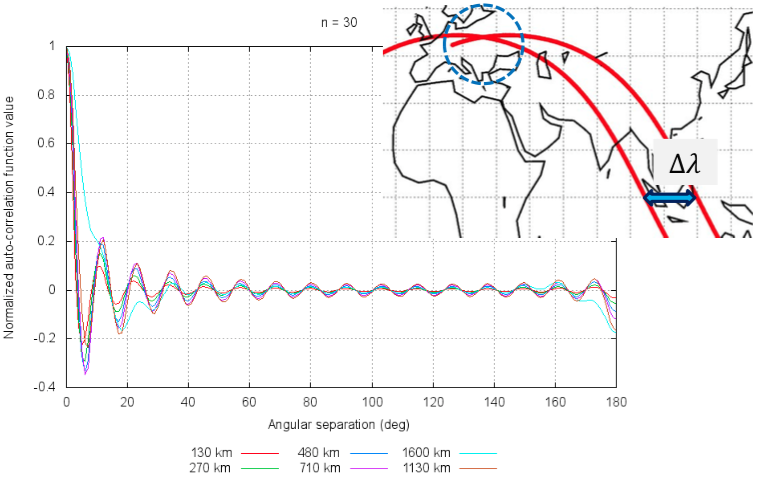
\includegraphics[width=\textwidth]{auto-correlation.png}
  \caption{Normalized auto-correlation function for the EIGEN-GL04C geopotential as a function of angular separation and the orbit altitude being the parameter. \label{fig:auto-correlation}} 
\end{figure}
\todo[Replace figure]{Replace \fig{fig:auto-correlation} using Tikz}

\subsection{Exemplary results}

\begin{figure}[h!]
  \centering
  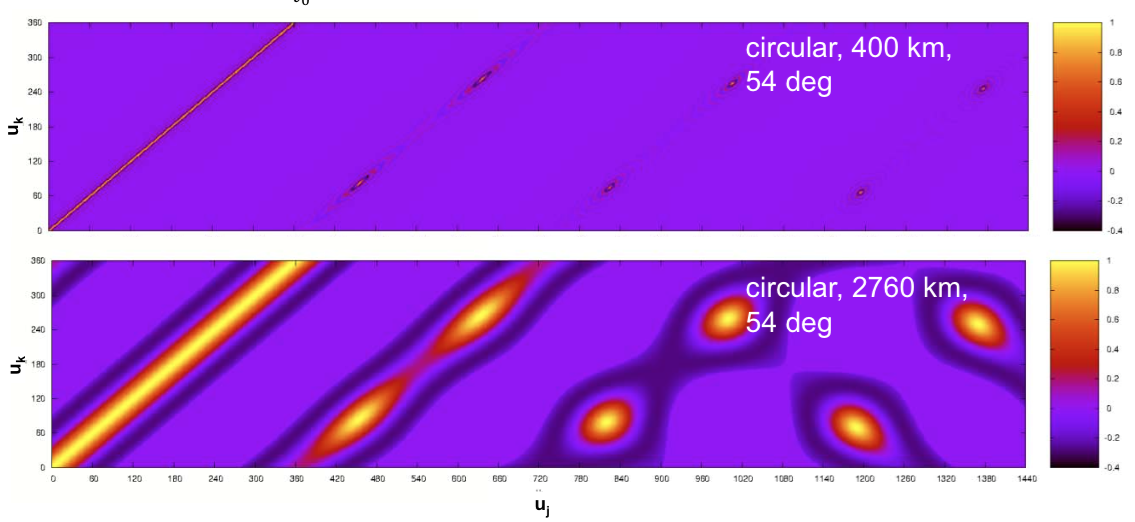
\includegraphics[width=\textwidth]{correlation-leo.png}
  \caption{Normalized auto-correlation function for two \gls{acr:leo} orbits, showing also the correlation of the current with subsequent orbits.\label{fig:correlation-leo}}
\end{figure}
\todo[Replace figure]{Replace \fig{fig:correlation-leo} using Tikz}

\begin{figure}[h!]
  \centering
  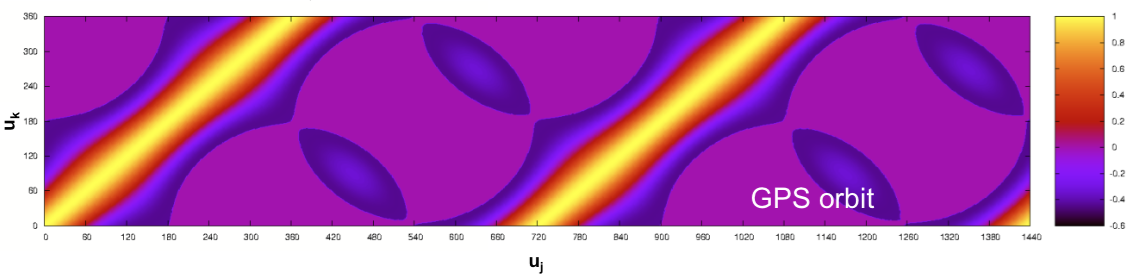
\includegraphics[width=\textwidth]{correlation-gps.png}
  \caption{Normalized auto-correlation function for \gls{acr:gps} orbits, showing also the correlation of the current with subsequent orbits. A typical picture for \SI{12}{\hour} resonance orbits.\label{fig:correlation-gps}}
\end{figure}
\todo[Replace figure]{Replace \fig{fig:correlation-gps} using Tikz}

\begin{figure}[h!]
  \centering
  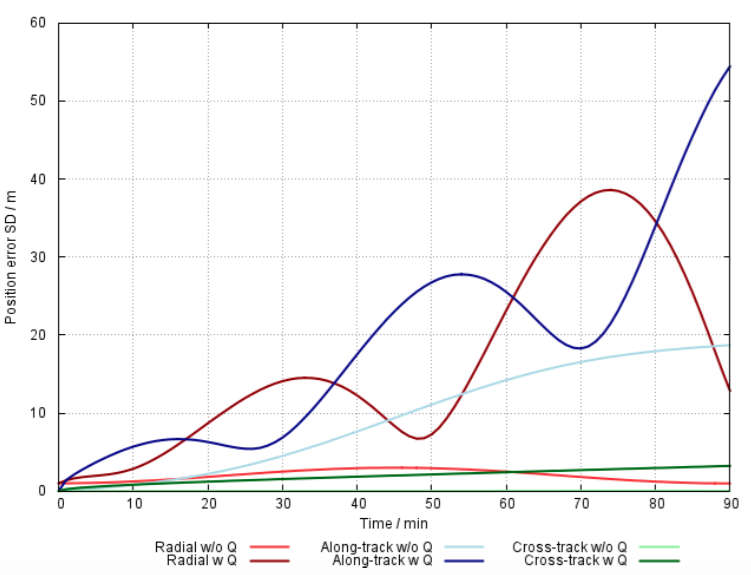
\includegraphics[width=\textwidth]{noise-results-matQ.png}
  \caption{Force model error contributions using a 30 $\times$ 30 geopotential, for an orbit at \SI{300}{\kilo\metre} and an inclination of \ang{50;;}.  \label{fig:noise-contributions}}
\end{figure}
\todo[Replace figure]{Replace \fig{fig:noise-contributions} using Tikz}




%------------------------------------------------------------------------------
%\bibliographystyle{plain}
%\bibliography{wp2report}
%------------------------------------------------------------------------------
%  \clearpage
 % \todo{Correct matrix in Eq. 4.144: d/drbf=... error in element 3,2} 
  % interpolation
 % \include{interpolation}
%  \clearpage

  % Autoconfiguration
 % \include{autoconfig}
%  \clearpage
  
  % verification and validation
  %------------------------------------------------------------------------------
\chapter{Verification \& Validation}
\label{cha:validation}
%------------------------------------------------------------------------------

%------------------------------------------------------------------------------
\section{Overview}
%------------------------------------------------------------------------------

In order to show that the implementation of \neptune{} was successful, performing a verification and validation process is essential. In this context, 
verification will always be referred to comparing a method to another comparable one. In contrast, validation means that the results are compared to a \textit{truth}.

A validation process was set up for the state vector propagation, using freely available \gls{acr:poe} data for distinct satellites. The selected satellites 
are:
\begin{itemize}
 \item Jason-1: Oceanography satellite. 
 \item \acrshort{acr:gps}: 32 satellites of the \gls{acr:gps} constellation
 \item \acrshort{acr:ers}-1 and \acrshort{acr:ers}-2: Earth observation satellites
 \item \acrshort{acr:icesat}: Earth observation satellite
\end{itemize}

The validation process was performed in two steps. The first step consists of using a \gls{acr:poe} of the satellite under consideration as the initial state 
vector for the numerical propagation in \neptune{}. The second step consists of taking multiple \gls{acr:poe}s and assume them to be observations in order to 
perform a differential correction to find an initial state vector, which is expected to provide more accurate results. The following settings were used for 
\neptune{}:
\begin{itemize}
 \item Cannon-ball model for each satellite
 \item \acrshort{acr:egm}96, \num{70}$\times$\num{70} geopotential
 \item \gls{acr:eop}
 \item \acrshort{acr:nrl}\acrshort{acr:msis}E-00 atmosphere model
 \item Lunisolar gravitational perturbations
 \item Solar radiation pressure
 \item Solid Earth and ocean tides
 \item Earth radiation pressure
\end{itemize}

Alternatively, the state vector propagation can also be verified against another validated numerical integration tool. The main advantage here would be that all relevant orbit regions can be analysed, while using \glspl{acr:poe} is only possible for distinct orbits.

For the propagation of the covariance matrix propagation and the noise matrix evaluation a \gls{acr:mc} approach was used for the verification of the routines 
as a validation was not possible due to a lack of available data.

\section{State vector propagation validation}

%\begin{itemize}
% \item Post-processing often achieves accuracies of 2-10 cm radial position \cite{vallado2007}
% \item \gls{acr:tle} achieves km-level accuracy, can be at about 400 m, or even 50-100 m in post processing using numerical methods \cite{vallado2007}
% \item First possibility: Take single state vector from a \gls{acr:poe} and propagate without modification, as \gls{acr:poe} is assumed to be within an 
%accuracy of 2-10 cm (radial position).
% \item Second possibility: Slightly perturb satellite state (1 m) and compare against \gls{acr:poe}
% \item Propagation span shall be about 7-14 days, which is a typical span for operational decisions.
% \item In the drag regime:
% \item Optical properties, e.g. for TOPEX, LAGEOS, etc. can be obtained via \cite{knocke1989}.
% \item Credit to University of Texas \gls{acr:csr}
% \end{itemize}

% \subsection{Laser Geodynamics Satellites (LAGEOS)}
% \gls{acr:lageos}
%  \begin{itemize}
%   \item Promising candidate for small perturbing forces (SRP, ERP, Tides) due to simple geometry and low level of drag
%   \item Satellite properties in \cite{knocke1989}, p.43
%  \end{itemize}

\subsection{Jason-1}

The oceanography mission Jason-1 was launched in December 2001 as a successor to the TOPEX/Poseidon mission. With an initial mass of \SI{500}{\kilogram} it reached its 
first orbit about \SIrange{10}{15}{\kilo\metre} below the target orbit of TOPEX/Poseidon at \SI{1337}{\kilo\metre} \cite{nasaJason2014}. It then moved to the same orbit with an along-track 
separation to TOPEX/Poseidon of about \SI{500}{\kilo\metre}. It is thus reasonable to assume that the mass of Jason-1 was lower than \SI{500}{\kilogram} after it reached its final orbit. 
In \cite{vallado2007} the mass was set to \SI{475}{\kilogram}. The other required satellite parameters, which were used in the propagation with \neptune{}, are shown in 
\tab{tab:val-jason-data}.
\begin{table}[h!]
 \centering
 \caption{Satellite parameters used for Jason-1.\label{tab:val-jason-data}}
 \begin{tabular}{lS}
  \toprule
  \textbf{Parameter} & \textbf{Value} \\
  \cmidrule{1-2}
  Mass / \si{\kilogram}                         & 475.0 \\
  Cross-section / \si{\metre\squared}  & 10.0 \\
  Drag coefficient          & 2.2 \\
  \acrshort{acr:srp} coefficient & 1.2 \\
  \bottomrule
 \end{tabular}
\end{table}
While the satellite mass, drag coefficient and \gls{acr:srp} coefficient were equal to the values used in \cite{vallado2007}, for the cross-section a value of 
\SI{10.0}{\metre\squared} was estimated, based on the fact that the area of the solar panels is about \SI{9.5}{\metre\squared} and the box-shaped satellite has dimensions of 
\SI{954}{\milli\metre}$\times$\SI{954}{\milli\metre}$\times$\SI{2218}{\milli\metre}\footnote{\url{http://www.eoportal.org/directory/pres_Jason1AltimetryMission.html}, accessed on 2014-03-03.}.
 
The \gls{acr:poe} data was obtained from the \acrshort{acr:legos}-\acrshort{acr:cls} via the \gls{acr:ids} 
website\footnote{\url{http://ids-doris.org/welcome.html}, accessed on 2014-03-03.} in the \gls{acr:sp3} format for a period between March 20, 2002 and April 21, 
2002. That period was also used as the propagation span within \neptune{}.

The results for a 24-day propagation starting on March 24, 2002, are shown in \fig{fig:val-jas-01} \todo[TikZ conversion]{Provide Tikz image instead of GNUplot png}.
\begin{figure}[!h]
 \centering
 %%plot 'valjas_1_000.rad' u ($1-52357.0):10 w l lw 2 lt rgb 'green' title 'Cross-track', \
%     'valjas_1_000.rad' u ($1-52357.0):9  w l lw 2 lt rgb 'red'   title 'Along-track', \
%     'valjas_1_000.rad' u ($1-52357.0):8  w l lw 2 lt rgb 'blue'  title 'Radial'

\begin{tikzpicture}[scale=1]

  \begin{axis}[
      height=0.6\textwidth,
      width=0.8\textwidth,
      xlabel = {Day since March 4, 2002},
      ylabel = {Error/km},
      y tick label style={
       /pgf/number format/.cd,
           fixed,
           fixed zerofill,
           precision=1,
       /tikz/.cd
      },
      xmin   = 0,
      xmax   = 24,
      %clip=false,
      %restrict x to domain=23:25,
      %x coord trafo/.code={\pgfmathparse{#1-5.0}\pgfmathresult} % x-offset MJD
      ymin   = -0.2,
      ymax   = 1.8,
      %xtick  = {250,300,...,600},
      ytick  = {-0.2,0,0.2,...,1.8},
      %minor x tick num={1},
      %minor y tick num={3},
      scaled ticks = true,
      ymajorgrids,
      %yminorgrids,
      xmajorgrids,
      %xminorgrids,
      legend entries={Along-track, Cross-track, Radial} ,
      legend style={at={(0.02,0.98)}, anchor=north west},
      legend cell align = left
  ]
    \addplot[red, thick, smooth]          table {06-Validation/data/valjas_1_along2.out};
    \addplot[green, thick, smooth]        table {06-Validation/data/valjas_1_cross2.out};
    \addplot[blue, thick, smooth]         table {06-Validation/data/valjas_1_radial2.out};
    
  \end{axis}
  
\end{tikzpicture}
 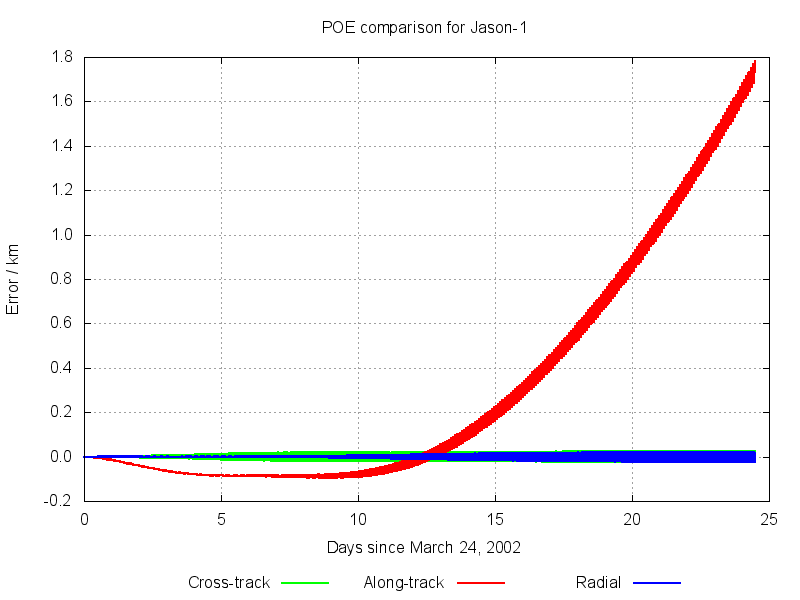
\includegraphics[width=0.85\textwidth]{val_jas_01.png}
 \caption{Comparison results for Jason-1.\label{fig:val-jas-01}}
\end{figure}
It can be seen that the error in the along-track component amounts to about one kilometre after three weeks of propagation.

A closer look at a smaller time interval of one day is shown in \fig{fig:val-jas-02} \todo[TikZ conversion]{Provide Tikz image instead of GNUplot png}.
\begin{figure}[!h]
 \centering
 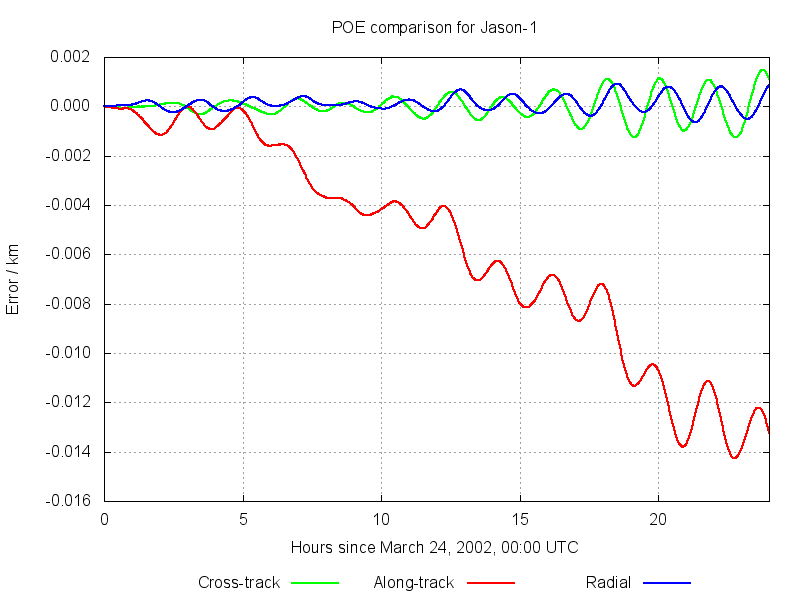
\includegraphics[width=0.85\textwidth]{val_jas_02.png}
 \caption{Comparing results for Jason-1 for a one-day propagation.\label{fig:val-jas-02}}
\end{figure}
The error in the along-track component is at about \num{14} metres after one day. The quite irregular looking evolution of the along-track error is basically due to 
the Solar and Earth radiation pressure contributions, as Jason-1 was modelled as a spherically shaped object. This becomes more obvious, when looking at the 
error evolution after switching these two perturbations off subsequently. In \fig{fig:val-jas-03} \todo[TikZ conversion]{Provide Tikz image instead of GNUplot png} the Earth radiation pressure (short-wave albedo and long-wave 
infrared) was switched off.
\begin{figure}[!h]
 \centering
 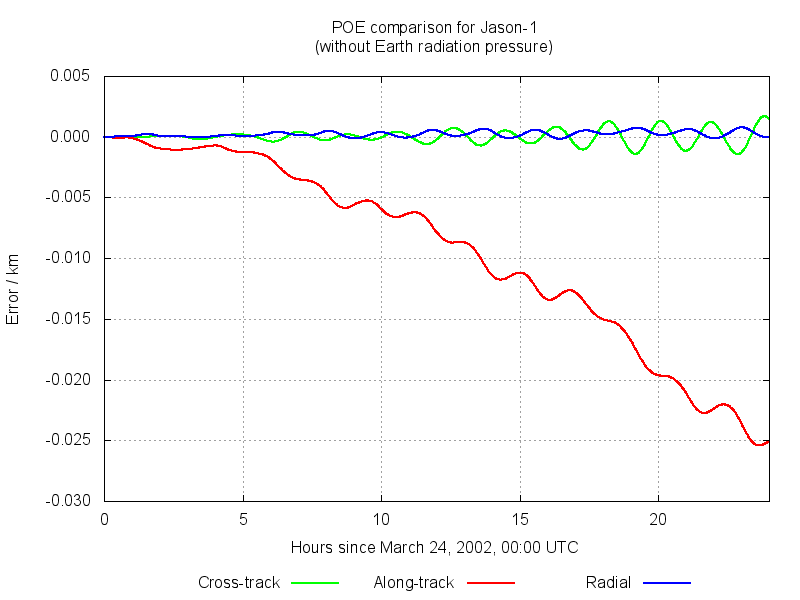
\includegraphics[width=0.85\textwidth]{val_jas_03.png}
 \caption{Comparing results for Jason-1 for a one-day propagation without Earth radiation pressure.\label{fig:val-jas-03}}
\end{figure}
The error increases to about 25 metres after one day, when Earth's radiation pressure is not considered. When solar radiation pressure is also switched off, 
the along-track error increases to about 65 metres after one day as shown in \fig{fig:val-jas-04}.
\begin{figure}[!h]
 \centering
 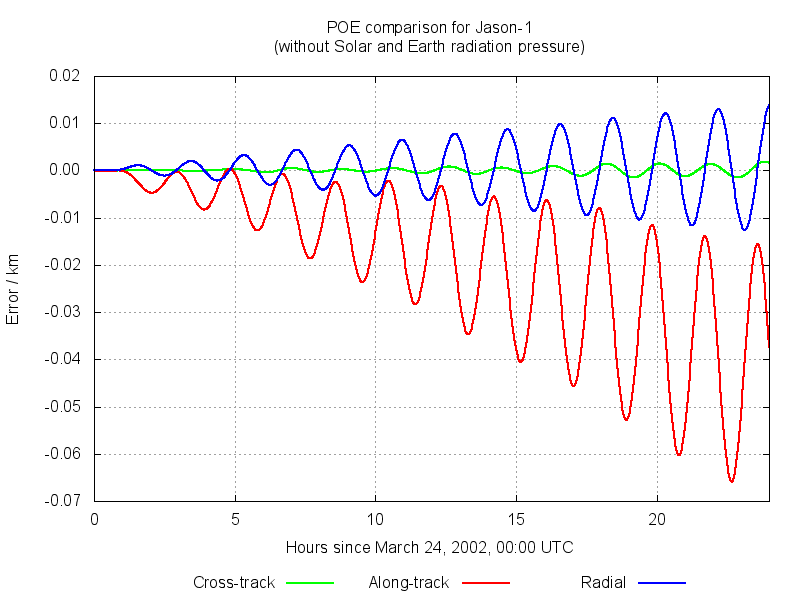
\includegraphics[width=0.85\textwidth]{val_jas_04.png}
 \caption{Comparing results for Jason-1 for a one-day propagation without Solar and Earth radiation pressure.\label{fig:val-jas-04}}
\end{figure}

\subsection{Global Positioning System (GPS)}

The validation using \gls{acr:gps} precision ephemerides is based on data available from the \gls{acr:nga} website \cite{nga2013}. The data was downloaded from 
the \gls{acr:nga} \acrshort{acr:ftp} server\footnote{\url{ftp://ftp.nga.mil/pub2/gps/pedata/}} for the year 2013. 

For the validation it is essential to use a time span free of any orbital maneuvers for the satellites under consideration. Therefore the so-called 
\gls{acr:nanu} messages were used, which are provided by the U.S. Coast Guard Navigation Center\footnote{\url{http://navcen.uscg.gov/?pageName=gpsAlmanacs}} 
for the \gls{acr:gps} satellites, containing information on which satellite is expected to have forecast outages for which period of time. A good 
overview on the available \gls{acr:nanu} messages for an individual year can also be found at the Celestrak website \cite{celestrak-nanu-2014}.

Extracting all the required information from the \gls{acr:nanu}s for 2013, one gets a good picture of which time frames are adequate to perform a validation 
for the complete \gls{acr:gps} constellation. The result of such an analysis is shown in \fig{fig:val-gps-nanu-2013}.
\begin{figure}[h!]
 \centering
 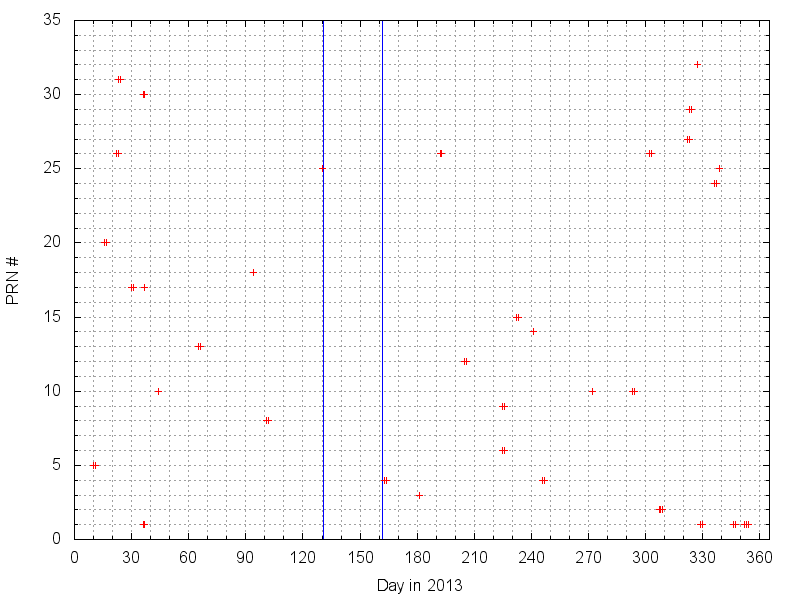
\includegraphics[width=0.85\textwidth]{nanu_summary_2013.png}
 \caption{Unusable ephemerides for all GPS satellites in 2013. The time span between the two vertical lines (blue) can 
be used in the validation analysis.\label{fig:val-gps-nanu-2013}}
\end{figure}
It can be seen that there is a window of approximately three weeks between day 131 and day 162 as indicated by the vertical blue lines, corresponding to a time frame of one month between May 11, 2013 and June 11, 2013.

The currently operational \gls{acr:gps} constellation consists of 32 satellites (as of February 2014) from the \textit{Block II} 
generation only \cite{gps2014} with satellites of the 
\textit{Block III} generation being under production. For the operational satellites a further subdivision is possible \cite{navcen2014}:
\begin{itemize}
 \item \textbf{Block IIA:} 8 operational, second generation, ``Advanced''
 \item \textbf{Block IIR:} 12 operational, ``Replenishment''
 \item \textbf{Block IIR(M):} 8 operational, ``Modernized''
 \item \textbf{Block IIF:} 4 operational, ``Follow-on''
\end{itemize}

It is important to consider the different types of Block II satellites in order to have an appropriate estimate of the cross-sectional area and the mass. In \tab{tab:val-gps-sats} the currently operational satellites are shown together with their \gls{acr:prn} code, the dimensions\footnote{Width across solar panels} 
and the mass, which were also used 
for the validation.
\begin{table}[h!]
 \centering
 \caption{Current GPS constellation as of February 26, 2014 \citep{navcen2014, about.com2014}.\label{tab:val-gps-sats}}
 \begin{tabular}{lp{5cm}lS}
 \toprule
  \textbf{Type} & \textbf{PRNs} & \textbf{Dim. W$\times$D$\times$H / \si{\milli\metre}} & \textbf{Mass / \si{\kilogram}} \\
  \cmidrule{1-4}
  Block IIA    & 3,  4,  6,  8,  9, 10, 26, 32      &        5300 $\times$ 3400 $\times$ 3400 & 840 \\
  Block IIR    & 2, 11, 13, 14, 16, 18-23, 28       & 11\ 400 $\times$ 1956 $\times$ 2210 & 1127 \\
  Block IIR(M) & 5,  7, 12, 15, 17, 29, 30$^*$, 31  & 11\ 400 $\times$ 1956 $\times$ 2210 & 1127 \\
  Block IIF    & 1, 24, 25, 27$^{**}$               & 11\ 820 $\times$ 2032 $\times$ 2235 & 1465 \\
  \bottomrule
  \multicolumn{1}{r}{\footnotesize $^*$}    & \multicolumn{3}{l}{\footnotesize PRN30 was launched on Feb 21, 2014 \citepalias{nanu2014018} and is not considered in 
the validation.} \\
  \multicolumn{1}{r}{\footnotesize $^{**}$} & \multicolumn{3}{p{12cm}}{\footnotesize PRN27 was launched on May 15, 2013 \citepalias{nanu2013031} and is not considered 
in the validation.} \\   
 \end{tabular}
\end{table}
From the 32 active satellites in the constellation, for the selected validation time frame only 30 satellites may be used. \acrshort{acr:prn}27 was launched 
within that time span on May 15, 2013 \citepalias{nanu2013031} and was fully operational from June 21, 2013 \citepalias{nanu2013035}, so that it could not be used in the validation. Also, \acrshort{acr:prn}30 was launched on February 21, 2014 \citepalias{nanu2014018} and is currently in its testing phase.

For the simulations by \neptune{} it is required to estimate the cross-section of the GPS satellites based on the dimensions as specified in different sources for the different types of Block II objects. As for satellites in the GPS constellation the effective cross-section relative to the Sun's direction is significant, it was assumed that the full area of the solar panels contributes to the total cross-section. For the main body, the average of the three different surfaces of the rectangular cuboid (box) was computed. The total cross-section as well as the drag and \gls{acr:srp} parameter, which were used in the validation, are shown in \tab{tab:val-gps-sim-data}.
\begin{table}[h!]
 \centering
 \caption{Cross-section, \gls{sym:c_d} and \gls{sym:c_srp} of \acrshort{acr:gps} satellites used in the validation.\label{tab:val-gps-sim-data}}
 \begin{tabular}{lSSS}
  \toprule
  	\textbf{Type} & \textbf{Cross-section / \si{\metre\squared}} & \textbf{\gls{sym:c_d}} & \textbf{\gls{sym:c_srp}} \\
  \cmidrule{1-4}
  Block IIA       &     18.02 & 2.2 & 1.3\\
  Block IIR      &     22.63 & 2.2 & 1.3\\
  Block IIR(M) &     22.63 & 2.2 & 1.3\\
  Block IIF       &     24.29 & 2.2 & 1.3\\
  \bottomrule
 \end{tabular}
\end{table}

The \gls{acr:poe} data for \gls{acr:gps} satellites is obtained in the SP3 format \citep{remondi1989}, where the cartesian state vectors in five minute intervals are given in the \acrshort{acr:wgs}84 frame. In \neptune{} the \gls{acr:itrf} is used, however, \acrshort{acr:wgs}84 is closely aligned to the 
\gls{acr:itrf} \citep{tapley2004} so that no coordinate transformation was required at this point. Instead, the ephemerides were converted to \gls{acr:gcrf} in order to be compared with the trajectory as propagated by \neptune{}. Some exemplary results are shown in the following.
\begin{figure}[!h]
 \centering
 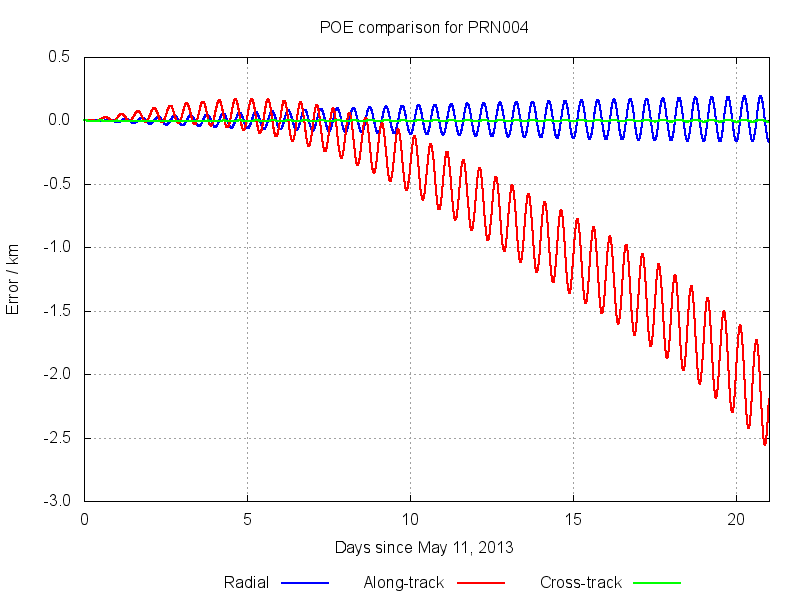
\includegraphics[width=0.85\textwidth]{val_gps_prn04.png}
 \caption{Comparison results for PRN04.\label{fig:val-gps-prn04}}
\end{figure}

\begin{figure}[!h]
 \centering
 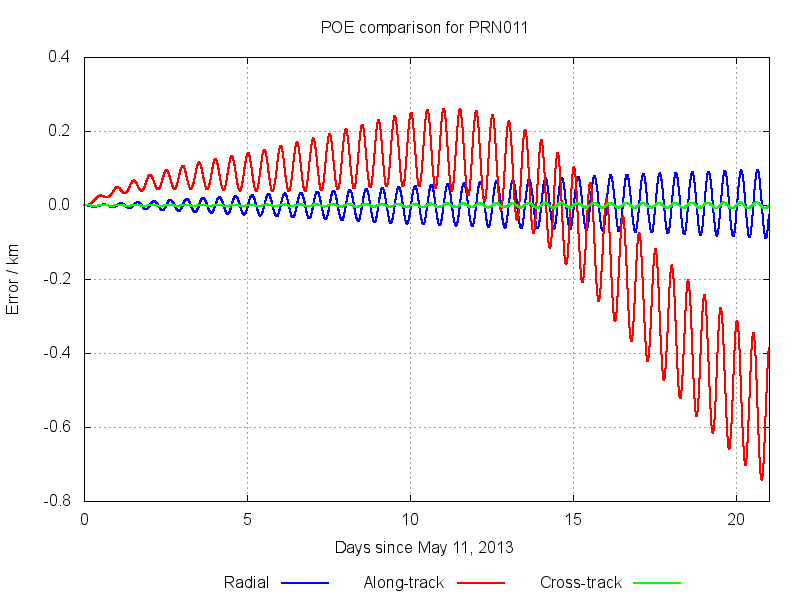
\includegraphics[width=0.85\textwidth]{val_gps_prn11.png}
 \caption{Comparison results for PRN11.\label{fig:val-gps-prn11}}
\end{figure}

In \fig{fig:val-gps-prn04} the result for \acrshort{acr:prn}04 is shown. The error in the along-track component is about \SI{2.5}{\kilo\metre} after 21 days. However, there were also examples, where the error was significantly lower, as for example in the case of \acrshort{acr:prn}11, where the along-track error is at about \SI{700}{\metre} after the same period of 21 days. It can also be seen that the radial error for \acrshort{acr:prn}11 is lower than for \acrshort{acr:prn}04, which, of 
course, correlates with the evolution of the along-track component.

A third example is shown in \fig{fig:val-gps-prn09} for \acrshort{acr:prn}09. Here, the along-track error increases to about \SI{3.5}{\kilo\metre} after 21 days, while the radial error is almost at \SI{500}{\metre}. 

\begin{figure}[!h]
 \centering
 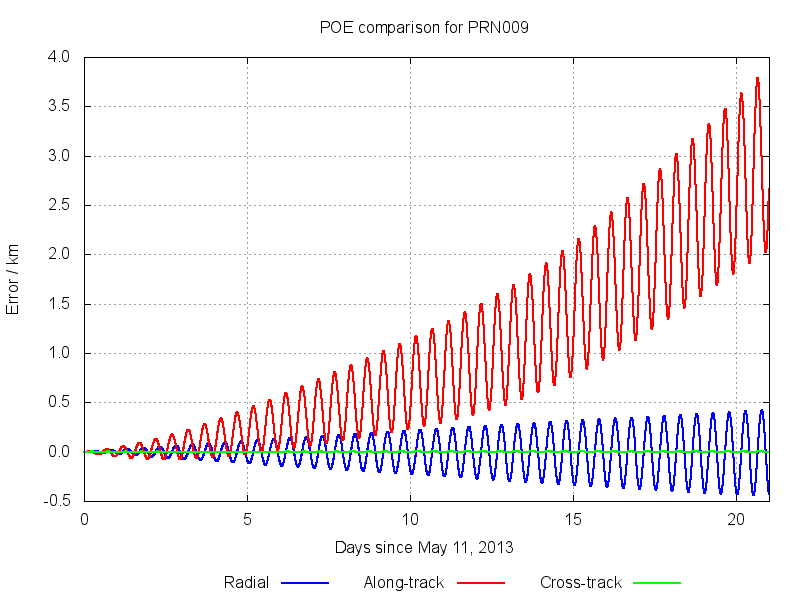
\includegraphics[width=0.85\textwidth]{val_gps_prn09.png}
 \caption{Comparison results for PRN09.\label{fig:val-gps-prn09}}
\end{figure}

The errors in all examples are showing a fluctuation with a period of one orbit, which is typical for a model misalignment. This was expected, as the first \gls{acr:poe} was selected to be the initial state for \neptune{} which then propagates with another model as compared to the one used for the \gls{acr:poe} generation.

\subsection{European Remote Sensing Satellites (ERS-1 and -2)}

The first mission \acrshort{acr:ers}-1 was launched on July 17, 1991 and was accompanied by \acrshort{acr:ers}-2 on April 21, 1995 with both objects put into a sun-synchronous orbit between \SIrange{782}{785}{\kilo\metre}
\footnote{\url{https://earth.esa.int/web/guest/missions/esa-operational-eo-missions/ers/satellite}\label{foot:esa}}. From \acrshort{acr:esa}'s 
website$^{\ref{foot:esa}}$ an initial estimate for the satellite parameters was derived, shown in \tab{tab:val-ers-data}. Missing parameters, being the drag and \gls{acr:srp} coefficients, were taken from \cite{vallado2007}.
\begin{table}[h!]
 \centering
 \caption{Satellite parameters used for \gls{acr:ers}-1 and \gls{acr:ers}-2.\label{tab:val-ers-data}}
 \begin{tabular}{lS}
 \toprule
  	\textbf{Parameter} & \textbf{Value} \\
  \cmidrule{1-2}
  Mass / \si{\kilogram}                 & 2300 \\
  Cross-section / \si{\metre\squared}     & 35.0 \\
  Drag coefficient          & 2.5 \\
  \acrshort{acr:srp} coefficient & 1.0 \\
  \bottomrule
 \end{tabular}
\end{table}

For \acrshort{acr:ers}-1 the first propagation was performed starting on August 4, 1991. The result is shown in \fig{fig:val-ers1-01}.
\begin{figure}[!h]
 \centering
 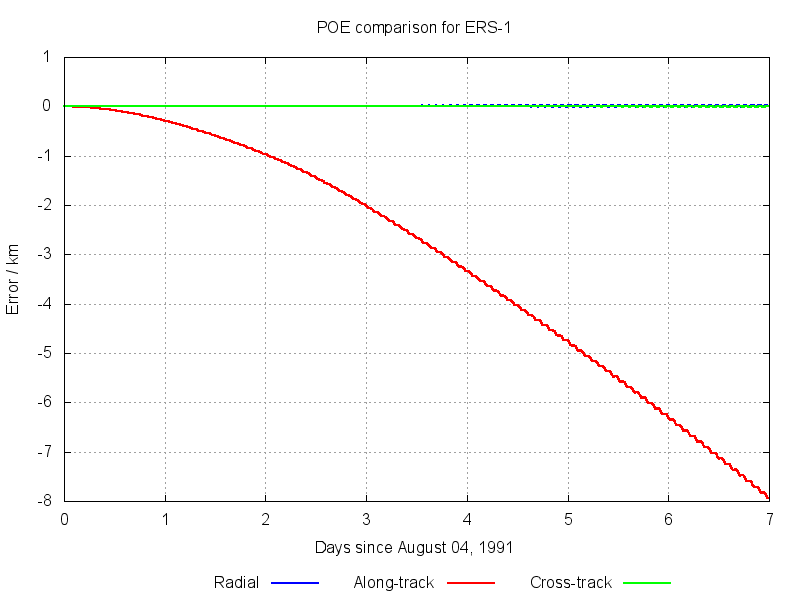
\includegraphics[width=0.85\textwidth]{valers1_1.png}
 \caption{Comparison results for ERS-1 for a one-week propagation.\label{fig:val-ers1-01}}
\end{figure}
After a one-week propagation, the accumulated error in the along-track component is about eight kilometers. 

For a shorter time frame of about six hours starting from the initial epoch, the error is shown in \fig{fig:val-ers1-02}.
\begin{figure}[!h]
 \centering
 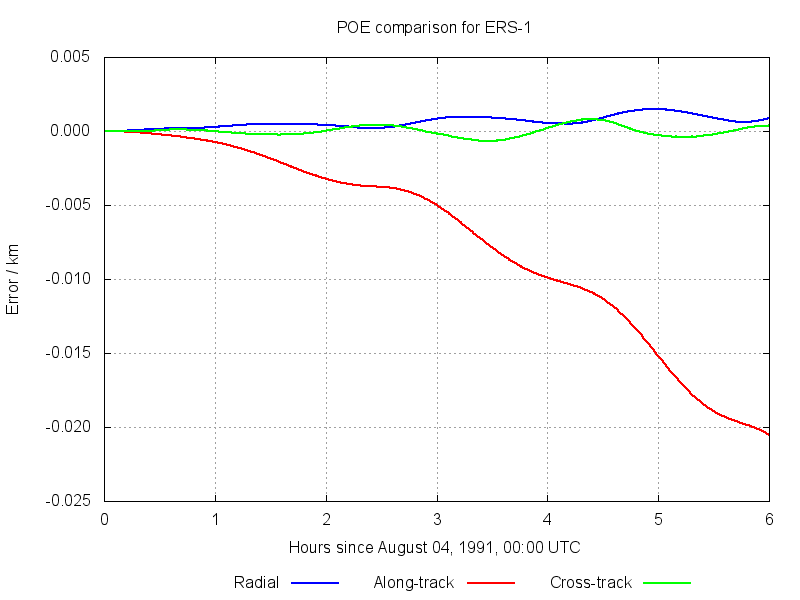
\includegraphics[width=0.85\textwidth]{valers1_2.png}
 \caption{Comparison results for ERS-1 for a six-hour propagation.\label{fig:val-ers1-02}}
\end{figure}
The radial error increases after each revolution by about one meter which leads to the build-up in along-track error. This indicates, as the radial error is positive, that \acrshort{acr:ers}-1 was decaying faster than the propagated orbit of \neptune{}, as in general the error was computed via:
\begin{equation}
  \Delta \vec{r} = \vec{r}_{NEPTUNE} - \vec{r}_{ERS}
\end{equation}
While the considered epoch for \acrshort{acr:ers}-1 was within a period of increased solar activity, for \acrshort{acr:ers}-2 it was looked at whether the situation changes during low solar activity. Therefore, the initial epoch was selected to be at September 8, 1995. Also, the cross-section was adapted to \SI{11}{\metre\squared} and the mass set to \SI{2200}{\kilogram} to make the results comparable to the ones obtained in \cite{vallado2007}. The errors for a propagation span of one week are shown 
in \fig{fig:val-ers2-01}.
\begin{figure}[!h]
 \centering
 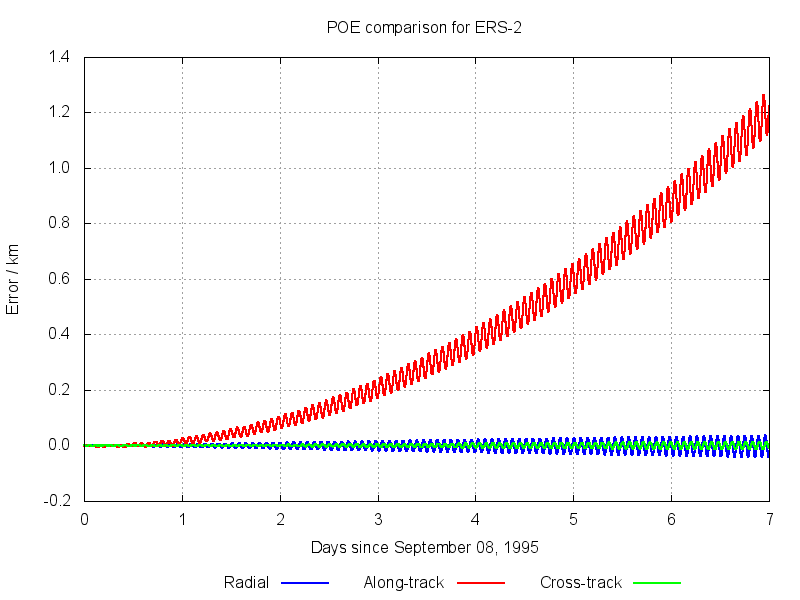
\includegraphics[width=0.85\textwidth]{valers2_1.png}
 \caption{Comparison results for ERS-2 for a one-week propagation.\label{fig:val-ers2-01}}
\end{figure}
It can be seen that the resulting error after seven days in the along-track component is about \SI{1.2}{\kilo\metre}. It was at about \SI{10}{\kilo\metre} when using the satellite parameters as given in \tab{tab:val-ers-data} which were used for \acrshort{acr:ers}-1. However, using another set of parameters for \acrshort{acr:ers}-1, for example as used for \acrshort{acr:ers}-2 in \fig{fig:val-ers2-01}, did not provide better results. It can thus be argued that solar activity has a significant influence on the prediction accuracy, even if the solar and geomagnetic activity data used in the simulation was observed data for the considered 
propagation spans. 

\subsection{Ice, Cloud, and land Elevation Satellite (ICESat)}

\gls{acr:icesat} was part of \acrshort{acr:nasa}'s Earth observation system between 2003 and 2009 and its mission was to measure the ice sheet mass balance, cloud 
and aerosol heights, as well as perform land topography and analyse vegetation characteristics \footnote{\url{http://icesat.gsfc.nasa.gov/}}. The 
\gls{acr:poe}s for \gls{acr:icesat} were obtained from the \acrshort{acr:ftp} server of the \gls{acr:csr} at the University of Texas \citep{csr2014} for a time frame between September 24, 2003 and November 18, 2003.

As \gls{acr:icesat} was operated in an orbit at about \SI{600}{\kilo\metre} altitude, atmospheric drag was providing a significant contribution to the orbital evolution. 
Therefore, it is essential to have a good estimate of the ballistic parameter. In a similar study by \cite{vallado2007}, an initial mass of \SI{970}{\kilogram} was reduced to about \SI{950}{\kilogram}, assuming that some maneuvering fuel had been spent, to be used in the simulation for February 2003.

For the \neptune{} validation and the time frame between September and November 2013, a value of \SI{950}{\kilogram} was used as a starting value. Also, in 
\cite{vallado2007} further required values are given, which were used in the following analyses and are shown in \tab{tab:val-ice-data}.
\begin{table}[h!]
 \centering
 \caption{Satellite parameters used for \gls{acr:icesat}.\label{tab:val-ice-data}}
 \begin{tabular}{lS}
 \toprule
	\textbf{Parameter} & \textbf{Value} \\
  \cmidrule{1-2}
  Cross-section / \si{\metre\squared}   & 2.0 \\
  Drag coefficient          & 2.2 \\
  \acrshort{acr:srp} coefficient & 1.0 \\
  \bottomrule
 \end{tabular}
\end{table}

The first analysis was done for a propagation span of a few days, starting at September 25, 2003, 21:00 \acrshort{acr:utc}. The results can be seen in 
\fig{fig:val-ice-01}.
\begin{figure}[!h]
 \centering
 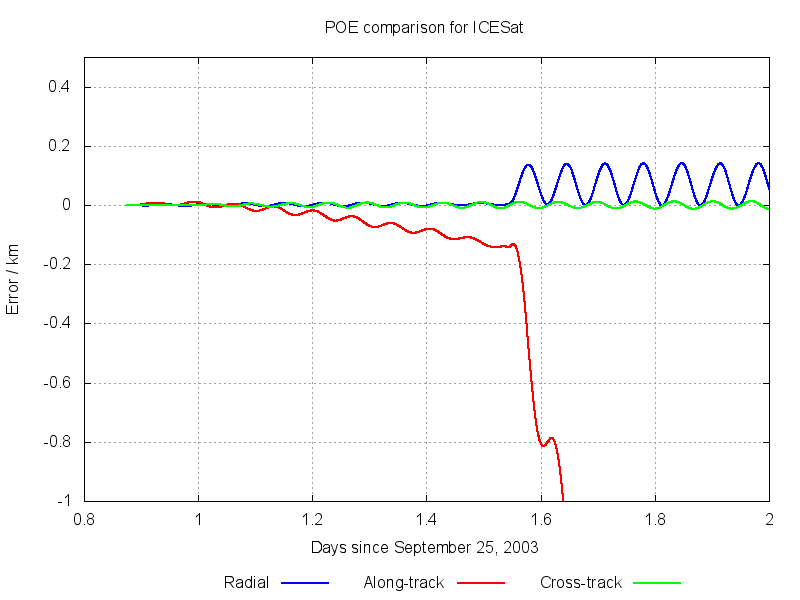
\includegraphics[width=0.85\textwidth]{valice01.png}
 \caption{Comparison results for ICESat showing a maneuver on September 26, 2003.\label{fig:val-ice-01}}
\end{figure}
While initially the errors in all three components are in the order of magnitude between \SIrange{10}{100}{\metre} with the along-track component showing an expected drift, on September 26, 2003 a maneuver can be identified, which manifests itself through a sudden change in slope for the along-track error and a sudden increase in the 
mean radial error. 
For the next analysis, the initial epoch was set to September 27, 2003, 21:00 \gls{acr:utc}, which is about one and a half days beyond the previous maneuver. 
As can be seen in \fig{fig:val-ice-02}, for a period free of maneuvers, the along-track error amounts to about one kilometer after about three days of 
propagation.
\begin{figure}[!h]
 \centering
 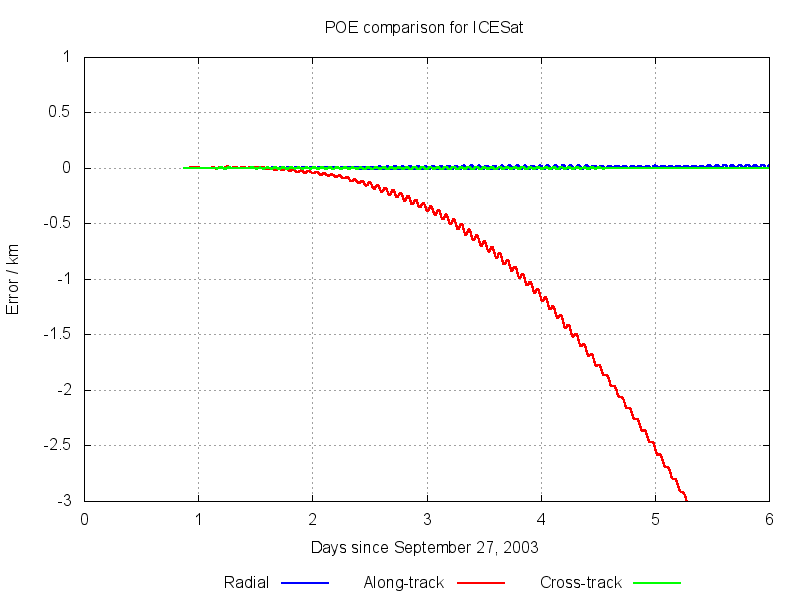
\includegraphics[width=0.85\textwidth]{valice02.png}
 \caption{Comparison results for ICESat for about four days after September 27, 2003, 21:00 UTC.\label{fig:val-ice-02}}
\end{figure}
This behaviour is expected in the presence of atmospheric drag, which becomes even more obvious when looking at the radial component alone as shown in 
\fig{fig:val-ice-03}.
\begin{figure}[!h]
 \centering
 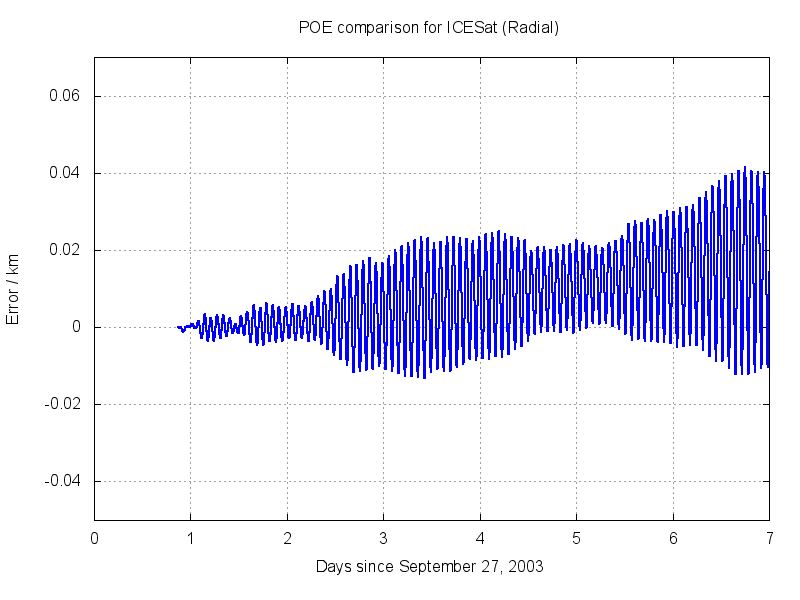
\includegraphics[width=0.85\textwidth]{valice03.png}
 \caption{Comparison results for ICESat: Radial error after September 27, 2003, 21:00 UTC.\label{fig:val-ice-03}}
\end{figure}
Here, the radial error shows a drift which means that \gls{acr:icesat} was descending with a faster rate than what \neptune{} predicted, as the error, in 
general, was computed by:
\begin{equation}
 \Delta \vec{r} = \vec{r}_{NEPTUNE} - \vec{r}_{ICESat}
\end{equation}
A faster descent would suggest that \gls{acr:icesat} had a lower mass (or a higher cross-section) as was initially assumed. Due to the maneuver on September 
26, it could be possible that the mass after that maneuver was below \SI{950}{\kilogram}. This seems to be even more reasonable when considering the fact that the mass 
estimate is based on \cite{vallado2007}, where the analysis was done for February 2003, with a few possible additional maneuvers until September 2003. Therefore, another validation run was performed after decreasing the mass to \SI{900}{\kilogram} and the result is shown in \fig{fig:val-ice-04}.
\begin{figure}[!h]
 \centering
 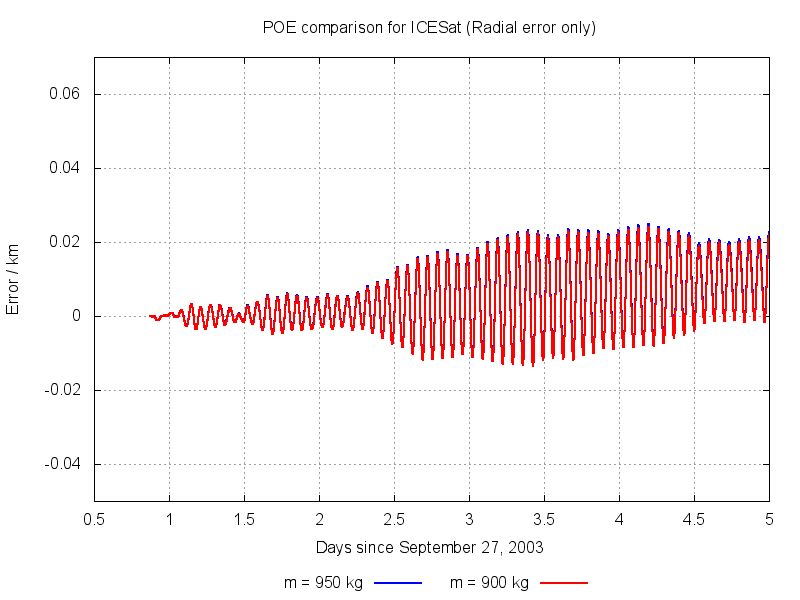
\includegraphics[width=0.85\textwidth]{valice04.png}
 \caption{Comparison results for ICESat: Radial error for a different initial mass.\label{fig:val-ice-04}}
\end{figure}
It can be seen that a reduced mass does not affect the result significantly. 

In \cite{vallado2007} it is mentioned that \gls{acr:icesat} may fly in a ``sailboat'' orientation, where the solar panels contribute most in velocity direction. A value of \SI{5.21}{\metre\squared} is given in \cite{vallado2007} together with an 
adapted drag coefficient of \gls{sym:c_d}=\num{2.52}. The result for this simulation is shown in \fig{fig:val-ice-05}.
\begin{figure}[!h]
 \centering
 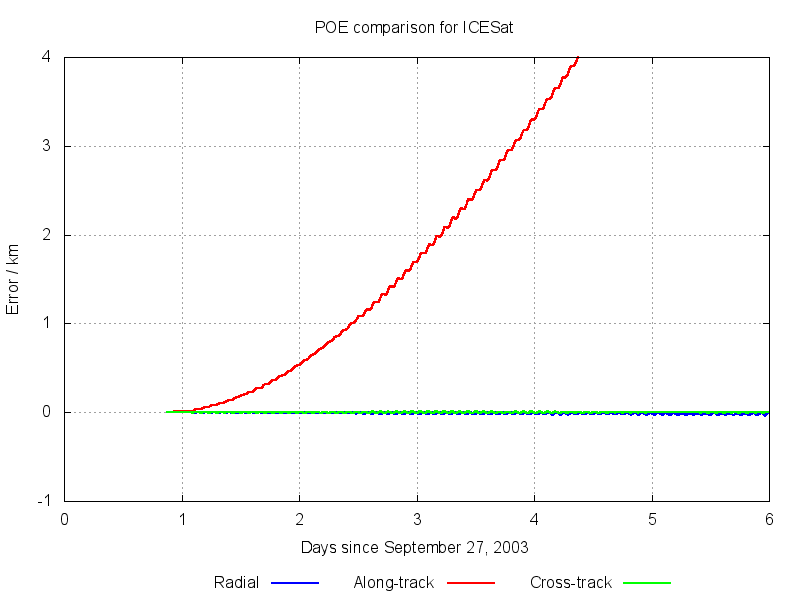
\includegraphics[width=0.85\textwidth]{valice05.png}
 \caption{Comparison results for ICESat: Error in ``sailboat'' orientation mode.\label{fig:val-ice-05}}
\end{figure}
It can be seen that the along-track error in this case is positive which means that the propagation by \neptune{} is trailed by \gls{acr:icesat} meaning that 
\neptune{} now results in predicting a too fast decay. As the error is at about one kilometer after two days - as compared to the same along-track error after 
three days in \fig{fig:val-ice-02} - a ``sailboat'' orientation seems unlikely for this period. However, an orientation somewhere in between the two analysed 
cases should provide a better solution, which is exemplarily shown in \fig{fig:val-ice-06} for a cross-section of \SI{3.0}{\metre\squared}.
\begin{figure}[!h]
 \centering
 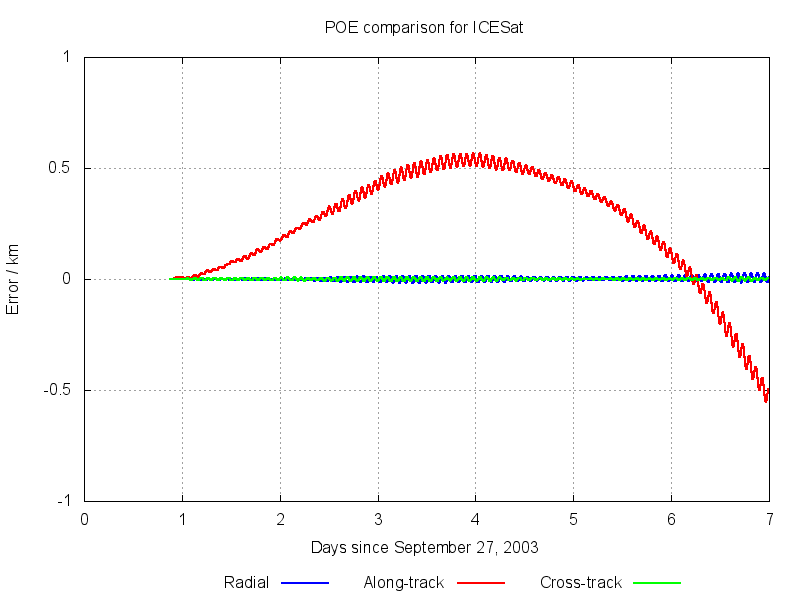
\includegraphics[width=0.85\textwidth]{valice06.png}
 \caption{Comparison results for ICESat: Error for a cross-section of \SI{3.0}{\metre\squared}.\label{fig:val-ice-06}}
\end{figure}

\section{Covariance matrix propagation verification}

The verification of the covariance matrix propagation in \neptune{} was done by a \gls{acr:mc} analysis. Therefore, a dedicated tool was developed: \cover{} (Covariance Verification). Its task, as shown in \fig{fig:val-cover-scheme}, is to receive the initial covariance matrix used by \neptune{} and to generate an object cloud representing the underlying statistics from the uncertainties in the state vector.
\begin{figure}[!h]
  \centering
  \setlength{\abovecaptionskip}{0.5cm}
     
  \begin{tikzpicture}[scale=0.7, transform shape, node distance=0.5cm, >=latex]
 
    \node (cover)     [redbox] 				{\textbf{COVER}};
    \node (input)     [bluebox, below =of cover]  	{Read input file: cover.inp};
    \node (inpfile)   [speicher, right=of input]  	{Input};
    \node (cloud)     [bluebox, below =of input]  	{Generate object cloud based on variance/covariance matrix};
    \node (loop_time) [branch, below=of cloud]		{\textbf{Loop:} Time};
    \node (time)      [bluebox, right=of loop_time]     {Increment time};
    \node (parent)    [bluebox, below=of time]          {Propagate parent's state and covariance};
    \node (loop_obj)  [branch, below=of parent]		{\textbf{Loop:} Objects};
    \node (objects)   [bluebox, below right=0.5cm and 1cm of loop_obj]      {Propagate object's state};
    \node (end1)      [branch, below=1cm of loop_obj]	{\textbf{End?}};
    
    \node (uvw)       [bluebox, below=of end1]       	{Convert states to UVW frame};
    \node (stats)     [bluebox, below=of uvw]        	{Process statistics};
    \node (output1)   [bluebox, below =of stats]     	{Write line to output: $<$RUNID$>$.cov};
    \node (output2)   [bluebox, below =of output1]   	{Write line to output: $<$RUNID$>$.prop.cov};
    \node (prop_file) [speicher, right=of output2]     	{Propagated covariance matrix};
    \node (cov_file)  [speicher, right=of output1]   	{Object cloud statistics};
    \node (end2)      [branch, below=13cm of loop_time]	{\textbf{End?}};
    \node (end)       [redbox, below=of end2]          	{\textbf{End}};


    \draw [->] (cover)     to (input);
    \draw [->] (inpfile)   to (input);
    \draw [->] (input)     to (cloud);
    \draw [->] (cloud)     to (loop_time);
    \draw [->] (loop_time) to (time);
    \draw [->] (time)      to (parent);
    \draw [->] (parent)    to (loop_obj);
    \draw [->] (loop_obj)  -| (objects);
    \draw [->] (end1)      to (loop_obj);
    \draw [->] (end1)      to (uvw);
    \draw [->] (uvw)       to (stats);
    \draw [->] (stats)     to (output1);
    \draw [->] (output1)   to (cov_file);
    \draw [->] (output1)   to (output2);
    \draw [->] (output2)   to (prop_file);
    \draw [->] (end2)      to (loop_time);
    \draw [->] (end2)      to (end);
% 
    \draw [->] (objects.south) |- (end1.east);
    \draw [->] (output2.south) |- (end2.east);

  \end{tikzpicture}
  \caption{Schematic overview of the \cover{} tool.}
  \label{fig:val-cover-scheme}
\end{figure}

As the radius and the velocity component errors present in the variance/covariance matrix are correlated, a Cholesky decomposition has to be performed. For the 
covariance matrix \gls{sym:P} the Cholesky decomposition is defined as:
\begin{equation}
 \gls{sym:P} = \gls{sym:L}\cdot\gls{sym:L}^T
\end{equation}
It is assumed that the initial errors in the state vector are normally distributed, so that random variables \gls{sym:Z} are computed according to a standard 
normal distribution:
\begin{equation}
 \gls{sym:Z} = \mathcal{N}\left(0,1\right)
\end{equation}
Then, for each object, the state vector can be sampled using six random numbers (for position and velocity), given via the vector $\gls{sym:z}_i = 
\left[\gls{sym:Z}_1,\ldots,\gls{sym:Z}_6\right]$ and the mean $\overline{\gls{sym:state}}$, which is the associated state vector:
\begin{equation}
 \gls{sym:state}_i = \gls{sym:L}\cdot\gls{sym:z}_i + \overline{\gls{sym:state}}
\end{equation}

For each generated object an individual \neptune{} propagation run for the sampled state vector to a certain reference epoch is performed. At this epoch the 
object cloud is processed to extract its statistics and form the covariance matrix for that point in time again. The result is then compared to the numerical 
integration of the covariance matrix as implemented in \neptune{}. 

The verification process of the covariance matrix propagation contained different scenarios with varying initial covariance matrix, as defined in the following 
list:
\begin{enumerate}
 \item Propagation of object cloud considering only the central body force.
 \item Scenario 1 + geopotential with order $\gls{sym:geo_n}=2$.
 \item Scenario 1 + geopotential with order $\gls{sym:geo_n}>2$.
 \item Scenario 1 + atmospheric drag
\end{enumerate}

\paragraph{Scenario 1: Central body force}

In the first scenario, only the central body force was used for the object cloud consisting of one parent object (identical to the state vector corresponding 
to the covariance matrix) and 499 generated objects according to the uncertainty in the state.

The first example for an initial radial error of \SI{1}{\metre}, and no error in the other components, is shown in \fig{fig:val-cov-scen1-01} for a circular orbit at \SI{300}{\kilo\metre} altitude and \ang{50;;} inclination.
\begin{figure}[h!]
  \centering
  \subfigure[Position]{\label{fig:val-cov-scen1-01a} 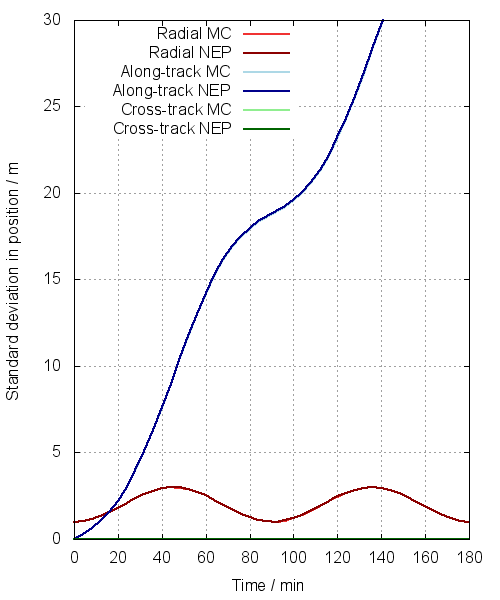
\includegraphics[width=0.4\textwidth]{2B_1_rad.png}}
  \hspace{1cm}
  \subfigure[Velocity]{\label{fig:val-cov-scen1-01b} 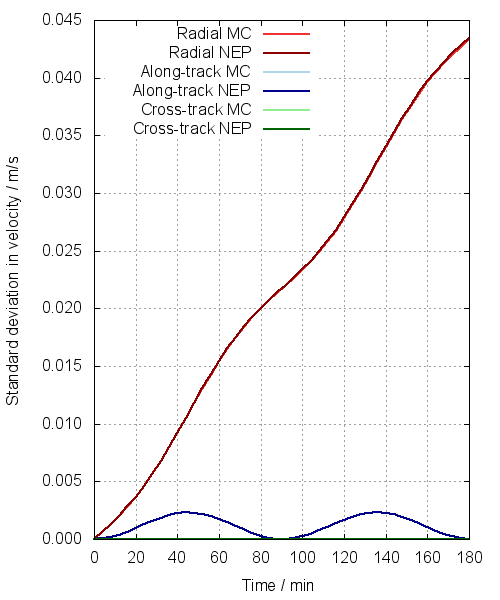
\includegraphics[width=0.4\textwidth]{2B_1_vel.png}}
  \caption{Comparing MC analysis results to \neptune{} covariance matrix propagation using a \SI{60}{\second} integration step size for an initial radial error of \SI{1}{\metre}.\label{fig:val-cov-scen1-01}}
\end{figure}
An error in radial position only leads to a drift in the along-track error as the orbital period is directly affected by the radial component. The latter shows an oscillation with the minimum being at \SI{1}{\metre} and the maximum reaching \SI{3}{\metre} after half an orbit. What can also be observed is that there is no error in the 
orbit normal component as should be expected for a two-body scenario.

It can be seen that there is almost no difference between the numerical propagation in \neptune{} as compared to the results from the \gls{acr:mc} analysis. In \fig{fig:val-cov-scen1-01a} and \fig{fig:val-cov-scen1-01b} the correlation between the along-track position error and the radial velocity error, as well as the correlation between the radial position and along-track velocity component, can be nicely seen. 

The next example in \fig{fig:val-cov-scen1-02} shows the standard deviation evolution for an initial error of \SI{1}{\metre\per\second} for the radial velocity only for the same orbit at \SI{300}{\kilo\metre} altitude and \ang{50;;} inclination. 
\begin{figure}[h!]
  \centering
  \subfigure[Position]{\label{fig:val-cov-scen1-02a} 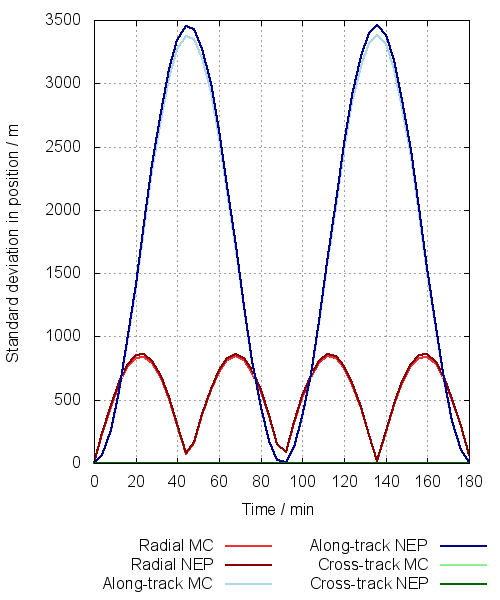
\includegraphics[width=0.4\textwidth]{2B_2_rad.png}}
  \hspace{1cm}
  \subfigure[Velocity]{\label{fig:val-cov-scen1-02b} 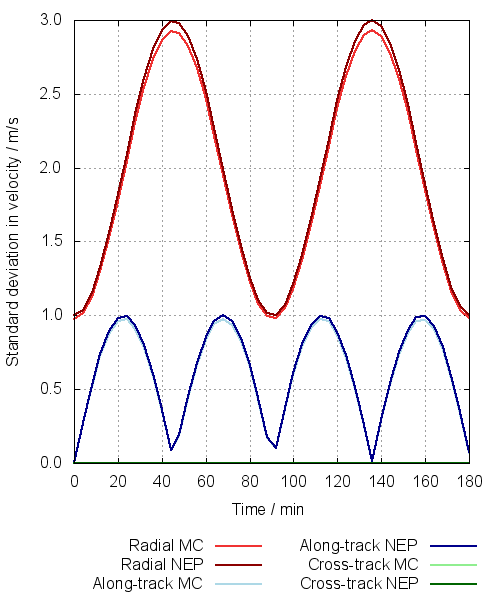
\includegraphics[width=0.4\textwidth]{2B_2_vel.png}}
  \caption{Comparing MC analysis results to \neptune{} covariance matrix propagation using a \SI{60}{\second} integration step size for an initial velocity error of \SI{1}{\metre\per\second}.\label{fig:val-cov-scen1-02}}
\end{figure}
Once again the results show a close alignment between the \gls{acr:mc} approach and \neptune{}'s integration. However, the along-track position error difference at about half an orbit is about \SI{80}{\kilo\metre}, while the error in the radial velocity at the same time is in the order of magnitude of \SI{0.1}{\metre\per\second}. 

This, however, is not indicating an erroneous implementation but is due to the fact that only 500 objects have been used. If the number is increased to 2000 objects, for example, the difference after half an orbit reduces to about \SI{63}{\kilo\metre} in along-track position error and about \SI{0.06}{\metre\per\second} in radial velocity error. 
Increasing the number even further to \num{10000} objects in the \gls{acr:mc} approach leads to a further decrease with the along-track position error difference 
being at about \SI{27}{\kilo\metre} and the radial velocity error difference at \SI{0.025}{\metre\per\second}. Thus, the results obtained by the \gls{acr:mc} analysis are converging towards the 
results from the numerical integration by \neptune{} for an increasing number of objects, which should be expected from the \textit{law of large numbers}.

\paragraph{Scenario 2: Geopotential with order $\gls{sym:geo_n}=2$}

In \sect{sec:propagation-covariance-set-integration-geopotential} the model for the integration of the state error transition matrix under consideration of the 
geopotential is described. This allows to consider, beside the two-body contribution, the evolution of the variances and covariances due to the non-sphericity 
of the Earth within \neptune{}. Especially the Earth's flattening, which is described by the second zonal harmonic coefficient, shows a distinct characteristic 
as is shown in \fig{fig:val-cov-scen2-01}.
\begin{figure}[h!]
  \centering
  \subfigure[Position]{\label{fig:val-cov-scen2-01a} 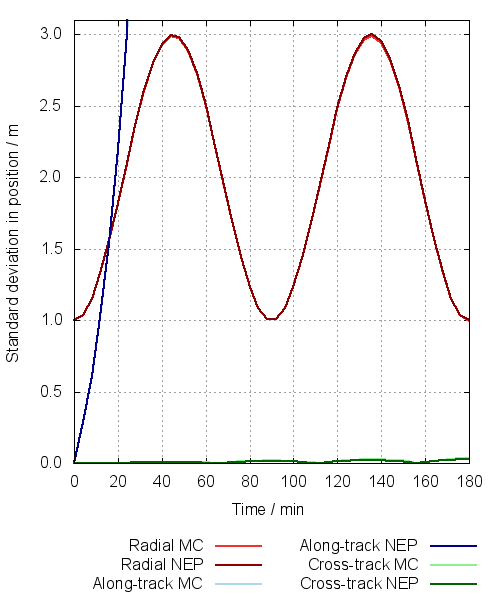
\includegraphics[width=0.4\textwidth]{2BJ2_1_rad.png}}
  \hspace{1cm}
  \subfigure[Velocity]{\label{fig:val-cov-scen2-01b} 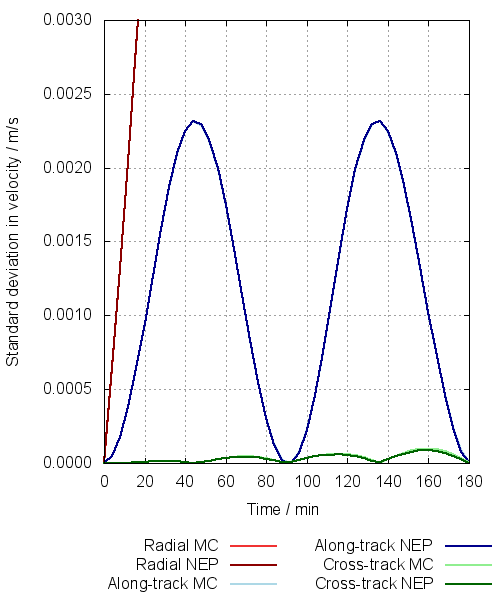
\includegraphics[width=0.4\textwidth]{2BJ2_1_vel.png}}
  \caption{Comparing MC analysis results to \neptune{} covariance matrix propagation using a \SI{60}{\second} integration step size for an initial radial error of \SI{1}{\metre} considering Earth's flattening. \label{fig:val-cov-scen2-01}}
\end{figure}
While the general behaviour in the radial and the along-track component are similar to the one already seen for the two-body case, including Earth's flattening introduces a drift in the orbit normal component. For the velocity normal component, the standard deviation is in the sub-mm/s region after two orbits, while for the position normal the standard deviation is in the centimeter regime. Note, that the simulation again was based on an initial error of \SI{1}{\metre} in the 
radial component.

In \fig{fig:val-cov-scen2-01} the results of \neptune{} closely align with the \gls{acr:mc} analysis. This gives evidence for the correct implementation of the partial derivatives as described in \sect{sec:propagation-covariance-set-integration-geopotential}. One could also look at what happens, if for the \gls{acr:mc} analysis once again the flattened Earth is used, while in \neptune{} the covariance matrix is integrated using the two-body scenario only. The result is shown in \fig{fig:val-cov-scen2-02}.
\begin{figure}[h!]
  \centering
  \subfigure[Position]{\label{fig:val-cov-scen2-02a} 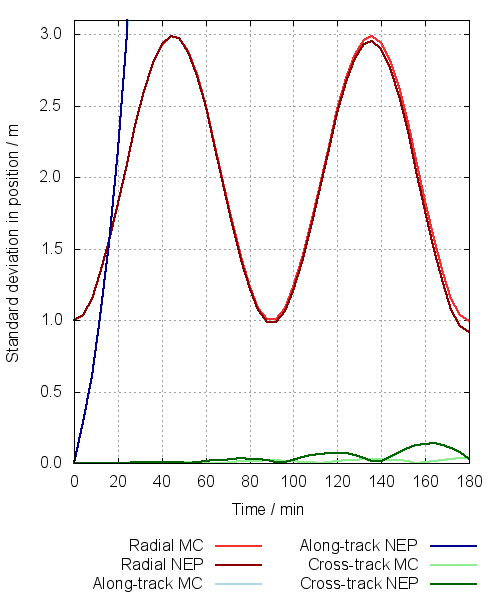
\includegraphics[width=0.4\textwidth]{2BJ2_2_rad.png}}
  \hspace{1cm}
  \subfigure[Velocity]{\label{fig:val-cov-scen2-02b} 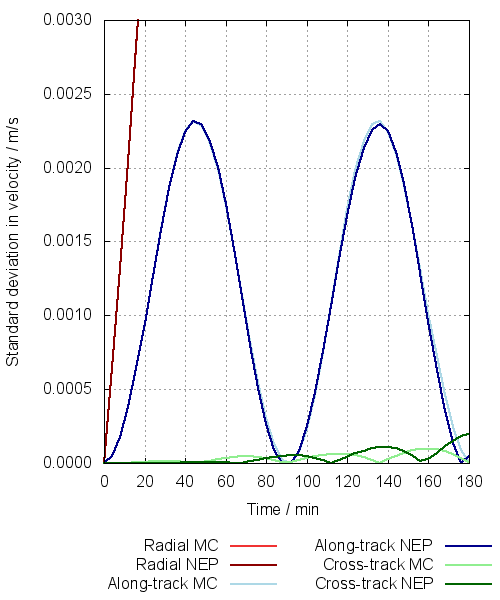
\includegraphics[width=0.4\textwidth]{2BJ2_2_vel.png}}
  \caption{Comparing MC analysis results (incl. Earth's flattening) to \neptune{} covariance matrix propagation using a \SI{60}{\second} integration step size for an initial radial error of \SI{1}{\metre} without Earth's flattening. \label{fig:val-cov-scen2-02}}
\end{figure}
It can be seen that there are significant differences in the radial and the cross-track component for the position error. The normal component even shows a phase shift of half an orbit. One question in this context is why the \neptune{} results for the two-body propagation look different than what was seen in 
\fig{fig:val-cov-scen1-01}. This is due to the fact that the state vector is propagated for a flattened Earth, while the covariance matrix is not. Thus, the state vector is different at each point in time when compared to the two-body propagation, which directly affects the integration of the covariance matrix, as it depends on the current radius vector for each integration step.

\paragraph{Scenario 3: Geopotential with order $\gls{sym:geo_n}>2$}

In \fig{fig:val-cov-scen3-01} the results are shown for a 36 $\times$ 36 geopotential for the same orbit and initial error of \SI{1}{\metre} in the radial position component as already in the previous examples.
\begin{figure}[h!]
  \centering
  \subfigure[Position]{\label{fig:val-cov-scen3-01a} 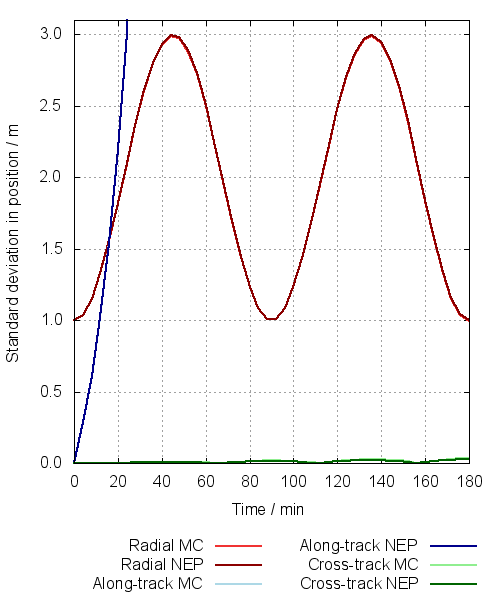
\includegraphics[width=0.4\textwidth]{2BGEOP_1_rad.png}}
  \hspace{1cm}
  \subfigure[Velocity]{\label{fig:val-cov-scen3-01b} 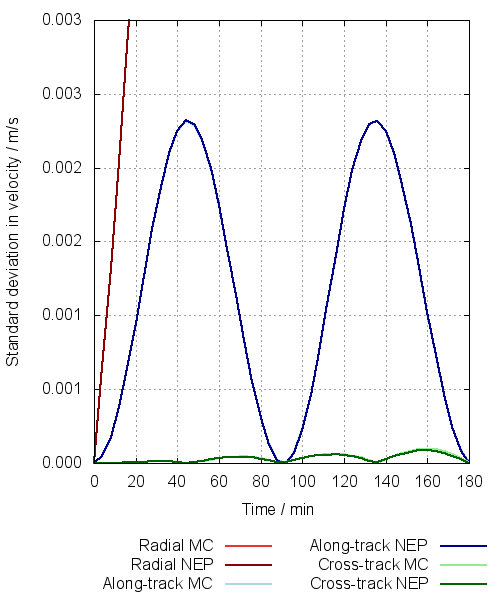
\includegraphics[width=0.4\textwidth]{2BGEOP_1_vel.png}}
  \caption{Comparing MC analysis results to \neptune{} covariance matrix propagation using a \SI{60}{\second} integration step size for an initial radial error of \SI{1}{\metre} considering a 36 $\times$ 36 geopotential. \label{fig:val-cov-scen3-01}}
\end{figure}
The situation looks very similar to the one for a second order geopotential as shown in \fig{fig:val-cov-scen2-01}. The differences are very small so that the 
same simulation was then performed for different orders of the geopotential and then to have a closer look on the normal component in 
\fig{fig:val-cov-scen3-02a} and the radial component in \fig{fig:val-cov-scen3-02b}.
\begin{figure}[h!]
  \centering
  \subfigure[Normal component]{\label{fig:val-cov-scen3-02a} 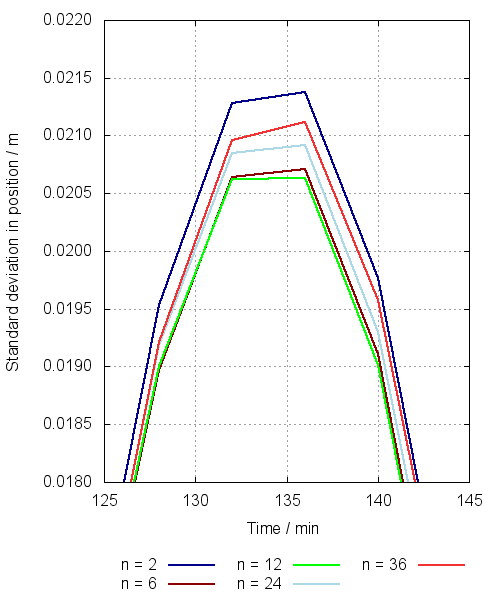
\includegraphics[width=0.4\textwidth]{2BGEOP_2_nor.png}}
  \hspace{1cm}
  \subfigure[Radial component]{\label{fig:val-cov-scen3-02b} 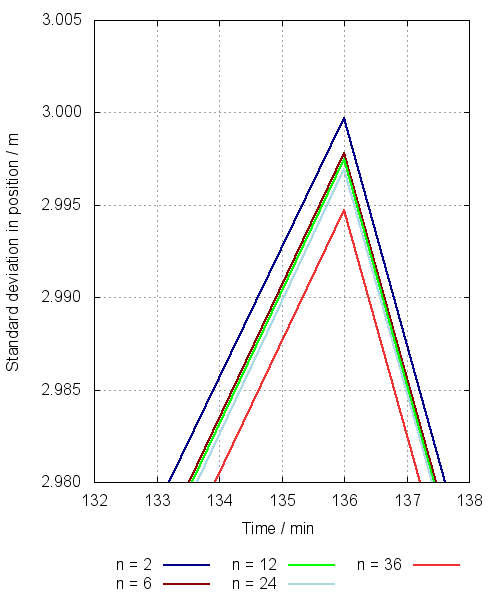
\includegraphics[width=0.4\textwidth]{2BGEOP_2_rad.png}}
  \caption{Sensitivity in covariance matrix propagation for varying order in the geopotential for an initial radial error of \SI{1}{\metre}. \label{fig:val-cov-scen3-02}}
\end{figure}
It can be seen that the error in the standard deviation for the normal component is in the order of magnitude of about \SI{1}{\milli\metre} when comparing a second order 
geopotential to higher orders. This corresponds to about \SI{5}{\percent} variation in this example as the second order geopotential accounts for \SI{2}{\centi\metre} after one and a half orbit. For the radial component the variation by using different order geopotentials is about \SI{5}{\milli\metre}. Note, however, that the number are only an example for that special orbit (\SI{300}{\kilo\metre}, \ang{50;;}) for a short time frame beyond the initial epoch.

In the same context, it is also interesting to look at orbits experiencing resonance effects due to the geopotential. An example shall be given for a \gls{acr:geo}.\todo[Covariance GEO example]{Provide example for GEO resonance effects in covariance matrix propagation.}

\paragraph{Scenario 4: Atmospheric drag}

For orbits experiencing significant drag perturbations it is possible to use additional terms in the variational equations to account for the resulting errors 
in the covariance matrix propagation. An example for a \SI{200}{\kilo\metre}, \ang{54;;} orbit with an initial error of about \SI{3}{\metre} in the along-track position component is shown in \fig{fig:val-cov-scen4-01}, with \neptune integrating only the two-body part for the covariance matrix.
\begin{figure}[h!]
  \centering
  \subfigure[Position]{\label{fig:val-cov-scen4-01a} 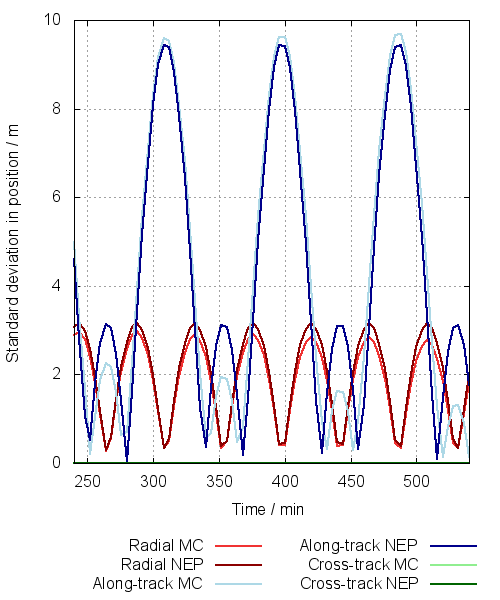
\includegraphics[width=0.4\textwidth]{DRAG_2_rad.png}}
  \hspace{1cm}
  \subfigure[Velocity]{\label{fig:val-cov-scen4-01b} 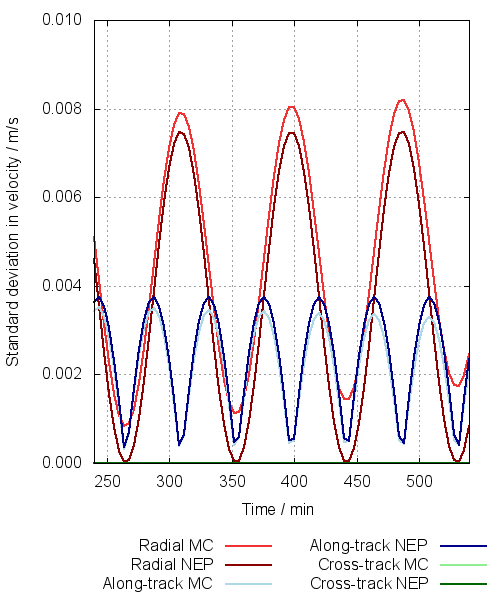
\includegraphics[width=0.4\textwidth]{DRAG_2_vel.png}}
  \caption{Drag perturbed orbit (\SI{200}{\kilo\metre}, \ang{54;;}) with \neptune not accounting for drag in the variational equations for an initial along-track position 
error of \SI{3}{\metre}. \label{fig:val-cov-scen4-01}}
\end{figure}
For the position error in \fig{fig:val-cov-scen4-01a} it can be seen that the error in the along-track component shows a drift of about \SI{10}{\centi\metre} per orbit. The 
increase is not accounted for by \neptune{}. Also, the radial component shows a significant difference after just a few orbits.

A similar behaviour can be observed for the velocity errors in \fig{fig:val-cov-scen4-01b}. The radial component shows a secular increase, while the 
along-track component decreases. Again both trends are not followed by \neptune{}, as expected.\todo[Explain drag deviations]{For the propagation of the covariance matrix, explain deviation with respect to the MC simulation}
 
%------------------------------------------------------------------------------
\addcontentsline{toc}{chapter}{References}

\nocite{iso8601}
\nocite{ccsds:ndm}

\bibliographystyle{plainnat}
\bibliography{../00-Templates/literature}

%------------------------------------------------------------------------------
\addcontentsline{toc}{chapter}{Glossary}

\chapter*{Glossary}
      
  \setglossarystyle{altlong4col}% 
  %\glossarystyle{aiaostyle}%
  \setlength{\glsdescwidth}{0.7\textwidth}
  %\setlength{\glspagelistwidth}{0.1\textwidth}
  \printnoidxglossary[type=symbolslist]			% latin
  %\printglossary[type=symbolslistgreek] 		% greek
  %\printglossary[type=symbolslistindex] 		% indices
  %\setglossarysection{chapter}						% 
  %\glstoctrue
  \printnoidxglossary[type=acronymlist]%mySymbolStyle]		% abbreviations
      
%------------------------------------------------------------------------------

\listoffigures
\addcontentsline{toc}{chapter}{\listfigurename}  

%------------------------------------------------------------------------------

\listoftables
\addcontentsline{toc}{chapter}{\listtablename}

%------------------------------------------------------------------------------

%\begin{appendix}
%  \include{annex-neptune}
%\end{appendix}

% \todos

\end{document}
